\documentclass[titlepage]{book}\usepackage{knitr}
\usepackage{bwstyle}

\title{\huge \textbf{ R- a tool for statistical analysis }\vspace{+1cm}  }
\subtitle{A modern introduction using tidyverse}
\author{{\LARGE \emph{Brian Williams}}\vspace{+1cm} \\
 Epidemiology and Global Health Unit,\\
 Department of Public Health and Medicine,\\
 Umeå University \vspace{+8cm}}
 

\date{\today}
\IfFileExists{upquote.sty}{\usepackage{upquote}}{}
\begin{document}



\maketitle

\frontmatter



%Template for children
% Change chunk name to chapter title
% ALl chunk names to be preceded by Tn or Ln  (where n is chapter or tutorial number)





\chapter*{Preliminaries}

\author{Brian Williams $<$\href{mailto:bjw649@gmail.com}%
{bjw649@gmail.com}$>$}

\section*{Installing R}
Download and install R from the  \href{http://www.r-project.org/}{R Homepage (http://www.r-project.org/)}.

Choose your computer, then operating system.  Use the 'base' install for Windows.

Use default values throughout the install.

While you are at the web site, you will see links to 'CRAN' -  go there and browse around and see what documentation is available.  You'll find lots of examples, tutorials etc.

\section*{Installing Rstudio}
\begin{enumerate}
\item{Go to the \href{http://www.rstudio.com/products/rstudio/download/}{Rstudio download page (http://www.rstudio.com/products/rstudio/download/)}.}
\item{When you get to the page, look for your computer/operating system under the heading 'Installers for ALL platforms'.  Click on yours.}
\item{You can choose a 'mirror' location for a download of the installer .exe file.}
\item{When the file is finished downloading. Click on it.}
\item{On a Windows platform you will be asked whether it's OK for the program to make changes to your computer. Click 'Yes'.}
\item{The installer opens up - close other applications, click 'Next'.}
\item{Accept the default settings - click 'Next' twice more then click 'Finish'.}
\end{enumerate}

An RStudio icon should now be available on your Desktop or Start menu (or equivalent - depending on your operating system). You can open RStudio by double-clicking on the icon.

The program will normally associate with files with extensions (.r, .R, .Rmd, .Rnw) where the case of the letters does not matter. Some software, (EndNote, for example), may also like to use one or more of those extensions, in which case you may like to choose the default?). You can change associations with file types by right clicking on a file with an extension of interest and selecting 'Properties'. The 'General' tab for Properties provides an opportunity to change the file association.

\section*{Getting the Course materials from GitHub}

The course material is in the R\_Course\_ folder. 


\begin{enumerate}
\item{\textbf{Resources} contains R\_Course\_Notes.pdf, miscellaneous resources, reference material etc. (Additional material may be added from time to time.)}\label{ResourcesFolder}
\item{\textbf{Data} contains the (moderate sized) datasets accessed by the code used in the course. (Some larger datasets will be accessed directly via the web.)}\label{DataFolder}
\item{\textbf{myR\_Code} will contain code you are developing during the course in tutorials etc.}\label{myCodeFolder}
\end{enumerate}

Now: 

\begin{enumerate}

\item {\textbf{Open RStudio}, by clicking on the icon.}

\item{From the File menu in RStudio, \textbf{open Lecture1.R} in the folder Resources/courseCode/. (Select [File -> Open File...].) In these notes, menu items will be indicated in square brackets with arrows as shown in the previous sentence.  The file \texttt{courseCode.R} contains all of the R code used in the notes.  Each Lecture and Tutorial is clearly identified. } 

\item{Open Lecture1.R. (Double click it). }

\item{Save this file in your myCode folder as Lecture1.R   [File-> Save As ....]}

\item{Use mouse/menu to \textbf{set the working directory}\index{RStudio!setting working directory} to the file location: [Session -> Set Working Directory -> To Source File Location]. You will see in the Console Pane (bottom left of the screen, see Figure~\ref{fig:Screenshot}) that the R function for this is \texttt{setwd()}\index{Core functions!setwd()}.   \textbf{This is an important step!}  Without it, R won't be able to find the data files, which have all been put in the Data folder which is found relative to the location of your Code folder.}

\end{enumerate}

The myCode folder is for your use.  I'll refer you to it from time to time. You can try code out in this folder and because of the file structure we have here, you'll be able to  access data in the Data folder in exactly the same way as we will do in class from the Code folder. If it get's too cluttered, create a Workspace folder in the R\_Course folder.
It will also be most convenient for you to put the new code for your assignments and the final exam in new folders called something like  'myAssignments' and 'myExamfolders' in the R\_Course folder, because then you'll be able to access the Data folder in the same way.

Now we're ready for the class!



%Template for children
% Change chunk name to chapter title
% ALl chunk names to be preceded by Tn or Ln  (where n is chapter or tutorial number)





\chapter{Preface}

\section{Original Preface by Brian Williams}

\author{Brian Williams $<$\href{mailto:bjw649@gmail.com}%
{bjw649@gmail.com}$>$}

This set of notes is intended as an introduction to the use of R for Public Health Students.  These notes are themselves an example of what can be achieved using one of the R User interfaces (RStudio) making use of the R package \texttt{knitr}. 

This is \textsl{not} a course on statistics - the expectation is that students will already have undertaken statistics courses (or be about to do so).  The emphasis here is on using a consistent subset of tools for preparing data for analysis and taking a preliminary look at it using tabulation of aggregates and visualization. The course will largely work with Hadley Wickham's 'tidyverse' packages. 

The course is limited to 13 Lectures of around one to two hours duration and 13 tutorials of similar length and as a consequence, there are limitations on the amount of material which can be covered.  I have tried to include appropriate references for further reading wherever discussion has been limited. 

Apart from the broader basics of R, I have included a view of the future of data science where it might be of interest to researchers in the Public Health. 

I have introduced the idea of Markdown in earlier courses, when RStudio converted it to nice HTML documents, but now newer versions of RStudio have made conversion to MS Word documents straightforward. 

To my way of thinking, the ease with which documentation of analytical processes can be maintained now, mandates that it should always be done.  Doing so aids the researcher in on-going recording of his or her own thinking, methodology, experimentation etc, and it is especially valuable when there are several approaches to choose from, requiring comparisons across perhaps complex procedures.  It is also an excellent way of providing fully accessible information for supervisors or collaborators.  Ultimately, this on-going, easy-to-do rigorous documentation provides a ready made basis for publication of completed research projects.

That said, with the rapidly changing experimental and analytical technology (changing data bases, analytical software etc), \emph{maintenance} of research in reproducible form is a significant issue.  My own view is that given the rapid development of research in general, and the potential maintenance work-load, that we should aim for 'reproducibility' to be maintained for around five years. In some very actively developing areas, three years may be more sensible, while in other more stable areas, a longer time-frame may be manageable without undue effort.  Maintaining reproducibility of software in cutting edge development will always require additional time and often may appear to be time spent for no productive outcome.

Bearing in mind that the intended audience of this course is not a group of computer scientists and some may have no experience in programming, I have taken a rather infomal approach trying to introduce examples early in the course which would motivate the audience, rather than beginning formally with an extensive set of definitions of language as one might find in a computer science text book. The \href{https://cran.r-project.org/doc/manuals/r-release/R-intro.pdf}{'An Introduction to R'} on the CRAN web page is an excellent more formal presentation if you prefer that approach.  I would like to think that these notes and that document complement one another. The draft 'R Language Definition' on the CRAN site is still more formal.

For those with no experience in R or programming, there may seem to be an overwhelming amount of information to comprehend. I can only advise you to not panic, relax, and don't worry about things you don't yet fully understand.  \emph{You cannot hope to be fully conversant in R in two weeks}! (I'm certainly not after dabbling for more than 10 years!) 

One of the most important lessons in the course will be to learn how to find answers to your R questions. Modern programmers work with multiple languages, editors, protocols, operating systems etc and cannot be expected to remember function arguments, specialised syntax etc. The real skill is being able to efficiently find out how to do something -  not remember how to do everything!

R too, has many thousands of functions.  Google usage is fundamental. There are a number of forums on the web which are generally very friendly and supportive if you are struggling with a problem. (Nabble, Stack Overflow are a good start.) You do need to follow forum protocols - almost all require a minimal example of your problem.

There are many other sources of examples of R code, most of which you will find using Google. Don't forget the CRAN \href{https://cran.r-project.org/}{pages} - there are a lot of resources there! 

The notes are a 'work-in-progress'.  They have largely been derived from my own work using R over the past ten years or so, and then cast into a teaching form in workshops and classes in the Epidemiology and Global Health Unit in the Department of Public Health and Medicine at Umeå University in the last couple of years.

I apologise for 'glitches' in the text (there will be many), but at the same time, I am hopeful that the notes (and classes) will provide a good basis for your venturing into R.

The notes will probably continue development in the next couple of years - look out for updates in the GitHub repo. \\


Brian Williams
 
 
March 2019.


\section{2nd Preface by Kaspar Meili}

Sadly, due to other commitments, Brian is no longer able to continue the development of the course files to the same extend as he used to. Luckily he agreed to let me help him maintaining the course and as a first step I uploaded the material to GitHub. We decided to publish the under the Creative Commons Attribution 4.0 International License CC BY 4.0. \href{https://creativecommons.org/licenses/by/4.0/}. 

\cleardoublepage
\phantomsection
\addcontentsline{toc}{chapter}{Table of contents}
\tableofcontents
\cleardoublepage
\mainmatter


\begin{knitrout}
\definecolor{shadecolor}{rgb}{0.969, 0.969, 0.969}\color{fgcolor}\begin{kframe}
\begin{alltt}
\hlkwd{library}\hlstd{(knitr)}
\hlkwd{set_parent}\hlstd{(}\hlstr{"../tidyRcourseBook.rnw"}\hlstd{)}
\hlkwd{library}\hlstd{(tidyverse)}
\hlstd{warn} \hlkwb{<-} \hlnum{FALSE}
\hlstd{EVAL} \hlkwb{<-} \hlnum{TRUE}
\end{alltt}
\end{kframe}
\end{knitrout}



\chapter{Lecture 1 - Introduction to R and RStudio }\label{L1}
\section*{- and a glimpse of what's coming!}

\author{Brian Williams $<$\href{mailto:bjw649@gmail.com}%
{bjw649@gmail.com}$>$}

\section{Summary}
In this session there will be a brief introduction to RStudio and reading, manipulating, cross-tabulating and visualizing data from dataframes using the \emph{tidyverse} package in RStudio.

\textbf{Note:} In this lecture some advanced features of R will be demonstrated. \textbf{Don't worry about what appears to be complex commands}. You will be shown how to easily step through the code and see what comes from it! 

RStudio is the most widely used integrated development environment (IDE) for R and provides excellent support for documenting code for reproducibility.

\subsection{Tidyverse}
Tidyverse is a suite of modern R software, largely developed by Hadley Wickham and colleagues at RStudio, which aims to reduce R's learning curve by providing a more consistent way of dealing with dataframes. 

Not all the software in tidyverse is limited to dataframes, but that is its broad goal.   Tidyverse is still under development, though what we will use is well tried and tested. 

There are still many procedures of interest to us in 'Core' R, which currently lie outside tidyverse and we will use these as the need arises. 

Check out the freely available \href{https://r4ds.had.co.nz/index.html}{web version of the book} "R for data science" by Hadley and Garret Grolemund \cite{Wickham2016}. This course is inspired by the approach in that book.  Much of the material in this course is extracted and simplified from an earlier course aimed at research students in the Medical Faculty. The earlier course notes are available in the resources folder (R4researchFeb2016.pdf) and may provide expanded background on many topics. The R4researchFeb2016.pdf notes are also live-indexed and have a live table of contents, so you should be able to find things in those notes reasonably easily.

\section{Preliminaries}

Load and install R, RStudio and extract the folders from R\_Course.zip (available on the Course pages on Cambro) in a convenient folder on your computer. (Extracting will normally create a new folder called R\_Course).

\section{Getting started}

\textbf{Note that you will follow the steps in this section at the beginning of every Lecture and Tutorial.}

Assuming you have taken all the steps in the Preliminaries section:

Navigate to your R\_Course folder. It should contain 3 folders, Data, myCode, Resources and files called ReadMe.pdf, Preliminaries.pdf and RCourseOutlineRev2019.pdf. 

\textbf{Open} R\_Notes.pdf, located in your Resources folder.

You will need to open the Resources folder and then the R\_Notes.pdf at the beginning of each class. You will be able to follow the class presentation and use the live links in the notes for each Lecture and Tutorial. Note that the index is also live-linked so you should be able to find your way about without too much trouble. (If you are using Acrobat and Windows, [Alt <-] pressed together will take you back from the index to where you clicked on the index link.)

Now: 

\begin{enumerate}

\item {\textbf{Open RStudio}, by clicking on the icon.}

\item{From the File menu in RStudio, \textbf{open the folder courseCode} in the folder R\_Course/Resources  (Select [File -> Open File...].) In these notes, menu items will be indicated in square brackets with arrows as shown in the previous sentence.  The folder \texttt{courseCode} contains all of the R code used in the notes.  Each Lecture and Tutorial is clearly identified.} 

\item{Double click on Lecture1.R and it will open in The Edit Pane  of your RStudio window (see Figure~\ref{fig:Screenshot}).}

\item{Use [File -> Save As...] in the file menu to save the file in your myRcode folder.}  

\item{Use mouse/menu to \textbf{set the working directory}\index{RStudio!setting working directory} to the file location: [Session -> Set Working Directory -> To Source File Location]. You will see in the Console Pane (bottom left of the screen, see Figure~\ref{fig:Screenshot}) that the R function for this is \texttt{setwd()}\index{Core functions!setwd()}.}

\end{enumerate}

\begin{figure}[!ht]
\graphicspath{{./Images/}}
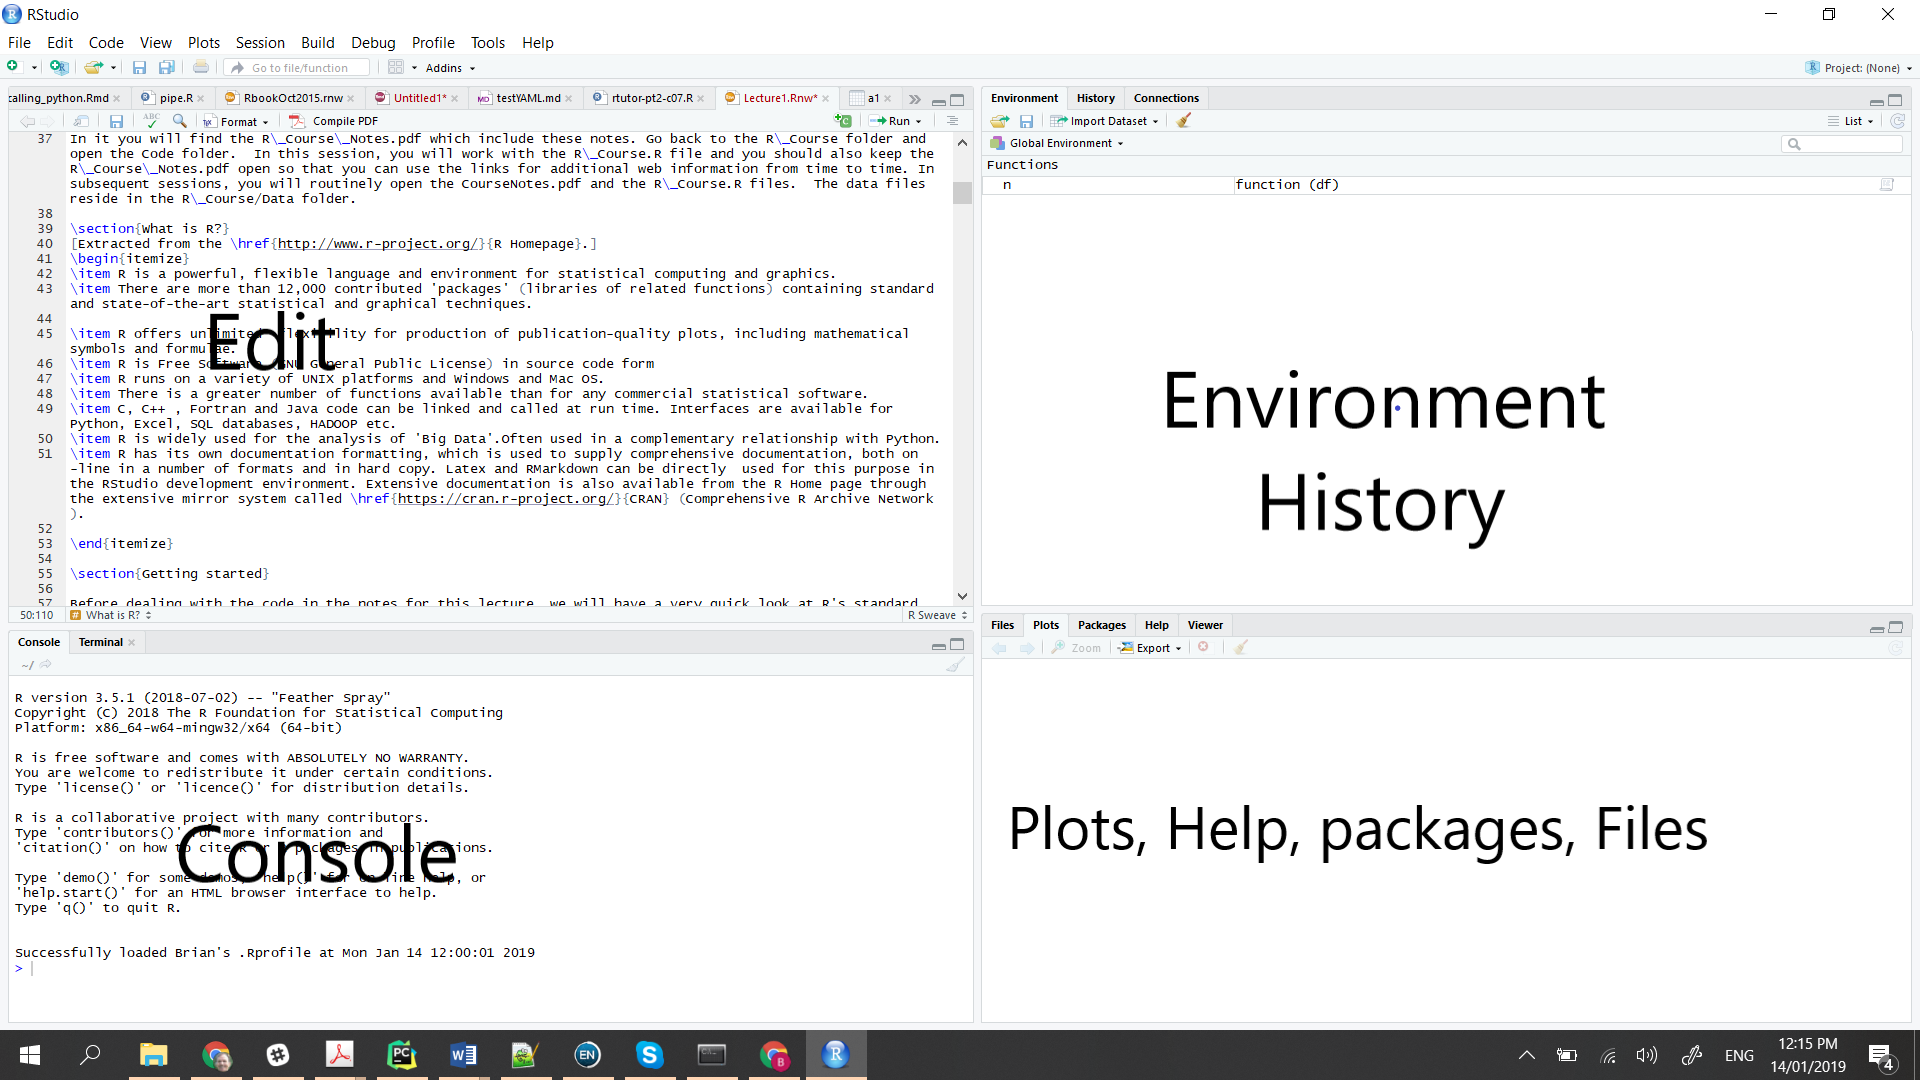
\includegraphics[width = 16cm, height = 8cm]{Screenshot1.png}
\caption{The four panes in the RStudio window}
\label{fig:Screenshot}
\end{figure}

This sets your working directory to the myCode folder. \textbf{This is an important step!}  Without it, R won't be able to find the data files, which have all been put in the Data folder which is found relative to the location of your myCode folder. Both the Data folder and your myCode folder are in the R\_Course folder (their 'parent' folder). If you are not clear take a look at Section~\ref{DataStructure} in the Appendix.

You will see that the top left window pane of the RStudio interface now contains the Lecture1.R file.   We refer  to this pane as the \textbf{Edit pane}\index{RStudio!Edit pane} or 'script' pane or window (See Figure~\ref{fig:Screenshot}.  Notice that the name of the file is shown on a 'tab' above the window. You can use this pane to edit a number of different scripts using the tabs, and from this pane you can run selected code directly, by clicking on the 'Run' button on the pane's toolbar.

If you compare the text in beige, below in these notes, with the first 'block' in the Edit pane, you will see that in the notes, each line is preceded by '\#\#'. This is just a decoration generated by the software for these notes. The proper R statements without '\#\#' are in your Lecture1.R file, as displayed in the edit pane of RStudio.

Beneath the Edit pane, is the \textbf{Console pane}\index{RStudio!Console Pane}(See Figure~\ref{fig:Screenshot}), in which the evaluated R commands will appear. It has a '>' symbol as a prompt, which indicates that the Console Pane is ready for your next command.  You can also paste commands into this pane for execution, or edit a previous command using the up-arrow to retrieve it. 

If you see a '+' prompt, it is an indication that you have entered an incomplete command and R is waiting for the rest of the command. If you can see what you have left out, enter it and press return and the command will be executed.  Sometimes it will not be clear what is missing and you may have to start again -  in that situation to return to the '>' prompt you must press the 'Escape' key.  

To clear everything in the console window, press 'Ctrl+L'.

The top right pane (see Figure~\ref{fig:Screenshot}) is the \textbf{Environment/History pane}\index{RStudio!Environment/History pane} (selectable using the tabs). The environment will contain basic information about variables which the user has introduced. There are two groups. At the top is 'Data' which consists of two-dimensional arrays (dataframes look like a spreadsheet table) and underneath are 'Variables' which are all other data objects defined by the user in the session.

The history tab contains the sequence of R commands which the user has entered during the session (and earlier). You can execute these directly by selecting them with a mouse click and then clicking on the tool above, labelled 'To Console'. If you want to insert these commands in your edit window, click where you wanted the commands inserted and then click on the 'To Source ' button in the History Pane.


The bottom right pane has a variety of displays (Files, Plots, Packages and Help) indicated and accessed by the tabs.

Now before we begin -

The text in the sections of the notes in the coloured (beige?) boxes between the dashed lines:

\# - - - - - - - - - - - - - - - - - - - - - - - - - - - - - - - - - - - - - - - - -

are sequences of R commands (scripts). You will find an extraction of all these scripts in Lecture1.R, Tutorial2.R etc in the Resources/Course\_R\_Code folder.
Scripts may include comments. Lines preceded with the \# symbol (like the dashed line above) may be used to explain to a reader what the script is doing - or (as here) provide a way of separating or identifying lines of text. These lines preceded with the \# symbol are ignored by R's interpretation (computation) of the script.

You can run the example scripts in Lecture1.R in three ways.
(The easiest way is the last one!)

First: \textbf{select} (highlight) the code using your mouse.

Then \textbf{copy} (using the Windows shortcut, \texttt{Ctrl-c)}. (\texttt{Command-c on a Mac})

Now \textbf{click} in the Console window of RStudio (the window below), and \textbf{paste} the code (\texttt{Ctrl-v}). (Mac: \texttt{Command-v})

If nothing happens, in the console, press the return/enter key.

\textbf{Second:}, after highlighting the code, \textbf{click} on the 'Run' button\index{RStudio!Run button} near the top right of the Edit window.

\textbf{Third (best):} Place the cursor on the first line and press \texttt{Ctrl-enter}. The code in that line will execute and the cursor will move down to the next line of code. Repeat pressing \texttt{Ctrl-enter} until you have stepped through as much of the code as you want to execute.

Try these three methods with the following 4 lines of script:

\begin{knitrout}
\definecolor{shadecolor}{rgb}{0.969, 0.969, 0.969}\color{fgcolor}\begin{kframe}
\begin{alltt}
  \hlcom{##Normally distributed N(0,1) variates, mean, var}
  \hlcom{#-----------------------------------------------------------------------------------}
\hlkwd{set.seed}\hlstd{(}\hlnum{1121}\hlstd{)}  \hlcom{# set a seed for pseudo-random number generation}
\hlstd{(x} \hlkwb{<-} \hlkwd{rnorm}\hlstd{(}\hlnum{20}\hlstd{))}   \hlcom{# creates a vector, x, containing 20 N(0,1) variates}
\hlkwd{mean}\hlstd{(x)}         \hlcom{# computes the mean of the sample}
\hlkwd{var}\hlstd{(x)}          \hlcom{# computes the variance of the sample}
\hlcom{#----------------------------------------------------------------------------------}
\end{alltt}
\end{kframe}
\end{knitrout}

  Now \textbf{CLICK in the edit window} away from the selection to deselect (remove the highlight)!!!!

  If you don't, the highlighted code will be \textbf{LOST} as it is replaced by your next typed characters in the edit window.

It's easy to make this mistake (I do it frequently!) but if you realise you have done it, the edit menu provides an 'undo' item which will get the lost characters back for you. (\texttt{Ctrl Z} also works - and you can undo\index{RStudio!undo} several actions by pressing \texttt{Ctrl z} repeatedly). As with all kinds of editing on computers, it's a good idea to save your edited file using (\texttt{Ctrl S}) frequently. You can save \textbf{all} the files you have opened in RStudio, using (\texttt{Ctrl Alt S}).

\section{HELP!!}
There are various ways of getting help in R.
\begin{itemize}
\item{\texttt{??graph} searches the documentation for the word 'graph' and lists findings in the Help window (bottom right).}
\item{\texttt{?plot} is used to find help for a \emph{function} (the function \texttt{plot}, in this case). }
\item{Similarly, \texttt{help(fn)}\index{Core functions!help()} finds the documentation associated with the function named \texttt{fn}. It acts exactly the same as the previous one (the question mark form).}

\item{\texttt{example(fn)}\index{Core functions!example()}  prints a number of examples of the use of the function in the Console window.}
\item{Some packages have an introductory document called a 'vignette' which can be accessed with the function \texttt{vignette()}\index{Core functions!vignette()}, but you should start with \texttt{browseVignettes()}!}
\item{Try: \texttt{vignette('lmtest-intro')}.}
\item{\texttt{data()}\index{Core functions!data()} lists available data sets (and is used to load datasets, too).}
\end{itemize}

For more complex problems go to the Help window (click on the Help tab if it is not currently selected) and click on the Home icon (the picture of a little house in the tool bar of this window) and you will see links  to some of the various documentation on the CRAN web site.
Otherwise on the CRAN website itself you can look at \href{http://cran.r-project.org/doc/contrib/Torfs+Brauer-Short-R-Intro.pdf}{reference material} on the CRAN site.

.......or simply \emph{use Google} (often the best way for more complicated queries) If your problem is a little complicated, Google is likely to find something on the 'stackoverflow' site.  Take your time looking at material on this site.  Because there is a significant level of control on posting, the responses are more reliable than many other sites on the web. Look for a big green 'tick' for the best solution to a questioner's problem.

\section{Functions}
We have already used some \textbf{functions}\index{Functions!using} in R.  Functions are fundamental to the use of commands. Commands always use functions, though it may not always be apparent.

\begin{itemize}
\item{Functions appear as a character string followed by parenthesis (curved brackets) containing zero or more items called \textbf{arguments} separated by commas. These argument control the way the function behaves.}

\item{Most functions have multiple  arguments, which have been given \textbf{default values}. If you don't specify an argument when you 'call' (i.e. use) the function, its default value will be used.}

\item{We can change the defaults by specifying values for the arguments when we call the function. Arguments in all functions can be changed in this way but must conform to the requirements of the function, which may require, for example, that an argument be of a particular type, or that its length match that of another argument.}

\end{itemize}

To see how a function (say) \texttt{mean()}\index{Core functions!mean()} is used, enter \texttt{help(mean)} in the Console window and look at the output in the Help pane to the right. Help for functions can also be accessed by typing e.g. \texttt{?mean} in the Console window. Try it with \texttt{?sd}

There are other examples of functions in the \href{https://cran.r-project.org/doc/manuals/r-release/R-intro.html#Simple-examples}{on-line Manual} "An introduction to R" on the CRAN website. 

\section{Data frames: reading data and investigating them}\index{Core functions!data()}

In this section we'll see the power of R, but we won't try to look in detail at the function useage - that'll come later, so don't worry too much about the syntax of the commands (functions).

There are a number of functions which allow reading of data sets from other statistical software like SAS and Stata (see the package 'foreign'), but for the moment we'll deal with reading our data from a .csv file, perhaps created by spreadsheet software.\index{Data frame!reading from .csv} We are going to focus our efforts on a single R package called tidyverse, which you will see is implemented by calling the \texttt{library} function with tidyverse as its argument.  Before doing so, however, we need to install the package.

\subsection{Installing packages} 

Tidyverse contains a suite of modern R packages, mostly authored by Hadley Wickham and his colleagues at RStudio. Tidyverse focuses on the preparation, analysis and vizualization of dataframes - and that is the focus of this course.  

\subsubsection{Installing tidyverse}
Installing a package is easy. Go to [Tools->Install packages ...]. Type the name of the package (tidyverse) (it should be predicted) and then click on install. You will see some activity in the console window and then a message indicating that the installation is successful, followed by the Console Pane's standard prompt '>'.

When that's all done, go to the packages pane and click on the 'Packages' tab at the top. Use the window slider at the side or the search at the top to find the tidyverse package in the list. Click in the box on the left and you will see that the library command has been used in the Console window of RStudio. [The libary command will also include the directory path of all your installed packages.] Click on the blue name tidyverse and you will be taken to the help page for the package. All packages will have some kind of help file like this. The Description file may be a bit too terse, but if you click on the User guides..... link, you will usually find more digestible infomation.

\subsection{Reading a dataframe using the tidyverse package \texttt{readr}}

In \texttt{tidyverse}, the standard function for reading a .csv file is \texttt(read\_csv).

\begin{knitrout}
\definecolor{shadecolor}{rgb}{0.969, 0.969, 0.969}\color{fgcolor}\begin{kframe}
\begin{alltt}
  \hlcom{##Reading and summarising data frames}
  \hlcom{#----------------------------------------------------------------------------------}
\hlkwd{library}\hlstd{(tidyverse)}
\hlstd{bP}        \hlkwb{<-} \hlkwd{read_csv}\hlstd{(}\hlkwc{file}\hlstd{=}\hlstr{"../Data/BackPain.csv"}\hlstd{,} \hlkwc{na} \hlstd{=} \hlkwd{c}\hlstd{(}\hlstr{""}\hlstd{,}\hlstr{" "}\hlstd{,}\hlstr{"NA"}\hlstd{))}      \hlcom{# (1), (2), (3), (4)}
\end{alltt}


{\ttfamily\noindent\itshape\color{messagecolor}{\#\# Parsed with column specification:\\\#\# cols(\\\#\#\ \  .default = col\_character(),\\\#\#\ \  age = col\_double(),\\\#\#\ \  bmi = col\_double(),\\\#\#\ \  waistc = col\_double(),\\\#\#\ \  comorb = col\_double(),\\\#\#\ \  disability = col\_double(),\\\#\#\ \  height = col\_double()\\\#\# )}}

{\ttfamily\noindent\itshape\color{messagecolor}{\#\# See spec(...) for full column specifications.}}\begin{alltt}
\hlkwd{glimpse}\hlstd{(bP)}
\hlstd{bP}             \hlcom{# bP is a tibble so only 10 lines are printed (and a limited number of variables, too)}
\end{alltt}
\end{kframe}
\end{knitrout}
  \subsubsection{Notes:}
\begin{enumerate}
\item{The <- symbol assigns the output from the function on the right to the variable named on the left.}
\item{\texttt{read\_csv()}\index{Tidyverse functions!read\_csv()} reads a '.csv' formatted file specified in the first argument.}
\item{The na = argument tells the function to process missing, blank or NA as NA.}
\item{Note that the use of ../ in the specified file path finds the data file by going firstly to the folder of the parent of the working directory. The parent folder is the R\_course folder. There it finds the Data folder in which it finds the file "BackPain.csv"!)}
\item{\texttt{read\_csv()} assumes the data has a \textsl{header row} which is used to create column (Variable) names.}
\item{The output from \texttt{read\_csv()} is a form of data frame object called a 'tibble' (More about this later.)}
\item{Have a look at the help window for \texttt{read\_csv()}. (Type ?read\_csv in the Console window.) You can use  additional 'arguments' to specify na's, column header (variable) names etc.}
\item{Note if comma is used to specify decimal points in your file you can use {\texttt{read\_csv2()}}, which assumes a semi-colon separator, or {\texttt{read\_tsv()}} for tab separated files. If something else has been used, see the docuentation on {\texttt{read\_delim()}}.}
\item{You can have a look at the data file in the Edit Pane by going to the Environment Pane (top right-hand-side) and clicking on bP - (it's at the top in a section headed 'Data'. Clicking on the little blue arrow will expand a summary in the Environment pane.)}
\item{You can also import data from SAS, SPSS, or Stata  with your mouse! [File-> Import Dataset]. Check the package \texttt{haven} for details of the handling of different formats.}
\item{ Specifying the name of a standard dataframe lists the entire df - not a good idea if it's large! Tibbles restrict the print.}
\end{enumerate}

The first thing we notice from our \texttt{glimpse()} in the Console below, is that \texttt{bP} has 34122 observations (rows) and 24 variables (columns). The columns are a mixture of 'dbl' and 'chr'.  We'll talk about this more as time goes on, but for the moment we're going to convert all the 'chr' variables to what R calls \textsl{factors} - these are called categorical variables in some other statistical environments.

We'll also demonstrate the power of dplyr when using \textsl{pipes} in the next code chunk - in a single assignment we convert all the character variables to factors, remove all the NA's in the dataframe, and create a new variable for the waist/height ratio of the subjects. It looks very complex - but really its just like learning another language (Yes, I know - Swedish is very difficult!)
\label{filter}\label{mutate}\index{tidyverse filter}\index{tidyverse mutate}

\begin{knitrout}
\definecolor{shadecolor}{rgb}{0.969, 0.969, 0.969}\color{fgcolor}\begin{kframe}
\begin{alltt}
\hlstd{bP} \hlkwb{<-} \hlstd{bP} \hlopt                                      \hlcom{# (1)}
  \hlkwd{mutate_if}\hlstd{(is.character, as.factor)} \hlopt          \hlcom{# (2) }
  \hlkwd{filter}\hlstd{(}\hlkwd{complete.cases}\hlstd{(.))} \hlopt                   \hlcom{# (3)}
  \hlkwd{mutate}\hlstd{(}\hlkwc{waistHtRatio} \hlstd{= waistc}\hlopt{/}\hlstd{height)}            \hlcom{# adds a new variable called waistHtRatio  (4)}
\end{alltt}
\end{kframe}
\end{knitrout}

\subsubsection{Notes:}
\begin{enumerate}
\item{The \%>\%  'pipes' the dataframe on its left to the first argument of the function on its right (in this case on the next line).}
\item{The \texttt{mutate\_if} function is converting those variables which are characters, to factors}
\item{The \texttt{complete.cases} function can selectively remove records with NA's in specified variables - in this case it is removing all rows with 1 or more NA's}
\item{\texttt{mutate} creates a new variable as a function of existing variables.}
\end{enumerate}

In general when using the complete.cases function, one should select removal only for those rows where at least one of the variables of interest is NA. Here we effectively chose ALL the variables.  If you look in the environment pane, you will see that our 30,000 or so records have been reduced to 12,200! We continue for demonstration purposes! [We'll look at this more carefully later!]

\subsection{Tabulation}

Here we introduce a new package based on \texttt{tidyverse} called \texttt{janitor}.  This package simplifies some of the basic tabulation processes that we might be familiar with from other statistical software.

\subsubsection{One-way table}

\begin{knitrout}
\definecolor{shadecolor}{rgb}{0.969, 0.969, 0.969}\color{fgcolor}\begin{kframe}
\begin{alltt}
\hlkwd{library}\hlstd{(janitor)}
\end{alltt}


{\ttfamily\noindent\itshape\color{messagecolor}{\#\# \\\#\# Attaching package: 'janitor'}}

{\ttfamily\noindent\itshape\color{messagecolor}{\#\# The following objects are masked from 'package:stats':\\\#\# \\\#\#\ \ \ \  chisq.test, fisher.test}}\begin{alltt}
\hlstd{c1} \hlkwb{<-} \hlstd{bP} \hlopt
      \hlkwd{tabyl}\hlstd{(country)}
\hlstd{c1}
\end{alltt}
\end{kframe}
\end{knitrout}

\subsection{Two-way table}
\begin{knitrout}
\definecolor{shadecolor}{rgb}{0.969, 0.969, 0.969}\color{fgcolor}\begin{kframe}
\begin{alltt}
\hlstd{c2} \hlkwb{<-} \hlstd{bP} \hlopt
      \hlkwd{tabyl}\hlstd{(country, eduS)}
\hlstd{c2}
\end{alltt}
\end{kframe}
\end{knitrout}

...and some people are more familiar with percentages:

\begin{knitrout}
\definecolor{shadecolor}{rgb}{0.969, 0.969, 0.969}\color{fgcolor}\begin{kframe}
\begin{alltt}
\hlstd{c3} \hlkwb{<-} \hlstd{bP} \hlopt
    \hlkwd{tabyl}\hlstd{(country, agegr)} \hlopt
    \hlkwd{adorn_percentages}\hlstd{(}\hlstr{"row"}\hlstd{)} \hlopt
    \hlkwd{adorn_pct_formatting}\hlstd{(}\hlkwc{digits} \hlstd{=} \hlnum{2}\hlstd{)}
\hlstd{c3}
\end{alltt}
\end{kframe}
\end{knitrout}
The levels of factors by default are listed alphabetically, sometimes there is a sensible order so we change it:

\begin{knitrout}
\definecolor{shadecolor}{rgb}{0.969, 0.969, 0.969}\color{fgcolor}\begin{kframe}
\begin{alltt}
 \hlstd{bP} \hlkwb{<-} \hlstd{bP} \hlopt
       \hlkwd{mutate}\hlstd{(}\hlkwc{eduS} \hlstd{=} \hlkwd{fct_relevel}\hlstd{(eduS,}\hlstr{"No primary"}\hlstd{,}\hlstr{"Compl Primary"}\hlstd{,}
                                 \hlstr{"Compl Sec/HS"}\hlstd{,} \hlstr{"Compl Uni/Coll"}\hlstd{),}
                     \hlkwd{fct_relevel}\hlstd{(bmi4,} \hlstr{"Underweight"}\hlstd{,}\hlstr{"Normal"}\hlstd{,}
                                 \hlstr{"Pre-Obese"}\hlstd{,} \hlstr{"Obese"}\hlstd{))}
\hlcom{#-------------------------------------------------------------------------------}
\end{alltt}
\end{kframe}
\end{knitrout}

We'll visualize the bmi4 below.
\begin{knitrout}
\definecolor{shadecolor}{rgb}{0.969, 0.969, 0.969}\color{fgcolor}\begin{kframe}
\begin{alltt}
\hlstd{c3} \hlkwb{<-} \hlstd{bP} \hlopt
    \hlkwd{tabyl}\hlstd{(country, eduS)} \hlopt
    \hlkwd{adorn_percentages}\hlstd{(}\hlstr{"row"}\hlstd{)} \hlopt
    \hlkwd{adorn_pct_formatting}\hlstd{(}\hlkwc{digits} \hlstd{=} \hlnum{2}\hlstd{)}
\hlstd{c3}
\end{alltt}
\end{kframe}
\end{knitrout}

\begin{knitrout}
\definecolor{shadecolor}{rgb}{0.969, 0.969, 0.969}\color{fgcolor}\begin{kframe}
\begin{alltt}
\hlstd{bySex} \hlkwb{<-} \hlkwd{group_by}\hlstd{(bP,country,residence, sex)} \hlopt
       \hlkwd{summarise}\hlstd{(} \hlkwc{meanDisability} \hlstd{=} \hlkwd{mean}\hlstd{(disability),} \hlkwc{sdDisability}\hlstd{=}\hlkwd{sd}\hlstd{(disability))}
\hlcom{# kable(bySex)}
\end{alltt}
\end{kframe}
\end{knitrout}

\section{Visualization}

Visualization in the tidyverse uses a package developed by Hadley Wickham called \texttt{ggplot2}. This package is widely regarded in the computing industry as one of the very best.  However, it preceded the tidyverse ideas of dataframes in and out of functions and so does not quite conform to the idealised model. It produces static two-dimensional plots, which in modern web-computing is 'old-hat' but Wickham has modern developments underway. 
\texttt{ggplot2} is based on a 'Grammar of Graphics' (hence the gg.). This allows the user to add layers of information on a single plot.  It takes a little bit of learning, but there is plenty of help on the web and the results are wonderful.
Here are a few examples using the backPain data. (We'll take a closer look at this code later.)


\begin{knitrout}
\definecolor{shadecolor}{rgb}{0.969, 0.969, 0.969}\color{fgcolor}\begin{kframe}
\begin{alltt}
\hlstd{pp1} \hlkwb{<-} \hlkwd{ggplot}\hlstd{(bP,} \hlkwd{aes}\hlstd{(}\hlkwc{x}\hlstd{=bmi,} \hlkwc{fill}\hlstd{=agegr))} \hlopt{+}
  \hlkwd{geom_histogram}\hlstd{(}\hlkwc{binwidth} \hlstd{=} \hlnum{2.5}\hlstd{)} \hlopt{+}
  \hlkwd{facet_grid}\hlstd{(country} \hlopt{~} \hlstd{sex,}\hlkwc{scales}\hlstd{=}\hlstr{"free_y"}\hlstd{)}
\hlstd{pp1}
\end{alltt}
\end{kframe}
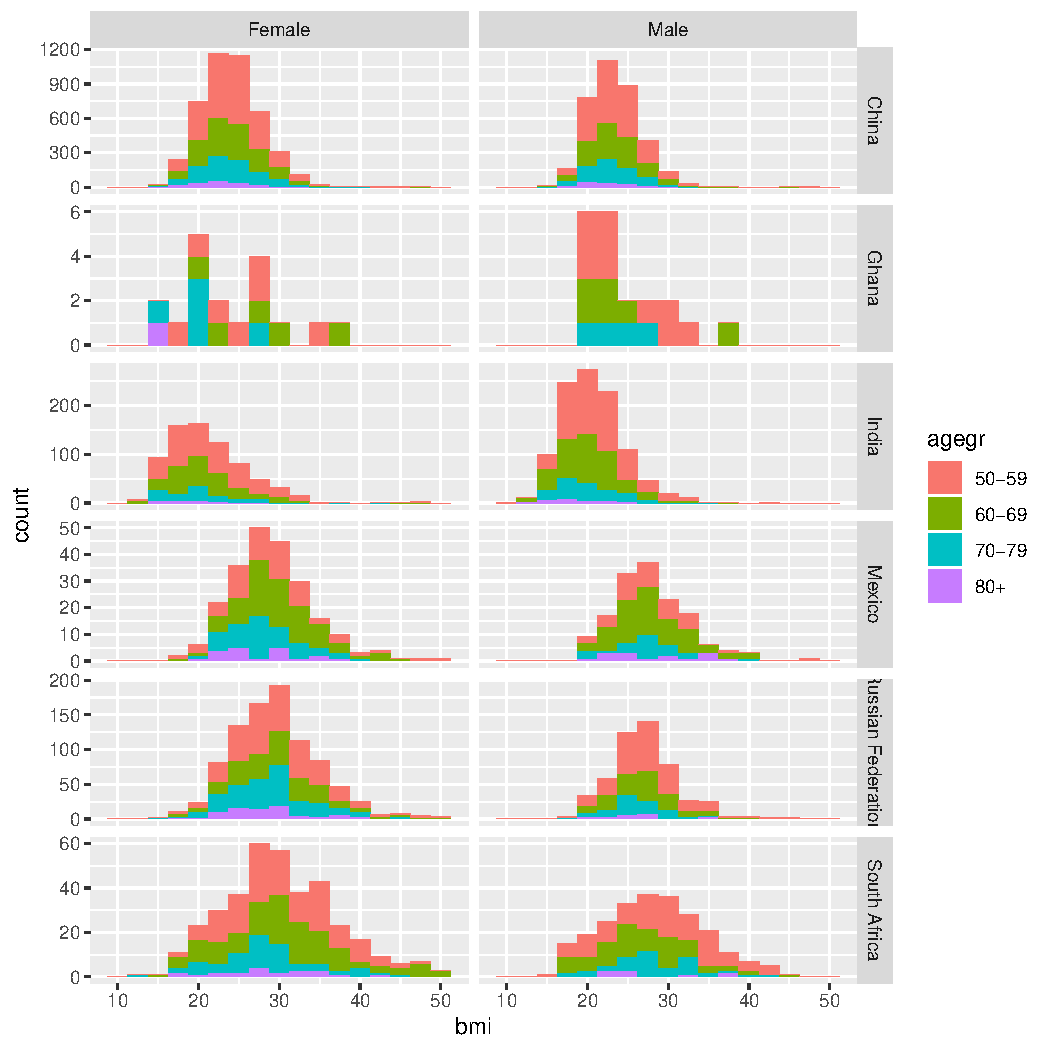
\includegraphics[width=\maxwidth]{figure/L1_FacetedHistograms-1} 

\end{knitrout}

Note the 'free' y-axis. Its not obvious at first glance that China has much more data than South Africa.  An annotation on the plot of the total numbers would draw immediate attention to this. Note too that Ghana's data set (after removal of the NA's) is \textsl{very} small. For some unexplained reason, the Ghana data has very few height measurements even though these are necessary for comutation of BMI.
Let's have a look at the data for disability vs age.

\begin{knitrout}
\definecolor{shadecolor}{rgb}{0.969, 0.969, 0.969}\color{fgcolor}\begin{kframe}
\begin{alltt}
 \hlstd{bP} \hlkwb{<-} \hlstd{bP} \hlopt \hlkwd{mutate}\hlstd{(}\hlkwc{bmi4} \hlstd{=} \hlkwd{factor}\hlstd{(bmi4,} \hlkwc{levels} \hlstd{=}
                                     \hlkwd{c}\hlstd{(}\hlstr{"Underweight"}\hlstd{,}\hlstr{"Normal"}\hlstd{,} \hlstr{"Pre-Obese"}\hlstd{,} \hlstr{"Obese"}\hlstd{)))}
\hlstd{p} \hlkwb{<-} \hlkwd{ggplot}\hlstd{(bP,} \hlkwd{aes}\hlstd{(}\hlkwc{x} \hlstd{= age,}  \hlkwc{y} \hlstd{= disability ,}\hlkwc{color} \hlstd{= residence,} \hlkwc{shape} \hlstd{= sex))} \hlopt{+}
  \hlkwd{geom_point}\hlstd{()} \hlopt{+}
  \hlkwd{facet_grid}\hlstd{(country}\hlopt{~}\hlstd{bmi4)}
\hlstd{p}
\end{alltt}
\end{kframe}
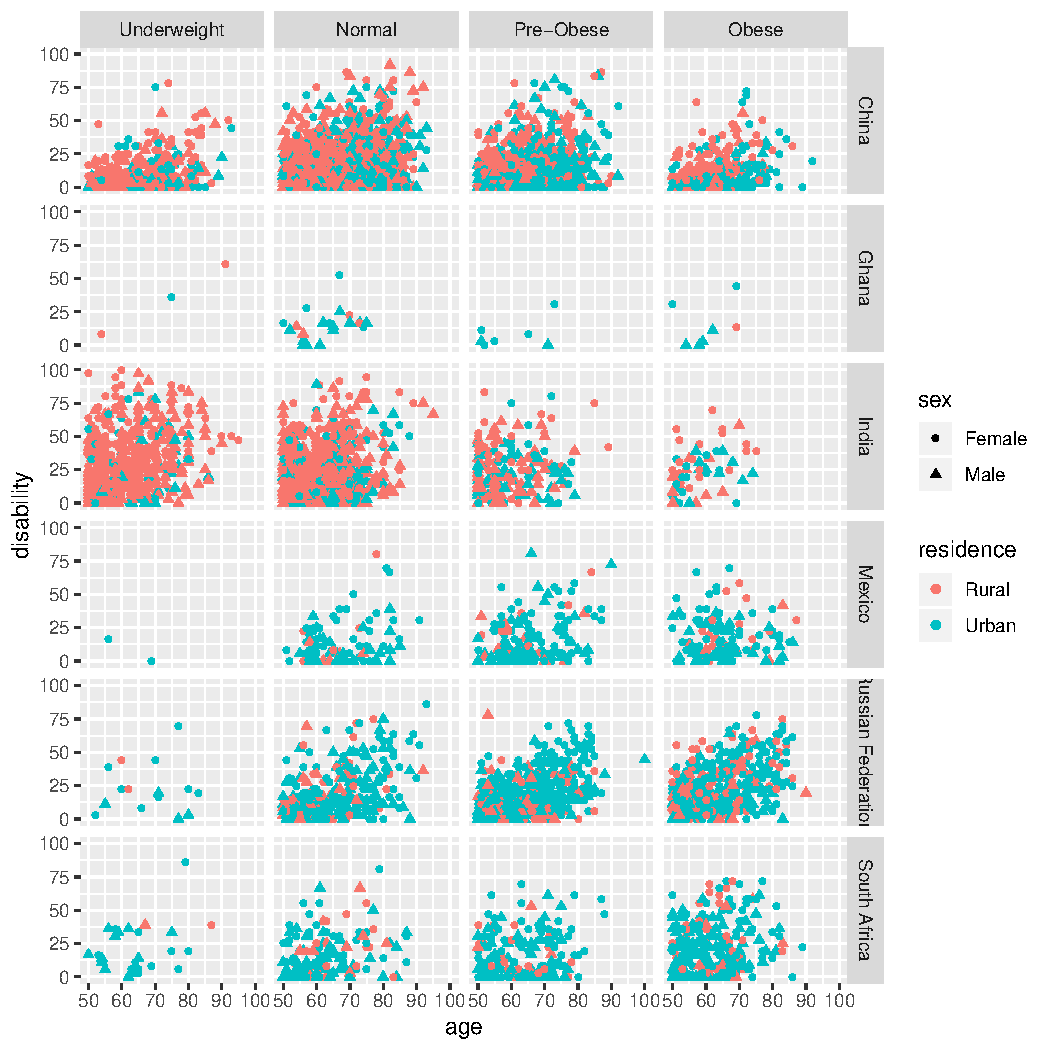
\includegraphics[width=\maxwidth]{figure/L1ScatterFacet-1} 

\end{knitrout}



%\printindex






\chapter{Tutorial 1 - Rstudio, dataframes, packages and file handing}

\author{Brian Williams $<$\href{mailto:bjw649@gmail.com}%
{bjw649@gmail.com}$>$}

\section{Preliminaries}

Go to the Resources folder and open the courseCode.R file.  Find "Tutorial1". Copy it.  Open RStudio. Open a New R script.Paste Tutorial1 into the edit pane of the New file and save it in your myRcode folder as 'Tutorial1.r'.

\section{Working Directory}\index{Working directory}

In RStudio you can change to your working directory of choice using the menu as follows: [Session->Set working directory\...] or you can use the standard R command, \texttt{setwd()}\index{Core functions!setwd()}.  If you use the menu to set the working directory to the directory of the current file, using [Session->Set working directory->To Source File Location], you will see the  \texttt{setwd()} function used in the Console Pane.


\begin{knitrout}
\definecolor{shadecolor}{rgb}{0.969, 0.969, 0.969}\color{fgcolor}\begin{kframe}
\begin{alltt}
\hlkwd{getwd}\hlstd{()}
\end{alltt}
\end{kframe}
\end{knitrout}
Amongst other things, \texttt{getwd()} can be helpful in reporting results if you have a complex file system and potential confusion some months later when looking at the output.
If you want to see the files in the working directory, then use the function \texttt{dir()}\index{Core functions!dir()}.

\begin{knitrout}
\definecolor{shadecolor}{rgb}{0.969, 0.969, 0.969}\color{fgcolor}\begin{kframe}
\begin{alltt}
\hlkwd{dir}\hlstd{()}
\end{alltt}
\end{kframe}
\end{knitrout}

Note that even though it has no arguments you must include the parentheses when using this function.

\section{Importing external files}\index{Importing external files}


\begin{knitrout}
\definecolor{shadecolor}{rgb}{0.969, 0.969, 0.969}\color{fgcolor}\begin{kframe}
\begin{alltt}
\hlkwd{library}\hlstd{(tidyverse)}
\hlstd{bP}        \hlkwb{<-} \hlkwd{read_csv}\hlstd{(}\hlkwc{file}\hlstd{=}\hlstr{"../Data/BackPain.csv"}\hlstd{,} \hlkwc{na} \hlstd{=} \hlstr{""}\hlstd{,} \hlkwc{comment} \hlstd{=} \hlstr{'#'}\hlstd{,} \hlkwc{skip} \hlstd{=} \hlnum{0}\hlstd{)}
            \hlcom{# bP is a tibble so only 10 lines are printed (and a limited number of variables, too)}
\hlkwd{select}\hlstd{(bP,alcohol)}
\hlstd{bP} \hlkwb{<-} \hlstd{bP} \hlopt \hlkwd{mutate_if}\hlstd{(is.character, as.factor)}
\hlkwd{select}\hlstd{(bP,alcohol)}
\end{alltt}
\end{kframe}
\end{knitrout}


\begin{enumerate}
\item The argument list begins with a 'relative' file name. The '..' means go to the parent folder of the working directory then look for a folder  called 'Data' and select the file called 'BackPain.csv' in that directory.

\item In R, missing data is indicated with the string 'NA' (without the quotation marks). \texttt{na.strings = ""}: This is a 'nothing entered' value for the \texttt{na.strings} parameter.  This argument provides values of NA for the data frame entries which have the characters listed for this parameter, i.e. with our setting, those entries which have a 'blank' (white space), are made 'NA'. In some other datasets, a missing value might be indicated by a symbol such as '*' or '\#' and this argument let's you specify that.


\item You can use the \texttt{col\_names} argument in two ways. If you set \texttt{col\_names = FALSE}, \texttt{read\_csv} skips the first line of the data file and constructs column names with the form X1, X2, X3 etc. The other way of using \texttt{col\_names} is to set it to a vector of your own choice of column names, i.e. something like: {col\_names = c("x", "k", "w", ...)}

\end{enumerate}


\section{Cleaning up NA's - rough approach!}

Now we will do a very rough cleanup of the data, by simply removing all records which have one or more missing data items (NA's). We'll begin by summing the total number of NA's, then removing the rows in which they are present, and then repeating the sum check to ensure that we have indeed removed all the NA's.

\begin{knitrout}
\definecolor{shadecolor}{rgb}{0.969, 0.969, 0.969}\color{fgcolor}\begin{kframe}
\begin{alltt}
\hlkwd{sum}\hlstd{(}\hlkwd{is.na}\hlstd{(bP))}   \hlcom{# compute number of NA's}
\hlstd{bP} \hlkwb{<-} \hlstd{bP} \hlopt \hlkwd{drop_na}\hlstd{()}  \hlcom{# Use this to remove all cases (rows) containing at least one NA from}
\hlcom{#  The non-tidyverse way  bP <- na.omit(bP)}
\hlkwd{sum}\hlstd{(}\hlkwd{is.na}\hlstd{(bP))}     \hlcom{#check whether all NA's are removed}
\hlcom{#----------------------------------------------------------------------------------}
\end{alltt}
\end{kframe}
\end{knitrout}

  \subsubsection{Notes:}

\begin{itemize} 

\item{\texttt{is.na(X)}\index{Core functions!is.na()} returns a vector of \texttt{TRUE} or \texttt{FALSE} for every element of X. When summed, TRUE = 1, FALSE =0.}

\item{\texttt{omit.na()}\index{Core functions!omit.na()} and \texttt{tidyR::drop\_na()} are very powerful and produces a 'complete cases' data frame - but be careful, you may lose a lot of data!  Look at the new size of bP!}

\item{Where logicals are included in a numerical computation, R assumes \texttt{TRUE} = 1, \texttt{FALSE} = 0, so \texttt{sum(is.na(bP))} computes the total number of NA's in the data frame.}
\end{itemize}


\subsection{Referencing data frame elements}\index{Data frame!referencing elements}

Outside of tidyverse, the preferred way of referring to variables is with the '\$' notation, e.g.  \textbf{dfn\$varName} -  where dfn is the data frame name, and varName is the variable name. You can also refer to it using the number of the column in square brackets. If you use the name of the column, you will still correctly access it if you change the column numbering in some other operation.  However, there are times when using column numbers is convenient.

We use square brackets with row, column indexes to select individual elements of the data frame.
\textbf{bP[3,2]} is the 3rd element of the variable in the second column.

If the comma is kept but either index is omitted, all elements of the missing index are selected. Thus \textbf{bP[,2]} refers to all values recorded for the variable in the second column and \textbf{bP[2,]} refers to all items recorded in the second row.

In operations where a number of variables are to be accessed, it is sometimes easier to use their column number with the \texttt{bP[colNumber]} notation.

Suppose that in the back pain dataset, we carelessly assume the 11th column is named "bmi".

\begin{knitrout}
\definecolor{shadecolor}{rgb}{0.969, 0.969, 0.969}\color{fgcolor}\begin{kframe}
\begin{alltt}
\hlcom{##Column selection in data frames  *******Use names!!!!!!}
\hlcom{#-----------------------------------------------------------------------------------}
\hlkwd{head}\hlstd{(bP[}\hlnum{11}\hlstd{])}      \hlcom{#print out the 1st 6 elements of bmi....OOOPS!}
\hlkwd{head}\hlstd{(bP}\hlopt{$}\hlstd{bmi)}       \hlcom{#print out the 1st 6 elements of bmi}
\hlkwd{names}\hlstd{(bP)}          \hlcom{# Ah - bmi is col 12!}
\hlcom{#-----------------------------------------------------------------------------------}
\hlstd{bP} \hlopt \hlkwd{select}\hlstd{(bmi)}
\end{alltt}
\end{kframe}
\end{knitrout}


\subsection{Imports from other statistical packages}
The R package 'foreign' enables reading of data stored by Minitab, S, SAS, SPSS, Stata, Systat and others. You can also export (Write) files from R in the formats of some other packages, including Stata.  Objects such as data frames can be saved as ASCII (text) files to produce .csv files which can be read from almost any other program.  ASCII files, however, will be much larger than binary files like .rda (see below under Save).  Here's an example of reading from a Stata file.  We'll save the file as a .Rdata file and use it in Tutorials later. This file contains some additional variables.

\begin{knitrout}
\definecolor{shadecolor}{rgb}{0.969, 0.969, 0.969}\color{fgcolor}\begin{kframe}
\begin{alltt}
\hlkwd{library}\hlstd{(haven)}
\hlstd{bPx} \hlkwb{<-} \hlkwd{read_dta}\hlstd{(}\hlstr{"../Data/BackPainData_1.dta"}\hlstd{)}
\hlkwd{summary}\hlstd{(bPx)}
\hlkwd{save}\hlstd{(bPx,} \hlkwc{file} \hlstd{=}  \hlstr{"../Data/BackPainData_1.Rdata"}\hlstd{)}
\end{alltt}
\end{kframe}
\end{knitrout}


\section{Listing and removing  objects}\index{Objects!listing}\index{Objects!removing}

Let's create a 'vector' object so we can see how objects are listed and removed in R and RStudio. 


\begin{knitrout}
\definecolor{shadecolor}{rgb}{0.969, 0.969, 0.969}\color{fgcolor}\begin{kframe}
\begin{alltt}
\hlstd{vect1} \hlkwb{<-} \hlstd{bP}\hlopt{$}\hlstd{agegr}                                \hlcom{#1 Created a vector object  }
\hlkwd{ls}\hlstd{()}                                      \hlcom{#2 List all objects in WD}
\hlkwd{objects}\hlstd{()}                                                 \hlcom{#2 List all objects in WD}
\hlkwd{remove}\hlstd{(vect1)}                                            \hlcom{#3 Remove object 'vect1'}
\hlkwd{ls}\hlstd{()}
\end{alltt}
\end{kframe}
\end{knitrout}


\begin{enumerate}
\item The \$ notation has been used to select the column of the variable \texttt{agegr}. The code has assigned the vector of the variable to 'vect1'.

\item Objects are listed by using either \texttt{ls()}\index{Core functions!ls()} or \texttt{objects()}.\index{Core functions!objects()} You must include the parentheses when using these functions. Note too, that the objects are already listed in the Environment Pane in RStudio.

\item Objects can be removed using \texttt{remove()}\index{Core functions!remove()} or its abbreviated form, \texttt{rm()}.\index{Core functions!rm()}
\item{ \textbf{All variables} in the Environment can be removed by clicking on the little 'brush' icon in the Environment toolbar.}

\end{enumerate}

\section{Saving objects and workspaces to files, reloading}

The \texttt{save()} function is straightforward.

With respect to the data we have been looking at here, we could do the following:
\begin{knitrout}
\definecolor{shadecolor}{rgb}{0.969, 0.969, 0.969}\color{fgcolor}\begin{kframe}
\begin{alltt}
\hlkwd{save}\hlstd{(}\hlstr{"bP"}\hlstd{,} \hlkwc{file}\hlstd{=}\hlstr{"BackPain.RData"}\hlstd{)}
\hlkwd{dir}\hlstd{()}
\end{alltt}
\end{kframe}
\end{knitrout}


Now let's remove the object bP from our environment, and restore it by loading the saved file "BackPain.RData".\index{Core functions!save()}

\begin{knitrout}
\definecolor{shadecolor}{rgb}{0.969, 0.969, 0.969}\color{fgcolor}\begin{kframe}
\begin{alltt}
\hlkwd{remove}\hlstd{(bP)}
\hlkwd{ls}\hlstd{()}
\end{alltt}
\end{kframe}
\end{knitrout}
Notice that bP is gone from the Environment pane as well as missing from the output of \texttt{ls()}.

\begin{knitrout}
\definecolor{shadecolor}{rgb}{0.969, 0.969, 0.969}\color{fgcolor}\begin{kframe}
\begin{alltt}
\hlkwd{load}\hlstd{(}\hlstr{"BackPain.RData"}\hlstd{)}
\hlkwd{ls}\hlstd{()}
\end{alltt}
\end{kframe}
\end{knitrout}
Now we have it back.

Notice that the loaded data takes the \emph{original object name}, not the file name. If you want to rename\index{Objects!renaming} the new object, you must firstly copy it and then remove the old object:

\begin{knitrout}
\definecolor{shadecolor}{rgb}{0.969, 0.969, 0.969}\color{fgcolor}\begin{kframe}
\begin{alltt}
\hlstd{bP2} \hlkwb{<-} \hlstd{bP}
\hlkwd{ls}\hlstd{()}
\hlkwd{rm}\hlstd{(bP)}
\hlkwd{ls}\hlstd{()}
\end{alltt}
\end{kframe}
\end{knitrout}
R is clever about this.  Even though you will see both objects listed, R does not actually make a copy (which if your object is very large might cause a memory problem). When the R interpreter reaches the \texttt{rm()} function it \emph{then} simply changes the name of the object in memory.

The \texttt{save()} function allows saving of multiple objects either named at the beginning of the command itself, or the first argument can be a list of the objects to be saved in the form of a character vector of the object names.
 At the conclusion of a session \texttt{save.image(".Rdata")} is automatically offered.  This saves the entire workspace so that when R is next opened, the workspace can be loaded with \texttt{load(".Rdata")}\index{Core functions!load()}. Pay attention to the directory in which this is taking place! RStudio auto-loads the .Rdata file in your Documents folder at start-up. If you load the wrong .Rdata file, you can remove all files easily by clicking on the 'clear' tool in the Environment pane.
Sometimes, you will want to save a workspace or a large cleaned data frame under another name so that it is not inadvertently opened or deleted (\texttt{save(myDataFrame,file =  "myFileName")})\index{Core functions!save()}. You can actually save a list of objects in this way (\texttt{save(myDataFrame, a, b, c, file = "myFileName")}).  You can also choose to save the data in ASCII (text) format (\texttt{save(myDataFrame,file = "myFileName", ASCII=TRUE)})\index{Core functions!save()}. Any time you want to load these back into your working environment, simply \texttt{load( "myFileName")}.  Try it out!
There are a few functions that are important to know for saving workspace data to disk and subsequently re-loading it. You can see what data objects and functions you have created in the Environment pane. You can list them in the console pane using \texttt{objects()}.  You can remove a number of objects with the \texttt{rm()}\index{Core functions!rm()} command.


There are two other related functions which can be very useful in the construction of self-contained \emph{minimal reproducible examples}.  These functions are \texttt{dput()}\index{Core functions!dput()} and \texttt{dget()}.\index{Core functions!dget()}

\begin{knitrout}
\definecolor{shadecolor}{rgb}{0.969, 0.969, 0.969}\color{fgcolor}\begin{kframe}
\begin{alltt}
\hlstd{t1} \hlkwb{<-} \hlstr{"The cow jumped over the moon, the little dog laughed to see such fun"}
\hlkwd{dput}\hlstd{(t1,} \hlkwc{file}\hlstd{=t1)}
\hlstd{t2} \hlkwb{<-} \hlkwd{dget}\hlstd{(t1)}
\hlstd{t2}
\end{alltt}
\end{kframe}
\end{knitrout}

See \texttt{help(dput)} for more information.


\section{Packages and their data}\index{Packages}
Packages can be readily installed in RStudio, using the Tools menu: [Tools-> Install Packages...] then enter the package name in the middle edit window - leave the others. You will see some activity in the Console pane as the package downloads.\index{RStudio!installing packages}. Try installing the package \texttt{dplyr} - we will use it frequently in this course.

To get an overview of the functions associated with a package, for example dplyr\index{Package!dplyr}, use the help function with a package argument: \texttt{help(package = "dplyrL")}\index{Core functions!help()}.

On a Windows PC, installation of a package loads it into a folder in your computer's Documents folder. It will be called something like 'Documents/R/Win-library/3.1' (for Version 3.1). It can be useful to know the location of this folder if you are updating R.

Packages may contain quite large datasets, so R assumes that you will not automatically want to load all your installed datasets into memory.  To \emph{load} a particular installed package, say ggplot2\index{Package!ggplot2}, you use the command \texttt{library(ggplot2)}\index{Core functions!library()}. (Within functions, we use \texttt{require(ggplot2)}\index{Core functions!require()}, which returns FALSE if the package cannot be found and allows the programmer to exit gracefully!) This makes the package's functions and datasets available. RStudio lists all the installed packages in the bottom-right pane under the Packages tab.  You can access a package by ticking (clicking in) the box alongside the package name in that pane as an alternative to the \texttt{library(ggplot2)} command. You will see that a number of base packages are already ticked.

\subsection{The base data sets}

If you use the command \texttt{search()}\index{Core functions!search()}, you will see that these packages are on R's search path, which it uses when looking for data files. To find out what's available, type \texttt{data()}\index{Core functions!data()}. You can access data sets in these packages with the command e.g. \texttt{data(Nile)}. When this command is executed, the dataset is 'soft-loaded'.  Until you actually do something with Nile, it is still not loaded into memory. Until you use it, in RStudio in the top right pane with the Environment tab active, it will appear annotated in grey with <Promise>. After typing, for example, \texttt{summary(Nile)}, into the console window, the data are loaded and the dimensions of Nile appear in the Environment pane.

\begin{knitrout}
\definecolor{shadecolor}{rgb}{0.969, 0.969, 0.969}\color{fgcolor}\begin{kframe}
\begin{alltt}
\hlcom{## Using the data in the base release of R}
\hlkwd{search}\hlstd{()}
\hlkwd{library}\hlstd{(}\hlkwc{help}\hlstd{=datasets)}
\hlkwd{data}\hlstd{(Nile)}
\hlkwd{summary}\hlstd{(Nile)}
\hlkwd{plot}\hlstd{(Nile)}
\end{alltt}
\end{kframe}
\end{knitrout}

Notice that the \texttt{library()} function can be used to obtain help about a package as shown in this chunk.

Finally, it is worth noting that sometimes there are identical function names in different packages which have been loaded and to distinguish them, we  specify the package appropriate to the function, using the operator '::'.  So to if we think there is any risk of ambiguity we can refer to function \texttt{fn1()} from package \texttt{packageName} as \texttt{packageName::fn1()}.\index{Operators!::}.

%\printindex





\chapter{Lecture 2 - Vectors, dataframes}\index{Core!Factors}

\author{Brian Williams $<$\href{mailto:bjw649@gmail.com}%
{bjw649@gmail.com}$>$}

\section{Summary}

In this lecture there will be a brief discussion of some of the important terminology and components of R - objects (vectors, data frames), functions, notation conventions etc.
We will then look at a self documenting language called RMarkdown, which allows incorporation of R code directly  into documentationwhich can be transformed into HTML for web pages or MS Word or PDF form.

\section{Logistics}

Go to the Code folder and open the courseRcode folder.  Find "Lecture2.R". Save As.. in the myRcode folder.

As before, use mouse/menu to set the working directory to the file location: [Session->Set Working Directory->To Source File Location]. \textbf{This is an important step in every class!}


\section{Vectors}\index{Vectors}\label{vectors}

Vectors play an important role in our data analysis because the data in each of our variables \textsl{is} a vector.  A vector is a list of data which are all of the same type - numbers, character strings or factors.  We can use vectors to construct dataframes or we can extract vectors from dataframes.
Because they have such an important role, we'll take a brief look at how they are dealt with in R.


\subsection{Elementary construction of vectors}
The function \texttt{c(some comma-separated list of object arguments)}\index{Core functions!c()} \texttt{combines} the arguments into a single new object (if possible!). It is one of \textbf{the most widely used of all R functions} and is used very often when you want to use a group of numbers or characters as an argument in some other function. This is one you MUST remember. Its murky origins in Unix, mean that it is also sometimes referred to as \emph{concatenate}.

If you use \texttt{c()} to combine  a list of arguments which have different classes, R tries to figure out how the user might want to combine the arguments with a common type. (Remember our standard \emph{atomic vector} must have all elements of the same class.)

Here are some examples:
\begin{knitrout}
\definecolor{shadecolor}{rgb}{0.969, 0.969, 0.969}\color{fgcolor}\begin{kframe}
\begin{alltt}
\hlcom{##Automatic variable conversion (Coercion)}
\hlcom{#----------------------------------------------------------------------------------}
\hlstd{A} \hlkwb{<-} \hlnum{11}
\hlstd{B} \hlkwb{<-} \hlnum{7}
\hlstd{C1} \hlkwb{<-} \hlstd{A} \hlopt{+} \hlstd{B}
\hlstd{a} \hlkwb{<-} \hlkwd{c}\hlstd{(A,B,C1)}  \hlcom{# Concatenates or binds the arguments into a vector}
\hlstd{a}
\hlkwd{str}\hlstd{(a)}     \hlcom{#  Very useful standard command in R for printing the structure of an object}
\hlstd{d} \hlkwb{<-} \hlstr{"Victoria"}
\hlstd{t} \hlkwb{<-} \hlkwd{c}\hlstd{(d,}\hlstr{'geoff'}\hlstd{,} \hlstr{'Lars'}\hlstd{)}
\hlstd{t}
\hlstd{t} \hlkwb{<-} \hlkwd{c}\hlstd{(t,}\hlstr{'Stig'}\hlstd{)}
\hlstd{t}
\hlstd{t} \hlkwb{<-} \hlkwd{c}\hlstd{(t,A)}
\hlstd{t}
\hlstd{t} \hlkwb{<-} \hlkwd{c}\hlstd{(}\hlnum{1}\hlstd{,}\hlnum{2}\hlstd{,}\hlstr{"Eugenie"}\hlstd{)}
\hlkwd{str}\hlstd{(t)}
\hlcom{#----------------------------------------------------------------------------------}
\end{alltt}
\end{kframe}
\end{knitrout}
Note that R is OK with converting the integer g to a numeric to form the four element vector, a.

Elements of vectors are accessed as well a displayed, using square brackets as we shall see below.

The operator ':' is very useful for creating vectors of simple sequences and selecting sequential elements in vectors.


It is often useful to know how long vectors are; the function \texttt{length(v)}\index{Core functions!length()} returns the length of v.

\begin{knitrout}
\definecolor{shadecolor}{rgb}{0.969, 0.969, 0.969}\color{fgcolor}\begin{kframe}
\begin{alltt}
\hlcom{##vector manipulations}
\hlcom{#----------------------------------------------------------------------------------}
\hlkwd{length}\hlstd{(a)}
\hlstd{ss} \hlkwb{<-} \hlnum{5}\hlopt{:}\hlnum{22}      \hlcom{# creates a vector, ss, whose elements are the sequence 5,6... to 22}
\hlstd{ss}
\hlstd{ss[}\hlnum{6}\hlstd{]}
\hlkwd{length}\hlstd{(ss)}
\hlcom{# and a little bit tricky:}
\hlstd{sss} \hlkwb{<-} \hlstd{ss[ss} \hlopt{>} \hlnum{20}\hlstd{]}   \hlcom{# assigns those values of ss which are greater than 8 to a}
\hlcom{# new vector sss}
\hlstd{sss}
\hlkwd{sum}\hlstd{(sss)}
\hlcom{#-----------------------------------------------------------------------------------}
\end{alltt}
\end{kframe}
\end{knitrout}
We refer to commands like  \texttt{sss <- ss[ss > 20]} as 'filtering').  We will see in \ref{L3} that there is a tidyverse function called 'filter' which is used for dataframes.
The function \texttt{sum()}\index{Core functions!sum()} returns the summation of the elements of the specified vector.

We'll spend more time later looking at filtering and data preparation but let's jump ahead and load up a real data-set.  'Data frame' is R jargon  equivalent to a 'data set' in most other statistical software.


R has a range of objects which can store data of various kinds.  The simplest is the \textbf{vector} which is simply an ordered collection of data items of a single type. If you want an important example, think of it as the observations of a variable in your data set. We will do a lot of manipulation of data and much of it involves operating with vectors.

\subsection{Addressing vector elements}\index{Vectors!addressing elements}\label{vecAddress}

The number of items in the vector is its length. The individual item in the sixth position in a vector, \texttt{aa} can be accessed by reference to \texttt{aa[6]}.

We can access a sub-vector consisting of the 3\textsuperscript{rd}, 4\textsuperscript{th} and 5\textsuperscript{th} components using \texttt{aa[3:5]}, or \texttt{aa[c(3, 4, 5]}. The latter can be used to access any set of indices.

Using a minus '-' sign in front of an index is used to delete that element.

\begin{knitrout}
\definecolor{shadecolor}{rgb}{0.969, 0.969, 0.969}\color{fgcolor}\begin{kframe}
\begin{alltt}
\hlstd{cc} \hlkwb{<-} \hlkwd{c}\hlstd{(}\hlnum{1}\hlstd{,} \hlnum{4}\hlstd{,} \hlnum{98}\hlstd{,} \hlnum{17}\hlstd{,} \hlnum{43}\hlstd{,} \hlnum{172}\hlstd{,} \hlnum{34}\hlstd{,} \hlnum{67}\hlstd{,} \hlnum{58}\hlstd{,} \hlnum{143}\hlstd{,} \hlnum{27}\hlstd{,} \hlnum{72}\hlstd{,} \hlnum{44}\hlstd{,} \hlnum{88}\hlstd{,} \hlnum{83}\hlstd{)}
\hlstd{cc}
\hlstd{cc[}\hlkwd{c}\hlstd{(}\hlnum{3}\hlstd{,}\hlnum{5}\hlstd{,}\hlnum{8}\hlstd{)]}
\hlstd{ee} \hlkwb{<-} \hlkwd{c}\hlstd{(}\hlstr{'Tom'}\hlstd{,} \hlstr{'Dick'}\hlstd{,} \hlstr{'Harry'}\hlstd{,} \hlstr{'Nils'}\hlstd{,} \hlstr{'Lars'}\hlstd{,} \hlstr{'Stig'}\hlstd{,} \hlstr{'Hans'}\hlstd{)}
\hlstd{ee}
\hlstd{eMharry} \hlkwb{<-} \hlstd{ee[}\hlopt{-}\hlnum{3}\hlstd{]}
\hlstd{eMharry}
\end{alltt}
\end{kframe}
\end{knitrout}

\section{Data frames}\index{Data frames}
A data frame is a list of variables.  Each list element (variable) is a vector of equal length. The elements of the list are the columns of the data frame.  The types of these vectors (the data frame columns) are not required to be the same, though, of course, within the columns each element must be the same. 

We have already seen that the function \texttt{read\_csv()} returns a data frame. We can also construct them from equal length vectors. 

Data frames can access columns using df\$colName notation  and they can also use matrix-style notation. These are both demonstrated in the next script.

Where possible, it is recommended that you use the df\$colName notation because it is easier to follow in scripts and also if column order is changed, the named notation still works.\index{Core functions!data.frame()}.
As you might expect, a data frame can be constructed from a group of equal length vectors.

\begin{knitrout}
\definecolor{shadecolor}{rgb}{0.969, 0.969, 0.969}\color{fgcolor}\begin{kframe}
\begin{alltt}
\hlstd{people} \hlkwb{<-} \hlkwd{c}\hlstd{(}\hlstr{'Lena'}\hlstd{,} \hlstr{'Solveig'}\hlstd{,} \hlstr{'Guinevere'}\hlstd{,} \hlstr{'Hans'}\hlstd{,} \hlstr{'Erik'} \hlstd{)}
\hlstd{byear} \hlkwb{<-}  \hlkwd{c}\hlstd{(}\hlnum{1982}\hlstd{,}      \hlnum{1976}\hlstd{,}      \hlnum{1949}\hlstd{,}      \hlnum{2001}\hlstd{,}   \hlnum{1967}\hlstd{)}
\hlstd{score} \hlkwb{<-}  \hlkwd{c}\hlstd{(} \hlnum{22}\hlstd{,}        \hlnum{43}\hlstd{,}        \hlnum{87}\hlstd{,}        \hlnum{45}\hlstd{,}     \hlnum{60}\hlstd{)}
\hlstd{salary} \hlkwb{<-} \hlkwd{c}\hlstd{(}\hlnum{40}\hlstd{,}         \hlnum{47}\hlstd{,}        \hlnum{31}\hlstd{,}        \hlnum{NA}\hlstd{,}     \hlnum{75}\hlstd{)}
\hlstd{df} \hlkwb{<-} \hlkwd{data.frame}\hlstd{(}\hlkwc{Name} \hlstd{= people,} \hlkwc{BirthYear} \hlstd{= byear,} \hlkwc{Score} \hlstd{= score,} \hlkwc{Salary} \hlstd{= salary)}
\end{alltt}
\end{kframe}
\end{knitrout}
 NOTE that this is a little confusing to look at, because the variables have been laid out across the page (rows) and in the dataframe they are placed in columns. 
 
Here are the common ways of accessing elements of the dataframe 
\begin{knitrout}
\definecolor{shadecolor}{rgb}{0.969, 0.969, 0.969}\color{fgcolor}\begin{kframe}
\begin{alltt}
\hlstd{df}\hlopt{$}\hlstd{Name[}\hlnum{3}\hlstd{]}    \hlcom{# List form - 3rd row of column 'Name'}
\hlstd{df[}\hlnum{2}\hlstd{,}\hlnum{3}\hlstd{]}       \hlcom{# Matrix form - 2nd row of 3rd column}
\hlstd{df[,}\hlnum{3}\hlstd{]}        \hlcom{# Row number omitted, assume ALL rows, i.e. this is equivalent to df$score}
\hlstd{df[}\hlnum{4}\hlopt{:}\hlnum{5}\hlstd{,}\hlnum{1}\hlopt{:}\hlnum{3}\hlstd{]}   \hlcom{# Selects the subset - rows 4 and 5, columns 1  to 3}
\end{alltt}
\end{kframe}
\end{knitrout}

Here are a few of core R's functions to investigate dataframe structure.
\begin{knitrout}
\definecolor{shadecolor}{rgb}{0.969, 0.969, 0.969}\color{fgcolor}\begin{kframe}
\begin{alltt}
\hlcom{#Other basic functions -a reminder}
\hlkwd{summary}\hlstd{(df)}
\hlkwd{names}\hlstd{(df)}
\hlkwd{names}\hlstd{(df)[}\hlnum{3}\hlstd{]}
\hlkwd{dim}\hlstd{(df)}
\hlkwd{ncol}\hlstd{(df)}
\hlkwd{nrow}\hlstd{(df)}
\hlkwd{str}\hlstd{(df)}
\hlkwd{str}\hlstd{(people)}
\hlkwd{class}\hlstd{(df)}
\end{alltt}
\end{kframe}
\end{knitrout}
Notice that the character vector 'people' has become a factor when incorporated into a dataframe.

\subsection{Tibbles}

Tibbles are the tidyverse equivalent of a dataframe, but they avoid some of the problems - like if you name a large dataframe in the Console, you will fill the pane with numbers. A tibble will only print the first ten row and as many columns as will fit on the screen. The printout shows the variable type, too.
If you really want to see all your variables, you can use \texttt{print} and set the \texttt{width} to \texttt{Inf}.

The datasets available in the core release of R are generally data.frames.  Dataframes can be converted to tibbles easily as follows:

\begin{knitrout}
\definecolor{shadecolor}{rgb}{0.969, 0.969, 0.969}\color{fgcolor}\begin{kframe}
\begin{alltt}
\hlstd{df} \hlkwb{<-} \hlkwd{as_tibble}\hlstd{(df)}
\hlkwd{class}\hlstd{(df)}
\end{alltt}
\end{kframe}
\end{knitrout}


Finally a warning - occasionally older R functions won't work with tibbles so you may need to convert your tibble back to a data.frame. You do this as follows:

\begin{knitrout}
\definecolor{shadecolor}{rgb}{0.969, 0.969, 0.969}\color{fgcolor}\begin{kframe}
\begin{alltt}
\hlstd{df} \hlkwb{<-} \hlkwd{as.data.frame}\hlstd{(df)}
\hlkwd{class}\hlstd{(df)}
\end{alltt}
\end{kframe}
\end{knitrout}


\section{Type conversion}
Frequently, we require conversion of types as we have just done with tibbles. For example, in preparing a heading for annotation of a plot, we might want to convert a numeric value stored in a variable to a character variable to be included in a text string. \index{Core functions!paste()}\index{Core functions!as.character()} \index{Core functions!as.numeric()}
\begin{knitrout}
\definecolor{shadecolor}{rgb}{0.969, 0.969, 0.969}\color{fgcolor}\begin{kframe}
\begin{alltt}
\hlstd{plotNumber} \hlkwb{<-} \hlnum{3}
\hlstd{t1} \hlkwb{<-} \hlkwd{paste}\hlstd{(}\hlstr{'This is plot number'}\hlstd{,} \hlkwd{as.character}\hlstd{(plotNumber),} \hlkwc{sep} \hlstd{=} \hlstr{" "}\hlstd{)}
\hlstd{t1}
\end{alltt}
\end{kframe}
\end{knitrout}
[in fact, R will coerce the numeric to a character tytpe automatically, without the use of the \texttt{as.character} function]. 

Similarly, we might want to explicitly convert a character variable with value "7" to a numeric type:
\begin{knitrout}
\definecolor{shadecolor}{rgb}{0.969, 0.969, 0.969}\color{fgcolor}\begin{kframe}
\begin{alltt}
\hlstd{chv} \hlkwb{<-} \hlstr{'7'}
\hlnum{17} \hlopt{+} \hlstd{chv}               \hlcom{# Does not work}
\hlnum{17} \hlopt{+} \hlkwd{as.numeric}\hlstd{(chv)}
\end{alltt}
\end{kframe}
\end{knitrout}
There is a large suite of 'as.type()' functions which operate in similar vein for coercion where it is possible.  Type '\texttt{??as.}' (without the quotation marks) into the Console and take a look at RStudio's handy little prompt window - you'll see lots of \texttt{as.something()} functions.


\section{ R Markdown?}

Markdown is formatting software used for construction of web-pages and other published documents incorporating text, tables and figures. The user creates a .Md file, which contains text, tables, figures and images with special annotations to format the document.  R Markdown is a special form of the Markdown document , which in addition accommodates 'chunks' of R code.

  R Markdown allows you to present your document in the following ways:
  
\begin{enumerate}
\item{The chunks can simply appear in the document as highlighted code,}
\item{The chunks can appear highlighted in the document along with their output,} 
\item{The chunks of code can be hidden and the output from the code presented alone,}
\item{The chunks can be extracted from the .Rmd file to produce a new document (.R file) containing only the code.}
\end{enumerate}

R Markdown uses a package called \texttt{knitr} to manage the chunks and convert an R Markdown document (with extension .Rmd) to a standard Markdown document, which is then formatted using the standard Markdown software. This all takes place seamlessly in the RStudio interface by clicking a button.

R Markdown supports easy documentation of computations so that they may be independently reproduced. This assists in collaboration with colleagues, decisionmakers, examiners and readers wanting to independently check your work. It is an excellent tool for generating \textbf{Reproducible research} and has even been used to publish a number of books using the complementary package \texttt{Rbookdown}.

\section{R Markdown resources}

RStudio provides an easy natural entry into the use of R Markdown with on-line support for a Quick Reference guide and 'Cheatsheets', both available from RStudio's \texttt{Help Menu}. These documents are also included in your Resources folder.

For more advanced use, the author of the \texttt{knitr} package, Yihui Xie, maintains a \href{https://yihui.name/en/}{web page (blog)} and has written a book \cite{Xie2013} on \texttt{knitr}. RStudio also has a \href{http://rmarkdown.rstudio.com/}{web page} dedicated to R Markdown.


\section{Starting an R Markdown document}\index{R Markdown!starting a document}

Starting an R Markdown document is easy:

\begin{enumerate}
\item{In RStudio, \textbf{click on File-> New File-> R Markdown}. We will use the default output choice, HTML, so...}

\item{\textbf{click on the OK button} in the window which has opened. Now, a 'template' of your Rmd document appears in RStudio's Edit pane.}

\item{\textbf{Save} the file as Homework1.Rmd in your myCode folder.}

\item{Then \textbf{set the working directory} to that folder.[Session -> Set Working Directory -> To Source File Location]}


\item{Change the title near the beginning of the document to "R Homework 1".}

\item{Make sure the author statement has your name correctly. Change it if necessary, keeping the double quotation marks around your name.}

\item{Now Click [Help -> Markdown Quick Reference] and the reference will appear in the Help Pane (bottom right),}
\item{...and if you Click [Help -> -> Cheatsheets -> Markdown Cheatsheet], you get a very nice .pdf summary. }

\end{enumerate}

Now you're all set to write your own code and explanations into your R Markdown document.

The template contains some simple R code using one of the base R data files, and produces some simple output including a plot. The evaluated R code is shown when you generate an HTML file from this document.

When you want to see what your formatted document will look like, simply \textbf{Click} the small down arrow alongside the \textbf{Knit} button on the tool bar. A menu will pop-up, offering choices of knitting to HTML, pdf or Word doc.  

\textbf{Click} on the HTML choice. You will see a new window pop up, containing a preview of the HTML file. If you like what you see, you can open it in your default browser by clicking on the 'Open in Browser' button and there you can save it with a right-button-click.

Try it out!

\section{Editing your RMarkdown document}\index{RMarkdown!editing documents}

There are essentially three main components in a RMarkdown file.  Firstly, there is the header section (called YAML), which is begun and finished with three hyphens ('dashes'). We've already edited this and won't say more about it.  The second component is your text, tables, figures images etc which includes the special Markdown character sequences to provide formatting. Thirdly, there are the R chunks which, as we have seen above can be used to insert output into the published document with or without the R code. 

Formatting text is really easy. Look at the the simple management of headings, using "\#'s" to produce a heading level.  (It's the second item in the Quick reference in the Help Pane, and if you want to see what it will look like, it's on the second page, under \texttt{Pandoc's Markdown} of the RmarkdownCheatSheet.pdf file)  You'll also see, in each of these, how to use \textbf{bold fonts}, \emph{italic fonts} and super- and sub-scripts.

Lists and numbered lists are also easy, the former beginning with a '*' and the latter with the number followed by a stop - for example '7.' (but without the quotation marks).

Try adding a numbered list of car brands to the document - Ford, Volvo, Audi, Volkswagen.

Chunks are distinguished by a sequence of 3 back-ticks, followed by an 'r' in squiggly brackets at the top of the chunk.  At the bottom of the chunk there must be three back-ticks and nothing more. The easiest way to include a new chunk is by clicking on the green Chunks button at top right of the Edit screen, when you have an Rmd file active. On clicking, a menu appears. Select the first option (R). Alternatively, pressing simultaneously, Ctl-Alt-I, will give the same result.

There are a number of options for dealing with the chunks and these can be set for individual chunks within the chunk header (i.e. in the squiggly brackets). Chunks can be given a name, too. 

Options can be set globally (i.e. options to be the default for all subsequent chunks) using the function \texttt{knitr::opts\_chunk\$set()}. You will see an example of this in the first chunk of your .Rmd file. Chunk options are all listed in the \href{https://www.rstudio.com/wp-content/uploads/2015/03/rmarkdown-reference.pdf}{R Markdown Reference guide} which is also in your resource folder.  Some common useful options listed in the reference guide are:

\begin{itemize}

\item{include = FALSE prevents code and results from appearing in the finished file. R Markdown still runs the code in the chunk, and the results can be used by other chunks.}
\item{echo = FALSE prevents code, but not the results from appearing in the finished file.}
\item{message = FALSE prevents messages that are generated by code from appearing in the finished file.}
\item{warning = FALSE prevents warnings that are generated by code from appearing in the finished.}
\item{fig.cap = "..." adds a caption to graphical results.}

\end{itemize}

In your new Rmd file, in the second chunk (cars) insert a comma followed by 'echo = FALSE' (without the quotes), after the 'r' in the header. It should look like this:

\verb+```\{r cars, echo=FALSE\}+

Now, click on the 'Knit HTML' button again and ...Voila! This time the code for this item does not appear in the HTML preview. 

The various options that are available are all listed in the \textbf{R Markdown Cheat Sheet}, which you can access [Help ->  Cheatsheets -> R Markdown Cheat Sheet]. You will also see in the Cheatsheet menu item the \textbf{R Markdown reference Guide}, which is an expanded version.  These are both neat summaries of the information you need to run R Markdown.


Now remove ', echo=FALSE' and replace 'cars' in the squiggly brackets with 'T2Kable1'. Go to the Tutorial2.R file and copy the code in the chunk headed T2Kable1 and then paste it in your .Rmd file, replacing '\texttt{summary(cars)}'. The chunk should now look like this:

\begin{verbatim}
```\{r T2Kable1\}
library(knitr)
kable(head(iris))
kable(head(iris, 1))
```
\end{verbatim}




You can test it either by clicking on the 'Knit button', or to test the chunk alone, put the cursor in the chunk and press Ctl-Alt-C (all three keys simultaneously). [You can use your mouse if you prefer. Select all the code in the chunk and then click on the  'Run' button.]

Now to insert the next chunk, put the cursor below the T2Kable1 chunk.  Type some comments about the T2Kable1 chunk results if you wish, and then press Ctl-Alt-I. [You can use your mouse again if you prefer, click on the green 'C' button next to the 'Run' button.]
Now paste in the next chunk from Tutorial2.R, ('T2Kable2').

So, you can use this process whenever you have a chunk to include in your document.

Now, let's look at placing a figure stored in a file into our document.
Perhaps you've found a friend on the web and you would like to include his picture in your document.  Here's an example of how it's done:

\verb+image: ![](../Data/friend.jpg)+

You can copy this and paste it into your .Rmd document, knit it and have a look at my friend. If you don't like the look of him, find an image (.jpg) of a friend of your own on the web.  You can paste the entire web address into the parenthesis at the end of the image statement (in place of '../Data/friend.jpg').


\section{Tidy tables using knitr}
The default RMarkdown table notation is very clumsy. A simple alternative is to use the 
\texttt{kable()}\index{knitr!kable()} function. Here are some examples using the base::iris data. Copy the R chunk from Tutorial2.R into a new chunk in your .Rmd document and test it.

Here we are using one of the standard data sets - its a few measureents of different species of iris (a flower).

Try some of the others below.

\begin{knitrout}
\definecolor{shadecolor}{rgb}{0.969, 0.969, 0.969}\color{fgcolor}\begin{kframe}
\begin{alltt}
\hlkwd{library}\hlstd{(knitr)}
\hlkwd{kable}\hlstd{(}\hlkwd{head}\hlstd{(iris))}
\hlkwd{kable}\hlstd{(}\hlkwd{head}\hlstd{(iris,} \hlnum{1}\hlstd{))}
\end{alltt}
\end{kframe}
\end{knitrout}

\subsection{No row names}

\begin{knitrout}
\definecolor{shadecolor}{rgb}{0.969, 0.969, 0.969}\color{fgcolor}\begin{kframe}
\begin{alltt}
\hlkwd{kable}\hlstd{(}\hlkwd{head}\hlstd{(iris),} \hlkwc{row.names}\hlstd{=}\hlnum{TRUE}\hlstd{)}
\end{alltt}
\end{kframe}
\end{knitrout}

\subsection{At most 3 digits}

\begin{knitrout}
\definecolor{shadecolor}{rgb}{0.969, 0.969, 0.969}\color{fgcolor}\begin{kframe}
\begin{alltt}
\hlcom{#create a 5 row datframe with variables with different distributions. }
\hlkwd{kable}\hlstd{(}\hlkwd{data.frame}\hlstd{(}\hlkwc{Rnorm} \hlstd{=} \hlkwd{rnorm}\hlstd{(}\hlnum{5}\hlstd{),} \hlkwc{Runif} \hlstd{=} \hlkwd{runif}\hlstd{(}\hlnum{5}\hlstd{),} \hlkwc{Rbeta} \hlstd{=} \hlkwd{rbeta}\hlstd{(}\hlnum{5}\hlstd{,} \hlnum{.5}\hlstd{,} \hlnum{.5}\hlstd{),} \hlkwc{RPoisson} \hlstd{=} \hlkwd{rpois}\hlstd{(}\hlnum{5}\hlstd{,} \hlnum{0.5}\hlstd{)))}
\end{alltt}
\end{kframe}
\end{knitrout}
The function \texttt{rnorm()}\index{Core functions!rnorm()} generates random deviates. The others are what you might have guessed!

\subsection{Alignment}

By default, numeric columns are right-aligned, and other columns are
left-aligned.

\begin{knitrout}
\definecolor{shadecolor}{rgb}{0.969, 0.969, 0.969}\color{fgcolor}\begin{kframe}
\begin{alltt}
\hlkwd{kable}\hlstd{(}\hlkwd{head}\hlstd{(iris),} \hlkwc{align}\hlstd{=}\hlkwd{c}\hlstd{(}\hlstr{'l'}\hlstd{,} \hlstr{'c'}\hlstd{,} \hlstr{'r'}\hlstd{,} \hlstr{'l'}\hlstd{,} \hlstr{'r'}\hlstd{))}
\end{alltt}
\end{kframe}
\end{knitrout}







\chapter{Tutorial2 - RMarkdown practice using functions, dataframes, packages}\index{R Markdown}
\index{Packages!Installing}\index{Packages!Loading}\index{Core!library()}
\author{Brian Williams $<$\href{mailto:bjw649@gmail.com}%
{bjw649@gmail.com}$>$}

\section{Preliminaries}

Go to the Resources/courseCode folder and open file "Tutorial2.R". Save it in your myRcode folder
\textbf{Set the working directory to that of the source file}.
Go to the Resources folder and open the file 'RmarkdownCheatSheet.pdf'.

NOTE: The R Markdown document you create in this tutorial will be part of your submission of Assignment 1.

%\printindex




% ********  Template for children  ********

% 1. Save as appropriate chapterName (Lecture7, Tutorial10 etc)
% 2. Change title to above
% 3. Change opening chunk name (Temp0) to chapter title
% 4. Remove/replace chunk Temp1

% All chunk names to be preceded by Tn or Ln  (where n is chapter or tutorial number)





\chapter{Lecture 3 - Manipulating dataframes and factors in tidyverse}\label{L3}  \index{dplyr}\index{Package!dplyr}

\author{Brian Williams $<$\href{mailto:bjw649@gmail.com}%
{bjw649@gmail.com}$>$}


\section{Objective}
To develop skill in preparing tables using dplyr and reporting in RMarkdown.

\section{Submission}
During this lecture and the following tutorial you should append new documentation to your R Markdown document. At the conclusion of the following tutorial you will submit your RMarkdown document to Cambro for assessment.

\section{Preliminaries}
Go to the Resources folder and open the courseCode.R file.  Find "Lecture3.R". Copy it and save it in your myRcode folder. Now in the File menu, [File-> New File -> R Markdown] delete everything in the template Markdown except the yaml at the top.  Save the file as Lecture3.Rmd in your myRcode folder.
Now, as we use code in the class, copy it from the Lecture3.R file into a chunk in your .Rmd file [Click ctl-Alt-I to get a new chunk] -  and then you can add comments.

You'll need to load the backpain data set for later in this laboratory session.
\begin{knitrout}
\definecolor{shadecolor}{rgb}{0.969, 0.969, 0.969}\color{fgcolor}\begin{kframe}
\begin{alltt}
\hlstd{bP}  \hlkwb{<-} \hlkwd{read_csv}\hlstd{(}\hlkwc{file}\hlstd{=}\hlstr{"../Data/BackPain.csv"}\hlstd{)}
\hlstd{bP} \hlkwb{<-} \hlstd{bP} \hlopt \hlkwd{mutate_if}\hlstd{(is.character, as.factor)}
\hlkwd{glimpse}\hlstd{(bP)}
\end{alltt}
\end{kframe}
\end{knitrout}

\section{The packages dplyr and tidyr - the core of tidyverse}\index{dplyr}\index{tidyr}

These two packages are an important component of the tidyverse. The package \texttt{dplyr}\index{Package!dplyr} was written by Hadley Wickham to try to simplify, speed-up and regularize commands and their arguments for manipulating data frames. The functions in \texttt{dplyr} operate on a dataframe (their first argument) and the output is a data frame. This allows us to 'pipe' a continuous sequence of commands with each one taking a dataframe as its first argument and passing its output (also a dataframe) to the next command in the pipe.
Functions in \texttt{dplyr} are designed to form simple manipulations and in order to do more complicated tasks, the user constructs a sequence of function calls. This is like a 'grammar' of manipulation of data objects. The package is new (2014) and still under development but has been welcomed by the R community as a potentially unifying approach. There are many different ways of manipulating dataframes in R, with inconsistent organisation of arguments and outputs. In this course, we will focus on \texttt{dplyr}. 

The  package \texttt{tidyr}\index{Package!tidyr} complements \texttt{dplyr} With functions that, in the words of Hadley Wickham, 'provides a bunch of tools to help tidy up your messy datasets'.

\texttt{dplyr} contains some elementary functions which we shall see later can be used within grouped structures where they become very much more powerful. HW refers to these elementary functions as 'Single table verbs'. We will also look at some functions for combining data frames, \texttt{left()}, \texttt{bind\_rows()} and \texttt{bind\_cols()}.

\section{Single table verbs}

We will look at the following single table verbs:
\begin{enumerate}
\item{\texttt{filter()}}
\item{\texttt{slice()}}
\item{\texttt{arrange()}}
\item{\texttt{select()}}
\item{\texttt{rename()}}
\item{\texttt{distinct()}} in Section~\ref{dplyrDistinct})
\item{\texttt{mutate()}}
\item{\texttt{transmutate}}
\item{\texttt{count}}
\item{\texttt{summarise()}} (can also be spelt \texttt{summarize()})
\item{ We won't deal with \texttt{sample\_n()} or \texttt{sample\_frac()} - see help if you are interested in sampling from rows of your data frame. }
\end{enumerate}

Of these single table verbs, \texttt{filter}, \texttt{select} and \texttt{mutate} are the core - you will use them frequently.


\subsection{\texttt{filter()}}\index{dplyr::filter()} 
With \texttt{filter()} you select \textbf{rows} of a data frame. Note the double '=' signs.
\begin{knitrout}
\definecolor{shadecolor}{rgb}{0.969, 0.969, 0.969}\color{fgcolor}\begin{kframe}
\begin{alltt}
\hlstd{bPf} \hlkwb{<-} \hlkwd{filter}\hlstd{(bP, country} \hlopt{==} \hlstr{'China'} \hlstd{,}
               \hlstd{residence} \hlopt{==} \hlstr{'Rural'}\hlstd{, sex}\hlopt{==}\hlstr{'Female'}\hlstd{,}
              \hlstd{diabetes} \hlopt{==} \hlstr{'yes'}\hlstd{)}
\hlstd{bPf}
\end{alltt}
\end{kframe}
\end{knitrout}
 Soon we will want to take a closer look at the data from Ghana - so we'll use the filter to get it
 
\begin{knitrout}
\definecolor{shadecolor}{rgb}{0.969, 0.969, 0.969}\color{fgcolor}\begin{kframe}
\begin{alltt}
\hlstd{bPGhana} \hlkwb{<-} \hlkwd{filter}\hlstd{(bP, country} \hlopt{==} \hlstr{'Ghana'} \hlstd{)}
\end{alltt}
\end{kframe}
\end{knitrout}
 
 ...and of course to get rid of those pesky NA's:
\begin{knitrout}
\definecolor{shadecolor}{rgb}{0.969, 0.969, 0.969}\color{fgcolor}\begin{kframe}
\begin{alltt}
\hlstd{bP} \hlkwb{<-}  \hlkwd{filter}\hlstd{(bP,}\hlkwd{complete.cases}\hlstd{(bmi,waistc,age, height))}    \hlcom{# complete data in bmi etc}
\hlkwd{summary}\hlstd{(bP)}
\end{alltt}
\end{kframe}
\end{knitrout}


\begin{knitrout}
\definecolor{shadecolor}{rgb}{0.969, 0.969, 0.969}\color{fgcolor}\begin{kframe}
\begin{alltt}
\hlstd{bPg} \hlkwb{<-} \hlkwd{filter}\hlstd{(bP, country} \hlopt{==}\hlstr{"Ghana"}\hlstd{)} \hlopt
      \hlkwd{select}\hlstd{(bmi)}
\hlkwd{sum}\hlstd{(}\hlkwd{is.na}\hlstd{(bPg))}
\hlstd{bPg} \hlopt \hlkwd{tally}\hlstd{()}
\end{alltt}
\end{kframe}
\end{knitrout}

\subsection{\texttt{slice()}} \index{dplyr::slice()}
Rows can be selected by position using \texttt{slice()}.

\begin{knitrout}
\definecolor{shadecolor}{rgb}{0.969, 0.969, 0.969}\color{fgcolor}\begin{kframe}
\begin{alltt}
\hlstd{NbPsl} \hlkwb{<-} \hlkwd{slice}\hlstd{(bP,} \hlnum{1}\hlopt{:}\hlnum{5}\hlstd{)}
\hlstd{bPsl}
\hlstd{bPs10} \hlkwb{<-} \hlkwd{slice}\hlstd{(bP,}\hlkwd{seq}\hlstd{(}\hlnum{10}\hlstd{,}\hlkwd{nrow}\hlstd{(bP),} \hlkwc{by} \hlstd{=}\hlnum{10}\hlstd{))}  \hlcom{# Select every 10th observation}
\end{alltt}
\end{kframe}
\end{knitrout}

\subsection{\texttt{arrange()}}\index{dplyr::arrange()}
The function \texttt{arrange()} is used to reorder rows.You provide a column name to control the ordering; if you want to resolve ties, add more column names. Default is ascending order. 

\begin{knitrout}
\definecolor{shadecolor}{rgb}{0.969, 0.969, 0.969}\color{fgcolor}\begin{kframe}
\begin{alltt}
\hlstd{bPa} \hlkwb{<-} \hlkwd{arrange}\hlstd{(bP,waistc)}
\hlstd{bPa}   \hlcom{# default is ascending order}
\end{alltt}
\end{kframe}
\end{knitrout}
Descending order is done as follows:
\begin{knitrout}
\definecolor{shadecolor}{rgb}{0.969, 0.969, 0.969}\color{fgcolor}\begin{kframe}
\begin{alltt}
\hlstd{bPa} \hlkwb{<-} \hlkwd{arrange}\hlstd{(bP,}\hlkwd{desc}\hlstd{(waistc))}
\hlkwd{head}\hlstd{(bPa[,}\hlstr{'waistc'}\hlstd{],}\hlnum{20}\hlstd{)}    \hlcom{#   Here's the first 20 of them}
\end{alltt}
\end{kframe}
\end{knitrout}

\subsection{\texttt{select()}} \index{dplyr::select()}
Column selection can be done using column names (always preferred) or their numerical position:

\begin{knitrout}
\definecolor{shadecolor}{rgb}{0.969, 0.969, 0.969}\color{fgcolor}\begin{kframe}
\begin{alltt}
\hlstd{bPse} \hlkwb{<-} \hlkwd{select}\hlstd{(bP,country, residence, sex, height, disability, diabetes)}
\hlstd{bPse}
\hlkwd{kable}\hlstd{(}\hlkwd{head}\hlstd{(bPse))}
\end{alltt}
\end{kframe}
\end{knitrout}
 Here it is using a sequence of column numbers:

\begin{knitrout}
\definecolor{shadecolor}{rgb}{0.969, 0.969, 0.969}\color{fgcolor}\begin{kframe}
\begin{alltt}
\hlstd{bPsNum} \hlkwb{<-} \hlkwd{select}\hlstd{(bP,} \hlnum{1}\hlopt{:}\hlnum{4}\hlstd{)}
\hlstd{bPsNum}
\end{alltt}
\end{kframe}
\end{knitrout}
You can use the ':' between named columns, too.


You can delete a column by selecting it with a minus sign in front of name or number:
\begin{knitrout}
\definecolor{shadecolor}{rgb}{0.969, 0.969, 0.969}\color{fgcolor}\begin{kframe}
\begin{alltt}
\hlstd{bPsNum} \hlkwb{<-} \hlkwd{select}\hlstd{(bPsNum,} \hlopt{-}\hlstd{sex)}
\hlstd{bPsNum}
\end{alltt}
\end{kframe}
\end{knitrout}
or:
\begin{knitrout}
\definecolor{shadecolor}{rgb}{0.969, 0.969, 0.969}\color{fgcolor}\begin{kframe}
\begin{alltt}
\hlstd{bPsNum} \hlkwb{<-} \hlkwd{select}\hlstd{(bPsNum,} \hlopt{-}\hlnum{2}\hlstd{)}
\hlstd{bPsNum}
\end{alltt}
\end{kframe}
\end{knitrout}

\subsection{\texttt{rename()}} \index{dplyr::rename()}

Renaming columns is straightforward:
\begin{knitrout}
\definecolor{shadecolor}{rgb}{0.969, 0.969, 0.969}\color{fgcolor}\begin{kframe}
\begin{alltt}
\hlstd{bPsNum} \hlkwb{<-} \hlkwd{rename}\hlstd{(bPsNum,} \hlkwc{wealthQuantile} \hlstd{= wealthQ)}  \hlcom{# New name = old name}
\hlkwd{head}\hlstd{(bPsNum)}
\end{alltt}
\end{kframe}
\end{knitrout}

\subsection{\texttt{mutate()}}

The function \texttt{mutate()}\index{dplyr::mutate()} adds new columns which are derived from old columns:
\begin{knitrout}
\definecolor{shadecolor}{rgb}{0.969, 0.969, 0.969}\color{fgcolor}\begin{kframe}
\begin{alltt}
\hlstd{bPse} \hlkwb{<-} \hlkwd{mutate}\hlstd{(bPse,} \hlkwc{heightInches} \hlstd{= height}\hlopt{/}\hlnum{2.54}\hlstd{)}
\hlkwd{head}\hlstd{(bPse)}
\end{alltt}
\end{kframe}
\end{knitrout}
It can also be used to change the contents of an existing column.

\begin{knitrout}
\definecolor{shadecolor}{rgb}{0.969, 0.969, 0.969}\color{fgcolor}\begin{kframe}
\begin{alltt}
\hlstd{bPse} \hlkwb{<-} \hlkwd{mutate}\hlstd{(bPse,} \hlkwc{height} \hlstd{= height}\hlopt{/}\hlnum{1.0}\hlstd{)}
\end{alltt}
\end{kframe}
\end{knitrout}
 and in a single command it can change/add multiple columns:
 
\begin{knitrout}
\definecolor{shadecolor}{rgb}{0.969, 0.969, 0.969}\color{fgcolor}\begin{kframe}
\begin{alltt}
\hlstd{bP} \hlkwb{<-} \hlkwd{mutate}\hlstd{(bP,} \hlkwc{heightM} \hlstd{= height}\hlopt{/}\hlnum{100}\hlstd{,}
               \hlkwc{wHr} \hlstd{= waistc}\hlopt{/}\hlstd{height,}
               \hlkwc{sageAge} \hlstd{= age}\hlopt{-}\hlnum{50}\hlstd{)}
\hlkwd{head}\hlstd{(}\hlkwd{select}\hlstd{(bP, heightM, wHr, sageAge),} \hlnum{10}\hlstd{)}
\end{alltt}
\end{kframe}
\end{knitrout}

\subsection{\texttt{transmute()}}

If you want to discard all of the old columns, use \texttt{transmute()}\index{dplyr::transmute()}:
\begin{knitrout}
\definecolor{shadecolor}{rgb}{0.969, 0.969, 0.969}\color{fgcolor}\begin{kframe}
\begin{alltt}
\hlstd{bPse} \hlkwb{<-}\hlkwd{transmute}\hlstd{(bPse,} \hlkwc{htInches} \hlstd{= height}\hlopt{/}\hlnum{2.54}\hlstd{,} \hlkwc{dis100}\hlstd{=disability}\hlopt{/}\hlnum{100}\hlstd{,} \hlkwc{country}\hlstd{=country)}
\hlkwd{head}\hlstd{(bPse)}
\end{alltt}
\end{kframe}
\end{knitrout}

Note how \texttt{country} was kept and that the column order is the same as the arguments.

\subsection{\texttt{count()}}
We can easily summarise individual factors with counts of their levels using the function \texttt{count()}\index{dplyr::count()}.  Thus:

\begin{knitrout}
\definecolor{shadecolor}{rgb}{0.969, 0.969, 0.969}\color{fgcolor}\begin{kframe}
\begin{alltt}
\hlkwd{count}\hlstd{(bP,wealthQ)}
 \hlstd{bPcc} \hlkwb{<-} \hlkwd{count}\hlstd{(bP,country, residence, wealthQ)}     \hlcom{# Produces long form output}
\end{alltt}
\end{kframe}
\end{knitrout}
Notice that because we have not cleaned this data, there are a significant number (94) of 'blanks' in the data.

\subsection{\texttt{base::summary()}}

Counting multiple factors in this way is awkward because they will be presented in long form - and with multiple factors it might be very long!. There are various ways of selecting the variables of the data frame which are factors, but there are inevitably difficulties in presenting the frequency of their levels in a convenient (tabular?) fashion. The \texttt{base::summary()} function can be used after selecting only those columns which are of interest:
\begin{knitrout}
\definecolor{shadecolor}{rgb}{0.969, 0.969, 0.969}\color{fgcolor}\begin{kframe}
\begin{alltt}
\hlkwd{summary}\hlstd{(}\hlkwd{select}\hlstd{(bP, residence, sex, wealthQ, country, agegr))}
\end{alltt}
\end{kframe}
\end{knitrout}

Selecting all factors can be done using the function \texttt{select\_if()}\index{dplyr::select\_if()}:
\begin{knitrout}
\definecolor{shadecolor}{rgb}{0.969, 0.969, 0.969}\color{fgcolor}\begin{kframe}
\begin{alltt}
\hlkwd{summary}\hlstd{(}\hlkwd{select_if}\hlstd{(bP,is.factor))}
\end{alltt}
\end{kframe}
\end{knitrout}


\section{Manipulating factors with \texttt{tidyverse tools}}\index{Factors}


Because we'll use factor variables a lot with \texttt{group\_by} in the section below, let's take a closer look now at manipulating factors (categorical variables).
We'll begin here by selecting a factor variable from the backPain data frame - country, in which the order of the 'levels' (categories) of  the factor is not significant (nominal). 

Now, let's have a look at 'country'.\index{Factors!levels}\index{Factors!structure}
\begin{knitrout}
\definecolor{shadecolor}{rgb}{0.969, 0.969, 0.969}\color{fgcolor}\begin{kframe}
\begin{alltt}
\hlkwd{select}\hlstd{(bP, country)}  \hlcom{# }
\hlkwd{levels}\hlstd{(bP}\hlopt{$}\hlstd{country)}       \hlcom{# The levels function can't use argument select(bP, country)}
\hlkwd{str}\hlstd{(}\hlkwd{select}\hlstd{(bP, country) )}        \hlcom{#structure of cc}
\hlkwd{head}\hlstd{(}\hlkwd{as.numeric}\hlstd{(cc),} \hlnum{20}\hlstd{)}  \hlcom{# print numeric values of first 20 elements}
\hlcom{#----------------------------------------------------------------------------------    }
\end{alltt}
\end{kframe}
\end{knitrout}
  Notice that R saves storage of factors by saving them as numerics and relating the numerics to the levels. 
  
  Often coding for levels\index{Levels} (input codes) is abbreviated (or sometimes more lengthy than we might like for display).  By default, when plotting the level names are used on the plot.  If the names are not suitable, we can then define a more suitable name for the level ( we 're-code' it) and then the new code name will be used in the plots and at the same time R will re-name the level in the dataframe. 
  
There is considerable confusion about the use of 'labels' with levels and \texttt{tidyverse} offers  tidier (and clearer) solutions!

Basically we want to be able to do four things:

\begin{enumerate}
\item{Coerce numeric and/or character variables to factors where it is appropriate,}
\item{Re-order to something more sensible. The default alphabetical order is often unsatisfactory for presentation purposes, either in a table or a plot. Use \texttt{fct\_relevel}.}
\item{Re-name unnecessarily terse, long or meaningless names. Use \texttt{fct\_recode}}
\item{Cut a numeric variable into named groups to create a new factor variable. Use one of:}
\begin{itemize}
\item{\texttt{cut\_interval} which makes n groups with equal range,} 
\item{\texttt{cut\_number} which makes n groups each with approximately equal numbers of observations or}
\item{\texttt{cut\_width}, which makes groups with a specified 'bin width'}
\end{itemize}
\end{enumerate}

You can see examples of the cut functions \href{https://ggplot2.tidyverse.org/reference/cut_interval.html#examples}{here}.
 
\subsection{Coercing numeric and character variables to a factor}

Here is how to coerce a simple numeric variable. (In this case \texttt{comorb} is coded as the number of comorbidities, 0, 1, 2 - where 2 may be 2 or more.)

\begin{knitrout}
\definecolor{shadecolor}{rgb}{0.969, 0.969, 0.969}\color{fgcolor}\begin{kframe}
\begin{alltt}
\hlstd{bP} \hlopt \hlkwd{select}\hlstd{(comorb)}
\hlstd{bP} \hlkwb{<-} \hlstd{bP} \hlopt \hlkwd{mutate}\hlstd{(}\hlkwc{comorb}\hlstd{=}\hlkwd{as.factor}\hlstd{(comorb))}
\hlstd{bP} \hlopt \hlkwd{select}\hlstd{(comorb)}
\end{alltt}
\end{kframe}
\end{knitrout}

To change the codes of the factors, to give us meaningful labels for presentation, we use \texttt{fct\_recode}:

\begin{knitrout}
\definecolor{shadecolor}{rgb}{0.969, 0.969, 0.969}\color{fgcolor}\begin{kframe}
\begin{alltt}
\hlstd{bP} \hlkwb{<-} \hlstd{bP} \hlopt \hlkwd{mutate}\hlstd{(}\hlkwc{comorb} \hlstd{=} \hlkwd{fct_recode}\hlstd{(comorb,}
                                        \hlstr{"None"} \hlstd{=} \hlstr{"0"}\hlstd{,}
                                        \hlstr{"One"} \hlstd{=} \hlstr{"1"}\hlstd{,}
                                        \hlstr{"Two or more"}\hlstd{,} \hlstr{"2"}\hlstd{))}
\hlstd{bP} \hlopt \hlkwd{select}\hlstd{(comorb)}
\end{alltt}
\end{kframe}
\end{knitrout}
\subsubsection{NOTES:}
\begin{itemize}
\item{Here we have chosen to recode (rename) all the levels, but we could have re-named only one.}
\item{The recoding definition in the \texttt{fct\_recode} function is "new name" = "old name" }
\end{itemize}

We have already seen the 'blanket' conversion of all character variables in a dataframe to factors:

\begin{verbatim}
bP <- mutate_if(bP, is.character, as.factor)
\end{verbatim}

We note that this should be done with care, because there will certainly be times when converion of character variables to factors is inappropriate - for which reason, the tidyverse dataframe functions do not automatically convert character variables to factors, which is the default in older R functions.

\subsection{ Re-ordering factor levels}
To re-order, you must specify the levels in your desired order as the arguments of fct\_relevel following the variable name.  The spelling must be exactly as in the original!

\begin{knitrout}
\definecolor{shadecolor}{rgb}{0.969, 0.969, 0.969}\color{fgcolor}\begin{kframe}
\begin{alltt}
\hlkwd{levels}\hlstd{(bP}\hlopt{$}\hlstd{bmi4)}
 \hlstd{bP} \hlkwb{<-} \hlstd{bP} \hlopt  \hlkwd{mutate}\hlstd{(}\hlkwc{bmi4} \hlstd{=} \hlkwd{fct_relevel}\hlstd{(bmi4,} \hlstr{"Underweight"}\hlstd{,}\hlstr{"Normal"}\hlstd{,} \hlstr{"Pre-Obese"}\hlstd{,} \hlstr{"Obese"}\hlstd{))}
 \hlkwd{levels}\hlstd{(bP}\hlopt{$}\hlstd{bmi4)}
\end{alltt}
\end{kframe}
\end{knitrout}

A mis-spelling results in alphabetical order of the original levels.

\subsection{ Re-coding (renaming) categories(levels) in factors}

If you simply want to change the coding of individual levels, this is easily done with \texttt{fct\_recode}.  Here is the call to reduce the length of the Russian Federation code (and we can deal with South Africa at the same time):


\begin{knitrout}
\definecolor{shadecolor}{rgb}{0.969, 0.969, 0.969}\color{fgcolor}\begin{kframe}
\begin{alltt}
  \hlcom{## Nominal factors - assigning Labels}
\hlstd{bP} \hlopt \hlkwd{count}\hlstd{(country)}
\hlstd{bP} \hlkwb{<-} \hlstd{bP} \hlopt
  \hlkwd{mutate}\hlstd{(}\hlkwc{country} \hlstd{=} \hlkwd{fct_recode}\hlstd{(country,}
                              \hlstr{"Russian Fed"} \hlstd{=} \hlstr{"Russian Federation"}\hlstd{,}
                              \hlstr{"Sth Africa"} \hlstd{=} \hlstr{"South Africa"}\hlstd{) )}
\hlstd{bP} \hlopt \hlkwd{count}\hlstd{(country)}
\end{alltt}
\end{kframe}
\end{knitrout}
  If you look back at the preceding script you will see that there we had the level name 'Russian Federation'.  We've changed the associated level name to 'Russian Fedn'.  
 
\subsection{ Converting numerics to factors using the \texttt{cut()} functions}\index{Factors!convert numerics to factors}

The function \texttt{cut()}\index{Core functions!cut()} provides a quick  way of converting numeric data to grouped factors. The \texttt{forcats} package in \texttt{tidyverse} simplifies and extends these calls a little.

Here's how to create 6 levels with approximately the same number of observations in each group:

\begin{knitrout}
\definecolor{shadecolor}{rgb}{0.969, 0.969, 0.969}\color{fgcolor}\begin{kframe}
\begin{alltt}
\hlstd{bP} \hlkwb{<-} \hlstd{bP} \hlopt \hlkwd{mutate}\hlstd{(}\hlkwc{height6} \hlstd{=}  \hlkwd{cut_number}\hlstd{(height,}
              \hlkwc{n} \hlstd{=} \hlnum{6}\hlstd{,}
              \hlkwc{labels} \hlstd{=} \hlkwd{c}\hlstd{(}\hlstr{"Very Short"}\hlstd{,} \hlstr{"Short"}\hlstd{,}
              \hlstr{"Average"}\hlstd{,} \hlstr{"Tall"}\hlstd{,} \hlstr{"Very Tall"}\hlstd{,} \hlstr{"Extremely Tall"}\hlstd{)))}
\hlkwd{summary}\hlstd{(bP}\hlopt{$}\hlstd{height6)}
\end{alltt}
\end{kframe}
\end{knitrout}

We use \texttt{cut\_interval} to cut with approximately equal ranges:
\begin{knitrout}
\definecolor{shadecolor}{rgb}{0.969, 0.969, 0.969}\color{fgcolor}\begin{kframe}
\begin{alltt}
\hlstd{bP} \hlkwb{<-} \hlstd{bP} \hlopt \hlkwd{mutate}\hlstd{(}\hlkwc{height4} \hlstd{=} \hlkwd{cut_interval}\hlstd{(height,} \hlkwc{n}\hlstd{=}\hlnum{4}\hlstd{))}  \hlcom{#,}
\hlkwd{summary}\hlstd{(bP}\hlopt{$}\hlstd{height4)}

\hlstd{bP} \hlkwb{<-} \hlstd{bP} \hlopt \hlkwd{mutate}\hlstd{(}\hlkwc{height4} \hlstd{=} \hlkwd{cut_interval}\hlstd{(height,} \hlkwc{n}\hlstd{=}\hlnum{4}\hlstd{,}
                                \hlkwc{labels} \hlstd{=} \hlkwd{c}\hlstd{(}\hlstr{"Very Short"}\hlstd{,} \hlstr{"Short"}\hlstd{,} \hlstr{"Average"}\hlstd{,} \hlstr{"Tall"} \hlstd{)))}
\hlstd{bP} \hlopt \hlkwd{count}\hlstd{(height4)}
\end{alltt}
\end{kframe}
\end{knitrout}
.... and \texttt{cut\_width} let's you choose the range (but there seems to be some minor problems with it.)
\begin{knitrout}
\definecolor{shadecolor}{rgb}{0.969, 0.969, 0.969}\color{fgcolor}\begin{kframe}
\begin{alltt}
\hlstd{bP} \hlkwb{<-} \hlstd{bP} \hlopt \hlkwd{mutate}\hlstd{(}\hlkwc{height4} \hlstd{=} \hlkwd{cut_width}\hlstd{(height,} \hlkwc{width} \hlstd{=} \hlnum{15}\hlstd{))}  \hlcom{#,}
\hlkwd{summary}\hlstd{(bP}\hlopt{$}\hlstd{height4)}

\hlstd{bP} \hlkwb{<-} \hlstd{bP} \hlopt \hlkwd{mutate}\hlstd{(}\hlkwc{height4} \hlstd{=} \hlkwd{cut_interval}\hlstd{(height,} \hlkwc{n}\hlstd{=}\hlnum{4}\hlstd{,}
                                \hlkwc{labels} \hlstd{=} \hlkwd{c}\hlstd{(}\hlstr{"Very Short"}\hlstd{,} \hlstr{"Short"}\hlstd{,} \hlstr{"Average"}\hlstd{,} \hlstr{"Tall"} \hlstd{)))}
\hlstd{bP} \hlopt \hlkwd{count}\hlstd{(height4)}
\end{alltt}
\end{kframe}
\end{knitrout}

The ranges chosen here seem to be inconsistent??

If you want to choose your own breaks, you must revert to the base function \texttt{cut}:

\begin{knitrout}
\definecolor{shadecolor}{rgb}{0.969, 0.969, 0.969}\color{fgcolor}\begin{kframe}
\begin{alltt}
\hlstd{bP} \hlkwb{<-} \hlstd{bP} \hlopt \hlkwd{mutate}\hlstd{(}\hlkwc{height4} \hlstd{=} \hlkwd{cut}\hlstd{(height,} \hlkwc{breaks} \hlstd{=} \hlkwd{c}\hlstd{(}\hlnum{0}\hlstd{,}\hlnum{120}\hlstd{,}\hlnum{150}\hlstd{,}\hlnum{170}\hlstd{,}\hlnum{Inf}\hlstd{)))}
\hlkwd{summary}\hlstd{(bP}\hlopt{$}\hlstd{height4)}
\hlcom{# Adding nice names is easiest all in one command this way:}
\hlstd{bP} \hlkwb{<-} \hlstd{bP} \hlopt \hlkwd{mutate}\hlstd{(}\hlkwc{height4} \hlstd{=} \hlkwd{cut}\hlstd{(height,} \hlkwc{breaks} \hlstd{=} \hlkwd{c}\hlstd{(}\hlnum{0}\hlstd{,}\hlnum{120}\hlstd{,}\hlnum{150}\hlstd{,}\hlnum{170}\hlstd{,}\hlnum{Inf}\hlstd{),}
                  \hlkwc{labels} \hlstd{=} \hlkwd{c}\hlstd{(}\hlstr{"Very Short"}\hlstd{,} \hlstr{"Short"}\hlstd{,} \hlstr{"Average"}\hlstd{,} \hlstr{"Tall"} \hlstd{)))}
\hlkwd{summary}\hlstd{(bP}\hlopt{$}\hlstd{height4)}
\end{alltt}
\end{kframe}
\end{knitrout}



..and finally, here's how to combine levels.  Simply recode grouped levels to the same name:


\begin{knitrout}
\definecolor{shadecolor}{rgb}{0.969, 0.969, 0.969}\color{fgcolor}\begin{kframe}
\begin{alltt}
\hlkwd{summary}\hlstd{(bP}\hlopt{$}\hlstd{height6)}
\hlstd{bP} \hlkwb{<-} \hlstd{bP} \hlopt  \hlkwd{mutate}\hlstd{(}\hlkwc{h6_to_4} \hlstd{=} \hlkwd{fct_recode}\hlstd{(height6,}
                                          \hlstr{"short"} \hlstd{=} \hlstr{"Very Short"}\hlstd{,}
                                          \hlstr{"short"} \hlstd{=} \hlstr{"Short"}\hlstd{,}
                                          \hlstr{"very tall"} \hlstd{=} \hlstr{"Very Tall"}\hlstd{,}
                                          \hlstr{"very tall"} \hlstd{=} \hlstr{"Extremely Tall"}\hlstd{))}

\hlkwd{summary}\hlstd{(bP}\hlopt{$}\hlstd{h6_to_4)}
\end{alltt}
\end{kframe}
\end{knitrout}

The package \texttt{forcats} is also very useful for dealing wth factors. See Chapter 15 of  \href{https://r4ds.had.co.nz/tidy-data.html}{'R for data science'}\cite{Wickham2017} for detailed examples and extensions on the use of the functions we have seen here.

%\printindex


\section{\texttt{group\_by()}}\index{dplyr!grouped operations}\index{dplyr::groupby()}

The \texttt{summarise()} function and those we have discussed above, become much more powerful when we use grouping operations with the verb/function \texttt{group\_by()}.

The other verbs are affected by grouping as follows:
\begin{itemize}
\item {Grouped \texttt{select()} is the same as ungrouped select(), excepted that grouping variables are always retained.}

\item {Grouped \texttt{arrange()}\index{dplyr::arrange()} orders first by grouping variables}

\item {The \texttt{slice()}\index{dplyr::slice()} function extracts rows within each group.}

\item {The \texttt{count()}\index{dplyr::count()} function counts the number of rows with each unique value of variable, so it is  particularly useful for counting the frequency of levels in factors.}

\item {The \texttt{summarise()}\index{dplyr::summarise()} function is particularly useful when applied to grouped variables, and is explained in detail below.}

\item {The function \texttt{n()}\index{dplyr::n()} (takes no arguments) determines the number of observations in a group.}

\end{itemize}

\subsection{Summarising groups}\index{dplyr!summarising groups}
In summarising groups we can add columns containing the statistics (mean, sd, max, IQR etc)
for every group combination of the set specified. In our bP data, we group using factor variables.
\index{dplyr!piping}
Because we will now chain \texttt{dplyr} commands together, it becomes convenient to introduce the 'piping' operator, \%>\%. When we place the piping operator after a data frame or a \texttt{dplyr} command, the data frame or the output data frame from the command is passed to the first argument of the command after the piping operator. Another piping operator can be placed after the second \texttt{dplyr} function, passing the output data frame from the second function to the first argument of the third function and so on.  It will become clearer with examples, below.

\index{dplyr::group\_by()}

\begin{knitrout}
\definecolor{shadecolor}{rgb}{0.969, 0.969, 0.969}\color{fgcolor}\begin{kframe}
\begin{alltt}
\hlkwd{library}\hlstd{(knitr)}
\hlstd{crs1} \hlkwb{<-} \hlkwd{group_by}\hlstd{(bP,country,residence, sex)}
\hlstd{bySex} \hlkwb{<-} \hlkwd{summarise}\hlstd{(crs1,} \hlkwc{meanDisability} \hlstd{=} \hlkwd{mean}\hlstd{(disability),} \hlkwc{sdDisability}\hlstd{=}\hlkwd{sd}\hlstd{(disability))}
  \hlstd{bySex}
\hlkwd{kable}\hlstd{(bySex)}
\end{alltt}
\end{kframe}
\end{knitrout}

Here's a similar example using the piping operator, \%>\%.
\begin{itemize}

\item{It begins, by assigning the (not-yet-computed) result of the chained operations to the new data frame crs2.}

\item{The data frame bP is the first input to the chain, where initially it is passed to the first function, \texttt{group\_by()} which forms a data frame in which bP is grouped by country, residence and sex.}

\item{This grouped data frame is then passed to the summarise command which forms a data frame of all combinations of the groups for which means and IQR's of disability are presented.}

\item{Finally, the resulting data frame is assigned to crs2.}
\end{itemize}

\begin{knitrout}
\definecolor{shadecolor}{rgb}{0.969, 0.969, 0.969}\color{fgcolor}\begin{kframe}
\begin{alltt}
\hlstd{crs2} \hlkwb{<-} \hlstd{bP} \hlopt
  \hlkwd{group_by}\hlstd{(country,residence, sex)} \hlopt
  \hlkwd{summarise}\hlstd{(}\hlkwc{Disability} \hlstd{=} \hlkwd{mean}\hlstd{(disability),} \hlkwc{IQR} \hlstd{=} \hlkwd{IQR}\hlstd{(disability))}
\hlstd{crs2}
\end{alltt}
\end{kframe}
\end{knitrout}

Here's a further example in which we add statistics for another variable.
\begin{knitrout}
\definecolor{shadecolor}{rgb}{0.969, 0.969, 0.969}\color{fgcolor}\begin{kframe}
\begin{alltt}
\hlstd{crs2} \hlkwb{<-} \hlstd{bP} \hlopt
  \hlkwd{group_by}\hlstd{(country,residence, sex)} \hlopt
  \hlkwd{summarise}\hlstd{(}\hlkwc{Disability} \hlstd{=} \hlkwd{mean}\hlstd{(disability),} \hlkwc{disIQR} \hlstd{=} \hlkwd{IQR}\hlstd{(disability),} \hlkwc{Bmi} \hlstd{=} \hlkwd{mean}\hlstd{(bmi))}
\hlstd{crs2}
\end{alltt}
\end{kframe}
\end{knitrout}

Its easy to add in another grouping variable:
\begin{knitrout}
\definecolor{shadecolor}{rgb}{0.969, 0.969, 0.969}\color{fgcolor}\begin{kframe}
\begin{alltt}
\hlstd{crs2} \hlkwb{<-} \hlstd{bP} \hlopt
  \hlkwd{group_by}\hlstd{(country,residence, sex, angina)} \hlopt
  \hlkwd{summarise}\hlstd{(}\hlkwc{Disability} \hlstd{=} \hlkwd{mean}\hlstd{(disability),} \hlkwc{disIQR} \hlstd{=} \hlkwd{IQR}\hlstd{(disability),} \hlkwc{Bmi} \hlstd{=} \hlkwd{mean}\hlstd{(bmi))}
\hlstd{crs2}
\end{alltt}
\end{kframe}
\end{knitrout}


Or we may want to change the order in the table:
\begin{knitrout}
\definecolor{shadecolor}{rgb}{0.969, 0.969, 0.969}\color{fgcolor}\begin{kframe}
\begin{alltt}
\hlstd{crs2} \hlkwb{<-} \hlstd{bP} \hlopt
  \hlkwd{group_by}\hlstd{(angina, country,residence, sex)} \hlopt
  \hlkwd{summarise}\hlstd{(}\hlkwc{Disability} \hlstd{=} \hlkwd{mean}\hlstd{(disability),} \hlkwc{disIQR} \hlstd{=} \hlkwd{IQR}\hlstd{(disability),} \hlkwc{Bmi} \hlstd{=} \hlkwd{mean}\hlstd{(bmi))}
\hlstd{crs2}
\end{alltt}
\end{kframe}
\end{knitrout}


..or filter to look at only one country:
\begin{knitrout}
\definecolor{shadecolor}{rgb}{0.969, 0.969, 0.969}\color{fgcolor}\begin{kframe}
\begin{alltt}
\hlstd{crs2} \hlkwb{<-} \hlstd{bP} \hlopt
  \hlkwd{filter}\hlstd{(country}\hlopt{==} \hlstr{"China"}\hlstd{)}\hlopt
  \hlkwd{group_by}\hlstd{(angina, residence, sex)} \hlopt
  \hlkwd{summarise}\hlstd{(}\hlkwc{Disability} \hlstd{=} \hlkwd{mean}\hlstd{(disability),} \hlkwc{disIQR} \hlstd{=} \hlkwd{IQR}\hlstd{(disability),} \hlkwc{Bmi} \hlstd{=} \hlkwd{mean}\hlstd{(bmi))}
\hlstd{crs2}
\end{alltt}
\end{kframe}
\end{knitrout}

When groups vary significantly in size it is prudent to always include  counts of observations:
\begin{knitrout}
\definecolor{shadecolor}{rgb}{0.969, 0.969, 0.969}\color{fgcolor}\begin{kframe}
\begin{alltt}
\hlstd{aa} \hlkwb{<-} \hlkwd{group_by}\hlstd{(bP, country, sex, residence, wealthQ)} \hlopt
  \hlkwd{summarise}\hlstd{(} \hlkwc{count}\hlstd{=}\hlkwd{n}\hlstd{(),} \hlkwc{mdis}\hlstd{=}\hlkwd{mean}\hlstd{(disability))}
\hlstd{aa}
\end{alltt}
\end{kframe}
\end{knitrout}


\section{Save a tidied form of the dataframe bP}

Let's save our tidied up form of the dataframe for subsequent use.  We'l leave the NA's there, because we know we can do much better generally with \texttt{complete.cases()}.  We'll just set up the factor levels tidily and add the waist-height ratio as \texttt{wHR} and we'll also convert the comorbidity variable to a factor (it was read as a numeric). Underneath it, you'll see a complex bit of code that creates a function we'll use later.  (Don't worry about the code - it's very advanced!)

Notice that the final line saves \texttt{bP} and the function \texttt{count\_to\_pct}.  When the saved file is re-loaded, both become available in the Environment.

\begin{knitrout}
\definecolor{shadecolor}{rgb}{0.969, 0.969, 0.969}\color{fgcolor}\begin{kframe}
\begin{alltt}
\hlstd{bP}  \hlkwb{<-} \hlkwd{read_csv}\hlstd{(}\hlkwc{file}\hlstd{=}\hlstr{"../Data/BackPain.csv"}\hlstd{)}\hlopt
        \hlkwd{mutate_if}\hlstd{(is.character, as.factor)} \hlopt
        \hlkwd{mutate}\hlstd{(}\hlkwc{bmi4}  \hlstd{=} \hlkwd{fct_relevel}\hlstd{(bmi4,} \hlstr{"Underweight"}\hlstd{,}\hlstr{"Normal"}\hlstd{,} \hlstr{"Pre-Obese"}\hlstd{,} \hlstr{"Obese"}\hlstd{),}
            \hlkwc{physical} \hlstd{=} \hlkwd{fct_relevel}\hlstd{(physical,}
                                    \hlstr{"low phys act"}\hlstd{,} \hlstr{"mod phys act"}\hlstd{,} \hlstr{"high phys act"}\hlstd{),}
            \hlkwc{works}    \hlstd{=} \hlkwd{fct_relevel}\hlstd{(workS,}
                        \hlstr{"never worked"}\hlstd{,} \hlstr{"currently not working"}\hlstd{,} \hlstr{"currently working"} \hlstd{),}
            \hlkwc{eduS}     \hlstd{=} \hlkwd{fct_relevel}\hlstd{(eduS,}
                       \hlstr{"No primary"}\hlstd{,} \hlstr{"Compl Primary"}\hlstd{,} \hlstr{"Compl Sec/HS"}\hlstd{,} \hlstr{"Compl Uni/Coll"}\hlstd{),}
            \hlkwc{alcohol}  \hlstd{=} \hlkwd{fct_recode}\hlstd{(alcohol,} \hlstr{"Abstainers"}\hlstd{,}
                              \hlstr{"Drinkers"} \hlstd{=}\hlstr{"Non-heavy/Infreq heavy/Freq heavy drinkers"} \hlstd{),}
            \hlkwc{country}  \hlstd{=} \hlkwd{fct_recode}\hlstd{(country,} \hlstr{'Russian Fedn.'} \hlstd{=} \hlstr{'Russian Federation'}\hlstd{,}
                                              \hlstr{'Sth Africa'} \hlstd{=} \hlstr{'South Africa'}\hlstd{),}
            \hlkwc{comorb}   \hlstd{=} \hlkwd{as.factor}\hlstd{(comorb),}
            \hlkwc{comorb}   \hlstd{=} \hlkwd{fct_recode}\hlstd{(comorb,} \hlstr{'None'} \hlstd{=} \hlstr{'0'}\hlstd{,}
                                          \hlstr{'One'}  \hlstd{=} \hlstr{'1'}\hlstd{,}
                                          \hlstr{'Two+'} \hlstd{=} \hlstr{'2'}\hlstd{),}
            \hlkwc{wHR}      \hlstd{= waistc}\hlopt{/}\hlstd{height)}

\hlstd{count_to_pct} \hlkwb{<-} \hlkwa{function}\hlstd{(}\hlkwc{data}\hlstd{,} \hlkwc{...}\hlstd{,} \hlkwc{col} \hlstd{= n) \{}
    \hlstd{grouping_vars_expr} \hlkwb{<-} \hlkwd{quos}\hlstd{(...)}
    \hlstd{col_expr} \hlkwb{<-} \hlkwd{enquo}\hlstd{(col)}
    \hlstd{data} \hlopt
        \hlkwd{group_by}\hlstd{(}\hlopt{!!!} \hlstd{grouping_vars_expr)} \hlopt
        \hlkwd{mutate}\hlstd{(}\hlkwc{pct} \hlstd{= (}\hlopt{!!} \hlstd{col_expr)} \hlopt{/} \hlkwd{sum}\hlstd{(}\hlopt{!!} \hlstd{col_expr))} \hlopt
        \hlkwd{mutate}\hlstd{(}\hlkwc{pct} \hlstd{=} \hlnum{100}\hlopt{*}\hlstd{pct)} \hlopt
        \hlkwd{ungroup}\hlstd{()}
\hlstd{\}}

\hlkwd{save}\hlstd{(bP, count_to_pct,} \hlkwc{file}\hlstd{=}\hlstr{"../Data/BackPain.RData"}\hlstd{)}
\end{alltt}
\end{kframe}
\end{knitrout}

In all our future classes, we can simply invoke the command below and \texttt{bP} will be instantly added to our Environment, cleaned up as above..

\begin{knitrout}
\definecolor{shadecolor}{rgb}{0.969, 0.969, 0.969}\color{fgcolor}\begin{kframe}
\begin{alltt}
\hlkwd{load}\hlstd{(}\hlstr{"../Data/BackPain.RData"}\hlstd{)}
\end{alltt}
\end{kframe}
\end{knitrout}

%\printindex


%Template for children
% Change chunk name to chapter title
% ALl chunk names to be preceded by Tn or Ln  (where n is chapter or tutorial number)





\chapter{Tutorial 3 - Dplyr dataframe manipulation with RMarkdown}\label{T3}

\author{Brian Williams $<$\href{mailto:bjw649@gmail.com}%
{bjw649@gmail.com}$>$}

\section{Preliminaries}

Go to the Code folder and open the R\_Course.R file.  Find "Tutorial3".

\textbf{Set the working directory to that of the source file}.

\begin{knitrout}
\definecolor{shadecolor}{rgb}{0.969, 0.969, 0.969}\color{fgcolor}\begin{kframe}
\begin{alltt}
\hlkwd{load}\hlstd{(}\hlstr{"../Data/BackPain.Rdata"}\hlstd{)}
\end{alltt}
\end{kframe}
\end{knitrout}

Open your .Rmd file from Lecture 3 and add to it as you use/develop code in this tutorial.

Prepare some new tables using group\_by or tabyl of variables you think may bear some relationship to back-pain. 








\chapter{ Lecture 4 - Introduction to ggplot2 basics}\index{Plotting- ggplot2}

\author{Brian Williams $<$\href{mailto:bjw649@gmail.com}%
{bjw649@gmail.com}$>$}


\section{Preliminaries}

Go to the courseCode folder and open Lecture4.R file. Do "Save As.." in the myRcode folder.  
Then [Session->Set working Directory->To Source File Location]

We'll use the backpain data to demonstrate some of the manipulations with factors and also the use of some of the standard plotting tools. So let's begin by loading that data set. If you haven't been using Ctl-Enter to step through the R code, this lecture will be a good time to try it out. Each time you click Ctl-Enter in the R code file, you execute the code in the line where the cursor lies and then the cursor moves to the next line, ready for another click.

\begin{knitrout}
\definecolor{shadecolor}{rgb}{0.969, 0.969, 0.969}\color{fgcolor}\begin{kframe}
\begin{alltt}
\hlkwd{load}\hlstd{(}\hlstr{"../Data/BackPain.Rdata"}\hlstd{)}
\hlstd{bP} \hlkwb{<-} \hlkwd{drop_na}\hlstd{(bP)}
\end{alltt}
\end{kframe}
\end{knitrout}


Check \texttt{bP} in the Environment pane to ensure \texttt{wHR} is there. [Click on the blue arrow.]
As we've mentioned before, a blanket \texttt{drop\_na()} or \texttt{na.omit()} dramatically reduces the Ghana (and Mexico) data sets.

\section{Introduction}

The package \texttt{ggplot2} is a major revision of the original ggplot package(no longer available).It is described in the second edition of Hadley Wickham's book. An early draft is included in the Resources folder (ggplot2\_2016-book.pdf).

There is extensive documentation and examples \href{https://ggplot2.tidyverse.org/}{here}.

Winston Chang has a \href{http://www.cookbook-r.com/}{web-site} too, with many examples. If you get stuck, the forum at ggplot2@googlegroups.com, is very active and provides rapid help.  Please do pay attention to their posting protocols.  You must provide minimal example codes which reproduce your problem. If you Google your problem, you'll also find a lot of answers on Stack Overflow.

\section{ggplot2 concepts}

The broad idea of graphical visualization is that we take our statistics - numbers and categories and map their values to a visual framework using plotting symbols and connections(lines) and other aggregation objects, along with other attributes such as colour, shape or size. Here's how this gets defined in \texttt{ggplot2}.

\begin{itemize}
\item \emph{Data}: in the form of a data frame is usually specified with the initiation of the plot space using the function \texttt{ggplot()}.\index{ggplot2!ggplot()}
\item \emph{Geoms}: points, lines, bars etc are the types of geometric objects that are added in layers to the plot to represent the data,\index{ggplot2!geoms}
\item \emph{Aesthetics}: are visual qualities specified in the geom, such as (x,y) coordinates, line colour, shapes etc \index{ggplot2!aesthetics}.  Default aesthetics can also be specified in the call to \texttt{ggplot()}.
\end{itemize}.

We'll begin with some simple scatter plots and then look at boxplots and finally histograms.

\subsection{How to initiate a ggplot}

Firstly, call ggplot to set up your plotting framework.  Usally you will specify the data set in this call, but no plot is generated at this time.  There will be a  \texttt{ggplot} object created which can be assigned to a name of your choice (p?). [Note that you can also specify default x,y coordinates in this call.]

\begin{knitrout}
\definecolor{shadecolor}{rgb}{0.969, 0.969, 0.969}\color{fgcolor}\begin{kframe}
\begin{alltt}
\hlstd{p} \hlkwb{<-} \hlkwd{ggplot}\hlstd{(bP )}
\end{alltt}
\end{kframe}
\end{knitrout}
Click on the blue arrow next to \texttt{p} in the Environment pane to see what's in it. Firstly you'll see the dataframe, and underneath it lots of other plotting information.  If you click on the \texttt{p} itself, you'll get a summary in the Edit pane.

\subsection{Create a scatterplot}  \index{ggplot2::geom\_point}

Now we add a \texttt(geom\_point) to generate a scatter plot.
\begin{knitrout}
\definecolor{shadecolor}{rgb}{0.969, 0.969, 0.969}\color{fgcolor}\begin{kframe}
\begin{alltt}
\hlstd{p} \hlkwb{<-} \hlstd{p} \hlopt{+} \hlkwd{geom_point}\hlstd{(}\hlkwd{aes}\hlstd{(}\hlkwc{x} \hlstd{= bmi,} \hlkwc{y} \hlstd{= waistc))}
\end{alltt}
\end{kframe}
\end{knitrout}
 If you click on the \texttt{p}, you'll see that a lot more information has been added to the \texttt{ggplot}.  Notice the specification of the x and y coordinates as aesthetics.  This could have been done in the ggplot call.  To plot the object simply enter its name.
 
\begin{knitrout}
\definecolor{shadecolor}{rgb}{0.969, 0.969, 0.969}\color{fgcolor}\begin{kframe}
\begin{alltt}
\hlstd{p}
\end{alltt}
\end{kframe}
\end{knitrout}

Let's concentrate now on the Mexican  60-69 year group.

\begin{knitrout}
\definecolor{shadecolor}{rgb}{0.969, 0.969, 0.969}\color{fgcolor}\begin{kframe}
\begin{alltt}
\hlstd{bPMex} \hlkwb{<-}  \hlkwd{filter}\hlstd{(bP, country}\hlopt{==}\hlstr{"Mexico"}\hlstd{, agegr}\hlopt{==}\hlstr{"60-69"}\hlstd{)}
\end{alltt}
\end{kframe}
\end{knitrout}

We can easily add some colour to separate urban and rural residence.\index{dplyr::mutate()}\index{Core functions!round()}\index{Core functions!rank()}\index{Core functions!length()}.

\begin{knitrout}
\definecolor{shadecolor}{rgb}{0.969, 0.969, 0.969}\color{fgcolor}\begin{kframe}
\begin{alltt}
\hlstd{p} \hlkwb{<-} \hlkwd{ggplot}\hlstd{(bPMex)} \hlopt{+}
  \hlkwd{geom_point}\hlstd{(}\hlkwd{aes}\hlstd{(}\hlkwc{x} \hlstd{= bmi,} \hlkwc{y} \hlstd{= wHR,}  \hlkwc{colour} \hlstd{= residence ),}\hlkwc{size}\hlstd{=}\hlnum{3} \hlstd{)}
\hlstd{p}
\end{alltt}
\end{kframe}
\end{knitrout}

And we can distinguish males and females by plotting them with different shapes.

\begin{knitrout}
\definecolor{shadecolor}{rgb}{0.969, 0.969, 0.969}\color{fgcolor}\begin{kframe}
\begin{alltt}
\hlstd{p} \hlkwb{<-} \hlkwd{ggplot}\hlstd{(bPMex)} \hlopt{+}
  \hlkwd{geom_point}\hlstd{(}\hlkwd{aes}\hlstd{(}\hlkwc{x} \hlstd{= bmi,} \hlkwc{y} \hlstd{= wHR,}  \hlkwc{colour} \hlstd{= residence,} \hlkwc{shape} \hlstd{= sex ),}\hlkwc{size}\hlstd{=}\hlnum{3} \hlstd{)}
\hlstd{p}
\end{alltt}
\end{kframe}
\end{knitrout}


If you want to choose your own colours, you can consult the ColorChart.pdf in the Resources folder.

The aesthetics can also be specified in the ggplot arguments - so this code produces the same result:

\begin{knitrout}
\definecolor{shadecolor}{rgb}{0.969, 0.969, 0.969}\color{fgcolor}\begin{kframe}
\begin{alltt}
\hlstd{p} \hlkwb{<-} \hlkwd{ggplot}\hlstd{(bPMex,} \hlkwd{aes}\hlstd{(}\hlkwc{x} \hlstd{= bmi,} \hlkwc{y} \hlstd{= wHR,}  \hlkwc{colour} \hlstd{= residence,} \hlkwc{shape} \hlstd{= sex))} \hlopt{+}
  \hlkwd{geom_point}\hlstd{(}\hlkwc{size}\hlstd{=}\hlnum{3}\hlstd{)}
\hlstd{p}
\end{alltt}
\end{kframe}
\end{knitrout}
So here the aesthetics have been set in the \texttt{ggplot} function and then we see a texttt{geom\_point} added with a specified size. Note that because the size has not been listed as an aesthetic, it is independent of the data.  Sometimes, the size of the geom might be used to reflect a data item , in which case, it would be included in the aesthetic specification.

And now let's add a line of best fit line with confidence limits on the linear regression.
The \texttt{geom\_smooth} requires x,y coordinates.  The preceding chunk has placed default coordinates in \texttt{p}, by specifying them in the \texttt{ggplot} call. 
\begin{knitrout}
\definecolor{shadecolor}{rgb}{0.969, 0.969, 0.969}\color{fgcolor}\begin{kframe}
\begin{alltt}
\hlstd{p} \hlkwb{<-} \hlstd{p}   \hlopt{+}
  \hlkwd{geom_smooth}\hlstd{(}\hlkwc{method}\hlstd{=lm,} \hlkwc{size} \hlstd{=} \hlnum{1}\hlstd{)}
\hlstd{p}
\end{alltt}
\end{kframe}
\end{knitrout}
This plot has become much too complex and we'll need to split it up to interpret it better.  We'll deal with this splitting in \ref{Lecture6}.

\section{ Boxplots} \index{ggplot2::geom\_box}
Let's have a look at some Boxplots. 

With boxplots, the box is constructed with the values on the y coordinate.  If a factor is specified for the x-coordinate, a box is produced for each of its levels.  And if another factor is specified as an aesthetic, a boxplot is produced for each of its levels!

\subsection{How it is done}
As before we begin with a call to ggplot, specifying the data set and optionally the aesthetics.
Then we add a \texttt{geom\_box}, including the aesthetics, if not already included in the ggplot call, and finally we enter the name of the object to plot it.
So here are the two ways of doing it:

\begin{knitrout}
\definecolor{shadecolor}{rgb}{0.969, 0.969, 0.969}\color{fgcolor}\begin{kframe}
\begin{alltt}
\hlstd{p} \hlkwb{<-} \hlkwd{ggplot}\hlstd{(bP,} \hlkwd{aes}\hlstd{(}\hlkwc{x} \hlstd{= residence,} \hlkwc{y} \hlstd{= bmi,}  \hlkwc{colour} \hlstd{= angina ))} \hlopt{+}
      \hlkwd{geom_boxplot}\hlstd{()}
\hlstd{p}
\end{alltt}
\end{kframe}
\end{knitrout}

...and again with the aesthetic spcification with the geom.
\begin{knitrout}
\definecolor{shadecolor}{rgb}{0.969, 0.969, 0.969}\color{fgcolor}\begin{kframe}
\begin{alltt}
\hlstd{p} \hlkwb{<-} \hlkwd{ggplot}\hlstd{(bP)} \hlopt{+}
      \hlkwd{geom_boxplot}\hlstd{(}\hlkwd{aes}\hlstd{(}\hlkwc{x} \hlstd{= residence,} \hlkwc{y} \hlstd{= bmi,}  \hlkwc{colour} \hlstd{= angina ))}
\hlstd{p}
\end{alltt}
\end{kframe}
\end{knitrout}

. and a little bit more busy and colourful...

\begin{knitrout}
\definecolor{shadecolor}{rgb}{0.969, 0.969, 0.969}\color{fgcolor}\begin{kframe}
\begin{alltt}
\hlstd{p} \hlkwb{<-} \hlkwd{ggplot}\hlstd{(bP,} \hlkwd{aes}\hlstd{(}\hlkwc{x} \hlstd{= eduS,} \hlkwc{y} \hlstd{= height,}  \hlkwc{colour} \hlstd{= wealthQ ))} \hlopt{+} \hlkwd{geom_boxplot}\hlstd{()}
\hlstd{p}
\end{alltt}
\end{kframe}
\end{knitrout}
It is also possible to specify the dataset in the geom, rather than in the ggplot call:

\begin{knitrout}
\definecolor{shadecolor}{rgb}{0.969, 0.969, 0.969}\color{fgcolor}\begin{kframe}
\begin{alltt}
\hlstd{p} \hlkwb{<-} \hlkwd{ggplot}\hlstd{()} \hlopt{+}
  \hlkwd{geom_boxplot}\hlstd{(}\hlkwc{data} \hlstd{= bP,} \hlkwd{aes}\hlstd{(}\hlkwc{x} \hlstd{= eduS,} \hlkwc{y} \hlstd{= height,}  \hlkwc{colour} \hlstd{= wealthQ ))}
\hlstd{p}
\end{alltt}
\end{kframe}
\end{knitrout}

\subsubsection{Boxplots - interaction parameter}  \index{ggplot2::geom\_box}
We can easily present a number of box plots conditioned on two or more factors of interest by using the interaction parameter. Here's an example:
\begin{knitrout}
\definecolor{shadecolor}{rgb}{0.969, 0.969, 0.969}\color{fgcolor}\begin{kframe}
\begin{alltt}
\hlstd{p} \hlkwb{<-} \hlkwd{ggplot}\hlstd{(}\hlkwc{data} \hlstd{= bP,} \hlkwd{aes}\hlstd{(}\hlkwc{x} \hlstd{=} \hlkwd{interaction}\hlstd{(sex, residence, backPain30),} \hlkwc{y}\hlstd{=bmi))}
\hlstd{p} \hlkwb{<-} \hlstd{p} \hlopt{+} \hlkwd{geom_boxplot}\hlstd{(}\hlkwc{fill} \hlstd{=} \hlstr{'orange'}\hlstd{)}
\hlstd{p}
\end{alltt}
\end{kframe}
\end{knitrout}
...and you can rearrange them....

\begin{knitrout}
\definecolor{shadecolor}{rgb}{0.969, 0.969, 0.969}\color{fgcolor}\begin{kframe}
\begin{alltt}
\hlstd{p} \hlkwb{<-} \hlkwd{ggplot}\hlstd{(}\hlkwc{data} \hlstd{= bP,} \hlkwd{aes}\hlstd{(}\hlkwc{x} \hlstd{=} \hlkwd{interaction}\hlstd{(backPain30, residence, sex),} \hlkwc{y}\hlstd{=bmi))}
\hlstd{p} \hlkwb{<-} \hlstd{p} \hlopt{+} \hlkwd{geom_boxplot}\hlstd{(}\hlkwc{fill} \hlstd{=} \hlstr{'pink'}\hlstd{)}
\hlstd{p}
\end{alltt}
\end{kframe}
\end{knitrout}
Now let's take a look at histograms.

\section{Histograms} \index{ggplot::geom\_histogram}

It is easy to generate histograms and box plots with \texttt{ggplot}.

\subsection{How it's done}
Histograms require the specification of an x aesthetic.

\begin{knitrout}
\definecolor{shadecolor}{rgb}{0.969, 0.969, 0.969}\color{fgcolor}\begin{kframe}
\begin{alltt}
\hlstd{p} \hlkwb{<-} \hlkwd{ggplot}\hlstd{(}\hlkwc{data} \hlstd{= bP,} \hlkwd{aes}\hlstd{(}\hlkwc{x} \hlstd{= bmi))}
\hlstd{p} \hlkwb{<-} \hlstd{p} \hlopt{+} \hlkwd{geom_histogram}\hlstd{()}
\hlstd{p}
\end{alltt}
\end{kframe}
\end{knitrout}
Quite ugly!  Histograms default to 30 'bins'. And the default colour needs some attention!
You can specify the fill colour and the outline colour, as well as the bin width.

\begin{knitrout}
\definecolor{shadecolor}{rgb}{0.969, 0.969, 0.969}\color{fgcolor}\begin{kframe}
\begin{alltt}
\hlstd{p} \hlkwb{<-} \hlkwd{ggplot}\hlstd{(}\hlkwc{data} \hlstd{= bP,} \hlkwd{aes}\hlstd{(}\hlkwc{x} \hlstd{= bmi))}
\hlstd{p} \hlkwb{<-} \hlstd{p} \hlopt{+} \hlkwd{geom_histogram}\hlstd{(}\hlkwc{binwidth} \hlstd{=} \hlnum{0.25}\hlstd{,} \hlkwc{fill} \hlstd{=} \hlstr{'beige'}\hlstd{,} \hlkwc{colour} \hlstd{=} \hlstr{'brown'}\hlstd{)}
\hlstd{p}
\end{alltt}
\end{kframe}
\end{knitrout}
Specifying the number of bins is just a little bit more involved -  we need to firstly compute the width for the required number of bins:

\begin{knitrout}
\definecolor{shadecolor}{rgb}{0.969, 0.969, 0.969}\color{fgcolor}\begin{kframe}
\begin{alltt}
\hlstd{binsize} \hlkwb{<-} \hlkwd{diff}\hlstd{(}\hlkwd{range}\hlstd{(bP}\hlopt{$}\hlstd{bmi))}\hlopt{/}\hlnum{60}
\hlstd{p} \hlkwb{<-} \hlkwd{ggplot}\hlstd{(}\hlkwc{data} \hlstd{= bP,} \hlkwd{aes}\hlstd{(}\hlkwc{x} \hlstd{= bmi))}
\hlstd{p} \hlkwb{<-} \hlstd{p} \hlopt{+} \hlkwd{geom_histogram}\hlstd{(}\hlkwc{binwidth} \hlstd{= binsize,} \hlkwc{fill} \hlstd{=} \hlstr{'beige'}\hlstd{,} \hlkwc{colour} \hlstd{=} \hlstr{'brown'}\hlstd{)}
\hlstd{p}
\end{alltt}
\end{kframe}
\end{knitrout}
You can check the documentation of \texttt{diff()} and \texttt{range()} for yourselves!

Let's superimpose the men and women's bmi histograms.
\begin{knitrout}
\definecolor{shadecolor}{rgb}{0.969, 0.969, 0.969}\color{fgcolor}\begin{kframe}
\begin{alltt}
\hlstd{p} \hlkwb{<-} \hlkwd{ggplot}\hlstd{(}\hlkwc{data} \hlstd{= bP,} \hlkwd{aes}\hlstd{(}\hlkwc{x} \hlstd{= bmi,} \hlkwc{fill} \hlstd{= sex))}
\hlstd{p} \hlkwb{<-} \hlstd{p} \hlopt{+} \hlkwd{geom_histogram}\hlstd{(}\hlkwc{binwidth} \hlstd{= binsize,}
                        \hlkwc{position} \hlstd{=} \hlstr{'identity'}\hlstd{,}
                        \hlkwc{colour}   \hlstd{=} \hlstr{'brown'}\hlstd{,}
                        \hlkwc{alpha}    \hlstd{=} \hlnum{0.5}\hlstd{)}
\hlstd{p}
\end{alltt}
\end{kframe}
\end{knitrout}
Notice firstly that there is an extra aesthetic - a histogram needs only one variable. specified as 'x'. We can colour the fill however to show other attributes. 

We see two new parameters. Alpha is used in plots to make the plot semi-transparent. You choose a suitable level of transparency.  Go to the \href{http://docs.ggplot2.org/}{ggplot docs site} for the documentation on geom\_histogram and learn about 'position'!  Not much help there.  Take a look at the on-line \href{https://ggplot2.tidyverse.org/reference/#section-layer-position-adjustment}{docs}.

You may not get a clear answer there, but there are lots of nice examples. Basically, the default here is to stack the bars, \texttt{position = 'identity'} leaves them in place and we use the transparency and colour differences to distinguish them.




\section{Over-plotted data}\index{Overplotted data - alpha}
At the start of the lecture, we produced our first plot with many points. With \texttt{ggplot}, we can make this plot a little more accessible.
We do this by making the plotted points semi-transparent, using ggplot's '\texttt{alpha}' parameter, which we saw in histograms above. We'll add a line of best fit, too.
\begin{knitrout}
\definecolor{shadecolor}{rgb}{0.969, 0.969, 0.969}\color{fgcolor}\begin{kframe}
\begin{alltt}
\hlstd{p} \hlkwb{<-} \hlkwd{ggplot}\hlstd{(bP,} \hlkwd{aes}\hlstd{(}\hlkwc{x} \hlstd{= bmi,} \hlkwc{y} \hlstd{= waistc))}
\hlstd{p} \hlkwb{<-} \hlstd{p} \hlopt{+} \hlkwd{geom_point}\hlstd{(}\hlkwc{alpha}\hlstd{=}\hlnum{0.1}\hlstd{)}
\hlstd{p} \hlkwb{<-} \hlstd{p} \hlopt{+} \hlkwd{stat_smooth}\hlstd{(}\hlkwc{method} \hlstd{= lm,} \hlkwc{lwd} \hlstd{=} \hlnum{2}\hlstd{)}
\hlstd{p}
\end{alltt}
\end{kframe}
\end{knitrout}
This plot at least gives us a better idea of where the bulk of the data lie.  Most respondents have bmi's between about 18 and 30 and their wHR levels run from 0.3 to around 0.65 (just roughly eye-balling the data -  use dplyr to do a quick check!). The relationship between bmi and disability is quite well defined.






%\printindex


%Template for children
% Change chunk name to chapter title
% All chunk names to be preceded by Tn or Ln  (where n is chapter or tutorial number)





\chapter{Tutorial 4 -   Practice with ggplot2}\label{T4}

\author{Brian Williams $<$\href{mailto:bjw649@gmail.com}%
{bjw649@gmail.com}$>$}


\section{Preliminaries}


\begin{knitrout}
\definecolor{shadecolor}{rgb}{0.969, 0.969, 0.969}\color{fgcolor}\begin{kframe}
\begin{alltt}
\hlkwd{load}\hlstd{(}\hlstr{"../Data/BackPain.Rdata"}\hlstd{)}
\hlstd{bP} \hlkwb{<-} \hlkwd{drop_na}\hlstd{(bP)}
\end{alltt}
\end{kframe}
\end{knitrout}


\textbf{Set the working directory to that of the source file}.

Continue to develop the RMarkdown file you began in Tutorial 2.








%\printindex





\chapter{Lecture 5 - More dplyr}
\section*{Tabulation, joining and merging, tidyr and wide form}\label{Lecture5}

\author{Brian Williams $<$\href{mailto:bjw649@gmail.com}%
{bjw649@gmail.com}$>$}


\section{Preliminaries}

Go to the Resources folder and open the courseCode.R file.  Find "Lecture5".
OPen your Markdown file and add to it as we go through the code in this lecture.


\begin{knitrout}
\definecolor{shadecolor}{rgb}{0.969, 0.969, 0.969}\color{fgcolor}\begin{kframe}
\begin{alltt}
\hlkwd{load}\hlstd{(}\hlstr{"../Data/BackPain.Rdata"}\hlstd{)}
\hlstd{bP} \hlkwb{<-} \hlkwd{drop_na}\hlstd{(bP)}
\end{alltt}
\end{kframe}
\end{knitrout}



\section{More \texttt{dplyr} functions }

We'll begin with an artificial example, in which we firstly demonstrate the function \texttt{bind\_rows()}, in creating a duplicated  row in our example and then we'll use the function \texttt{distinct()} to remove it.


\section{\texttt{bind\_rows()}} \index{dplyr::bind\_rows()}

When downloading large data sets, it is not uncommon for duplicate records to be present. (The SAGE data set had a significant number of duplicates in the Indian household data when it was first released.) 

This problem is easily fixed using dplyr's distinct command, which is demonstrated next with a 'toy' example of some household data. We'll use the data frame to merge on household ID (hhID) in another example below.
\index{Core functions!as.factor()}

\begin{knitrout}
\definecolor{shadecolor}{rgb}{0.969, 0.969, 0.969}\color{fgcolor}\begin{kframe}
\begin{alltt}
\hlcom{# Toy example}

\hlstd{hhID} \hlkwb{<-} \hlnum{1}\hlopt{:}\hlnum{4}
\hlstd{hData1} \hlkwb{<-} \hlkwd{c}\hlstd{(}\hlstr{"X1"}\hlstd{,} \hlstr{"X2"}\hlstd{,} \hlstr{"X3"}\hlstd{,} \hlstr{"X4"}\hlstd{)}
\hlstd{hData2} \hlkwb{<-} \hlstd{letters[}\hlnum{5}\hlopt{:}\hlnum{8}\hlstd{]}
\hlstd{hhDf} \hlkwb{<-} \hlkwd{data.frame}\hlstd{(}\hlkwc{hID} \hlstd{=} \hlkwd{as.factor}\hlstd{(hhID),}
                   \hlkwc{hD1} \hlstd{= hData1,}
                   \hlkwc{hD2} \hlstd{= hData2)}
\hlstd{hhDf}
\end{alltt}
\end{kframe}
\end{knitrout}

You can think of the \texttt{hhDf} as a mini-example of the 'household data' from the SAGE data set.

We begin by binding a copy of the second row to the bottom of the data frame. The function \texttt{bind\_rows()}\index{dplyr::bindrows()@bind\_rows()} is an easy way to bind rows to a data frame. It will also bind data frames, provided both have the same number of columns.

There is an equivalent function, \texttt{bind\_cols()}\index{dplyr::bindcols()@bind\_cols()} for binding columns to the right of the data frame.

This function will also bind a dataframe, provided each has the same number of rows.
\begin{knitrout}
\definecolor{shadecolor}{rgb}{0.969, 0.969, 0.969}\color{fgcolor}\begin{kframe}
\begin{alltt}
\hlstd{hhDf} \hlkwb{<-} \hlkwd{bind_rows}\hlstd{(hhDf,hhDf[}\hlnum{2}\hlstd{,])}    \hlcom{# bind_rows adds rows of equal length below the data frame}
\hlstd{hhDf}
\end{alltt}
\end{kframe}
\end{knitrout}

\section{\texttt{distinct()}}\index{dplyr::distinct()} \label{dplyrDistinct}

Now let's extend this sequence a little further by constructing another related dataframe (like the SAGE individual data) to demonstrate the \texttt{left\_join()} function.

The function \texttt{distinct()}\index{dplyr::distinct()} removes \textsl{all} additional duplicated rows in a data frame (i.e. the first row only of a duplicate set is kept).

Let's remove the row we duplicated.
\begin{knitrout}
\definecolor{shadecolor}{rgb}{0.969, 0.969, 0.969}\color{fgcolor}\begin{kframe}
\begin{alltt}
\hlstd{hhDf} \hlkwb{<-} \hlkwd{distinct}\hlstd{(hhDf)}    \hlcom{# Removes the subsequent duplicated rows}
\hlstd{hhDf}
\end{alltt}
\end{kframe}
\end{knitrout}


\section{\texttt{left\_join()}: Merging two data frames}\index{tidyverse!merging data frames}\label{merging2DFs} \index{dplyr:left\_join()}

There is a set of functions in \texttt{dplyr} for merging data frames. Here we'll just demonstrate the \texttt{left\_join()} function. We'll create a second 'toy' data set (individuals) which will relate to the first toy (household) set through the household ID (hhID) variable.

\begin{knitrout}
\definecolor{shadecolor}{rgb}{0.969, 0.969, 0.969}\color{fgcolor}\begin{kframe}
\begin{alltt}
\hlcom{#}
\hlstd{ID} \hlkwb{<-} \hlnum{1}\hlopt{:}\hlnum{15}
\hlstd{hhID} \hlkwb{<-} \hlkwd{c}\hlstd{(}\hlnum{1}\hlstd{,}\hlnum{1}\hlstd{,}\hlnum{1}\hlstd{,}\hlnum{1}\hlstd{,}\hlnum{1}\hlstd{,}\hlnum{2}\hlstd{,}\hlnum{2}\hlstd{,}\hlnum{3}\hlstd{,}\hlnum{3}\hlstd{,}\hlnum{3}\hlstd{,}\hlnum{4}\hlstd{,}\hlnum{4}\hlstd{,}\hlnum{4}\hlstd{,}\hlnum{4}\hlstd{,}\hlnum{4}\hlstd{)}
\hlstd{iData1} \hlkwb{<-} \hlstd{LETTERS[}\hlnum{1}\hlopt{:}\hlnum{15}\hlstd{]}
\hlstd{iData2} \hlkwb{<-} \hlstd{letters[}\hlnum{12}\hlopt{:}\hlnum{26}\hlstd{]}

\hlstd{iDf} \hlkwb{<-} \hlkwd{data.frame}\hlstd{(}\hlkwc{id} \hlstd{=} \hlkwd{as.factor}\hlstd{(ID),}
                  \hlkwc{hID} \hlstd{=} \hlkwd{as.factor}\hlstd{(hhID),}
                  \hlkwc{iD1} \hlstd{= iData1,}
                  \hlkwc{iD2} \hlstd{= iData2)}
\hlstd{iDf}
\end{alltt}
\end{kframe}
\end{knitrout}

Now let's see if we can create a combined data frame in which the individual data frame rows are maintained, but have added to them the variables from the household data frame with values of those variables corresponding to the household listed in the individual's data frame.

We'll firstly try a left\_join using the common household ID (hhID) as the 'key', and then we'll do it without specifying the key.

\begin{knitrout}
\definecolor{shadecolor}{rgb}{0.969, 0.969, 0.969}\color{fgcolor}\begin{kframe}
\begin{alltt}
\hlstd{merged} \hlkwb{<-} \hlkwd{left_join}\hlstd{(iDf, hhDf,} \hlkwc{by}\hlstd{=}\hlstr{"hID"}\hlstd{)}
\hlstd{merged}
\hlstd{merged2} \hlkwb{<-} \hlkwd{left_join}\hlstd{(iDf, hhDf)}
\hlstd{merged2}
\end{alltt}
\end{kframe}
\end{knitrout}

There is much more to dplyr than we have time to deal with here. To learn more, have a look at the introductory \href{cran.rstudio.com/web/packages/dplyr/vignettes/introduction.html}{vignette}.



\section{Tabulation}

Here we introduce a new package based on \texttt{tidyverse} called \texttt{janitor}.  This package simplifies some of the basic tabulation processes that we might be familiar with from other statistical software. (We saw this briefly in Lecture 1)

\subsection{One-way table}

\begin{knitrout}
\definecolor{shadecolor}{rgb}{0.969, 0.969, 0.969}\color{fgcolor}\begin{kframe}
\begin{alltt}
\hlkwd{library}\hlstd{(janitor)}
\hlstd{c1} \hlkwb{<-} \hlstd{bP} \hlopt
      \hlkwd{tabyl}\hlstd{(country)}
\hlstd{c1}
\end{alltt}
\end{kframe}
\end{knitrout}

\subsection{Two-way table}
\begin{knitrout}
\definecolor{shadecolor}{rgb}{0.969, 0.969, 0.969}\color{fgcolor}\begin{kframe}
\begin{alltt}
\hlstd{c2} \hlkwb{<-} \hlstd{bP} \hlopt
      \hlkwd{tabyl}\hlstd{(country, wealthQ)}
\hlstd{c2}
\end{alltt}
\end{kframe}
\end{knitrout}

...and some people like to use percentages:

\begin{knitrout}
\definecolor{shadecolor}{rgb}{0.969, 0.969, 0.969}\color{fgcolor}\begin{kframe}
\begin{alltt}
\hlstd{c3} \hlkwb{<-} \hlstd{bP} \hlopt
    \hlkwd{tabyl}\hlstd{(country, bmi4)} \hlopt
    \hlkwd{adorn_percentages}\hlstd{(}\hlstr{"row"}\hlstd{)} \hlopt
    \hlkwd{adorn_pct_formatting}\hlstd{(}\hlkwc{digits} \hlstd{=} \hlnum{2}\hlstd{)}
\hlstd{c3}
\end{alltt}
\end{kframe}
\end{knitrout}


We'll visualize the bmi4 below.
\begin{knitrout}
\definecolor{shadecolor}{rgb}{0.969, 0.969, 0.969}\color{fgcolor}\begin{kframe}
\begin{alltt}
\hlstd{c3} \hlkwb{<-} \hlstd{bP} \hlopt
    \hlkwd{tabyl}\hlstd{(country, eduS)} \hlopt
    \hlkwd{adorn_percentages}\hlstd{(}\hlstr{"row"}\hlstd{)} \hlopt
    \hlkwd{adorn_pct_formatting}\hlstd{(}\hlkwc{digits} \hlstd{=} \hlnum{2}\hlstd{)}
\hlstd{c3}
\end{alltt}
\end{kframe}
\end{knitrout}

\subsection{Three-way tables using tabyl}

\begin{knitrout}
\definecolor{shadecolor}{rgb}{0.969, 0.969, 0.969}\color{fgcolor}\begin{kframe}
\begin{alltt}
\hlstd{c3} \hlkwb{<-} \hlstd{bP} \hlopt
    \hlkwd{tabyl}\hlstd{(eduS, wealthQ, country)} \hlopt
    \hlkwd{adorn_percentages}\hlstd{(}\hlstr{"row"}\hlstd{)} \hlopt
    \hlkwd{adorn_pct_formatting}\hlstd{(}\hlkwc{digits} \hlstd{=} \hlnum{2}\hlstd{)}
\hlstd{c3}
\end{alltt}
\end{kframe}
\end{knitrout}

Notice that there is a problem with the Ghana table.  We'll explore that in the Tutorial.

Various kinds of data counts can also be undertaken with \texttt{group\_by()}, too:

You can get overall numbers directly with \texttt{dplyr} doing something like:

\begin{knitrout}
\definecolor{shadecolor}{rgb}{0.969, 0.969, 0.969}\color{fgcolor}\begin{kframe}
\begin{alltt}
\hlkwd{library}\hlstd{(knitr)}
\hlstd{bP}\hlopt
    \hlkwd{count}\hlstd{(country, agegr)} \hlopt
  \hlkwd{spread}\hlstd{(}\hlkwc{key} \hlstd{= agegr,} \hlkwc{value} \hlstd{= n)} \hlopt
  \hlkwd{as.data.frame}\hlstd{()} \hlopt
  \hlkwd{kable}\hlstd{()}
\end{alltt}
\end{kframe}
\end{knitrout}

....and you can do it with a lot more categorical variables, too:

\begin{knitrout}
\definecolor{shadecolor}{rgb}{0.969, 0.969, 0.969}\color{fgcolor}\begin{kframe}
\begin{alltt}
\hlstd{bP} \hlopt \hlkwd{count}\hlstd{(country, sex, agegr,  wealthQ)} \hlopt
  \hlkwd{group_by}\hlstd{(country, sex, agegr,  wealthQ)} \hlopt
\hlkwd{spread}\hlstd{(}\hlkwc{key} \hlstd{= wealthQ,} \hlkwc{value} \hlstd{= n)}
\end{alltt}
\end{kframe}
\end{knitrout}


...and if you want the percentages:
\begin{knitrout}
\definecolor{shadecolor}{rgb}{0.969, 0.969, 0.969}\color{fgcolor}\begin{kframe}
\begin{alltt}
\hlstd{bP}\hlopt
    \hlkwd{count}\hlstd{(country, agegr)} \hlopt
    \hlkwd{count_to_pct}\hlstd{()} \hlopt
  \hlkwd{as.data.frame}\hlstd{()} \hlopt
  \hlkwd{kable}\hlstd{()}
\end{alltt}
\end{kframe}
\end{knitrout}


\section{\texttt{select\_if and summarise\_if}}

There are a group of \texttt{verb\_if} verbs which apply across the columns of a dataframe. (See the cheatsheet or use help.) We have already seen mutate\_if which has been useful for converting character variables to factors. We'll demonstrate the use of  \texttt{select\_if and summarise\_if} in the next couple of chunks.

Let's summarise all the numeric variables in our backPain data frame.

\begin{knitrout}
\definecolor{shadecolor}{rgb}{0.969, 0.969, 0.969}\color{fgcolor}\begin{kframe}
\begin{alltt}
\hlkwd{summarise_if}\hlstd{(bP, is.numeric,}\hlkwd{list}\hlstd{(}
             \hlkwc{Mean}  \hlstd{= mean,}
             \hlkwc{Median} \hlstd{= median,}
             \hlkwc{SD}    \hlstd{= sd,}
             \hlkwc{IQR}   \hlstd{= IQR,}
             \hlkwc{MAX}   \hlstd{= max,}
             \hlkwc{MIN}   \hlstd{= min))}
\end{alltt}
\end{kframe}
\end{knitrout}
The output is difficult to read and needs some clever tidying. It can all be done in the tidyverse, but we will have to make use of the \texttt{tidyr::gather()} function to convert the summary to \textsl{long form}, which is all explained in the next section. We don't have time to deal with the functions \texttt{tidyr::separate()} and \texttt{tidyr::spread()}, but if you have messy data - you might like to check Hadley's Chapter 9 in his \href{https://r4ds.had.co.nz/index.html}{web version of the book} "R for data science"\cite{Wickham2017}.
\begin{knitrout}
\definecolor{shadecolor}{rgb}{0.969, 0.969, 0.969}\color{fgcolor}\begin{kframe}
\begin{alltt}
\hlcom{# Modified from Stack Overflow #}

\hlstd{bP_sum} \hlkwb{<-} \hlstd{bP_sum} \hlopt \hlkwd{gather}\hlstd{(stat, val)} \hlopt                     \hlcom{# tidyr}
  \hlkwd{separate}\hlstd{(stat,} \hlkwc{into} \hlstd{=} \hlkwd{c}\hlstd{(}\hlstr{"var"}\hlstd{,} \hlstr{"stat"}\hlstd{),} \hlkwc{sep} \hlstd{=} \hlstr{"_"}\hlstd{)} \hlopt       \hlcom{# tidyr}
  \hlkwd{spread}\hlstd{(stat, val)} \hlopt                                        \hlcom{# another tidyr function}
  \hlkwd{select}\hlstd{(var, min, q25, median, q75, max, mean, sd)}            \hlcom{# reorder columns}
\hlstd{bP_sum}
\end{alltt}
\end{kframe}
\end{knitrout}

Because there may be different numbers of levels, factors are also handled more easily in \texttt{long form}.  Here is the code to do the job, but you'll need to read the next section to see what long form is and how the function \texttt{gather()} works. We'll take a look at code for our bP dataset at the end of the next section.

\begin{knitrout}
\definecolor{shadecolor}{rgb}{0.969, 0.969, 0.969}\color{fgcolor}\begin{kframe}
\begin{alltt}
\hlstd{bPFactors} \hlkwb{<-} \hlstd{bP} \hlopt
  \hlkwd{select_if}\hlstd{(is.factor)} \hlopt
  \hlkwd{gather}\hlstd{(name,value)} \hlopt  \hlcom{# reshape datset}
  \hlkwd{count}\hlstd{(name, value)}      \hlcom{# count combinations}
\hlkwd{as.data.frame}\hlstd{(bPFactors)}  \hlcom{# There' a bug in this!!!!!!!!!!!!}
\end{alltt}
\end{kframe}
\end{knitrout}

I still prefer to use the core function \texttt{base::summary}!

\section{Wide form and long form - \texttt{tidyr}}\index{Wide form}\index{Long form}

In this section we are going to consider the format in which our data is presented.  The reason for this is that many statistical analyses are not well suited to dealing with data in the standard \textsl{wide} form and many require or are much easier to use in \textsl{long} form. So we would like to explore the reorganization of our data into this form. 

Firstly, though we'll take a minute or so to consider the type of data we have in our dataframe.

\subsection{Some considerations of the type of data}

Data can be represented in many tabular forms and in considering these it is usual to separate the data items themselves into two groups, namely identifier variables and measured variables. 

The identifier variables relate to the study design. The locations, the sex of the individuals and their age are often termed the demographic variables and aside from age, these variables are categorical in nature.  If age groups are defined or age is constrained, then all of these demographic variables are categorical and furthermore, they might generally be assumed to be accurate.   

Measured variables result in a spread of data with arbitrary resolution.  Height, for example might be measured in centimetres with a resolution of 1 centimetre and hence we might see integers running from 80 to 200 or so. Blood pressure measurements would require two values, timed exercises might be measured to the nearest second, etc.  Because another person is involved in the measurement, this data might also be considered to be generally accurate. Although resolution limits the data to discrete values, there will generally be far too many for them to be useful as categories.

There is a third group of variables in survey data; this is the data resulting from multiple choice questions - this data is clearly categorical in nature and more prone to errors.  

In describing individuals, we can use the identifier variables and other socio-economic factors about which questions have been asked. 

In some circumstances, the identifier variables and socio-economic factors could provide an unambiguous description of a subject and in a true database, the primary key variable alone does exactly that. In our data frame, with anonymous data,  how

In broad terms we can think of the identifier variables and socio-economic variables as condition or cause or environment and measured variables as some outcome of these conditions - but these definitions are not clear because many of the causal relationships are circular. Fred smokes because he is depressed, but he is depressed that he can't stop smoking.

This little discussion leads to the fact that it depends on our objectives as to how we group and present data which is correlated in some way. Are we interested in showing differences between countries - differences in disability between wealth groups etc etc.  The choice of objective and the chosen visualizations are left to the presenter.

Let's return to the primary subject here: long and wide form.

\subsection{Converting wide form to long form} \label{widetolong}

 The 'standard' data frame like the Back Pain one we are using, essentially comprises rows which are 'observations' of all data pertaining to one surveyed person. This is called \textsl{wide form}. It is \textsl{tidy} in Hadley Wickham's terms because it has all the observations on one subject in a single row and there is only one variable in each column. 

It turns out that there is an equivalent form of organising the data in terms of identifiers but with the 'measured' variables all in one column  This form of data presentation is called \textsl{long form}. 

In long form, all variables designated as 'measured' are collected into two columns, one in which the column entries identify the variable name of the measurement and in the second column the adjacent entry has the measured value. Thus if we have four measured values, their columns will be removed and replaced by columns called something like 'measurement type' and 'measurement value' and there will be four times as many rows, since we now require a row for each of the measurements for each individual.

You will have noticed that in addition to our 'cutting' height to produce a binned variable height4, bmi has already been binned to bmi4, where the bins conform to standard definitions of body condition. We may use bmi4 as one of a number of factors influencing disability, or we might be interested in the relationship between bmi and disability as they are influenced by some other factors.

Let's have a look at this reorganization. We need to do a bit of tidying up first. Looking ahead, for nice plots, we'll need to scale the waist-height ratio variable \texttt{wHR} by multiplying it by 100.

  We can do easily using the \texttt{tidyr} package, which is included in \texttt{tidyverse}.

The function in the \texttt{tidyr} package which converts wide form to long form is called \texttt{gather()}.

The calling arguments for \texttt{gather()}\index{tidyr::gather()} are straightforward. Firstly, specify the wide form dataframe, Then specify a name for the 'key' variable and another name for the column with the values associated with the keys.  Next, specify the columns to be gathered into the key and value columns. Here is the specification of the columns to be 'gathered' from the documentation:

\begin{quote}
A selection of columns. If empty, all variables are selected. You can supply bare variable names, select all variables between x and z with x:z, exclude y with -y. For more options, see the dplyr::select() documentation. See also the section on selection rules below.
\end{quote}

We'll choose disability, bmi and waistHtRatio as the measured variables.

[I was confused for a while by the '-y' option which only applies if you are specifying a sequence of variables (x:z) and want to omit one of the sequence.  See the help pages on \texttt{gather()} for complete definition of arguments and examples.]

There is one other limitation in the selection process and that is that the measured variables must all be of the same type because in their single column in the long data frame, only one type will be allowed.


\begin{knitrout}
\definecolor{shadecolor}{rgb}{0.969, 0.969, 0.969}\color{fgcolor}\begin{kframe}
\begin{alltt}
\hlstd{bPgather} \hlkwb{<-} \hlstd{bP} \hlopt
             \hlkwd{mutate}\hlstd{(} \hlkwc{wHR}\hlstd{=}\hlnum{100}\hlopt{*}\hlstd{wHR)} \hlopt                           \hlcom{# Multiply wHR by 100}
             \hlkwd{gather}\hlstd{(}\hlkwc{key} \hlstd{= variable,} \hlkwc{value} \hlstd{= value, disability, bmi, wHR)}      \hlcom{# Convert to long form}
\end{alltt}
\end{kframe}
\end{knitrout}

The dataframe \texttt{bPgather} is large so take a quick look at it by clicking on its name in the enviroment pane.

Now let's see what ggplot can do with a long form dataframe!

\begin{knitrout}
\definecolor{shadecolor}{rgb}{0.969, 0.969, 0.969}\color{fgcolor}\begin{kframe}
\begin{alltt}
\hlkwd{library}\hlstd{(ggplot2)}
\hlstd{p} \hlkwb{<-} \hlkwd{ggplot}\hlstd{(bPgather,} \hlkwd{aes}\hlstd{(}\hlkwc{x} \hlstd{=} \hlkwd{interaction}\hlstd{(country,sex),} \hlkwc{y} \hlstd{= value,} \hlkwc{colour}\hlstd{=variable))}
\hlstd{p} \hlkwb{<-} \hlstd{p} \hlopt{+} \hlkwd{geom_boxplot}\hlstd{()}
\hlstd{p}
\end{alltt}
\end{kframe}
\end{knitrout}

\begin{knitrout}
\definecolor{shadecolor}{rgb}{0.969, 0.969, 0.969}\color{fgcolor}\begin{kframe}
\begin{alltt}
\hlkwd{library}\hlstd{(ggplot2)}
\hlstd{p} \hlkwb{<-} \hlkwd{ggplot}\hlstd{(bPgather,} \hlkwd{aes}\hlstd{(}\hlkwc{x} \hlstd{= country,} \hlkwc{y} \hlstd{= value,} \hlkwc{colour}\hlstd{=variable))}
\hlstd{p} \hlkwb{<-} \hlstd{p} \hlopt{+} \hlkwd{geom_boxplot}\hlstd{()}
\hlstd{p}
\end{alltt}
\end{kframe}
\end{knitrout}

 
\begin{knitrout}
\definecolor{shadecolor}{rgb}{0.969, 0.969, 0.969}\color{fgcolor}\begin{kframe}
\begin{alltt}
\hlkwd{library}\hlstd{(ggplot2)}
\hlstd{p} \hlkwb{<-} \hlkwd{ggplot}\hlstd{(bPgather,} \hlkwd{aes}\hlstd{(}\hlkwc{x} \hlstd{= eduS,} \hlkwc{y} \hlstd{= value,} \hlkwc{colour}\hlstd{=variable))}
\hlstd{p} \hlkwb{<-} \hlstd{p} \hlopt{+} \hlkwd{geom_boxplot}\hlstd{()}
\hlstd{p}
\end{alltt}
\end{kframe}
\end{knitrout}


\begin{knitrout}
\definecolor{shadecolor}{rgb}{0.969, 0.969, 0.969}\color{fgcolor}\begin{kframe}
\begin{alltt}
\hlkwd{library}\hlstd{(ggplot2)}
\hlstd{p} \hlkwb{<-} \hlkwd{ggplot}\hlstd{(bPgather,} \hlkwd{aes}\hlstd{(}\hlkwc{x} \hlstd{= wealthQ,} \hlkwc{y} \hlstd{= value,} \hlkwc{colour}\hlstd{=variable))}
\hlstd{p} \hlkwb{<-} \hlstd{p} \hlopt{+} \hlkwd{geom_boxplot}\hlstd{()}
\hlstd{p}
\end{alltt}
\end{kframe}
\end{knitrout}

\begin{knitrout}
\definecolor{shadecolor}{rgb}{0.969, 0.969, 0.969}\color{fgcolor}\begin{kframe}
\begin{alltt}
\hlkwd{library}\hlstd{(ggplot2)}
\hlstd{p} \hlkwb{<-} \hlkwd{ggplot}\hlstd{(bPgather,} \hlkwd{aes}\hlstd{(}\hlkwc{x} \hlstd{= physical,} \hlkwc{y} \hlstd{= value,} \hlkwc{colour}\hlstd{=variable))}
\hlstd{p} \hlkwb{<-} \hlstd{p} \hlopt{+} \hlkwd{geom_boxplot}\hlstd{()}
\hlstd{p}
\end{alltt}
\end{kframe}
\end{knitrout}



%\printindex


%Template for children
% Change chunk name to chapter title
% ALl chunk names to be preceded by Tn or Ln  (where n is chapter or tutorial number)




\chapter{Tutorial 5 -   Practice with the dplyr family}\label{T9}

\author{Brian Williams $<$\href{mailto:bjw649@gmail.com}%
{bjw649@gmail.com}$>$}


\section{Logistics}

Go to the Code folder and open the R\_Course.R file.  Find "Tutorial5".

\textbf{Set the working directory to that of the source file}.


You will use the WHO SAGE back pain data set in this tutorial.

\section{Another look at Ghana's data and NA's}

Let's load the data and take a quick look at the Ghana data as we drop the NA's. Remember we had trouble with the tabulation of ghana's educational status vs. wealth status.

\begin{knitrout}
\definecolor{shadecolor}{rgb}{0.969, 0.969, 0.969}\color{fgcolor}\begin{kframe}
\begin{alltt}
\hlkwd{library}\hlstd{(tidyverse)}
\hlkwd{load}\hlstd{(}\hlstr{"../Data/BackPain.Rdata"}\hlstd{)}
\hlstd{bP} \hlopt \hlkwd{filter}\hlstd{(country} \hlopt{==} \hlstr{"Ghana"}\hlstd{)} \hlopt \hlkwd{summary}\hlstd{()}
\hlstd{bP} \hlkwb{<-} \hlstd{bP} \hlopt
             \hlkwd{drop_na}\hlstd{()}
\hlstd{bP} \hlopt \hlkwd{filter}\hlstd{(country} \hlopt{==} \hlstr{"Ghana"}\hlstd{)} \hlopt \hlkwd{summary}\hlstd{()}
\end{alltt}
\end{kframe}
\end{knitrout}


OK - there are some big problems here.  We now have only 38 subjects in the Ghana data.  Let's try it again, without dropping the NA's and then using complete cases.



\begin{knitrout}
\definecolor{shadecolor}{rgb}{0.969, 0.969, 0.969}\color{fgcolor}\begin{kframe}
\begin{alltt}
\hlkwd{library}\hlstd{(tidyverse)}
\hlkwd{load}\hlstd{(}\hlstr{"../Data/BackPain.Rdata"}\hlstd{)}
\hlstd{bP} \hlkwb{<-} \hlstd{bP} \hlopt
  \hlkwd{filter}\hlstd{(}\hlkwd{complete.cases}\hlstd{(eduS, wealthQ))} \hlopt
  \hlkwd{filter}\hlstd{(country} \hlopt{==} \hlstr{"Ghana"}\hlstd{)}
\hlkwd{summary}\hlstd{(bP)}
\end{alltt}
\end{kframe}
\end{knitrout}

Much more data, but the distribution of wealth is surprising -  we'll take a look at that later, too. 
\begin{knitrout}
\definecolor{shadecolor}{rgb}{0.969, 0.969, 0.969}\color{fgcolor}\begin{kframe}
\begin{alltt}
\hlkwd{library}\hlstd{(janitor)}
\hlstd{c2} \hlkwb{<-} \hlstd{bP} \hlopt
    \hlkwd{tabyl}\hlstd{(eduS, wealthQ)} \hlopt
    \hlkwd{adorn_percentages}\hlstd{(}\hlstr{"row"}\hlstd{)} \hlopt
    \hlkwd{adorn_pct_formatting}\hlstd{(}\hlkwc{digits} \hlstd{=} \hlnum{2}\hlstd{)}
\hlstd{c2}
\end{alltt}
\end{kframe}
\end{knitrout}

OK.  Now let's do a comparison of the wealth distributions in the 6 SAGE countries.


\index{Packages!dplyr}
\begin{knitrout}
\definecolor{shadecolor}{rgb}{0.969, 0.969, 0.969}\color{fgcolor}\begin{kframe}
\begin{alltt}
\hlkwd{load}\hlstd{(}\hlstr{"../Data/BackPain.Rdata"}\hlstd{)}
\hlstd{by_country} \hlkwb{<-} \hlkwd{group_by}\hlstd{(bP, country)}
\hlstd{sumry} \hlkwb{<-} \hlkwd{summarise}\hlstd{(by_country,}
                   \hlkwc{waistcM} \hlstd{=} \hlkwd{mean}\hlstd{(waistc,} \hlkwc{na.rm}\hlstd{=}\hlnum{TRUE}\hlstd{),}
                   \hlkwc{waistcSD} \hlstd{=} \hlkwd{sd}\hlstd{(waistc,} \hlkwc{na.rm}\hlstd{=}\hlnum{TRUE}\hlstd{),}
                   \hlkwc{heightM}  \hlstd{=} \hlkwd{mean}\hlstd{(height,} \hlkwc{na.rm}\hlstd{=}\hlnum{TRUE}\hlstd{),}
                   \hlkwc{heightSD} \hlstd{=} \hlkwd{sd}\hlstd{(height,} \hlkwc{na.rm}\hlstd{=}\hlnum{TRUE}\hlstd{),}
                   \hlkwc{bmiM}     \hlstd{=} \hlkwd{mean}\hlstd{(bmi,} \hlkwc{na.rm}\hlstd{=}\hlnum{TRUE}\hlstd{),}
                   \hlkwc{bmiSD}    \hlstd{=} \hlkwd{sd}\hlstd{(bmi,} \hlkwc{na.rm}\hlstd{=}\hlnum{TRUE}\hlstd{))}
\hlstd{sumry}
\end{alltt}
\end{kframe}
\end{knitrout}



\begin{knitrout}
\definecolor{shadecolor}{rgb}{0.969, 0.969, 0.969}\color{fgcolor}\begin{kframe}
\begin{alltt}
\hlkwd{library}\hlstd{(dplyr)}
\hlstd{bmisum} \hlkwb{<-} \hlkwd{group_by}\hlstd{(bP, country)}
\hlstd{bmiM} \hlkwb{<-} \hlkwd{summarise}\hlstd{(bmisum,}\hlkwc{bmiM} \hlstd{=} \hlkwd{mean}\hlstd{(bmi,} \hlkwc{na.rm}\hlstd{=}\hlnum{TRUE}\hlstd{))}
\hlstd{bmiM}
\end{alltt}
\end{kframe}
\end{knitrout}


%\printindex




% ********  Template for children  ********

% 1. Save as appropriate chapterName (Lecture7, Tutorial10 etc)
% 2. Change title to above
% 3. Change opening chunk name (Temp0) to chapter title
% 4. Remove/replace chunk Temp1

% All chunk names to be preceded by Tn or Ln  (where n is chapter or tutorial number)






\chapter{Lecture 6 - More ggplot2, facets, time series}\label{Lecture6}


\author{Brian Williams $<$\href{mailto:bjw649@gmail.com}%
{bjw649@gmail.com}$>$}


\section{Summary}
This session extends the explanations of the use of the ggplot2 package for graphical presentation of data facets.

\section{Logistics}
Go to the Code folder and open the courseCode.R file.  Find "Lecture6.R".
Set the working directory to that of the source file.  Take notes in your RMarkdown file (Due for submission on Wednesday!)

It is also a good time to \textbf{install} the \texttt{WDI} package\index{Package!WDI} and also \textbf{install} the package \texttt{gridExtra}\index{Package!gridExtra}.


\begin{knitrout}
\definecolor{shadecolor}{rgb}{0.969, 0.969, 0.969}\color{fgcolor}\begin{kframe}
\begin{alltt}
\hlstd{bP}\hlkwb{<-} \hlkwd{read_csv}\hlstd{(}\hlkwc{file}\hlstd{=}\hlstr{"../Data/BackPain.csv"}\hlstd{,} \hlkwc{na} \hlstd{=} \hlkwd{c}\hlstd{(}\hlstr{""}\hlstd{,}\hlstr{" "}\hlstd{,}\hlstr{"NA"}\hlstd{),} \hlkwc{col_types} \hlstd{=} \hlkwd{cols}\hlstd{())}  \hlopt
 \hlkwd{drop_na}\hlstd{()}
\end{alltt}
\end{kframe}
\end{knitrout}

 
\section{Introduction}

We have seen in Section~\ref{widetolong}  that \texttt{tidyr} has a neat function for converting so called 'wide' forms of data frames (like the back pain data we have been looking at) into 'long' form. This will lead us nicely into \texttt{ggplot2}, which likes (but does not require) long form!

In this session we will have a look at ggplot's impressive capacity to do multi-variable conditioned plots called 'facets'.  We shall see that these plots provide very good capacity to look at data in multi-conditioned groups.

Before we begin, however, let's see how to easily put two or more plots together on the page.

\section{Multiple ggplots in a window}\index{ggplot2!Multiple ggplots}

Sometimes you may want to put different types of \texttt{ggplot}'s in separate panels in a single window.  It seems to be a bit less common in ggplot, because of the capacity to do over-plotting and facet plotting which we'll see below. 

The procedure is straightforward but you firstly need to have installed the package \texttt{gridExtra}\index{Packages!gridExtra}.


\begin{knitrout}
\definecolor{shadecolor}{rgb}{0.969, 0.969, 0.969}\color{fgcolor}\begin{kframe}
\begin{alltt}
\hlkwd{library}\hlstd{(gridExtra)}

\hlstd{p1} \hlkwb{<-} \hlkwd{ggplot}\hlstd{(}\hlkwc{data} \hlstd{= bP,} \hlkwd{aes}\hlstd{(}\hlkwc{x} \hlstd{= bmi,} \hlkwc{fill} \hlstd{= sex))}
\hlstd{binsize} \hlkwb{<-} \hlkwd{diff}\hlstd{(}\hlkwd{range}\hlstd{(bP}\hlopt{$}\hlstd{bmi))}\hlopt{/}\hlnum{60}
\hlstd{p1} \hlkwb{<-} \hlstd{p1} \hlopt{+} \hlkwd{geom_histogram}\hlstd{(}\hlkwc{binwidth} \hlstd{= binsize,}
                        \hlkwc{position} \hlstd{=} \hlstr{'identity'}\hlstd{,}
                        \hlkwc{colour}   \hlstd{=} \hlstr{'brown'}\hlstd{,}
                        \hlkwc{alpha}    \hlstd{=} \hlnum{0.5}\hlstd{)}

\hlstd{p2} \hlkwb{<-} \hlkwd{ggplot}\hlstd{(}\hlkwc{data} \hlstd{= bP,} \hlkwd{aes}\hlstd{(}\hlkwc{x} \hlstd{= sex,} \hlkwc{y} \hlstd{= bmi))}
\hlstd{p2} \hlkwb{<-} \hlstd{p2} \hlopt{+} \hlkwd{geom_boxplot}\hlstd{(}\hlkwc{fill} \hlstd{=} \hlstr{'red'}\hlstd{)}

\hlkwd{grid.arrange}\hlstd{(p1,p2,}\hlkwc{ncol} \hlstd{=} \hlnum{2}\hlstd{)}
\end{alltt}
\end{kframe}
\end{knitrout}



\section{Using facets in ggplot}\index{ggplot!facets}

Facets are a useful way of presenting multiple correlated factors (without the total confusion arising by putting all the information on a single plot.)

Let's plot some histograms of the numbers for sex and age group of the respondents for all the SAGE countries.

\begin{knitrout}
\definecolor{shadecolor}{rgb}{0.969, 0.969, 0.969}\color{fgcolor}\begin{kframe}
\begin{alltt}
\hlstd{pp1} \hlkwb{<-} \hlkwd{ggplot}\hlstd{(bP,} \hlkwd{aes}\hlstd{(}\hlkwc{x}\hlstd{=bmi,} \hlkwc{fill}\hlstd{=agegr))} \hlopt{+}
  \hlkwd{geom_histogram}\hlstd{(}\hlkwc{binwidth} \hlstd{=} \hlnum{1.}\hlstd{)} \hlopt{+}
  \hlkwd{facet_grid}\hlstd{(country} \hlopt{~} \hlstd{sex,}\hlkwc{scales}\hlstd{=}\hlstr{"free_y"}\hlstd{)}
\hlstd{pp1}
\end{alltt}
\end{kframe}
\end{knitrout}
Note the 'free' y-axis. Its not obvious at first glance that China has much more data than South Africa.  An annotation on the plot of the total numbers would draw immediate attention to this. 

 We took a look at that in the last Tutorial.

 Many of Ghana's \texttt{NA}'s are in the height variable so let's use \texttt{complete.cases()}\index{Core functions!complete.cases()} to clear the rows which have \texttt{NA}'s in the data we are looking at - but not remove them if there are NA's in other variables in those rows.

\begin{knitrout}
\definecolor{shadecolor}{rgb}{0.969, 0.969, 0.969}\color{fgcolor}\begin{kframe}
\begin{alltt}
\hlkwd{load}\hlstd{(}\hlstr{"../Data/BackPain.Rdata"}\hlstd{)}
\hlstd{bP}\hlopt\hlkwd{group_by}\hlstd{(country)}\hlopt
  \hlkwd{tally}\hlstd{()}
\hlstd{bP} \hlkwb{<-} \hlkwd{filter}\hlstd{(bP,} \hlkwd{complete.cases}\hlstd{(}
                 \hlstd{residence, disability, sex, age, country, bmi4))}

\hlstd{bP}\hlopt\hlkwd{group_by}\hlstd{(country)}\hlopt
  \hlkwd{tally}\hlstd{()}
\end{alltt}
\end{kframe}
\end{knitrout}

Now  try the facet plot again

\begin{knitrout}
\definecolor{shadecolor}{rgb}{0.969, 0.969, 0.969}\color{fgcolor}\begin{kframe}
\begin{alltt}
\hlstd{pp1} \hlkwb{<-} \hlkwd{ggplot}\hlstd{(bP,} \hlkwd{aes}\hlstd{(}\hlkwc{x}\hlstd{=bmi,} \hlkwc{fill}\hlstd{=agegr))} \hlopt{+}
  \hlkwd{geom_histogram}\hlstd{(}\hlkwc{binwidth} \hlstd{=} \hlnum{1.}\hlstd{)} \hlopt{+}
  \hlkwd{facet_grid}\hlstd{(country} \hlopt{~} \hlstd{sex,}\hlkwc{scales}\hlstd{=}\hlstr{"free_y"}\hlstd{)}
\hlstd{pp1}
\end{alltt}
\end{kframe}
\end{knitrout}

Here is another more complicated example, looking at the data for disability vs age.

\begin{knitrout}
\definecolor{shadecolor}{rgb}{0.969, 0.969, 0.969}\color{fgcolor}\begin{kframe}
\begin{alltt}
\hlstd{p} \hlkwb{<-} \hlkwd{ggplot}\hlstd{(bP,} \hlkwd{aes}\hlstd{(}\hlkwc{x} \hlstd{= age,}  \hlkwc{y} \hlstd{= disability,} \hlkwc{color} \hlstd{= residence,} \hlkwc{shape} \hlstd{= sex))}
\hlstd{p} \hlkwb{<-} \hlstd{p} \hlopt{+} \hlkwd{geom_point}\hlstd{()}  \hlopt{+} \hlkwd{stat_smooth}\hlstd{(}\hlkwc{method} \hlstd{= lm,} \hlkwc{se} \hlstd{=} \hlnum{FALSE}\hlstd{)}
\hlstd{p} \hlkwb{<-} \hlstd{p} \hlopt{+} \hlkwd{facet_grid}\hlstd{(country}\hlopt{~}\hlstd{bmi4)}
\hlstd{p}
\end{alltt}
\end{kframe}
\end{knitrout}
 Notice that Russia and Mexico still have limited data in the Underweight category - and perhaps we should abbreviate the Russian Federation's name even more! Trend lines are consistent everywhere except the very small dataset for underweight Mexicans and Russians.

Note that we've specified that we don't want the standard error plotted. In this case it's so wide that the scales of the plot are reduced to accommodate it and we lose too much resolution!

We do not have a lot of underweight Russians and Mexicans - how many? There are many ways to compute these numbers -  the chunks below is one - can you think of another (better?) one?

\begin{knitrout}
\definecolor{shadecolor}{rgb}{0.969, 0.969, 0.969}\color{fgcolor}\begin{kframe}
\begin{alltt}
\hlstd{bbR} \hlkwb{<-} \hlstd{bP} \hlopt
  \hlkwd{filter}\hlstd{(country} \hlopt{==} \hlstr{"Russian Fedn."} \hlstd{)} \hlopt
  \hlkwd{count}\hlstd{(bmi4)} \hlopt
 \hlkwd{rename}\hlstd{(} \hlkwc{nRussia} \hlstd{= n)}     \hlcom{#Missing code (incuding preceding %>%)}
\hlstd{bbR}
\end{alltt}
\end{kframe}
\end{knitrout}

\begin{knitrout}
\definecolor{shadecolor}{rgb}{0.969, 0.969, 0.969}\color{fgcolor}\begin{kframe}
\begin{alltt}
\hlstd{bbM} \hlkwb{<-} \hlstd{bP} \hlopt
  \hlkwd{filter}\hlstd{( country} \hlopt{==} \hlstr{"Mexico"}\hlstd{)}  \hlopt
  \hlkwd{count}\hlstd{(bmi4)}\hlopt
  \hlkwd{rename}\hlstd{(}\hlkwc{nMexico} \hlstd{= n)}    \hlcom{#Missing code (incuding preceding %>%)}
\hlstd{bbM}
\hlstd{bbb} \hlkwb{<-} \hlkwd{left_join}\hlstd{(bbR,bbM)}  \hlcom{#default key!!}
\hlstd{bbb}
\end{alltt}
\end{kframe}
\end{knitrout}


In the tutorial, try  out the facet plot for yourselves, using something like: \texttt{x = bmi, y = disability, color = sex, shape = smoke} in a facet\_grid country $\sim$ wealthQ. Copy and paste from above to begin with - then you'll have to use the \texttt{complete.cases()} function to pick up the \texttt{NA}'s in the newly selected variables.

\subsection{ Using long form with facets}
In Section~\ref{widetolong} we saw that we could arrange our data in 'long' form using the \texttt{tidyr} package\index{Package!tidyr}, \texttt{gather}\index{tidyr::gather}, and that \texttt{ggplot} could then be easily used to produce a group of box-plots, three for each country. The code to gather our tidied up data frame and plot box-plots with \texttt{ggplot} is given in the chunk below.
\begin{knitrout}
\definecolor{shadecolor}{rgb}{0.969, 0.969, 0.969}\color{fgcolor}\begin{kframe}
\begin{alltt}
\hlcom{# Now gather the reduced version of bP on 3 measured variables}
\hlkwd{library}\hlstd{(tidyr)}
\hlstd{bPg} \hlkwb{<-} \hlkwd{gather}\hlstd{(bP, variable,} \hlkwc{value} \hlstd{= value, age, disability, bmi)}
\hlkwd{dim}\hlstd{(bPg)}     \hlcom{# We're expecting 3* bP's rows}
\hlkwd{str}\hlstd{(bPg)}     \hlcom{# Much better}

\hlkwd{levels}\hlstd{(bPg}\hlopt{$}\hlstd{variable)}

\hlstd{p} \hlkwb{<-} \hlkwd{ggplot}\hlstd{(}\hlkwd{na.omit}\hlstd{(bPg),} \hlkwd{aes}\hlstd{(}\hlkwc{x} \hlstd{= country,} \hlkwc{y} \hlstd{= value,} \hlkwc{colour}\hlstd{=variable))}
\hlstd{p} \hlopt{+} \hlkwd{geom_boxplot}\hlstd{()}
\end{alltt}
\end{kframe}
\end{knitrout}

This chunk also demonstrates how to adjust the range on the y-axis.
\begin{knitrout}
\definecolor{shadecolor}{rgb}{0.969, 0.969, 0.969}\color{fgcolor}\begin{kframe}
\begin{alltt}
\hlstd{p} \hlkwb{<-} \hlstd{p} \hlopt{+} \hlkwd{geom_boxplot}\hlstd{()} \hlopt{+} \hlkwd{ylim}\hlstd{(}\hlnum{0}\hlstd{,}\hlnum{90}\hlstd{)}
\hlstd{p}
\hlstd{p} \hlkwb{<-} \hlstd{p} \hlopt{+} \hlkwd{facet_grid}\hlstd{(residence}\hlopt{~}\hlstd{sex)}
\hlstd{p}
\end{alltt}
\end{kframe}
\end{knitrout}
These plots contain too much information for the average viewer, but are presented to show the kind of plots which can be constructed with minimal effort, using ggplot.

\section{Time series using gather}
An important application of \texttt{gather} in \texttt{ggplot} is in multivariate time-series plots.
Since our standard BackPain data is cross-sectional, we will need to find another data-set to demonstrate how \texttt{gather} and \texttt{ggplot} work together to produce these multivariate plots. Let's have a look at getting some of the World Bank Data on World Development Indicators.

\subsection{Getting World Development Indicators (World Bank)}

Take a quick look at the description file of the WDI package and you will see that its latest data is April, 2018.

The World Bank's indicators \href{https://datahelpdesk.worldbank.org/knowledgebase/articles/201175-how-does-the-world-bank-code-its-indicators}{help page} has descriptions of how the codes are derived and a \href{http://databank.worldbank.org/data/download/site-content/WDI\_CETS.xls}{link} to a spreadsheet listing the available time series and their codes. This spreadsheet (WDI\_CETS.xls) is in the Resources folder. Have a look at it. In the spreadsheet, you can look up (for example) \emph{Gross national income per capita in current International dollars} and you will see that the WDI code for this item is 'NY.GNP.PCAP.PP.CD'.

Let's also have a look at  mobile phone ownership. How do these data relate to public health? \emph{Mobile cellular subscriptions (per 100 people)} has the code 'IT.CEL.SETS.P2'.

\emph{'Health expenditure, total (\% of GDP)}' is indicated by 'SH.XPD.TOTL.ZS'.

The code chunk below shows how to  download these three items. Have a look at the help documents for definitive information about the arguments of the function \texttt{WDI()}\index{World Development Indicators (WDI)}.

Let's begin by taking a look at the 'indicators'.

\begin{knitrout}
\definecolor{shadecolor}{rgb}{0.969, 0.969, 0.969}\color{fgcolor}\begin{kframe}
\begin{alltt}
\hlkwd{library}\hlstd{(WDI)}
\hlkwd{WDIsearch}\hlstd{(}\hlkwc{string}\hlstd{=}\hlstr{'gnp'}\hlstd{,} \hlkwc{field}\hlstd{=}\hlstr{'indicator'}\hlstd{,} \hlkwc{cache}\hlstd{=}\hlkwa{NULL}\hlstd{)}
\end{alltt}
\end{kframe}
\end{knitrout}

These indicators are used to identify the data you are seeking to access.


\begin{knitrout}
\definecolor{shadecolor}{rgb}{0.969, 0.969, 0.969}\color{fgcolor}\begin{kframe}
\begin{alltt}
\hlkwd{WDIsearch}\hlstd{(}\hlkwc{string}\hlstd{=}\hlstr{'mobile'}\hlstd{,} \hlkwc{field}\hlstd{=}\hlstr{'name'}\hlstd{,} \hlkwc{cache}\hlstd{=}\hlkwa{NULL}\hlstd{)}
\end{alltt}
\end{kframe}
\end{knitrout}
Item 24 in this list shows us that the indicator "NY.GNP.PCAP.PP.CD" is the code for access to  "GNI per capita, PPP (current international \$)" .


\begin{knitrout}
\definecolor{shadecolor}{rgb}{0.969, 0.969, 0.969}\color{fgcolor}\begin{kframe}
\begin{alltt}
\hlstd{SAGE_PPP} \hlkwb{<-} \hlkwd{WDI}\hlstd{(}\hlkwc{country} \hlstd{=} \hlkwd{c}\hlstd{(}\hlstr{"CN"}\hlstd{,} \hlstr{"GH"}\hlstd{,} \hlstr{"IN"}\hlstd{,} \hlstr{"MX"}\hlstd{,} \hlstr{"RU"}\hlstd{,} \hlstr{"ZA"}\hlstd{) ,}
                \hlkwc{indicator} \hlstd{=} \hlstr{'NY.GNP.PCAP.PP.CD'}\hlstd{,}
    \hlkwc{start} \hlstd{=} \hlnum{1985}\hlstd{,} \hlkwc{end} \hlstd{=} \hlnum{2017}\hlstd{,} \hlkwc{extra} \hlstd{=} \hlnum{FALSE}\hlstd{,} \hlkwc{cache} \hlstd{=} \hlkwa{NULL}\hlstd{)}   \hlcom{#GNP}
\hlstd{otherC} \hlkwb{<-} \hlkwd{c}\hlstd{(}\hlstr{"AU"}\hlstd{,} \hlstr{"DE"}\hlstd{,}\hlstr{"IR"}\hlstd{,} \hlstr{"SE"}\hlstd{,} \hlstr{"VN"} \hlstd{)}
\hlstd{SAGE_MPH} \hlkwb{<-}  \hlkwd{WDI}\hlstd{(}\hlkwc{country} \hlstd{=} \hlkwd{c}\hlstd{(}\hlstr{"CN"}\hlstd{,} \hlstr{"GH"}\hlstd{,} \hlstr{"IN"}\hlstd{,} \hlstr{"MX"}\hlstd{,} \hlstr{"RU"}\hlstd{,} \hlstr{"ZA"}\hlstd{) ,}
                 \hlkwc{indicator} \hlstd{=} \hlstr{'IT.CEL.SETS.P2'}\hlstd{,}
    \hlkwc{start} \hlstd{=} \hlnum{1985}\hlstd{,} \hlkwc{end} \hlstd{=} \hlnum{2017}\hlstd{,} \hlkwc{extra} \hlstd{=} \hlnum{FALSE}\hlstd{,} \hlkwc{cache} \hlstd{=} \hlkwa{NULL}\hlstd{)}      \hlcom{#Mob Phones}
\hlstd{SAGE_HPG} \hlkwb{<-}  \hlkwd{WDI}\hlstd{(}\hlkwc{country} \hlstd{=} \hlkwd{c}\hlstd{(}\hlstr{"CN"}\hlstd{,} \hlstr{"GH"}\hlstd{,} \hlstr{"IN"}\hlstd{,} \hlstr{"MX"}\hlstd{,} \hlstr{"RU"}\hlstd{,} \hlstr{"ZA"}\hlstd{) ,}
                 \hlkwc{indicator} \hlstd{=} \hlstr{'SH.XPD.CHEX.PP.CD'}\hlstd{,}         \hlcom{# Code not in WDI_CETS.xls !?}
    \hlkwc{start} \hlstd{=} \hlnum{1985}\hlstd{,} \hlkwc{end} \hlstd{=} \hlnum{2017}\hlstd{,} \hlkwc{extra} \hlstd{=} \hlnum{FALSE}\hlstd{,} \hlkwc{cache} \hlstd{=} \hlkwa{NULL}\hlstd{)}
\hlkwd{str}\hlstd{(SAGE_PPP)}
\hlkwd{head}\hlstd{(SAGE_PPP,}\hlnum{40}\hlstd{)}
\hlkwd{names}\hlstd{(SAGE_PPP)[}\hlnum{3}\hlstd{]} \hlkwb{<-} \hlstr{"PPP"}
\hlkwd{names}\hlstd{(SAGE_MPH)[}\hlnum{3}\hlstd{]} \hlkwb{<-} \hlstr{"MPH"}
\hlkwd{names}\hlstd{(SAGE_HPG)[}\hlnum{3}\hlstd{]} \hlkwb{<-} \hlstr{"HPG"}
\hlstd{SAGE_HPG} \hlkwb{<-} \hlstd{SAGE_HPG} \hlopt \hlkwd{mutate}\hlstd{(}\hlkwc{HPG} \hlstd{= HPG} \hlopt{*} \hlnum{10.}\hlstd{)}  \hlcom{# NB (Easier to see in the plot)  !!!!!!}
\hlkwd{sum}\hlstd{(}\hlkwd{is.na}\hlstd{(SAGE_MPH))}
\hlkwd{sum}\hlstd{(}\hlkwd{is.na}\hlstd{(SAGE_HPG))}
\end{alltt}
\end{kframe}
\end{knitrout}


\subsection{Joining the data}
Now we need to join the three data frames into a single data frame.  This will happen fairly painlessly, since we chose the same number of years of data and the same number of countries in each of the three downloads. The function \texttt{left\_join}\index{dplyr::left\_join} will join all columns with the same names (in our case, year, iso2c and country) and add the new columns. We repeat the process with the third data frame, joining it with the result of the first join.

\begin{knitrout}
\definecolor{shadecolor}{rgb}{0.969, 0.969, 0.969}\color{fgcolor}\begin{kframe}
\begin{alltt}
\hlstd{df} \hlkwb{<-} \hlkwd{left_join}\hlstd{(SAGE_PPP, SAGE_MPH,} \hlkwc{sort} \hlstd{=} \hlnum{FALSE}\hlstd{)}
\hlstd{df} \hlkwb{<-} \hlkwd{left_join}\hlstd{(df, SAGE_HPG,} \hlkwc{sort} \hlstd{=} \hlnum{FALSE}\hlstd{)}
\hlstd{df}\hlopt{$}\hlstd{country} \hlkwb{<-} \hlkwd{factor}\hlstd{(df}\hlopt{$}\hlstd{country)}
\hlcom{#!!!!!! Abbreviating RF and SA improves the plot a little }
\hlstd{df} \hlkwb{<-} \hlstd{df} \hlopt \hlkwd{mutate}\hlstd{(}\hlkwc{country} \hlstd{=} \hlkwd{factor}\hlstd{(country,} \hlkwc{labels} \hlstd{=} \hlkwd{c}\hlstd{(}\hlstr{'China'}\hlstd{,} \hlstr{'Ghana'}\hlstd{,}
                              \hlstr{'India'}\hlstd{,} \hlstr{'Mexico'}\hlstd{,} \hlstr{'Russian Fed.'}\hlstd{,} \hlstr{'Sth Africa'}\hlstd{)))}
\hlkwd{head}\hlstd{(df)}
\hlkwd{head}\hlstd{(SAGE_PPP)}
\hlkwd{head}\hlstd{(SAGE_MPH)}
\hlkwd{head}\hlstd{(SAGE_HPG)}

\hlcom{#--------------------------------------------------------------------------------}


\hlstd{jj} \hlkwb{<-} \hlnum{0}
\hlstd{dd} \hlkwb{<-} \hlkwd{rep}\hlstd{(}\hlnum{0}\hlstd{,}\hlnum{6}\hlstd{)}      \hlcom{# create a 6 element vector, each element is 0}

\hlcom{# Normalize per capita income for plotting (divide each year's per capita income}
\hlcom{#      data by the max of the country's per capita income data)}

\hlkwa{for} \hlstd{(i} \hlkwa{in} \hlkwd{levels}\hlstd{(df}\hlopt{$}\hlstd{country))\{}        \hlcom{# loop through the levels of country}
  \hlstd{jj} \hlkwb{<-} \hlstd{jj} \hlopt{+} \hlnum{1}                        \hlcom{# jj will take values 1-6 as we cycle through the loop}
  \hlstd{dd[jj]} \hlkwb{<-} \hlkwd{max}\hlstd{(df}\hlopt{$}\hlstd{PPP[df}\hlopt{$}\hlstd{country} \hlopt{==} \hlstd{i],} \hlkwc{na.rm}\hlstd{=T)}   \hlcom{# Find the maximum PPP for country i}
                                                    \hlcom{# Store in vector dd}
  \hlstd{df}\hlopt{$}\hlstd{PPP[df}\hlopt{$}\hlstd{country} \hlopt{==} \hlstd{i]} \hlkwb{<-} \hlstd{df}\hlopt{$}\hlstd{PPP[df}\hlopt{$}\hlstd{country}\hlopt{==}\hlstd{i]}\hlopt{/}\hlstd{dd[jj]}\hlopt{*}\hlnum{100.} \hlcom{# divide PPP for country i                                                            # by the max PPP for country i}
\hlstd{\}}
\hlstd{df} \hlkwb{<-} \hlkwd{select}\hlstd{(df,} \hlopt{-}\hlstd{iso2c)}    \hlcom{# Cleaning up - don't need this}
\end{alltt}
\end{kframe}
\end{knitrout}
At this stage you should do a quick check to ensure that things have worked out the way you want. It can be a little bit tricky if the data are reordered in the merging process, so we specified \texttt{sort = FALSE}, so that would not happen. (Try it yourself with the default [\texttt{TRUE}] setting for sort. Then look at the head of each of the data frames).  We've normalized the per capita incomes so that we'll have better scales for our plots of the three variables.

\subsection{Gathering the data frame}
Now we're ready to gather the data frames and produce some interesting results.\index{tidyr::gather}
\begin{knitrout}
\definecolor{shadecolor}{rgb}{0.969, 0.969, 0.969}\color{fgcolor}\begin{kframe}
\begin{alltt}
\hlstd{tsg} \hlkwb{<-} \hlkwd{gather}\hlstd{(df, variable, value, PPP, MPH, HPG)}      \hlcom{# !!!!!!!!Note removal of -ve's}

\hlkwd{head}\hlstd{(tsg,}\hlnum{50}\hlstd{)}
\end{alltt}
\end{kframe}
\end{knitrout}
\subsubsection{Notes}
\begin{itemize}
\item{Here we have gathered so that year and country are held constant as we put the three measured variables, "PPP","MPH" and "HPG" on separate rows of the long form data frame. No names have been specified for the long form so we  have a new factor variable called 'variable', with levels "PPP","MPH"and "HPG" and their values  appear in the new numeric variable called 'value'.}
\end{itemize}

\subsection{Construct a new data frame for the annotation in each facet}
\begin{knitrout}
\definecolor{shadecolor}{rgb}{0.969, 0.969, 0.969}\color{fgcolor}\begin{kframe}
\begin{alltt}
\hlstd{tdf} \hlkwb{<-} \hlkwd{data.frame}\hlstd{(} \hlkwc{country} \hlstd{=} \hlkwd{levels}\hlstd{(df}\hlopt{$}\hlstd{country),}                           \hlcom{#1.}
                   \hlkwc{x1} \hlstd{=} \hlkwd{rep}\hlstd{(}\hlnum{2000}\hlstd{,} \hlnum{6}\hlstd{),}
                   \hlkwc{y1} \hlstd{=} \hlkwd{rep}\hlstd{(}\hlnum{Inf}\hlstd{,} \hlnum{6}\hlstd{),}                                       \hlcom{#2.}
                   \hlkwc{text1} \hlstd{=} \hlkwd{paste}\hlstd{(}\hlstr{"PPP (max) Normalized to 100 = "}\hlstd{,} \hlkwd{as.character}\hlstd{(dd)))}
\hlstd{tdf}\hlopt{$}\hlstd{text1} \hlkwb{<-} \hlkwd{as.character}\hlstd{(tdf}\hlopt{$}\hlstd{text1)}                                         \hlcom{#3.}
\hlstd{tdf}
\end{alltt}
\end{kframe}
\end{knitrout}
\subsubsection{Notes}
\begin{enumerate}
\item{In order to place separate (different) text in each of the facets, we need to set up an extra data frame containing: the level(s) of the factor(s) in each of the facets. This will identify the facet for insertion of the text. If two factors (factor1, factor2) are used then this data frame will have factor1*factor2 rows and the first column will have the levels of factor1 repeated length(factor2) times [(rep(levels(factor1),length(factor2)))] and the second column will have the levels of factor2 repeated in the rows of each of the blocks in the column of the factor1 levels [rep(levels(factor2), each = length(factor(1))].

Our example above simply requires a column with the levels of our single factor (country). The next two columns will be the the (x,y) locations of the texts in the  coordinates of (factor1, factor2) (i.e. corresponding to the factor1, factor2 facet).  The last column is the text to go into each of the facets.}
\item{Inf sets the y coordinate to the upper limit of the y-axis.}
\item{ Make sure this hasn't been coerced to a factor!}

\end{enumerate}

\subsection{Facet plot with individual annotations}\index{ggplot !annotating facets}
Annotating individual facets is a little bit tricky, as you saw above, but once the text data frame is set up the rest is reasonably straight-forward.

\begin{knitrout}
\definecolor{shadecolor}{rgb}{0.969, 0.969, 0.969}\color{fgcolor}\begin{kframe}
\begin{alltt}
\hlstd{p} \hlkwb{<-} \hlkwd{ggplot}\hlstd{(}\hlkwc{data} \hlstd{= tsg,}
            \hlkwd{aes}\hlstd{(}\hlkwc{x} \hlstd{= year,} \hlkwc{y} \hlstd{= value,} \hlkwc{colour} \hlstd{= variable))}                   \hlcom{#1.}
\hlstd{p} \hlkwb{<-} \hlstd{p} \hlopt{+} \hlkwd{geom_line}\hlstd{()} \hlopt{+} \hlkwd{facet_grid}\hlstd{(country} \hlopt{~} \hlstd{.,} \hlkwc{scale} \hlstd{=} \hlstr{"free_y"}\hlstd{)}           \hlcom{#2.}
\hlstd{p} \hlopt{+} \hlkwd{geom_text}\hlstd{(}\hlkwc{data} \hlstd{= tdf,} \hlkwd{aes}\hlstd{(}\hlkwc{x} \hlstd{= x1,} \hlkwc{y} \hlstd{=} \hlnum{Inf}\hlstd{,} \hlkwc{label} \hlstd{= text1),}             \hlcom{#3.}
               \hlkwc{vjust}\hlstd{=}\hlnum{2}\hlstd{,} \hlkwc{inherit.aes} \hlstd{=} \hlnum{FALSE}\hlstd{)}
\end{alltt}
\end{kframe}
\end{knitrout}
\subsubsection{Notes}
\begin{enumerate}

\item{Here's the set up of the ggplot object - we'll get a plot of the variables (PPP, MPH and PVT) in different colours.}
\item{The plot will be different coloured lines for each of the three variables and there will be a single column of 6 facets, one for each country and the 'y' scale in each will be free to find its own values.}
\item{ ...and finally the annotation using our extra data frame.  In order to assume there is no confusion with our earlier aesthetics, we set \texttt{inherit.aes = FALSE}. The parameter \texttt{vjust = 2} brings the text down from the upper limit of the y axis. I can't find any documentation on vjust > 1 on the web, but this works nicely! \href{http://zevross.com/blog/2014/08/04/beautiful-plotting-in-r-a-ggplot2-cheatsheet-3/}{Here} is a nice 'cheat-sheet' for making little adjustments to tidy up plots - it includes values of vjust > 1.  }

\end{enumerate}

\section{Annotating faceted scatter plots with best fit equation}

This example takes our last annotation example a couple of steps further.  We will see that we have a two column array of facets, that the assembly of the supplementary data frame is handled by \texttt{ddply} and a separate function has been created for dealing with the presentation of the lines of best fit. The code you see here is a modification of that used in Winston Chang's book (which does not work for facet plots). I think my code is mostly from \href{http://stackoverflow.com/questions/19699858/ggplot-adding-regression-line-equation-and-r2-with-facet}{this} example on stackoverflow.com.

We'll also show how to send the plot directly to a file.

We don't have time to talk in detail about the presentation of mathematical formulae using \texttt{ggplot}, but as you might by now expect, the tools are all there. For the most part ggplot, in its text geoms, uses formats from base R's \texttt{plotmath} with the option \texttt{parse = TRUE}. Try \texttt{?plotmath} and \texttt{demo(plotmath)}.
\begin{knitrout}
\definecolor{shadecolor}{rgb}{0.969, 0.969, 0.969}\color{fgcolor}\begin{kframe}
\begin{alltt}
\hlstd{lm_eqn} \hlkwb{=} \hlkwa{function}\hlstd{(}\hlkwc{bb}\hlstd{)\{}
  \hlstd{m} \hlkwb{=} \hlkwd{lm}\hlstd{(wHR} \hlopt{~} \hlstd{bmi, bb);}\hlcom{# Note: the function here has not been generalised}
                           \hlcom{# with arguments for different variable names}
  \hlstd{eq} \hlkwb{<-} \hlkwd{substitute}\hlstd{(}\hlkwd{italic}\hlstd{(y)} \hlopt{==} \hlstd{a} \hlopt{+} \hlstd{b} \hlopt \hlkwd{italic}\hlstd{(x)}\hlopt{*}\hlstr{","}\hlopt{~~}\hlkwd{italic}\hlstd{(r)}\hlopt{^}\hlnum{2}\hlopt{~}\hlstr{"="}\hlopt{~}\hlstd{r2,}
                   \hlkwd{list}\hlstd{(}\hlkwc{a} \hlstd{=} \hlkwd{format}\hlstd{(}\hlkwd{coef}\hlstd{(m)[}\hlnum{1}\hlstd{],} \hlkwc{digits} \hlstd{=} \hlnum{2}\hlstd{),}
                        \hlkwc{b} \hlstd{=} \hlkwd{format}\hlstd{(}\hlkwd{coef}\hlstd{(m)[}\hlnum{2}\hlstd{],} \hlkwc{digits} \hlstd{=} \hlnum{2}\hlstd{),}
                        \hlkwc{r2} \hlstd{=} \hlkwd{format}\hlstd{(}\hlkwd{summary}\hlstd{(m)}\hlopt{$}\hlstd{r.squared,} \hlkwc{digits} \hlstd{=} \hlnum{3}\hlstd{)))}
  \hlkwd{as.character}\hlstd{(}\hlkwd{as.expression}\hlstd{(eq));}
\hlstd{\}}
\end{alltt}
\end{kframe}
\end{knitrout}

In the next chunk, we begin by grabbing plyr from the library and then setting our graphical output to be saved in .png format\index{Core functions!png()} in a file called \texttt{"plot9.png"}. We set the width and height in mm and the resolution in the computer  standard graphics unit, dots per inch. Similar functions are available for .bmp, .jpeg, and .tiff devices. Note that at the conclusion of the printing of our graphic we must specify \texttt{dev.off()}\index{Core functions!dev.off()} in order to close the file and return subsequent graphic output to the screen.
\begin{knitrout}
\definecolor{shadecolor}{rgb}{0.969, 0.969, 0.969}\color{fgcolor}\begin{kframe}
\begin{alltt}
\hlkwd{library}\hlstd{(plyr)}
\hlkwd{png}\hlstd{(}\hlstr{"plot8.png"}\hlstd{,} \hlkwc{width} \hlstd{=} \hlnum{2480}\hlstd{,} \hlkwc{height} \hlstd{=} \hlnum{1240}\hlstd{,} \hlkwc{res} \hlstd{=} \hlnum{120}\hlstd{)}
\hlstd{pp4} \hlkwb{<-} \hlkwd{ggplot}\hlstd{(bP)}
\hlstd{pp4} \hlkwb{<-} \hlstd{pp4} \hlopt{+} \hlkwd{aes}\hlstd{(}\hlkwc{x} \hlstd{= bmi,} \hlkwc{y} \hlstd{= wHR,} \hlkwc{shape} \hlstd{= residence,} \hlkwc{colour} \hlstd{= agegr,} \hlkwc{group} \hlstd{=} \hlnum{1}\hlstd{)}
\hlstd{pp4} \hlkwb{<-} \hlstd{pp4} \hlopt{+} \hlkwd{geom_point}\hlstd{()}
\hlstd{pp4} \hlkwb{<-} \hlstd{pp4} \hlopt{+} \hlkwd{stat_smooth}\hlstd{(}\hlkwc{method} \hlstd{= lm,}\hlkwc{level} \hlstd{=} \hlnum{0.99}\hlstd{)} \hlcom{# assumes formula = y ~ x}
\hlstd{pp4} \hlkwb{<-} \hlstd{pp4} \hlopt{+} \hlkwd{facet_grid}\hlstd{(country} \hlopt{~} \hlstd{sex)}
\hlstd{pp4} \hlkwb{<-} \hlstd{pp4} \hlopt{+} \hlkwd{labs}\hlstd{(}\hlkwc{title} \hlstd{=} \hlstr{"Compare bmi vs waistHtRaio"}\hlstd{)}
\hlstd{pp4} \hlkwb{<-} \hlstd{pp4} \hlopt{+} \hlkwd{ylab}\hlstd{(}\hlstr{"waistHtRatio*100"}\hlstd{)}
\hlstd{pp4} \hlkwb{<-} \hlstd{pp4} \hlopt{+} \hlkwd{xlab}\hlstd{(}\hlstr{"BMI"}\hlstd{)}
\hlstd{eqnDF} \hlkwb{<-} \hlkwd{ddply}\hlstd{(}\hlkwc{.data} \hlstd{= bP,} \hlkwd{.}\hlstd{(country,sex), lm_eqn)}                              \hlcom{#1.}
\hlstd{pp4} \hlkwb{<-} \hlstd{pp4} \hlopt{+} \hlkwd{geom_text}\hlstd{(}\hlkwc{data} \hlstd{= eqnDF,}\hlkwd{aes}\hlstd{(}\hlkwc{x} \hlstd{=} \hlnum{40}\hlstd{,}\hlkwc{y} \hlstd{=} \hlnum{180}\hlstd{,}\hlkwc{label} \hlstd{= V1),}
                       \hlkwc{parse} \hlstd{=} \hlnum{TRUE}\hlstd{,}\hlkwc{inherit.aes} \hlstd{=} \hlnum{FALSE}\hlstd{)}
\hlkwd{print}\hlstd{(pp4)}
\hlkwd{dev.off}\hlstd{()}
\end{alltt}
\end{kframe}
\end{knitrout}
This \texttt{ddply} command constructs a data frame consisting of all the combinations of the levels of \texttt{country} and \texttt{sex} and passes the corresponding subset of \texttt{bb} to the function \texttt{lm\_eqn}, where a best fit line is constructed and a character string of the equation of the best fit line is added to that row of the new data frame. When the combinations of the levels in each row have been passed to \texttt{lm\_eqn} and the text string added to the data frame, the latter is assigned to \texttt{eqnDF}.

A further search on  leads to an \href{http://stackoverflow.com/questions/7549694/ggplot2-adding-regression-line-equation-and-r2-on-graph}{easier way} to do this, but firstly requires that you install the package \texttt{ggpmisc}.


\begin{knitrout}
\definecolor{shadecolor}{rgb}{0.969, 0.969, 0.969}\color{fgcolor}\begin{kframe}
\begin{alltt}
\hlkwd{library}\hlstd{(ggpmisc)}
\hlkwd{png}\hlstd{(}\hlstr{"plot8.png"}\hlstd{,} \hlkwc{width} \hlstd{=} \hlnum{2480}\hlstd{,} \hlkwc{height} \hlstd{=} \hlnum{1240}\hlstd{,} \hlkwc{res} \hlstd{=} \hlnum{120}\hlstd{)}
\hlstd{my.formula} \hlkwb{<-} \hlstd{y} \hlopt{~} \hlstd{x}
\hlstd{p} \hlkwb{<-} \hlkwd{ggplot}\hlstd{(}\hlkwc{data} \hlstd{= bP,} \hlkwd{aes}\hlstd{(}\hlkwc{x} \hlstd{= bmi,} \hlkwc{y} \hlstd{= wHR,} \hlkwc{shape} \hlstd{= residence,} \hlkwc{colour} \hlstd{= agegr,} \hlkwc{group} \hlstd{=} \hlnum{1}\hlstd{))} \hlopt{+}
  \hlkwd{geom_smooth}\hlstd{(}\hlkwc{method} \hlstd{=} \hlstr{"lm"}\hlstd{,} \hlkwc{se}\hlstd{=}\hlnum{FALSE}\hlstd{)} \hlopt{+} \hlkwd{ylim}\hlstd{(}\hlnum{0}\hlstd{,}\hlnum{1.5}\hlstd{)} \hlopt{+}
  \hlkwd{stat_poly_eq}\hlstd{(}\hlkwc{formula} \hlstd{= my.formula,}
               \hlkwd{aes}\hlstd{(}\hlkwc{label} \hlstd{=} \hlkwd{paste}\hlstd{(..eq.label.., ..rr.label..,} \hlkwc{sep} \hlstd{=} \hlstr{"~~~"}\hlstd{,}\hlkwc{x}\hlstd{=}\hlnum{30}\hlstd{,} \hlkwc{y}\hlstd{=}\hlnum{1.4}\hlstd{),} \hlkwc{y}\hlstd{=}\hlnum{1.4}\hlstd{),}
               \hlkwc{parse} \hlstd{=} \hlnum{TRUE}\hlstd{)} \hlopt{+}
  \hlkwd{geom_point}\hlstd{()}\hlopt{+} \hlkwd{facet_grid}\hlstd{(country}\hlopt{~}\hlstd{sex)}
\hlstd{p}
\hlkwd{dev.off}\hlstd{()}
\end{alltt}
\end{kframe}
\end{knitrout}

... and a bit more information \href{https://stackoverflow.com/questions/19699858/ggplot-adding-regression-line-equation-and-r2-with-facet}{here}.


At first glance the fits are good, but look at the $r^2$ values and then remind yourself of the locations of the most dense part of the data set and then think about how well defined the slopes are in those dense regions.  Even though the high bmi readings support the slopes, there is so little data there (comparatively), its impact on the $r^2$ is small.

The package \texttt{ggpmisc} is well worth looking at if you are trying to do complex things with \texttt{ggplot} - in addition to this help with equation annotation, it can annotate peaks and troughs in your data, deal with time series, annotate plots with tables such as ANOVA etc.


%\printindex


%Template for children
% Change chunk name to chapter title
% ALl chunk names to be preceded by Tn or Ln  (where n is chapter or tutorial number)





\chapter{Tutorial 6 - Practice with tidyr and dplyr extensions}\label{T6}

\author{Brian Williams $<$\href{mailto:bjw649@gmail.com}%
{bjw649@gmail.com}$>$}

\section{Preliminaries}

Go to the Code folder and open the courseCode.R file.  Find "Tutorial6".

\textbf{Set the working directory to that of the source file}. 
Load your Rmarkdown file.


\begin{knitrout}
\definecolor{shadecolor}{rgb}{0.969, 0.969, 0.969}\color{fgcolor}\begin{kframe}
\begin{alltt}
\hlkwd{load}\hlstd{(}\hlstr{"../Data/BackPain.Rdata"}\hlstd{)}
\hlstd{bP} \hlkwb{<-} \hlkwd{drop_na}\hlstd{(bP)}
\end{alltt}
\end{kframe}
\end{knitrout}

Add some plots from the lecture to your Markdown file.



% ********  Template for children  ********

% 1. Save as appropriate chapterName (Lecture7, Tutorial10 etc)
% 2. Change title to above
% 3. Change opening chunk name (Temp0) to chapter title
% 4. Remove/replace chunk Temp1

% All chunk names to be preceded by Tn or Ln  (where n is chapter or tutorial number




\chapter{Lecture 7 -  Elementary statistics and Regression}\index{Regression}

\author{Brian Williams $<$\href{mailto:bjw649@gmail.com}%
{bjw649@gmail.com}$>$}


\section{Preliminaries}
Install the \texttt{car} package\index{Package!car}. This is a very useful package written by John Fox. The name is from the title of his book "An R companion to applied regression".  Although the code does not use \texttt{tidyverse}, I think it's a good book for people to use to learn how to use R for regression analysis (but I'm not a statistician!).

Load bP if you've not done so already, and go to the courseCode folder and open the Lecture7.R file.  Save it in your myRcode folder and set the working directory to that of the source file.

\begin{knitrout}
\definecolor{shadecolor}{rgb}{0.969, 0.969, 0.969}\color{fgcolor}\begin{kframe}
\begin{alltt}
\hlcom{# Initial read of back pain data set }
\hlkwd{load}\hlstd{(}\hlstr{"../Data/Backpain.Rdata"}\hlstd{)}
\end{alltt}
\end{kframe}
\end{knitrout}


\section{Objective} 
To undertake some basic data maniplation and statistical analysis and prepare a report on this work using RMarkdown.  

BE WARNED: This data set will not produce neat regressions of the kind you will see in most textbooks, unless we choose directly related data like bmi and waistHeightRatio.

\section{Submission}

There are no submission requirements for this class, but the document prepared here and in Tutorial 7 will form the basis of a document for submission in Tutorial 8. It is essential that you create and develop an RMarkdown document in this class and this afternoon's tutorial to take to tomorrow's sessions. Begin a new R Markdown document with title "R Homework 2" and make sure your name is correct. Save the document as your\_name\_H2.rmd.

\section{Introduction}

R is known for its many statistical packages and some have been tried and tested for many years.  The core statistical modeling is described in detail in \href{https://cran.r-project.org/doc/manuals/r-release/R-intro.pdf}{R-Intro.pdf}, Chapter 11, "Statistical models in R".  This Lecture provides a brief introduction to this core modeling.
There's also documentation for lm \href{http://stat.ethz.ch/R-manual/R-devel/library/stats/html/lm.html}{here}. You need to have a good look at this if you want to do anything that is at all unusual. (Google is still your best friend for examples etc).

We'll begin by taking a look at a few basic statistics using the base functions from R. Firstly a correlation matrix between two numeric (continuous) variables:

\section{Correlation matrix and tests of numeric variables}\index{Core function!cor()}

\subsection{Normality of numeric data}\index(ggplot::qq\_geom)

It's easy to visualize normality of data with ggplot.  You can plot histograms, as we have done before or you can do a qqplot.

\begin{knitrout}
\definecolor{shadecolor}{rgb}{0.969, 0.969, 0.969}\color{fgcolor}\begin{kframe}
\begin{alltt}
\hlstd{p} \hlkwb{<-} \hlkwd{ggplot}\hlstd{(bP,} \hlkwd{aes}\hlstd{(}\hlkwc{sample}\hlstd{=age))} \hlopt{+}
 \hlkwd{stat_qq}\hlstd{()} \hlopt{+} \hlkwd{stat_qq_line}\hlstd{()}
\hlstd{p}
\end{alltt}
\end{kframe}
\end{knitrout}

Age is of course, not normally distributed.  We can also use a couple of core functions to compute statistical indicators of normality and comparisons of distributions. These do the classical Kolmogorov-Smirnov (\texttt{ks.test()}) and Shapiro-Wilks (\texttt{shapiro.test()}) tests.

Here's the function \texttt{shapiro.test()} applied to a sliced section of the data (It doesn't work if n > 3000):

\begin{knitrout}
\definecolor{shadecolor}{rgb}{0.969, 0.969, 0.969}\color{fgcolor}\begin{kframe}
\begin{alltt}
\hlkwd{shapiro.test}\hlstd{(bP}\hlopt{$}\hlstd{bmi[}\hlnum{1}\hlopt{:}\hlnum{2500}\hlstd{])}
\end{alltt}
\end{kframe}
\end{knitrout}

\subsection{Correlation of numeric data} \index{stats::cor()}

The base function is called \texttt{cor()} and is simply called with the required vectors or dataframe. You can choose the method between "pearson" (default), "kendall" or "spearman" .

\begin{knitrout}
\definecolor{shadecolor}{rgb}{0.969, 0.969, 0.969}\color{fgcolor}\begin{kframe}
\begin{alltt}
\hlstd{bP} \hlopt \hlkwd{select}\hlstd{(bmi, waistc)} \hlopt
  \hlkwd{cor}\hlstd{(}\hlkwc{use} \hlstd{=} \hlstr{"complete.obs"}\hlstd{)}   \hlcom{#removes NA's where necessary}
\end{alltt}
\end{kframe}
\end{knitrout}

This is easily extended to more variables:

\begin{knitrout}
\definecolor{shadecolor}{rgb}{0.969, 0.969, 0.969}\color{fgcolor}\begin{kframe}
\begin{alltt}
\hlstd{bP} \hlopt \hlkwd{select}\hlstd{(bmi, waistc, age)} \hlopt
  \hlkwd{cor}\hlstd{(}\hlkwc{use} \hlstd{=} \hlstr{"complete.obs"}\hlstd{)}   \hlcom{#removes NA's where necessary}
\end{alltt}
\end{kframe}
\end{knitrout}

...and if you are enthusiastic, you can look at all the numerics:


\begin{knitrout}
\definecolor{shadecolor}{rgb}{0.969, 0.969, 0.969}\color{fgcolor}\begin{kframe}
\begin{alltt}
\hlstd{bP} \hlopt \hlkwd{select_if}\hlstd{(is.numeric)} \hlopt \hlkwd{cor}\hlstd{(}\hlkwc{use} \hlstd{=} \hlstr{"complete.obs"}\hlstd{)}   \hlcom{#removes NA's where necessary}
\end{alltt}
\end{kframe}
\end{knitrout}


\begin{knitrout}
\definecolor{shadecolor}{rgb}{0.969, 0.969, 0.969}\color{fgcolor}\begin{kframe}
\begin{alltt}
\hlstd{bP} \hlopt \hlkwd{select}\hlstd{(bmi, age, disability)} \hlopt
  \hlkwd{cor}\hlstd{(}\hlkwc{use} \hlstd{=} \hlstr{"complete.obs"}\hlstd{)}   \hlcom{#removes NA's where necessary}
\end{alltt}
\end{kframe}
\end{knitrout}

We might also be interested in the correlation test statistics.  These are determined by the \texttt{stats::cor.test()}
function.  \texttt{stats::cor.test()} requires specification of two vectors, and a dataframe cannot be specified, so...

\begin{knitrout}
\definecolor{shadecolor}{rgb}{0.969, 0.969, 0.969}\color{fgcolor}\begin{kframe}
\begin{alltt}
  \hlkwd{cor.test}\hlstd{(bP}\hlopt{$}\hlstd{age, bP}\hlopt{$}\hlstd{disability,} \hlkwc{use} \hlstd{=} \hlstr{"complete.obs"}\hlstd{)}
\end{alltt}
\end{kframe}
\end{knitrout}


There's only a weak correlation between age and disability (as defined in the survey and by WHO's algorithm). It's a little difficult to show on a plot because the data has a discrete structure.  Jitter and alpha help a little but there are still clearly evident bands in the age data.

\begin{knitrout}
\definecolor{shadecolor}{rgb}{0.969, 0.969, 0.969}\color{fgcolor}\begin{kframe}
\begin{alltt}
\hlstd{ALPHA} \hlkwb{<-} \hlnum{0.1}
\hlstd{TITLE} \hlkwb{<-} \hlkwd{paste}\hlstd{(}\hlstr{"Jittered plot of disability vs age with alpha = "}\hlstd{,} \hlkwd{as.character}\hlstd{(ALPHA))}
\hlstd{bP} \hlopt
  \hlkwd{select}\hlstd{(age, disability)} \hlopt
  \hlkwd{ggplot}\hlstd{(}\hlkwd{aes}\hlstd{(}\hlkwc{x}\hlstd{=age,} \hlkwc{y} \hlstd{= disability))} \hlopt{+}
  \hlkwd{geom_jitter}\hlstd{(}\hlkwc{alpha} \hlstd{= ALPHA)} \hlopt{+}
  \hlkwd{xlim}\hlstd{(}\hlnum{50}\hlstd{,} \hlnum{100}\hlstd{)} \hlopt{+}
  \hlkwd{geom_smooth}\hlstd{(}\hlkwc{method} \hlstd{=} \hlstr{"lm"}\hlstd{,} \hlkwc{se} \hlstd{=} \hlnum{FALSE}\hlstd{)} \hlopt{+}
  \hlkwd{ggtitle}\hlstd{(TITLE)}
\end{alltt}
\end{kframe}
\end{knitrout}

\section{Contingency tables and $\chi^2$ test} 

\subsection{Tables}

We have already seen some tabulation using the tabyl function - here's a little more before we look at the function \texttt{chisq.test()}.

\begin{knitrout}
\definecolor{shadecolor}{rgb}{0.969, 0.969, 0.969}\color{fgcolor}\begin{kframe}
\begin{alltt}
\hlkwd{library}\hlstd{(janitor)}
\hlstd{bP} \hlopt
    \hlkwd{tabyl}\hlstd{(agegr, comorb)} \hlopt
    \hlkwd{adorn_title}\hlstd{()}
\end{alltt}
\end{kframe}
\end{knitrout}
(Note that the use of \texttt(adorn\_title())) adds the title of the column variables, but the output is no longer a simple dataframe.)


\begin{knitrout}
\definecolor{shadecolor}{rgb}{0.969, 0.969, 0.969}\color{fgcolor}\begin{kframe}
\begin{alltt}
    \hlstd{bP} \hlopt
    \hlkwd{tabyl}\hlstd{(country, agegr)} \hlopt
    \hlkwd{adorn_percentages}\hlstd{(}\hlstr{"row"}\hlstd{)} \hlopt
    \hlkwd{adorn_pct_formatting}\hlstd{(}\hlkwc{digits} \hlstd{=} \hlnum{1}\hlstd{,} \hlkwc{affix_sign} \hlstd{=} \hlnum{FALSE} \hlstd{)} \hlopt
    \hlkwd{adorn_title}\hlstd{()}
\end{alltt}
\end{kframe}
\end{knitrout}

Three-way cross-tabulation is also sometimes of interest - it can be done with \texttt{tabyl()}:

\begin{knitrout}
\definecolor{shadecolor}{rgb}{0.969, 0.969, 0.969}\color{fgcolor}\begin{kframe}
\begin{alltt}
\hlkwd{tabyl}\hlstd{(bP, sex, backPain30, agegr)} \hlopt
  \hlkwd{adorn_title}\hlstd{()}
\end{alltt}
\end{kframe}
\end{knitrout}
... and  remove the NA's first:

\begin{knitrout}
\definecolor{shadecolor}{rgb}{0.969, 0.969, 0.969}\color{fgcolor}\begin{kframe}
\begin{alltt}
\hlstd{bP} \hlopt
  \hlkwd{filter}\hlstd{(}\hlkwd{complete.cases}\hlstd{(sex, backPain30, agegr))} \hlopt
  \hlkwd{tabyl}\hlstd{( sex, backPain30, agegr)} \hlopt
  \hlkwd{adorn_title}\hlstd{()}
\end{alltt}
\end{kframe}
\end{knitrout}

\subsection{$\chi^2$ tests} \index{base::chisq.test()}

Chi-squared tests are most easily undertaken using the function \texttt{base::chisq.test()}.  The implementation is not 'tidy', but it's not difficult anyway.

\begin{knitrout}
\definecolor{shadecolor}{rgb}{0.969, 0.969, 0.969}\color{fgcolor}\begin{kframe}
\begin{alltt}
\hlstd{ch_age_edu} \hlkwb{<-} \hlkwd{chisq.test}\hlstd{(bP}\hlopt{$}\hlstd{agegr, bP}\hlopt{$}\hlstd{eduS)}
\hlstd{ch_age_edu}
\end{alltt}
\end{kframe}
\end{knitrout}
The results indicate a strong association - perhaps we should take a closer look at the test statistics and data?

Let's take a look at the object created by \texttt{base::chisq.test()}.  We'll check its class and its structure, and then figure out how we might extract individual statistics from the output:

\begin{knitrout}
\definecolor{shadecolor}{rgb}{0.969, 0.969, 0.969}\color{fgcolor}\begin{kframe}
\begin{alltt}
\hlkwd{class}\hlstd{(ch_age_edu)}
\hlkwd{str}\hlstd{(ch_age_edu)}
\end{alltt}
\end{kframe}
\end{knitrout}
The first thing we see is that the output is an object of type \texttt{htest}.

The output from the \texttt{str()} function indicates that the \texttt{htest} object is a \texttt{list} with 9 items. (Many functions have \texttt{list} outputs). The dataframes we have been working with are a special form of a list - each variable is a list item of equal length and is accessed with the '\$' symbol. You can see the \texttt{str()} function reports the objects contents in summary form with a '\$' symbol in front of each item - so it is accessed like we accessed variables in data frames.

For example, we can get each of the 'observed', 'expected' and 'residuals' values by naming them as follows:

\begin{knitrout}
\definecolor{shadecolor}{rgb}{0.969, 0.969, 0.969}\color{fgcolor}\begin{kframe}
\begin{alltt}
\hlstd{ch_age_edu}\hlopt{$}\hlstd{observed}
\hlstd{ch_age_edu}\hlopt{$}\hlstd{expected}
\hlstd{ch_age_edu}\hlopt{$}\hlstd{residuals}
\end{alltt}
\end{kframe}
\end{knitrout}
...and, of course we can tabulate percentages as we did earlier.

\begin{knitrout}
\definecolor{shadecolor}{rgb}{0.969, 0.969, 0.969}\color{fgcolor}\begin{kframe}
\begin{alltt}
  \hlstd{bP} \hlopt
  \hlkwd{filter}\hlstd{(}\hlkwd{complete.cases}\hlstd{(agegr, eduS))} \hlopt
  \hlkwd{tabyl}\hlstd{(agegr, eduS)} \hlopt
  \hlkwd{adorn_totals}\hlstd{(}\hlstr{"row"}\hlstd{)} \hlopt
  \hlkwd{adorn_percentages}\hlstd{()} \hlopt
  \hlkwd{adorn_pct_formatting}\hlstd{(}\hlkwc{digits} \hlstd{=} \hlnum{1}\hlstd{,} \hlkwc{affix_sign} \hlstd{=} \hlnum{FALSE}\hlstd{)} \hlopt
  \hlkwd{adorn_title}\hlstd{()}
\end{alltt}
\end{kframe}
\end{knitrout}
Well, that is impressive!  The educational levels in these countries have improved strongly in the younger age groups.

\section{Facet plots}
Facet plots also provide a useful visualization of the data:

\begin{knitrout}
\definecolor{shadecolor}{rgb}{0.969, 0.969, 0.969}\color{fgcolor}\begin{kframe}
\begin{alltt}
\hlkwd{ggplot}\hlstd{(bP,} \hlkwd{aes}\hlstd{(}\hlkwc{x}\hlstd{= age,} \hlkwc{y} \hlstd{= disability,} \hlkwc{colour} \hlstd{= sex))} \hlopt{+}
  \hlkwd{geom_point}\hlstd{()} \hlopt{+}
  \hlkwd{facet_wrap}\hlstd{(}\hlopt{~}\hlstd{country,} \hlkwc{nrow} \hlstd{=} \hlnum{2}\hlstd{)}
\end{alltt}
\end{kframe}
\end{knitrout}


\section{Linear Regression}\index{Linear regression} \index{stats::lm()}

In base R, linear regression is undertaken with the core function \texttt{stats::lm()}\index{Core functions!lm()}. The model is described using a \textsl{formula}, beginning with a specification of the dependent variable, followed by '$\sim$' and then the independent variables. In the examples below, the independent variables are all listed with a '+' sign. There are many options for the definition of the formula, allowing for example, easy implementation of forward or backward step-wise multiple regression.  There is documentation on the web, but I have also included a nice summary called \textsl{formulaNotation.pdf} in the Resources folder.

\begin{knitrout}
\definecolor{shadecolor}{rgb}{0.969, 0.969, 0.969}\color{fgcolor}\begin{kframe}
\begin{alltt}
\hlstd{RegModel.1} \hlkwb{<-} \hlkwd{lm}\hlstd{(disability}\hlopt{~}\hlstd{age}\hlopt{+}\hlstd{bmi,} \hlkwc{data}\hlstd{=bP)}
\hlstd{RegModel.1}
\end{alltt}
\end{kframe}
\end{knitrout}

The function \texttt{lm()} simply returns an \texttt{lm} object.  To see more detail of the results of the computation you can use the  \texttt{summary()} function (which knows how to deal with an argument which is an \texttt{lm} object). 

\begin{knitrout}
\definecolor{shadecolor}{rgb}{0.969, 0.969, 0.969}\color{fgcolor}\begin{kframe}
\begin{alltt}
\hlkwd{summary}\hlstd{(RegModel.1,} \hlkwc{warning} \hlstd{= warn)}
\end{alltt}
\end{kframe}
\end{knitrout}

We'll see in the next section that the function \texttt{stats::anova()} also knows how to deal with an argument which is an \texttt{lm} object.

\begin{knitrout}
\definecolor{shadecolor}{rgb}{0.969, 0.969, 0.969}\color{fgcolor}\begin{kframe}
\begin{alltt}
\hlstd{LinearModel.2} \hlkwb{<-} \hlkwd{lm}\hlstd{(disability} \hlopt{~} \hlstd{age} \hlopt{+} \hlstd{bmi} \hlopt{+} \hlstd{eduS} \hlopt{+} \hlstd{physical} \hlopt{+} \hlstd{residence} \hlopt{+}
  \hlstd{wealthQ} \hlopt{+} \hlstd{comorb} \hlopt{+} \hlstd{country,} \hlkwc{data} \hlstd{= bP)}
\hlkwd{summary}\hlstd{(LinearModel.2)}
\end{alltt}
\end{kframe}
\end{knitrout}

\subsection{Linear Model Options}

.... and here's one with a subset expression.

\begin{knitrout}
\definecolor{shadecolor}{rgb}{0.969, 0.969, 0.969}\color{fgcolor}\begin{kframe}
\begin{alltt}
\hlstd{LinearModel.3} \hlkwb{<-} \hlkwd{lm}\hlstd{(disability} \hlopt{~} \hlstd{age} \hlopt{+} \hlstd{bmi} \hlopt{+} \hlstd{eduS} \hlopt{+} \hlstd{physical} \hlopt{+} \hlstd{residence} \hlopt{+}
  \hlstd{wealthQ} \hlopt{+} \hlstd{comorb} \hlopt{+} \hlstd{country,} \hlkwc{data}\hlstd{=bP,} \hlkwc{subset} \hlstd{= sex} \hlopt{==} \hlstr{"Male"}\hlstd{)}
\hlkwd{summary}\hlstd{(LinearModel.3)}
\end{alltt}
\end{kframe}
\end{knitrout}


\section{Generalized Linear Models}\index{Generalized linear models}
The \texttt{glm()} function is a very powerful function with many useful arguments. If GLM is your analysis, you will need to have a good look at the documentation.  \texttt{?glm}. I note that the first example on the help page is from the classic text book (\cite{Dobson2018}) by my former colleague, Annette Dobson. (There is R code available for all the examples in the latest (4th) edition of that book.)

\begin{knitrout}
\definecolor{shadecolor}{rgb}{0.969, 0.969, 0.969}\color{fgcolor}\begin{kframe}
\begin{alltt}
\hlstd{GLM.6} \hlkwb{<-} \hlkwd{glm}\hlstd{(disability} \hlopt{~} \hlstd{age} \hlopt{+} \hlstd{backPain30} \hlopt{+} \hlstd{sex,} \hlkwc{family} \hlstd{=} \hlkwd{gaussian}\hlstd{(identity),}
   \hlkwc{data} \hlstd{= bP)}
\hlkwd{summary}\hlstd{(GLM.6)}
\end{alltt}
\end{kframe}
\end{knitrout}

...and logistic regression:

The GLM gives us the logistic regression option. This is expressed as the binomial distribution with a log odds link.\index{Core functions!glm()}\index{Core functions!summary()}


\begin{knitrout}
\definecolor{shadecolor}{rgb}{0.969, 0.969, 0.969}\color{fgcolor}\begin{kframe}
\begin{alltt}
\hlstd{GLM.8} \hlkwb{<-} \hlkwd{glm}\hlstd{(backPain30} \hlopt{~} \hlstd{age} \hlopt{+} \hlstd{bmi} \hlopt{+} \hlstd{sex} \hlopt{+} \hlstd{arthritis} \hlopt{+} \hlstd{wealthQ,}
  \hlkwc{family} \hlstd{=} \hlkwd{binomial}\hlstd{(logit),} \hlkwc{data} \hlstd{= bP)}
\hlkwd{summary}\hlstd{(GLM.8)}
\end{alltt}
\end{kframe}
\end{knitrout}
 Try plotting the \texttt{glm} object.
 
In the next lecture we'll take a look at some diagnostics of potential problems in regression.

%\printindex



%Template for children
% Change chunk name to chapter title
% ALl chunk names to be preceded by Tn or Ln  (where n is chapter or tutorial number)





\chapter{Tutorial 7 - Introduction to regression}

\author{Brian Williams $<$\href{mailto:bjw649@gmail.com}%
{bjw649@gmail.com}$>$}

\section{Preliminaries}

Go to the Code folder and open the courseData.R file.  Find "Tutorial7".

\textbf{Set the working directory to that of the source file}.
Last chance to add to your R Markdown file.  Submission tomorrow!

\section{Exercise} 

In your data folder you will find a file called nhgh.rda.  This is a saved file comprising a data frame of diabetes patient data from the NHANES data set.  Load the data set and try regressing bmi against waist circumference.  Run the standard diagnostics, by using \texttt{plot()} on the \texttt{lm} object. Summarise the regression. 

Create a scatter plot with a line of best fit.

You might like to explore some other relationships in this data set. Have a look at the examples of multiple regression in the Help page for \texttt{lm}.

\begin{knitrout}
\definecolor{shadecolor}{rgb}{0.969, 0.969, 0.969}\color{fgcolor}\begin{kframe}
\begin{alltt}
\hlkwd{load}\hlstd{(}\hlstr{"../Data/nhgh.rda"}\hlstd{)}
\end{alltt}
\end{kframe}
\end{knitrout}







% ********  Template for children  ********

% 1. Save as appropriate chapterName (Lecture7, Tutorial10 etc)
% 2. Change title to above
% 3. Change opening chunk name (Temp0) to chapter title
% 4. Remove/replace chunk Temp1

% All chunk names to be preceded by Tn or Ln  (where n is chapter or tutorial number)






\chapter{Lecture 8 - Anova and Regression diagnostics }\index{Regression!Anova}\index{Regression!diagnostics}

\author{Brian Williams $<$\href{mailto:bjw649@gmail.com}%
{bjw649@gmail.com}$>$}


\section{Preliminaries}
Install the \texttt{car} package\index{Package!car}. This is a very useful package written by John Fox. The name is from the title of his book "An R companion to applied regression". 


Load bP if you've not done so already, and go to the courseCode folder and open the Lecture8.R file.  Save as - to the myRcode folder.  Set the working directory to that of the source file.

\begin{knitrout}
\definecolor{shadecolor}{rgb}{0.969, 0.969, 0.969}\color{fgcolor}\begin{kframe}
\begin{alltt}
\hlcom{# Initial read of back pain data set }
\hlkwd{load}\hlstd{(}\hlstr{"../Data/Backpain.Rdata"}\hlstd{)}
\end{alltt}
\end{kframe}
\end{knitrout}

@

\section{ANOVA}
We'll continue with some of the models we set up in the last Lecture.  Let's begin by setting them up again.

\begin{knitrout}
\definecolor{shadecolor}{rgb}{0.969, 0.969, 0.969}\color{fgcolor}\begin{kframe}
\begin{alltt}
\hlstd{RegModel.1} \hlkwb{<-} \hlkwd{lm}\hlstd{(disability}\hlopt{~}\hlstd{age}\hlopt{+}\hlstd{bmi,} \hlkwc{data}\hlstd{=bP)}
\hlstd{RegModel.1}
\end{alltt}
\end{kframe}
\end{knitrout}


\begin{knitrout}
\definecolor{shadecolor}{rgb}{0.969, 0.969, 0.969}\color{fgcolor}\begin{kframe}
\begin{alltt}
\hlstd{LinearModel.3} \hlkwb{<-} \hlkwd{lm}\hlstd{(disability} \hlopt{~} \hlstd{age} \hlopt{+} \hlstd{bmi} \hlopt{+} \hlstd{eduS} \hlopt{+} \hlstd{physical} \hlopt{+} \hlstd{residence} \hlopt{+}
  \hlstd{wealthQ} \hlopt{+} \hlstd{comorb} \hlopt{+} \hlstd{country,} \hlkwc{data}\hlstd{=bP,} \hlkwc{subset} \hlstd{= sex} \hlopt{==} \hlstr{"Male"}\hlstd{)}
\hlkwd{summary}\hlstd{(LinearModel.3)}
\end{alltt}
\end{kframe}
\end{knitrout}


ANOVA analysis is applied directly to \texttt{lm()} objects. Have a look at the structure of these objects. They contain \emph{lots} of information about your model which can be used for analysing and presenting the outcomes of your regression in many ways.

\begin{knitrout}
\definecolor{shadecolor}{rgb}{0.969, 0.969, 0.969}\color{fgcolor}\begin{kframe}
\begin{alltt}
\hlkwd{str}\hlstd{(LinearModel.3)}
\end{alltt}
\end{kframe}
\end{knitrout}

Here's the one-way ANOVA as presented by the core function \texttt{stats::anova}.

\begin{knitrout}
\definecolor{shadecolor}{rgb}{0.969, 0.969, 0.969}\color{fgcolor}\begin{kframe}
\begin{alltt}
\hlkwd{anova}\hlstd{(RegModel.1)}
\end{alltt}
\end{kframe}
\end{knitrout}

And here's John Fox's version, \texttt{Anova()},\index{car::Anova()} from the \texttt{car} package.

\begin{knitrout}
\definecolor{shadecolor}{rgb}{0.969, 0.969, 0.969}\color{fgcolor}\begin{kframe}
\begin{alltt}
\hlkwd{library}\hlstd{(car)}
\hlkwd{Anova}\hlstd{(LinearModel.3,} \hlkwc{type}\hlstd{=}\hlstr{"II"}\hlstd{)}
\end{alltt}
\end{kframe}
\end{knitrout}

Have a look at the documentation of the \texttt{car} version by typing \texttt{help(Anova)} or \texttt{?Anova} in the Console pane.

\subsection{Compare two models}

If we have two \texttt{lm()} objects, we can use the base R function \texttt{anova()}, from the \texttt{stats} package. It's different to \texttt{Anova()}.  Check it out: \texttt{?anova}.

Firstly, we run a version of LinearModel.3 without the country variable.

\begin{knitrout}
\definecolor{shadecolor}{rgb}{0.969, 0.969, 0.969}\color{fgcolor}\begin{kframe}
\begin{alltt}
\hlstd{LinearModel.5} \hlkwb{<-} \hlkwd{lm}\hlstd{(disability} \hlopt{~} \hlstd{age} \hlopt{+} \hlstd{bmi} \hlopt{+} \hlstd{eduS} \hlopt{+} \hlstd{physical} \hlopt{+} \hlstd{residence} \hlopt{+}
  \hlstd{wealthQ} \hlopt{+} \hlstd{comorb,} \hlkwc{data} \hlstd{= bP,} \hlkwc{subset}  \hlstd{= sex} \hlopt{==} \hlstr{"Male"}\hlstd{)}
\hlkwd{summary}\hlstd{(LinearModel.5)}
\end{alltt}
\end{kframe}
\end{knitrout}

Now do the comparison:

\begin{knitrout}
\definecolor{shadecolor}{rgb}{0.969, 0.969, 0.969}\color{fgcolor}\begin{kframe}
\begin{alltt}
\hlkwd{anova}\hlstd{(LinearModel.3, LinearModel.5)}
\end{alltt}
\end{kframe}
\end{knitrout}

 

\section{Model diagnostics: checking assumptions}

\subsection{Subset the data}\index{Subset!data frame}

Just to keep things a little more convenient for the diagnostic analysis, we'll take a country sub-set.
In the previous lecture, we sub-setted the China data - so we'll simply usethe same code  here:\index{dplyr::filter()}\index{dplyr::select()}\index{tidyr::drop\_na()}

\begin{knitrout}
\definecolor{shadecolor}{rgb}{0.969, 0.969, 0.969}\color{fgcolor}\begin{kframe}
\begin{alltt}
\hlstd{China} \hlkwb{<-} \hlkwd{filter}\hlstd{(bP,  country} \hlopt{==} \hlstr{"China"}\hlstd{)}\hlopt
         \hlkwd{select}\hlstd{(} \hlopt{-}\hlstd{country)}\hlopt
         \hlkwd{drop_na}\hlstd{()}
\hlstd{China}
\end{alltt}
\end{kframe}
\end{knitrout}

Now fit a model to the China data.

\begin{knitrout}
\definecolor{shadecolor}{rgb}{0.969, 0.969, 0.969}\color{fgcolor}\begin{kframe}
\begin{alltt}
\hlstd{LinearModel.1} \hlkwb{<-} \hlkwd{lm}\hlstd{(  bmi}  \hlopt{~} \hlstd{age} \hlopt{+} \hlstd{sex} \hlopt{+} \hlstd{residence} \hlopt{+} \hlstd{wealthQ} \hlopt{+} \hlstd{wHR,}
                    \hlkwc{data} \hlstd{= China)}
\hlkwd{summary}\hlstd{(LinearModel.1)}
\end{alltt}
\end{kframe}
\end{knitrout}
The function \texttt{lm()} also has provision for sub-setting a dataframe in its arguments.

\subsection{Add the observation statistics}\index{Observations!adding}
Its easier to do the diagnostic checking if you add the observation statistics to the data frame.

\begin{knitrout}
\definecolor{shadecolor}{rgb}{0.969, 0.969, 0.969}\color{fgcolor}\begin{kframe}
\begin{alltt}
\hlkwd{library}\hlstd{(car)}
\hlstd{fitsLM1} \hlkwb{<-} \hlkwd{fitted}\hlstd{(LinearModel.1)}
\hlstd{residLM1}  \hlkwb{<-} \hlkwd{residuals}\hlstd{(LinearModel.1)}
\hlstd{df} \hlkwb{<-} \hlkwd{data.frame}\hlstd{(fitsLM1,residLM1)}
\hlstd{China}\hlkwb{<-} \hlkwd{bind_cols}\hlstd{(China, df)}
 \hlkwd{head}\hlstd{(}\hlkwd{as.data.frame}\hlstd{(China))}
\end{alltt}
\end{kframe}
\end{knitrout}
 
 The fitted values \index{Core functions!fitted()} and the residuals\index{Core functions!residuals()} \index{Residuals!plotting} are added to the China data frame using the \texttt{dplyr} function \texttt{bind\_cols()}.\index{dplyr::bind\_cols()}

\subsection{Normal probability plots}\index{Normal probability plots}
We'd like to know that our residuals are normally distributed, because otherwise we can't be sure of the quality of our fitting process (which may in a non-normal case weight outliers too heavily), but perhaps more importantly many common tests of regression results \emph{assume} normality. So if the residuals are not normal, then you cannot reliably perform many of the basic hypothesis tests.

\begin{knitrout}
\definecolor{shadecolor}{rgb}{0.969, 0.969, 0.969}\color{fgcolor}\begin{kframe}
\begin{alltt}
 \hlstd{p} \hlkwb{<-} \hlstd{China} \hlopt \hlkwd{ggplot}\hlstd{(}\hlkwd{aes}\hlstd{(}\hlkwc{sample}\hlstd{=residLM1))}
\hlstd{p} \hlkwb{<-} \hlstd{p} \hlopt{+} \hlkwd{stat_qq}\hlstd{()} \hlopt{+} \hlkwd{stat_qq_line}\hlstd{()}
\hlstd{p}
\end{alltt}
\end{kframe}
\end{knitrout}
Ouch! Does not appear to be normally distributed!

\subsection{Scatter plot of fitted bmi vs observed bmi}

If we do a scatter plot of fitted  bmi vs observations, we'll see clearly how the distortion in the qqplot has come about.

\begin{knitrout}
\definecolor{shadecolor}{rgb}{0.969, 0.969, 0.969}\color{fgcolor}\begin{kframe}
\begin{alltt}
\hlkwd{ggplot}\hlstd{(China)} \hlopt{+} \hlkwd{geom_point}\hlstd{(}\hlkwd{aes}\hlstd{(}\hlkwc{x} \hlstd{= bmi,} \hlkwc{y} \hlstd{= bmi),} \hlkwc{colour} \hlstd{=} \hlstr{"red"}\hlstd{)} \hlopt{+} \hlkwd{geom_point}\hlstd{(}\hlkwd{aes}\hlstd{(}\hlkwc{x} \hlstd{= bmi,} \hlkwc{y} \hlstd{= fitsLM1),} \hlkwc{colour} \hlstd{=} \hlstr{"dark green"}\hlstd{,} \hlkwc{alpha} \hlstd{=} \hlnum{0.1}\hlstd{)}
\end{alltt}
\end{kframe}
\end{knitrout}

The red dots are the observed bmi plotted against itself.  The green dots are the fitted bmi against the observations.

\subsection{Scatter plot of fitted values and residuals}

\begin{knitrout}
\definecolor{shadecolor}{rgb}{0.969, 0.969, 0.969}\color{fgcolor}\begin{kframe}
\begin{alltt}
\hlstd{p} \hlkwb{<-} \hlkwd{ggplot}\hlstd{(China,} \hlkwd{aes}\hlstd{(}\hlkwc{x}\hlstd{=fitsLM1,} \hlkwc{y} \hlstd{= residLM1))} \hlopt{+} \hlkwd{geom_point}\hlstd{(}\hlkwc{alpha} \hlstd{=} \hlnum{0.1}\hlstd{,} \hlkwc{colour} \hlstd{=} \hlstr{"brown"}\hlstd{)}
\hlstd{p}
\end{alltt}
\end{kframe}
\end{knitrout}

It looks like the variance might be increasing (heteroscedastic). 

John Fox has spent some time preparing a scatterplot wth rolling sd.


\begin{knitrout}
\definecolor{shadecolor}{rgb}{0.969, 0.969, 0.969}\color{fgcolor}\begin{kframe}
\begin{alltt}
\hlkwd{library}\hlstd{(car)}
\hlstd{China} \hlopt \hlkwd{scatterplot}\hlstd{(residLM1}\hlopt{~}\hlstd{fitsLM1,} \hlkwc{reg.line} \hlstd{= lm,} \hlkwc{smooth} \hlstd{=} \hlnum{TRUE}\hlstd{,} \hlkwc{spread} \hlstd{=}\hlnum{TRUE}\hlstd{,}
            \hlkwc{id.method} \hlstd{=} \hlstr{'mahal, id.n = 2'}\hlstd{,} \hlkwc{span} \hlstd{=} \hlnum{0.5}\hlstd{,} \hlkwc{data} \hlstd{= .)}
\end{alltt}
\end{kframe}
\end{knitrout}



The function \texttt{scatterplot}\index{car::scatterplot()} is also from the package \texttt{car}. Its description from the documentation page (\texttt{?scatterplot}) is: 
\begin{quote}
"Makes enhanced scatter plots, with box plots in the margins, a non-parametric regression smooth, smoothed conditional spread, outlier identification, and a regression line; sp is an abbreviation for scatter plot."
\end{quote}
This plot is particularly useful for checking heteroscedasticity\index{heteroscedasticity} .  We can see that there are problems with this one!

\subsection{Histogram of residuals}

\begin{knitrout}
\definecolor{shadecolor}{rgb}{0.969, 0.969, 0.969}\color{fgcolor}\begin{kframe}
\begin{alltt}
\hlstd{p} \hlkwb{<-} \hlkwd{ggplot}\hlstd{(China,} \hlkwd{aes}\hlstd{(}\hlkwc{x}\hlstd{=residLM1))} \hlopt{+}\hlkwd{geom_histogram}\hlstd{(}\hlkwc{binwidth} \hlstd{=} \hlnum{0.5}\hlstd{,} \hlkwc{colour} \hlstd{=} \hlstr{"brown"}\hlstd{,} \hlkwc{fill} \hlstd{=} \hlstr{"beige"} \hlstd{)}
\hlstd{p}
\end{alltt}
\end{kframe}
\end{knitrout}



\subsection{Variance-inflation factors}

 The \texttt{car} function \texttt{vif}\index{car::vif()} computes variance inflation functions for linear models and GLM's.
\begin{knitrout}
\definecolor{shadecolor}{rgb}{0.969, 0.969, 0.969}\color{fgcolor}\begin{kframe}
\begin{alltt}
\hlkwd{vif}\hlstd{(LinearModel.1)}
\end{alltt}
\end{kframe}
\end{knitrout}

\begin{knitrout}
\definecolor{shadecolor}{rgb}{0.969, 0.969, 0.969}\color{fgcolor}\begin{kframe}
\begin{alltt}
\hlstd{car}\hlopt{::}\hlkwd{qqPlot}\hlstd{(LinearModel.1,} \hlkwc{simulate}\hlstd{=}\hlnum{TRUE}\hlstd{,} \hlkwc{id.method}\hlstd{=}\hlstr{"y"}\hlstd{,} \hlkwc{id.n}\hlstd{=}\hlnum{2}\hlstd{)}
\end{alltt}
\end{kframe}
\end{knitrout}

\subsection{base::plot of an \texttt{lm} object}

Finally, we can simply plot an \texttt{lm} object and get a sequence of standard diagnostic plots, similar to those we have just seen.
The last of them plots the Cook's distance and leverage, giving indications of the observations which have most affected the regression - and perhaps should be considered as outliers?

\begin{knitrout}
\definecolor{shadecolor}{rgb}{0.969, 0.969, 0.969}\color{fgcolor}\begin{kframe}
\begin{alltt}
\hlkwd{plot}\hlstd{(LinearModel.1)}
\end{alltt}
\end{kframe}
\end{knitrout}


%\printindex


%Template for children
% Change chunk name to chapter title
% ALl chunk names to be preceded by Tn or Ln  (where n is chapter or tutorial number)





\chapter{Tutorial 8 - Regression 2 }

\author{Brian Williams $<$\href{mailto:bjw649@gmail.com}%
{bjw649@gmail.com}$>$}

\subsubsection{At the beginning of the session}

Go to the Code folder and open the courseCode.R file.  Find "Tutorial8".

\textbf{Set the working directory to that of the source file}.


\begin{knitrout}
\definecolor{shadecolor}{rgb}{0.969, 0.969, 0.969}\color{fgcolor}\begin{kframe}
\begin{alltt}
\hlkwd{load}\hlstd{(}\hlstr{"../Data/BackPain.csv"}\hlstd{)}
\end{alltt}
\end{kframe}
\end{knitrout}
    
\section{Assignment due for submission today.}  
File stucture testing.


%\printindex



% ********  Template for children  ********

% 1. Save as appropriate chapterName (Lecture7, Tutorial10 etc)
% 2. Change title to above
% 3. Change opening chunk name (Temp0) to chapter title
% 4. Remove/replace chunk Temp1

% All chunk names to be preceded by Tn or Ln  (where n is chapter or tutorial number)






\chapter{Lecture 9- Mapping in ggplot2}\index{ggplot2}\label{Lecture9}

\author{Brian Williams $<$\href{mailto:bjw649@gmail.com}%
{bjw649@gmail.com}$>$}

\section{Summary}
This session continues with data manipulation, introducing the wide and long form and mapping in the ggplot2 package\index{Package!ggplot2}.

\section{Logistics} 

Go to the Code folder and open the courseCode.R file.  Find "Lecture9".
Set the working directory to that of the source file.


\subsubsection{Before the lab}

I'd like you all to download shape files and .Rdata files for a country in which you have an interest.
Find the site \texttt{gadm.org}. On the home page you will see a prominent line: 
\begin{quote}
\item {You can download the data by \underline{country} or for the whole whole world.}
\end{quote}
In this line 'country' is a link. Click on it.
Choose your country and download, firstly, a \emph{shape file}\index{Shape file}. .The shape file will come as a zipped file, incorporating the ISO3 country name of the country you chose. Secondly, (going back to the previous page), download a .Rdata (selected from the drop-down menu 'File format'). Place both files in your Code folder.
Extract all from the zip shape file - it should create a folder in the Code folder with the same name as your zip, but without the '.zip' extension.

You will need a number of specialised mapping packages. Some of these contain large datasets.  It will help if you install any of these which are not already installed  before coming to Tutorial 8.
\begin{enumerate}
\item maptools\index{Package!maptools}
\item rgdal\index{Package!rgdal}
\item rgeos\index{Package!rgeos}
\item maps \index{Package!maps}
\item sp\index{Package!sp}
\item spam\index{Package!spam}
\item fields\index{Package!fields}
\end{enumerate}

\subsubsection{At the beginning of the session}

Go to the Code folder and open the R\_Course.R file.  Find Lecture9".
\textbf{Set the working directory to that of the source file}.


\section{Mapping}



The main theme in this lecture will be using ggplot to prepare maps incorporating a number of different representations of data. There are a number of useful sources for help on mapping including the \href{http://cran.r-project.org/web/views/Spatial.html}{CRAN Task View: Analysis of Spatial Data}.The recent paper by \href{http://journal.r-project.org/archive/2013-1/kahle-wickham.pdf}{Kahle and Wickham (2013)}\cite{Kahle2013} is also a neat introduction.

One of the significant issues in using maps is that country borders change and many of the maps available on the web are not up-to-date. If borders change in countries which are of particular interest with regard to your data, care must be taken to find map data with accurate border information.  There can be political problems if you try to publish articles with maps which do not have current borders.

The \href{http://cran.r-project.org/web/views/Spatial.html}{CRAN Task View: Analysis of Spatial Data} is the best overview of what's available in R for mapping purposes. There are lot's of packages doing things you may never have heard of if you are not a professional map-maker! There are many who say that R is poised to overtake the traditional GIS software for mapping analysis - others suggest that the focus of traditional GIS is mapping capabilities, while R's strength is statistical analysis of spatial data - with some mapping added! 
This said, there are a number of less flexible but very straightforward mapping systems that you may like to experiment with before diving into the murky waters of \texttt{ggmap}\index{Package!ggmap} and all the others! Have a look for example, at the package \texttt{rworldmap}'s vignette\index{Package!rworldmap} and you will see that there are a number of reasonably straightforward approaches to getting a number of interesting maps on global scale. The package does provide quite recent useful maps of country boundaries. Unfortunately, though, (at the time of writing) this package does not allow you to map within country data.

Most significant mapping datasets these days use a storage format called a 'shapefile', which is in fact a folder containing a collection of files which store various mapping information and optionally other data related to the locations being mapped. For our purposes there are two ways of reading shapefiles, one using the package \texttt{rgdal}\index{Package!rgdal} and the other using the package \texttt{maptools}.  Both will be demonstrated in this lab. The former (\texttt{rgdal}) deals effectively with coordinate systems, which are important in maps drawn for world scales, while \texttt{maptools}\index{Package!maptools} is very adept at dealing with maps at country scales. If you would like to read a comparson of these two approaches, see \href{https://www.nceas.ucsb.edu/scicomp/usecases/ReadWriteESRIShapeFiles}{here} and to read more about the shapefiles themselves, see \href{http://www.digitalpreservation.gov/formats/fdd/fdd000280.shtml}{ here.}

Perhaps the most authoritative reference on mapping in R is the \href{http://www.asdar-book.org/}{book} by Roger Bivand et al. A recent introductory book, by Brunsdon and Chen,  focusses mostly at country level with US examples and looks probably more readable for a beginner than Bivand's book.  Its Amazon page is \href{http://www.amazon.com/dp/1446272958/ref=rdr_ext_tmb}{here}. Dorman's "Learning R for geospatial analysis", is a nice introductory level to the basics of geospatial analysis and how to do it in R. (I've only browsed Bivand's first edition and Dorman's book and I haven't seen Brunsdon's book.)

\subsection{Country scale maps from GADM}
At world scale, care must be taken about the location of country boundaries since many of the map data freely available on the web are not current - especially in war zones!  Some governments will be especially sensitive and if you intend to publish maps, you need to be  careful about the current accuracy of your maps.

You also need to be aware of the need to have an appropriate coordinate projection.

You will have noticed that when you unzipped your download of the shape file from GADM, it was in fact a number of files. Keep them all in the same directory, because a shape file is not a single file - all are necessary for the shape file to work properly! 

The GADM files are of administrative regions at various scales, coarsest being 0. Almost all countries have at least level 2 and many have level 3.

Winston Chang's book has a little bit of information on using maps in ggplot. Here's his code to access a shapefile using the maptools package. (Remember that this package does not automatically sort out an appropriate projection, though at country scale its default is probably OK.) 






I've got the shapefile folder for Australia in the Data folder. Notice that a shapefile is actually a folder with a number of files, including one with extension .shp, which is the layer argument in the function \texttt{readOGR()}. If you've put a shapefile folder from a country of your own choice in the Data folder, edit the code to agree with the three letter ISO Code name for your chosen country in the argument of \texttt{readOGR()} and then run the block of code below.

\begin{knitrout}
\definecolor{shadecolor}{rgb}{0.969, 0.969, 0.969}\color{fgcolor}\begin{kframe}
\begin{alltt}
\hlkwd{library}\hlstd{(ggplot2)}
\hlkwd{library}\hlstd{(rgdal)}
\hlkwd{library}\hlstd{(sp)}
\hlstd{SF} \hlkwb{<-} \hlkwd{readOGR}\hlstd{(}\hlkwc{dsn} \hlstd{=} \hlstr{"../Data/gadm36_SWE_shp/gadm36_SWE_2.shp"}\hlstd{,} \hlkwc{layer} \hlstd{=}\hlstr{"gadm36_SWE_2"}\hlstd{)}  \hlcom{#1}
\hlcom{#SF <- readRDS("../Data/gadm36_SWE_2_sp.rds")                  # 1.}
\hlkwd{class}\hlstd{(SF)}                                                     \hlcom{# 1.}
\hlkwd{head}\hlstd{(SF}\hlopt{@}\hlkwc{data}\hlstd{)}                                                 \hlcom{# 2.}
\hlcom{#plot(SF)                                                      # 3.}
\hlstd{cMap2} \hlkwb{<-} \hlkwd{fortify}\hlstd{(SF)}                                          \hlcom{# 4.}
\hlkwd{head}\hlstd{(cMap2)}                                                   \hlcom{# 5.}
\hlstd{myMap} \hlkwb{<-} \hlkwd{ggplot}\hlstd{(cMap2,} \hlkwd{aes}\hlstd{(}\hlkwc{x}\hlstd{=long,} \hlkwc{y}\hlstd{= lat,} \hlkwc{group} \hlstd{= group))}\hlopt{+} \hlkwd{geom_path}\hlstd{()}
\hlcom{#myMap <- myMap + coord_equal()  +ylim(-45,-8) +xlim(110,155)}
\hlstd{myMap} \hlkwb{<-} \hlstd{myMap} \hlopt{+} \hlkwd{coord_map}\hlstd{(}\hlstr{"mercator"}\hlstd{)}
\hlcom{#myMap = myMap + coord_map("ortho", orientation = c(-34, 151, 0))}
\hlstd{myMap}
\end{alltt}
\end{kframe}
\end{knitrout}



\index{Package!mapproj}\index{Package!maptools}\index{Package!ggplot2}
\subsubsection{Notes}
\begin{enumerate}




\item{The function \texttt{readOGR} (from the \texttt{rgdal} package) reads a shape file and converts it to a \texttt{SpatialPolygonsDataFrame} object. This is not a 'simple' data frame but contains many layers of data in 'slots'. It is a class of object that is fundamental to mapping in R - but is too complex for us to deal with here. If you enter \texttt{str(SF)} you will get an overwhelming  screen full of information!}
\item {Here you see some of the upper layer items stored in the \texttt{SpatialPolygonsDataFrame} object.}




\item {Yes - \texttt{base::plot} knows how to deal with a \texttt{SpatialPolygonsDataFrame} object. You won't have a lot of flexibility with this approach, though.}
\item {The \texttt{fortify} function is from ggplot2. Its purpose is 'to convert a generic R object into  a data frame useful for plotting'. The official documentation for \texttt{fortify()} is very terse. You will need to do a web search if you have trouble with the function calls.}
\item {Having 'fortified' the \texttt{SpatialPolygonsDataFrame} object, we now have a standard data frame that we can access with the usual functions in \texttt{ggplot2}. \texttt{head} shows us that we've not converted a lot of data in this process!}
\end{enumerate}.



\subsection{Plot of Burden of Health (back pain disability) using \texttt {rworldmap}}

In the next code chunk, we'll make use of the data in the package \texttt {rworldmap}\index{Package!rworldmap} to produce a world map plotted with Burden of Health measured as years lived with disability per 100000 (YLD) on a coloured scale for each country. In addition, we highlight the Sage countries by giving them a magenta coloured border and annotating them with their names.

\begin{knitrout}
\definecolor{shadecolor}{rgb}{0.969, 0.969, 0.969}\color{fgcolor}\begin{kframe}
\begin{alltt}
\hlcom{# This is a simple plot of the Burden of Health resulting from Back Pain}
\hlcom{# The units are YLD - years lived with disability per 100,000.}
\hlcom{# The borders of the Sage countries have been included in RED}
\hlcom{# and their names annotated. }
\hlcom{# The BofH plot covers most countries. Greenland has been set equal to Iceland}
\hlcom{# South Sudan has been set equal to Sudan}
\hlcom{# Note that merging has been done on country names so some smaller countries with}
\hlcom{# Inconsistent names in the two dataframes may not have had their BofH included}
\hlcom{# (Better to use ISO-3 names for uniqueness and consistency)}

\hlkwd{library}\hlstd{(rworldmap)}
\hlkwd{library}\hlstd{(ggplot2)}
\hlkwd{library}\hlstd{(scales)}
\hlkwd{library}\hlstd{(dplyr)}

\hlkwd{data}\hlstd{(countriesLow)}                                                    \hlcom{#1.}
\hlkwd{plot}\hlstd{(countriesLow)}
\hlkwd{class}\hlstd{(countriesLow)}                                                   \hlcom{#1.}
\hlkwd{head}\hlstd{(countriesLow}\hlopt{@}\hlkwc{data}\hlstd{)}
\hlstd{wmap_df} \hlkwb{<-} \hlkwd{fortify}\hlstd{(countriesLow)}  \hlcom{# Converts  to a data.frame}
\hlkwd{head}\hlstd{(wmap_df)}
\hlkwd{names}\hlstd{(wmap_df)[}\hlnum{6}\hlstd{]} \hlkwb{<-} \hlstr{"NAME"}
\hlcom{#------------------------------------------------------------------------------}
\hlstd{bp50_69} \hlkwb{<-} \hlkwd{read.csv}\hlstd{(}\hlstr{"../Data/YLD_50-69.csv"}\hlstd{,}\hlkwc{header}\hlstd{=}\hlnum{TRUE}\hlstd{,}\hlkwc{stringsAsFactors}\hlstd{=}\hlnum{FALSE}\hlstd{)}   \hlcom{#2}
\hlkwd{head}\hlstd{(bp50_69)}    \hlcom{# Just country name and YLD}

\hlcom{# merge the dataframes}
\hlstd{map.df} \hlkwb{<-} \hlkwd{left_join}\hlstd{(wmap_df, bp50_69,} \hlkwc{by} \hlstd{=} \hlstr{"NAME"}\hlstd{)}             \hlcom{#3.}
\hlstd{map.df} \hlkwb{<-} \hlkwd{left_join}\hlstd{(wmap_df, bp50_69)}             \hlcom{#3.}
\hlstd{map.df}
\hlstd{map2} \hlkwb{<-} \hlkwd{arrange}\hlstd{(map.df,order)} \hlcom{# sort to original polygon order}

\hlstd{breaks} \hlkwb{<-} \hlkwd{c}\hlstd{(}\hlnum{1500}\hlstd{,} \hlnum{2000}\hlstd{,} \hlnum{2500}\hlstd{,} \hlnum{3000}\hlstd{,} \hlnum{3500}\hlstd{,} \hlnum{4000}\hlstd{,} \hlnum{4500}\hlstd{)}  \hlcom{# For legend}

\hlstd{theme_opts} \hlkwb{<-} \hlkwd{list}\hlstd{(}\hlkwd{theme}\hlstd{(}\hlkwc{panel.grid.minor} \hlstd{=} \hlkwd{element_blank}\hlstd{(),}
                         \hlkwc{panel.background} \hlstd{=} \hlkwd{element_blank}\hlstd{(),}
                         \hlkwc{plot.background} \hlstd{=} \hlkwd{element_rect}\hlstd{(}\hlkwc{fill}\hlstd{=}\hlstr{"lightblue"}\hlstd{),}
                         \hlkwc{panel.border} \hlstd{=} \hlkwd{element_blank}\hlstd{(),}
                         \hlkwc{axis.line} \hlstd{=} \hlkwd{element_blank}\hlstd{(),}
                         \hlkwc{axis.title.x} \hlstd{=} \hlkwd{element_blank}\hlstd{(),}
                         \hlkwc{axis.title.y} \hlstd{=} \hlkwd{element_blank}\hlstd{(),}
                         \hlkwc{plot.title} \hlstd{=} \hlkwd{element_text}\hlstd{(}\hlkwc{size}\hlstd{=}\hlnum{22}\hlstd{)))}            \hlcom{#4.}

\hlstd{pp} \hlkwb{<-} \hlkwd{ggplot}\hlstd{(}\hlkwc{data} \hlstd{= map2,} \hlkwd{aes}\hlstd{(}\hlkwc{x}\hlstd{=long,} \hlkwc{y}\hlstd{=lat,}\hlkwc{group}\hlstd{=group,} \hlkwc{fill}\hlstd{=YLDs))} \hlopt{+}
\hlcom{#pp <- ggplot(data = map2, aes(x=long, y=lat, fill=YLDs)) +}
    \hlkwd{scale_fill_gradientn}\hlstd{(}\hlkwc{colours} \hlstd{=} \hlkwd{rainbow}\hlstd{(}\hlnum{7}\hlstd{),}\hlkwc{na.value}\hlstd{=}\hlstr{"white"}\hlstd{,}
                         \hlkwc{breaks} \hlstd{= breaks,} \hlkwc{labels} \hlstd{=} \hlkwd{format}\hlstd{(breaks))}\hlopt{+}
    \hlkwd{coord_fixed}\hlstd{()} \hlopt{+}
    \hlkwd{geom_polygon}\hlstd{(}\hlkwc{colour}\hlstd{=}\hlstr{"white"}\hlstd{)}
\hlstd{pp}                                                                       \hlcom{#5.}
\hlcom{#-------------------------------------------------------------------------------}
\hlcom{# Now we add the SAGE country outlines }

\hlstd{SageCountry} \hlkwb{<-} \hlkwd{c}\hlstd{(}\hlstr{"China"}\hlstd{,} \hlstr{"Ghana"}\hlstd{,}\hlstr{"India"}\hlstd{,} \hlstr{"Mexico"}\hlstd{,} \hlstr{"Russia"}\hlstd{,} \hlstr{"South Africa"}\hlstd{)}
\hlcom{# strings for names on map}
\hlstd{labelLong} \hlkwb{<-}   \hlkwd{c}\hlstd{(}   \hlnum{100.}\hlstd{,}   \hlopt{-}\hlnum{10.}\hlstd{,}    \hlnum{66.}\hlstd{,}     \hlopt{-}\hlnum{120.}\hlstd{,}     \hlnum{90.}\hlstd{,}         \hlnum{20.}\hlstd{)}
\hlcom{# location for country name on map}
\hlstd{labelLat}  \hlkwb{<-}   \hlkwd{c}\hlstd{(}   \hlnum{37.}\hlstd{,}     \hlnum{0.}\hlstd{,}     \hlnum{18.}\hlstd{,}      \hlnum{20.}\hlstd{,}      \hlnum{60.}\hlstd{,}        \hlopt{-}\hlnum{40.}\hlstd{)}
\hlcom{# location for country name on map}

\hlcom{# Now construct a data.frame for ggplot}
\hlstd{cL}  \hlkwb{<-} \hlkwd{data.frame}\hlstd{(} \hlkwc{long} \hlstd{= labelLong,} \hlkwc{lat}\hlstd{= labelLat,}                     \hlcom{#6.}
                   \hlkwc{txt} \hlstd{= SageCountry,}\hlkwc{stringsAsFactors}\hlstd{=}\hlnum{FALSE} \hlstd{)}

\hlcom{# First we plot the SAGE country borders}
\hlkwa{for} \hlstd{( i} \hlkwa{in} \hlnum{1}\hlopt{:}\hlkwd{length}\hlstd{(SageCountry))\{}                                      \hlcom{#7.}
  \hlstd{bb} \hlkwb{<-}  \hlstd{map2[map2}\hlopt{$}\hlstd{NAME}\hlopt{==} \hlstd{SageCountry[i],]}  \hlcom{# grab the Sage country borders}
  \hlstd{pp} \hlkwb{<-} \hlstd{pp} \hlopt{+} \hlkwd{geom_path}\hlstd{(}\hlkwc{data} \hlstd{= bb,}\hlkwd{aes}\hlstd{(}\hlkwc{x}\hlstd{=long,}\hlkwc{y}\hlstd{=lat),} \hlkwc{colour} \hlstd{=} \hlstr{"magenta"}\hlstd{,}\hlkwc{size}\hlstd{=}\hlnum{1}\hlstd{)}
 \hlkwd{rm}\hlstd{(bb)}  \hlcom{# }
\hlstd{\}}

\hlcom{# Now do the annotation of country names}
  \hlstd{pp} \hlkwb{<-} \hlstd{pp} \hlopt{+} \hlkwd{annotate}\hlstd{(}\hlstr{"text"}\hlstd{,} \hlkwc{x} \hlstd{= cL}\hlopt{$}\hlstd{long,} \hlkwc{y} \hlstd{= cL}\hlopt{$}\hlstd{lat,}                  \hlcom{#8.}
                      \hlkwc{colour}\hlstd{=} \hlstr{"black"}\hlstd{,}
                      \hlkwc{size}  \hlstd{=} \hlnum{4}\hlstd{,}
                      \hlkwc{label} \hlstd{= cL}\hlopt{$}\hlstd{txt)}

\hlcom{# Include a title for the plot}
\hlstd{tt1} \hlkwb{<-} \hlstr{"Years lived with disability (YLDs) per 100,000 - Group age 50-69 "}
 \hlstd{pp} \hlkwb{<-} \hlstd{pp} \hlopt{+}
  \hlkwd{ggtitle}\hlstd{(tt1)}\hlopt{+}
  \hlkwd{theme}\hlstd{(}\hlkwc{plot.title} \hlstd{=} \hlkwd{element_text}\hlstd{(}\hlkwc{size} \hlstd{=} \hlkwd{rel}\hlstd{(}\hlnum{2}\hlstd{),} \hlkwc{colour} \hlstd{=} \hlstr{"blue"}\hlstd{))}
\hlstd{pp}                                                                     \hlcom{#9.}
\end{alltt}
\end{kframe}
\end{knitrout}
\index{Package!scales}\index{Package!dplyr}\index{Package!rworldmap}\index{Package!ggplot2}
\subsubsection{Notes}
\begin{enumerate}
\item{\texttt{countriesLow} is a low resolution shape file of the world's country boundaries.}
\item{Data were sourced from \href{http://www.healthdata.org/gbd/data}{IHME in Seattle, USA}. }
\item{Merge the two data frames using the country names as the key for merging. }
\item{Sets up an essentially blank panel for the plot.}
\item{Initial plot.}
\item{A separate data frame is constructed for the SAGE country name annotation.}
\item{We add one layer at a time in a loop for the country borders.}
\item{Add the SAGE country name annotations.}
\item{Add title and print to screen.}
\end{enumerate}

\subsection{Clean background - Chang again}
Winston Chang's code for a clean background is given in the next chunk.  If you run it and then add it to the pp ggplot object, you'll get your map without the axes and with the title back to its default font.

\begin{knitrout}
\definecolor{shadecolor}{rgb}{0.969, 0.969, 0.969}\color{fgcolor}\begin{kframe}
\begin{alltt}
\hlstd{theme_clean} \hlkwb{<-} \hlkwa{function}\hlstd{(}\hlkwc{base_size} \hlstd{=} \hlnum{12}\hlstd{) \{}
  \hlkwd{require}\hlstd{(grid)} \hlcom{# Needed for unit() function}
  \hlkwd{theme_grey}\hlstd{(base_size)} \hlopt
    \hlkwd{theme}\hlstd{(}
      \hlkwc{axis.title}        \hlstd{=} \hlkwd{element_blank}\hlstd{(),}
      \hlkwc{axis.text}         \hlstd{=} \hlkwd{element_blank}\hlstd{(),}
      \hlkwc{panel.background}  \hlstd{=} \hlkwd{element_blank}\hlstd{(),}
      \hlkwc{panel.grid}        \hlstd{=} \hlkwd{element_blank}\hlstd{(),}
      \hlkwc{axis.ticks.length} \hlstd{=} \hlkwd{unit}\hlstd{(}\hlnum{0}\hlstd{,} \hlstr{"cm"}\hlstd{),}
      \hlkwc{panel.spacing}     \hlstd{=} \hlkwd{unit}\hlstd{(}\hlnum{0}\hlstd{,} \hlstr{"lines"}\hlstd{),}
      \hlkwc{plot.margin}       \hlstd{=} \hlkwd{unit}\hlstd{(}\hlkwd{c}\hlstd{(}\hlnum{0}\hlstd{,} \hlnum{0}\hlstd{,} \hlnum{0}\hlstd{,} \hlnum{0}\hlstd{),} \hlstr{"lines"}\hlstd{),}
\hlcom{#      plot.background   = element_rect(colour = "black"),  # leave out for no box}
      \hlkwc{complete} \hlstd{=} \hlnum{TRUE}
    \hlstd{)}
\hlstd{\}}
\hlcom{# Attach it t the pp object:}
\hlstd{pp} \hlopt{+} \hlkwd{theme_clean}\hlstd{()}
\end{alltt}
\end{kframe}
\end{knitrout}
\index{Package!grid}


\subsection{Country plot of world, using Natural Earth data}
Another source of country data at a number of scales is the \href{http://www.naturalearthdata.com/}{website} Natural Earth.  Here, 110m scale data for country mapping can be obtained in shape file format.  I've provided the file for you in the Cambro download and you should have placed it in your R\_course/Data folder. 

This time we'll not use maptools and \texttt{readShapePoly}. Instead we'll use the package rgdal and \texttt{readOGR}. This appears to be the preferred package by experienced users on the web and is R's interface to the "Geospatial Abstraction Library (GDAL). For an overview of  the spatial packages available in R, have a look at \href{http://cran.r-project.org/web/views/Spatial.html}{this webpage}.


\begin{knitrout}
\definecolor{shadecolor}{rgb}{0.969, 0.969, 0.969}\color{fgcolor}\begin{kframe}
\begin{alltt}
\hlkwd{Nlibrary}\hlstd{(maps)}
\hlkwd{library}\hlstd{(ggplot2)}
\hlkwd{library}\hlstd{(rgdal)}

\hlcom{# read shapefile}
\hlstd{wmap} \hlkwb{<-} \hlkwd{readOGR}\hlstd{(}\hlkwc{dsn} \hlstd{=} \hlstr{"../Data/ne_110m_admin_0_countries"}\hlstd{,}
                \hlkwc{layer}\hlstd{=}\hlstr{"ne_110m_admin_0_countries"}\hlstd{)}
\hlkwd{class}\hlstd{(wmap)}    \hlcom{# SpatialPolygonsDataFrame}
\hlstd{Amap} \hlkwb{<-} \hlstd{wmap[wmap}\hlopt{$}\hlstd{name} \hlopt{==} \hlstr{"Australia"}\hlstd{,]}      \hlcom{# Subsetting to grab Australian data}
\hlkwd{plot}\hlstd{(Amap)}
\hlstd{wmap_df} \hlkwb{<-} \hlkwd{fortify}\hlstd{(wmap,} \hlkwc{regions} \hlstd{= ISO_A2)}  \hlcom{# convert SpatialPolygonsDataFrame to a dataframe}
\hlkwd{head}\hlstd{(wmap_df)}

\hlstd{base_world} \hlkwb{<-} \hlkwd{ggplot}\hlstd{(}\hlkwc{data} \hlstd{= wmap_df,} \hlkwd{aes}\hlstd{(}\hlkwc{x} \hlstd{= long,} \hlkwc{y} \hlstd{= lat))} \hlopt{+} \hlkwd{coord_fixed}\hlstd{()}\hlopt{+}

  \hlkwd{geom_polygon}\hlstd{(}\hlkwd{aes}\hlstd{(}\hlkwc{group} \hlstd{= group),} \hlkwc{fill} \hlstd{=} \hlstr{"wheat"}\hlstd{)} \hlopt{+}
  \hlkwd{geom_path}\hlstd{(}\hlkwd{aes}\hlstd{(}\hlkwc{group} \hlstd{= group),} \hlkwc{colour} \hlstd{=} \hlstr{"grey40"}\hlstd{)} \hlopt{+}
  \hlkwd{theme}\hlstd{(}\hlkwc{panel.background}  \hlstd{=} \hlkwd{element_rect}\hlstd{(}\hlkwc{fill} \hlstd{=} \hlstr{"lightsteelblue2"}\hlstd{,} \hlkwc{colour} \hlstd{=} \hlstr{"grey"}\hlstd{),}
        \hlkwc{panel.grid.major}  \hlstd{=} \hlkwd{element_line}\hlstd{(}\hlkwc{colour} \hlstd{=} \hlstr{"grey90"}\hlstd{),}
        \hlkwc{axis.ticks}        \hlstd{=} \hlkwd{element_blank}\hlstd{(),}
        \hlkwc{axis.ticks.length} \hlstd{=} \hlkwd{unit}\hlstd{(}\hlnum{0}\hlstd{,} \hlstr{"cm"}\hlstd{),}
        \hlkwc{axis.text.x}       \hlstd{=} \hlkwd{element_text}\hlstd{(}\hlkwc{size} \hlstd{=} \hlnum{14}\hlstd{,} \hlkwc{vjust} \hlstd{=} \hlnum{0}\hlstd{),}
        \hlkwc{axis.text.y}       \hlstd{=} \hlkwd{element_text}\hlstd{(}\hlkwc{size} \hlstd{=} \hlnum{14}\hlstd{,} \hlkwc{hjust} \hlstd{=} \hlnum{0.3}\hlstd{))} \hlopt{+}
  \hlkwd{labs}\hlstd{(}\hlkwc{y}\hlstd{=}\hlstr{""}\hlstd{,}\hlkwc{x}\hlstd{=}\hlstr{""}\hlstd{)}
\hlstd{base_world}
\end{alltt}
\end{kframe}
\end{knitrout}
\index{Package!maps}\index{Package!ggplot2}\index{Package!rgdal}
\subsection{ Other learning resources}
There is an example of plotting at regional scale on \href{https://github.com/hadley/ggplot2/wiki/plotting-polygon-shapefiles}{Hadley Wickham's github ggplot repo}.

%\printindex





%Template for children
% Change chunk name to chapter title
% ALl chunk names to be preceded by Tn or Ln  (where n is chapter or tutorial number)





\chapter{Tutorial 9 - Practice mapping with ggplot2}

\author{Brian Williams $<$\href{mailto:bjw649@gmail.com}%
{bjw649@gmail.com}$>$}


\section{Preliminaries}

Go to the Code folder and open the courseCode.R file.  Find "Tutorial9".

\textbf{Set the working directory to that of the source file}.



\subsection{Washington State water catchments example}

The next example is part of a post by Bethany Yollin on \href{http://mazamascience.com/WorkingWithData/?p=1494}{this page}, which neatly describes the use of mapping for one of my interests, which is hydrology.  Have a look at the whole post, which shows how to subset the data and perform some simple calculations. A pdf of the post is also stored in the Lab 5 folder.

Public health people, too, must of course, be interested in water sources because of the attendant potential for disease transmission or habitats for vectors such as mosquitoes. Yollin has used the standard global approach using the \texttt{rgdal} package, though the \texttt{maptools} package should work equally well. 

\begin{knitrout}
\definecolor{shadecolor}{rgb}{0.969, 0.969, 0.969}\color{fgcolor}\begin{kframe}
\begin{alltt}
\hlcom{# load libraries}
\hlkwd{library}\hlstd{(ggplot2)}
\hlkwd{library}\hlstd{(sp)}
\hlkwd{library}\hlstd{(rgdal)}
\hlkwd{library}\hlstd{(rgeos)}
\hlkwd{library}\hlstd{(dplyr)}

\hlcom{# Create a string containing the location of the shapefile}
\hlstd{localDir} \hlkwb{<-} \hlstr{"../Data/wria"}
\hlcom{# create a layer name for the shapefiles (text before file extension)}
\hlstd{layerName} \hlkwb{<-} \hlstr{"WRIA_poly"}
\hlcom{# read data into a SpatialPolygonsDataFrame object}
\hlstd{dataProjected} \hlkwb{<-} \hlkwd{readOGR}\hlstd{(}\hlkwc{dsn}\hlstd{=localDir,} \hlkwc{layer}\hlstd{=layerName)}
\hlkwd{class}\hlstd{(dataProjected)}
\end{alltt}
\end{kframe}
\end{knitrout}
\index{Package!ggplot2}\index{Package!sp}\index{Package!rgdal}\index{Package!rgeos}\index{Package!dplyr}
The output shows the conversion from an ESRI shapefile to an R \texttt{SpatialPolygonsDataFrame} (from the \texttt{sp} package), which is the de facto GIS standard data object in R. 

In the process of creating data frames and joining external data, there is potential for changed order of rows, so in order to maintain consistency between the non-map data and the map-data in the SpatialPolygonsDataFrame, we add a row ID to its data 'slot' (Slots are part of S4 class data objects in R which are accessed using the '@' symbol.)

Next, we use the ggplot function \texttt{fortify()}\index{ggplot::fortify} to convert the \texttt{SpatialPolygonsDataFrame} to a standard R dataframe, which is what ggplot usually plots from. 

Having created a data frame containing  we can then use a \texttt{left\_join} function to add to it, the watershed data which is stored in the data slot of the SpatialPolygonsDataFrame.
\begin{knitrout}
\definecolor{shadecolor}{rgb}{0.969, 0.969, 0.969}\color{fgcolor}\begin{kframe}
\begin{alltt}
\hlcom{# add to data a new column termed "id" composed of the rownames of data}
\hlstd{dataProjected}\hlopt{@}\hlkwc{data}\hlopt{$}\hlstd{id} \hlkwb{<-} \hlkwd{rownames}\hlstd{(dataProjected}\hlopt{@}\hlkwc{data}\hlstd{)}
\hlcom{# create a data.frame from our spatial object}
\hlstd{watershedPoints} \hlkwb{<-} \hlkwd{fortify}\hlstd{(dataProjected,} \hlkwc{region} \hlstd{=} \hlstr{"id"}\hlstd{)}
\hlkwd{head}\hlstd{(watershedPoints)}
\hlcom{# merge the "fortified" data with the data from our spatial object}
\hlstd{watershedDF} \hlkwb{<-} \hlkwd{left_join}\hlstd{(watershedPoints, dataProjected}\hlopt{@}\hlkwc{data}\hlstd{,} \hlkwc{by} \hlstd{=} \hlstr{"id"}\hlstd{)}
\hlkwd{head}\hlstd{(watershedDF)}
\hlcom{#Alternative: watershedDF <- merge(watershedPoints, dataProjected@data, by = "id")}
\hlcom{# NOTE : }
\hlcom{# : An equivalent SQL statement might look something like this:}
\hlcom{# : SELECT *}
\hlcom{# : FROM dataProjected@data}
\hlcom{# : INNER JOIN watershedPoints}
\hlcom{# : ON dataProjected@data$id = watershedPoints$id}
\hlcom{#OR using the plyr package}
\hlcom{# library(plyr)}
\hlcom{# watershedDF <- join(watershedPoints, dataProjected@data, by = "id")}
\end{alltt}
\end{kframe}
\end{knitrout}
The \texttt{head()} statement has shown us that the watershedPoints dataframe contains latitude and longitude pairs in sequence which are associated with various points on boundaries on the map. 

These can be readily joined with straight lines to produce the map's boundaries.
The new dataframe \texttt{watershedDF} contains additional information about the watersheds contained by this boundary information.

\begin{knitrout}
\definecolor{shadecolor}{rgb}{0.969, 0.969, 0.969}\color{fgcolor}\begin{kframe}
\begin{alltt}
\hlstd{N}\hlcom{# Plotting with ggplot2}
\hlstd{ggWatershed} \hlkwb{<-} \hlkwd{ggplot}\hlstd{(}\hlkwc{data} \hlstd{= watershedDF,} \hlkwd{aes}\hlstd{(}\hlkwc{x}\hlstd{=long,} \hlkwc{y}\hlstd{=lat,} \hlkwc{group} \hlstd{= group,}
\hlkwc{fill} \hlstd{= WRIA_NM))} \hlopt{+}
\hlkwd{geom_polygon}\hlstd{()} \hlopt{+}
\hlkwd{geom_path}\hlstd{(}\hlkwc{color} \hlstd{=} \hlstr{"white"}\hlstd{)} \hlopt{+}
\hlkwd{scale_fill_hue}\hlstd{(}\hlkwc{l} \hlstd{=} \hlnum{40}\hlstd{)} \hlopt{+}
\hlkwd{coord_equal}\hlstd{()} \hlopt{+}
\hlkwd{theme}\hlstd{(}\hlkwc{legend.position} \hlstd{=} \hlstr{"none"}\hlstd{,} \hlkwc{title} \hlstd{=} \hlkwd{element_blank}\hlstd{(),}
\hlkwc{axis.text} \hlstd{=} \hlkwd{element_blank}\hlstd{())}
\hlkwd{print}\hlstd{(ggWatershed)}
\end{alltt}
\end{kframe}
\end{knitrout}

Themes are a way of changing or setting backgrounds, axes, titles etc in a standardized way. IN this case the legend has been removed, the axis text has been removed and the title has been removed.

\section{Fast maps using \texttt{coord\_quickmap} and \texttt{map\_data}}

    \texttt{ggplot} offers a quick approximate coordinate transformation called \texttt{coord\_quickmap} which is easy to use for 'small' countries.  It ensures that the aspect ratio in the central 1m by 1m square of the plot is accurate. Here is an example:
    
\begin{knitrout}
\definecolor{shadecolor}{rgb}{0.969, 0.969, 0.969}\color{fgcolor}\begin{kframe}
\begin{alltt}
\hlstd{worldMap} \hlkwb{<-} \hlkwd{ggplot}\hlstd{(}\hlkwd{map_data}\hlstd{(}\hlstr{"world2"}\hlstd{),} \hlkwd{aes}\hlstd{(long, lat,} \hlkwc{group} \hlstd{= group))} \hlopt{+}
  \hlkwd{geom_polygon}\hlstd{(}\hlkwc{fill} \hlstd{=} \hlstr{"white"}\hlstd{,} \hlkwc{colour} \hlstd{=} \hlstr{"dark green"}\hlstd{)} \hlopt{+}
  \hlkwd{xlab}\hlstd{(}\hlkwa{NULL}\hlstd{)} \hlopt{+} \hlkwd{ylab}\hlstd{(}\hlkwa{NULL}\hlstd{)}
 \hlcom{# worldMap + coord_quickmap()}
  \hlstd{worldMap} \hlopt{+} \hlkwd{coord_map}\hlstd{(}\hlstr{"mercator"}\hlstd{)}
\end{alltt}
\end{kframe}
\end{knitrout}
    




% ********  Template for children  ********

% 1. Save as appropriate chapterName (Lecture7, Tutorial10 etc)
% 2. Change title to above
% 3. Change opening chunk name (Temp0) to chapter title
% 4. Remove/replace chunk Temp1

% All chunk names to be preceded by Tn or Ln  (where n is chapter or tutorial number)





\chapter{Lecture 10 - Intro to apply and other functions, distributions...}\label{L10}

\author{Brian Williams $<$\href{mailto:bjw649@gmail.com}%
{bjw649@gmail.com}$>$}

\section{Preliminaries}
Go to the Code folder and open the courseCode folder.  Find  and open "Lecture10.R". Save it in the myRcode folder. 
Set the working directory to that of the source file.
We'll use the back pain data set later in this lecture.

\begin{knitrout}
\definecolor{shadecolor}{rgb}{0.969, 0.969, 0.969}\color{fgcolor}\begin{kframe}
\begin{alltt}
\hlkwd{library}\hlstd{(tidyverse)}
\hlkwd{load}\hlstd{(}\hlstr{"../Data/BackPain.Rdata"}\hlstd{)}
\hlstd{bP} \hlkwb{<-} \hlkwd{drop_na}\hlstd{(bP)}
\end{alltt}
\end{kframe}
\end{knitrout}


\section{Lists}\index{Lists}\label{L2Lists}
Matrices and vectors must have all elements of the same type.  A list in R, is simply a collection of data objects (some of which might themselves be lists). It might comprise for example a 4 by 4 matrix, a 20 element numeric vector and a character vector containing two elements. Lists are the most general form of vector in R.  (We sometimes refer to the vectors we saw in Section~\ref{vectors} as \emph{atomic vectors}, because they only contain atomic elements, i.e. the basic types, numeric, character etc.)

We will see that lists have a very important role for containing a collection of arbitrary pieces of data that is not in tabular form. It is easy to add extra data items to them, too. They are a widely used data object, especially within functions.  

Let's construct one:

\begin{knitrout}
\definecolor{shadecolor}{rgb}{0.969, 0.969, 0.969}\color{fgcolor}\begin{kframe}
\begin{alltt}
\hlcom{##}
\hlcom{#---------------------------------------------------------------------------------}
\hlstd{a}  \hlkwb{<-} \hlkwd{matrix}\hlstd{(}\hlkwd{sample}\hlstd{(}\hlnum{1}\hlopt{:}\hlnum{20}\hlstd{,} \hlnum{16}\hlstd{,} \hlkwc{replace}\hlstd{=}\hlnum{TRUE}\hlstd{),} \hlkwc{ncol}\hlstd{=}\hlnum{4}\hlstd{)}      \hlcom{#1. see note on sample()}
\hlstd{b}  \hlkwb{<-} \hlkwd{rep}\hlstd{(}\hlkwd{c}\hlstd{(}\hlnum{3}\hlstd{,} \hlnum{17}\hlstd{,} \hlnum{4}\hlstd{,} \hlnum{6}\hlstd{,} \hlnum{11}\hlstd{),} \hlnum{4}\hlstd{)}
\hlstd{c1} \hlkwb{<-} \hlkwd{c}\hlstd{(}\hlstr{'Lena'}\hlstd{,} \hlstr{'Nice day!'}\hlstd{)}
\hlstd{l1} \hlkwb{<-} \hlkwd{list}\hlstd{(}\hlkwc{M} \hlstd{= a,} \hlkwc{b} \hlstd{= b,} \hlkwc{c2} \hlstd{= c1)}                         \hlcom{#2. creating the list}
\hlstd{l1}
\end{alltt}
\end{kframe}
\end{knitrout}

\begin{enumerate}
\item{Reminder: \texttt{sample(x,n)} returns \texttt{n} samples from a vector \texttt{x}.  The parameter \texttt{replace = TRUE} maintains all elements of \texttt{x} for all sample selections. The \texttt{matrix()} function constructs a matrix object, in this case with four columns }
\item{The list\index{Core functions!list()} has been created with names for each list item. The first list item is the matrix \texttt{a} and has the name \texttt{M}. Don't forget when constructing small examples like this, that it is very dangerous to use 'c' as a variable name because it becomes confused with the base function \texttt{c()}. }
\end{enumerate}

\subsection{Accessing members of lists}\label{L2ListAccess}\index{Lists!accessing members of}
Many (S3) data objects carry internal elements which can be accessed using a '\$' symbol, as we saw for data frames in Tutorial 1, Section~\ref{t1}.  A data frame is in fact a special kind of list (next section). The '\$' notation is a useful and informative approach because it allows the internal element to be named. Where numbers are not required for programming purposes, using names is much less prone to errors.

Lists can also access elements using the square bracket notation that we have already seen for atomic vectors.

\begin{knitrout}
\definecolor{shadecolor}{rgb}{0.969, 0.969, 0.969}\color{fgcolor}\begin{kframe}
\begin{alltt}
\hlkwd{class}\hlstd{(l1}\hlopt{$}\hlstd{c2)}                   \hlcom{#1. Dollar notation returns original object class}
\hlstd{l1}\hlopt{$}\hlstd{c2[}\hlnum{2}\hlstd{]}                       \hlcom{#2.  accessing an element}
                               \hlcom{#    of a list member}
\end{alltt}
\end{kframe}
\end{knitrout}
\begin{enumerate}

\item{List items are accessed by referring to them using the list name followed by a '\$' followed by the list item's  name. This access method returns the original object (class).}
\item{To refer to an element of a list item, use the [] index system we have already seen.}
\end{enumerate}

\begin{knitrout}
\definecolor{shadecolor}{rgb}{0.969, 0.969, 0.969}\color{fgcolor}\begin{kframe}
\begin{alltt}
\hlstd{l1[}\hlnum{2}\hlstd{]}                          \hlcom{#1.  Single bracket}
\hlkwd{class}\hlstd{(l1[}\hlnum{2}\hlstd{])}                   \hlcom{#2.  Single bracket returns list!!}
\hlstd{l1[}\hlnum{2}\hlopt{:}\hlnum{3}\hlstd{]}                        \hlcom{#3.  Single bracket can access multiple items !!}
\hlkwd{class}\hlstd{(l1[}\hlnum{2}\hlopt{:}\hlnum{3}\hlstd{])}
\end{alltt}
\end{kframe}
\end{knitrout}
  \subsubsection{Notes}
\begin{enumerate}

\item{List items themselves can be accessed by using the [] index system we have already seen.}
\item{ -But note that this method returns a \emph{list}!}
\item{ Because a list is returned, mutiple members can be indexed with a suitable index expression.  Very  useful for subsetting a list.}
\end{enumerate}

Sometimes, however, we don't want a list returned, we'd like the list item with its original type. We saw that happen with the '\$' notation.  This can also be done with a double square bracket notation, which can use names (in quotes) or numeric indexes:
\begin{knitrout}
\definecolor{shadecolor}{rgb}{0.969, 0.969, 0.969}\color{fgcolor}\begin{kframe}
\begin{alltt}
\hlkwd{class}\hlstd{(l1[[}\hlstr{'c2'}\hlstd{]])}
\hlstd{l1[[}\hlstr{'c2'}\hlstd{]][}\hlnum{1}\hlstd{]}                                \hlcom{#1.  double bracket with name}

\hlkwd{class}\hlstd{(l1[[}\hlnum{1}\hlstd{]])}
\hlstd{l1[[}\hlnum{1}\hlstd{]][}\hlnum{4}\hlstd{,}\hlnum{1}\hlstd{]}                                 \hlcom{#2.  and with index}
\end{alltt}
\end{kframe}
\end{knitrout}

\textbf{Note} that in these two cases, subsetting with the double square brackets has resulted in extraction of  a character vector and a matrix.


\subsubsection{Adding and removing members of lists}\index{Lists!adding members of}

Adding and removing list members is very easy.  Once a list has been created, it is simply a matter of  naming a new member. It will be added to the end of the list.

To remove a list member, it is set to 'NULL'.  Once done, the indices of following members are all shifted up one.

As you might by now expect, you can use the \texttt{names()} function to either 'get' or 'set' names of list members.
\begin{knitrout}
\definecolor{shadecolor}{rgb}{0.969, 0.969, 0.969}\color{fgcolor}\begin{kframe}
\begin{alltt}
\hlstd{d} \hlkwb{<-} \hlkwd{c}\hlstd{(}\hlnum{64}\hlstd{,} \hlnum{69}\hlstd{)}
\hlstd{l1}\hlopt{$}\hlstd{d} \hlkwb{<-} \hlstd{d}                                    \hlcom{#1.  Add a new member}
\hlkwd{names}\hlstd{(l1)[}\hlnum{4}\hlstd{]} \hlkwb{<-} \hlstr{'newName.d'}                  \hlcom{#2.  Give it a name}
\hlstd{l1}
\hlcom{# Remove the item, using its name}
\hlstd{l1}\hlopt{$}\hlstd{newName.d} \hlkwb{<-} \hlkwa{NULL}
\hlstd{l1}
\end{alltt}
\end{kframe}
\end{knitrout}


\subsubsection{Notes}
\begin{enumerate}

\item{Adding a list item is straightforward. Lists can also be combined using \texttt{c()}.}
\item{Deleting a list item simply requires assigning it a NULL value.}
\end{enumerate}



\section{The apply family of functions}\index{Core functions!apply()}
The \texttt{apply} family is a very important group of functions in R.  They are very powerful and 'underneath' they are coded in the programming language C, making them very efficient.  Where they can be used instead of loop structures (see Section~\ref{L11loops}), they will generally compute much faster.

\subsection{\texttt{apply()}}

The function \texttt{apply()} returns a vector or array or list of values obtained by applying a function to the row or columns of a matrix, so \texttt{apply} requires that all the variables be of the same type. In general dataframes are of mixed type.  Let's subset our back pain data for that purpose. We'll look at just the numeric variables.   
The arguments of \texttt{apply()} are as follows:
\begin{enumerate}
\item{Argument(1) is the name of the matrix,}
\item{Argument(2) = 1 indicates that the function is to be applied to the rows  and argument(2) = 2 indicates that the function is to be applied to the columns.}
\item{Argument(3) named FUN, is the name of the function which is to be applied. User functions can be included with argument 'x' of the user function corresponding to the rows or columns specified for application.} 
\item{Additional arguments follow the function argument in \texttt{apply}'s argument list. Preferably, they should be named arguments in the call to \texttt{apply()}.}
\end{enumerate}
Here we demonstrate base R's \texttt{subset()} function. (We have seen that you can do it more tidily for all the numerics using \texttt{select\_if} from \texttt{tidyverse}).


\begin{knitrout}
\definecolor{shadecolor}{rgb}{0.969, 0.969, 0.969}\color{fgcolor}\begin{kframe}
\begin{alltt}
\hlstd{bPNum} \hlkwb{<-} \hlkwd{subset}\hlstd{(bP,}\hlkwc{select}\hlstd{=} \hlkwd{c}\hlstd{(age,bmi,waistc,disability, height))} \hlcom{#select most of the }
                                                          \hlcom{# numeric variables}
\hlstd{pbw} \hlkwb{<-}  \hlkwa{function}\hlstd{(}\hlkwc{x}\hlstd{,} \hlkwc{power}\hlstd{)}     \hlcom{#defining our own function!!}
\hlstd{\{}
\hlstd{x}\hlopt{^}\hlstd{power}
\hlstd{\}}

\hlkwd{head}\hlstd{(bPNum)}
\hlstd{crbP} \hlkwb{<-} \hlkwd{apply}\hlstd{(bPNum,} \hlnum{2}\hlstd{,} \hlkwc{FUN} \hlstd{= pbw,} \hlkwc{power} \hlstd{=} \hlnum{1}\hlopt{/}\hlnum{3}\hlstd{)}
\hlkwd{head}\hlstd{(crbP)}
\hlkwd{apply}\hlstd{(bPNum,} \hlnum{2}\hlstd{, range,} \hlkwc{na.rm} \hlstd{= T)}
\end{alltt}
\end{kframe}
\end{knitrout}
We will have a much closer look at defining our own functions in Section~\ref{ownFunction} 


\subsection{\texttt{lapply()} and \texttt{sapply()}}

The functions \texttt{lapply()}\index{Core functions!lapply()} and \texttt{sapply()}\index{Core functions!sapply()} are more useful in that they apply a specified function to each element of lists (data frames are a sub-class of lists in which each column is a member of the list.) The  \texttt{lapply()} function returns a list, while \texttt{sapply()} tries to simplify the result with regard to type.


Firstly, let's have a look at a simple useful application of \texttt{sapply}. Here's how to select all the numeric variables in a data frame. (We can do this using \texttt{tidyverse}, too!)

\begin{knitrout}
\definecolor{shadecolor}{rgb}{0.969, 0.969, 0.969}\color{fgcolor}\begin{kframe}
\begin{alltt}
\hlstd{nums} \hlkwb{<-} \hlkwd{sapply}\hlstd{(bP, is.numeric)}    \hlcom{# -> a vector of T/F for the columns (variables)}
\hlstd{bPnum} \hlkwb{<-} \hlstd{bP[ , nums]}
\hlkwd{names}\hlstd{(bPnum)}
\hlcom{# and here are the factors}
\hlstd{facs} \hlkwb{<-} \hlkwd{sapply}\hlstd{(bP,is.factor)}
\hlstd{bPfac} \hlkwb{<-} \hlstd{bP[ , facs]}
\hlkwd{names}\hlstd{(bPfac)}
\end{alltt}
\end{kframe}
\end{knitrout}

Here's an example which provides bmi means, listed country by country. 

\begin{knitrout}
\definecolor{shadecolor}{rgb}{0.969, 0.969, 0.969}\color{fgcolor}\begin{kframe}
\begin{alltt}
\hlstd{bP} \hlkwb{<-} \hlkwd{as.data.frame}\hlstd{(bP)}
\hlstd{countryList} \hlkwb{<-} \hlkwd{list}\hlstd{(}\hlkwc{bmiChina} \hlstd{= bP[bP}\hlopt{$}\hlstd{country} \hlopt{==} \hlstr{"China"}\hlstd{,}\hlstr{"bmi"}\hlstd{],}
                    \hlkwc{bmiIndia} \hlstd{= bP[bP}\hlopt{$}\hlstd{country} \hlopt{==} \hlstr{"India"}\hlstd{,}\hlstr{"bmi"}\hlstd{],}
                    \hlkwc{bmiGhana} \hlstd{= bP[bP}\hlopt{$}\hlstd{country} \hlopt{==} \hlstr{"Ghana"}\hlstd{,}\hlstr{"bmi"}\hlstd{])}
\hlkwd{str}\hlstd{(countryList)}
\hlkwd{lapply}\hlstd{(countryList,mean,} \hlkwc{na.rm}\hlstd{=T)}
\hlstd{bP} \hlkwb{<-} \hlkwd{as_tibble}\hlstd{(bP)}
\end{alltt}
\end{kframe}
\end{knitrout}
Note the requirement to set the tibble to a dataframe in this example!  And don't forget to convert it back or you could get into trouble later!


Keep in mind that for data frames, we can do this using the dplyr package and that will generally be our preference. The function  \texttt{lapply()} is more general in that it applies to lists and when we are trying to access data which is not in the form of a data frame, lists will often be the natural form of the data.

Here is the dplyr equivalent:

\begin{knitrout}
\definecolor{shadecolor}{rgb}{0.969, 0.969, 0.969}\color{fgcolor}\begin{kframe}
\begin{alltt}
\hlkwd{library}\hlstd{(dplyr)}
\hlstd{bmisum} \hlkwb{<-} \hlkwd{group_by}\hlstd{(bP, country)}
\hlstd{bmiM} \hlkwb{<-} \hlkwd{summarise}\hlstd{(bmisum,} \hlkwc{bmiMean} \hlstd{=} \hlkwd{mean}\hlstd{(bmi,} \hlkwc{na.rm}\hlstd{=}\hlnum{TRUE}\hlstd{),} \hlkwc{bmiSD} \hlstd{=} \hlkwd{sd}\hlstd{(bmi))}
\hlstd{bmiM}
\end{alltt}
\end{kframe}
\end{knitrout}
\subsection{\texttt{tapply()}}
The function \texttt{tapply(vector, factor, function)}\index{Core functions!tapply()} creates tables of some function (third argument) of variables in a vector (first argument) 'conditioned' on a factor variable (second argument).
\begin{knitrout}
\definecolor{shadecolor}{rgb}{0.969, 0.969, 0.969}\color{fgcolor}\begin{kframe}
\begin{alltt}
\hlstd{waistc}   \hlkwb{<-} \hlkwd{tapply}\hlstd{(bP}\hlopt{$}\hlstd{waistc,bP}\hlopt{$}\hlstd{country,mean,} \hlkwc{na.rm} \hlstd{=} \hlnum{TRUE}\hlstd{)}
\hlstd{waistcSD} \hlkwb{<-} \hlkwd{tapply}\hlstd{(bP}\hlopt{$}\hlstd{waistc,bP}\hlopt{$}\hlstd{country,sd,}  \hlkwc{na.rm} \hlstd{=} \hlnum{TRUE}\hlstd{)}
\hlstd{height}   \hlkwb{<-} \hlkwd{tapply}\hlstd{(bP}\hlopt{$}\hlstd{height,bP}\hlopt{$}\hlstd{country,mean,}  \hlkwc{na.rm} \hlstd{=} \hlnum{TRUE}\hlstd{)}
\hlstd{heightSD} \hlkwb{<-} \hlkwd{tapply}\hlstd{(bP}\hlopt{$}\hlstd{height,bP}\hlopt{$}\hlstd{country,sd,}  \hlkwc{na.rm} \hlstd{=} \hlnum{TRUE}\hlstd{)}
\hlstd{bmi}      \hlkwb{<-} \hlkwd{tapply}\hlstd{(bP}\hlopt{$}\hlstd{bmi,bP}\hlopt{$}\hlstd{country,mean,}  \hlkwc{na.rm} \hlstd{=} \hlnum{TRUE}\hlstd{)}
\hlstd{bmiSD}    \hlkwb{<-} \hlkwd{tapply}\hlstd{(bP}\hlopt{$}\hlstd{bmi,bP}\hlopt{$}\hlstd{country,sd,}  \hlkwc{na.rm} \hlstd{=} \hlnum{TRUE}\hlstd{)}
\hlkwd{cbind}\hlstd{(waistc, waistcSD, height, heightSD, bmi, bmiSD)}  \hlcom{# make them into a table}
\end{alltt}
\end{kframe}
\end{knitrout}



\section{R functions - writing your own}\index{Function!user-written}\label{ownFunction}
All programming languages provide some kind of 'function' to enable the modularization of complex tasks. R is unusual in that functions are objects. To define a function, we assign an \textbf{argument} list and a \textbf{body} to a name for the function object:

\begin{knitrout}
\definecolor{shadecolor}{rgb}{0.969, 0.969, 0.969}\color{fgcolor}\begin{kframe}
\begin{alltt}
\hlstd{f3} \hlkwb{<-} \hlkwa{function}\hlstd{(}\hlkwc{x} \hlstd{=} \hlnum{0}\hlstd{,} \hlkwc{y} \hlstd{=} \hlnum{0}\hlstd{)\{}
  \hlstd{x}\hlopt{*}\hlnum{3}\hlopt{*}\hlstd{y}
  \hlstd{\}}
\hlstd{x} \hlkwb{<-} \hlnum{7}
\hlstd{y} \hlkwb{<-} \hlnum{2}
\hlkwd{f3}\hlstd{(x,y)}
\end{alltt}
\end{kframe}
\end{knitrout}

Here we have created a function object called f3, which has two arguments, x and y. (We will discuss the '= 0' below). The body of this function, consisting of R expressions, is enclosed in curly brackets, although in this case, with a single expression, the curly braces could have been omitted.

So, functions have a defined task accomplished using three components:
\begin{itemize}
\item{an input list of \textbf{arguments}, called the 'formals',}
\item{a 'body' containing R expressions and}
\item{an 'environment'.}
\end{itemize}\index{Function!formals}\index{Function!body}\index{Function!arguments}\index{Function!environment}

All functions also have a defined return value (output).

The components of a function can be accessed using the functions \texttt{formals()},\texttt{body()} and \texttt{environment()}.

\begin{knitrout}
\definecolor{shadecolor}{rgb}{0.969, 0.969, 0.969}\color{fgcolor}\begin{kframe}
\begin{alltt}
\hlstd{f3}
\hlstd{ff3} \hlkwb{<-} \hlkwd{formals}\hlstd{(f3)}
\hlstd{ff3}
\hlkwd{str}\hlstd{(ff3)}
\hlstd{af3} \hlkwb{<-} \hlkwd{args}\hlstd{(f3)}
\hlstd{af3}
\hlkwd{str}\hlstd{(af3)}
\hlkwd{body}\hlstd{(f3)}
\hlkwd{environment}\hlstd{(f3)}
\end{alltt}
\end{kframe}
\end{knitrout}


The 'input' argument list is what makes functions different from scripts. Functions are a means to control computations so that inside the function, \emph{the only data objects which can be  assigned new values} are objects created within the function and then returned from it. This provides the tight control which is necessary in complex software. \textbf{Copies} of the values of the variables in the calling argument list are passed from the calling environment to the function.  Even if the argument is redefined within the function (by removing NA's for example), it is \textbf{local to the function} and the new value is not returned to the calling environment. It \textbf{is} possible, by using the special \textbf{super assignment operator}, <<-, or the \texttt{assign()} function to modify external variables ('globals'). The values of globals and variables in the calling environment can be accessed from within a function, but can only be changed using  <<-, or \texttt{assign()}. In general, using global assignment or accessing globals from within functions is dangerous and should not be done.

The body of a function is a sequence of R commands. The body begins with an opening curly bracket and ends with a closing curly bracket. (Sometimes very short functions comprising a single command are created - these don't require curly brackets). Here's an example:

\begin{knitrout}
\definecolor{shadecolor}{rgb}{0.969, 0.969, 0.969}\color{fgcolor}\begin{kframe}
\begin{alltt}
\hlstd{singleLine} \hlkwb{<-} \hlkwa{function}\hlstd{(}\hlkwc{x}\hlstd{)}  \hlkwd{mean}\hlstd{(}\hlkwd{c}\hlstd{(x}\hlopt{+}\hlnum{6}\hlstd{, x}\hlopt{^}\hlnum{2}\hlstd{))}
\hlkwd{singleLine}\hlstd{(}\hlnum{6}\hlstd{)}
\end{alltt}
\end{kframe}
\end{knitrout}


The output of a function\index{Function!output}, in the absence of any specified return statement\index{Function!return statement}, is the result of the last computation. Only a single object may be returned, but it may be a list which has been constructed in the function to include a number of objects wanted outside the function\index{Function!return multiple objects}. The output is 'returned' to the calling environment, i.e. it becomes accessible in the part of your program where the function was called. (To complicate matters, this could be within another function!)

This control of your data through input and output objects means that your function cannot inadvertently modify any other data objects and provides good data security. And it requires you to plan and define more carefully how you will make changes to your data.

R is a little unusual, in that its functions are themselves objects. This means that in defining a function, the user assigns it to an object. Furthermore, as we have seen with other objects, to print it, simply type in its name. Functions, being objects, conveniently act in the same way.

Let's begin with a simple example, which compares two vectors. In the calls to the function, the two arguments, a and b are given the values a1 and b1, by the assumption (from the function definition) that the first argument corresponds to a, the second, b. The following three functions produce the same output.
\begin{knitrout}
\definecolor{shadecolor}{rgb}{0.969, 0.969, 0.969}\color{fgcolor}\begin{kframe}
\begin{alltt}
\hlcom{# Simple functions showing alternative output mechanisms}
 \hlstd{gg1} \hlkwb{<-} \hlkwa{function}\hlstd{(}\hlkwc{a}\hlstd{,} \hlkwc{b}\hlstd{)\{}
   \hlstd{(a} \hlopt{==} \hlstd{b)}                                   \hlcom{# Last evaluation is returned}
 \hlstd{\}}

 \hlstd{gg2} \hlkwb{<-} \hlkwa{function}\hlstd{(}\hlkwc{a}\hlstd{,} \hlkwc{b}\hlstd{)\{}
   \hlkwd{return}\hlstd{(a} \hlopt{==} \hlstd{b)}                            \hlcom{# Explicit statement of return}
 \hlstd{\}}
 \hlstd{gg3} \hlkwb{<-} \hlkwa{function}\hlstd{(}\hlkwc{a}\hlstd{,} \hlkwc{b}\hlstd{)\{}
   \hlstd{d} \hlkwb{<-} \hlstd{(a} \hlopt{==} \hlstd{b)}
   \hlkwd{return}\hlstd{(d)}                                \hlcom{#  Another way}
 \hlstd{\}}

\hlstd{a1} \hlkwb{<-} \hlkwd{c}\hlstd{(}\hlnum{1}\hlstd{,} \hlnum{1}\hlstd{,} \hlnum{2}\hlstd{)}
\hlstd{b1} \hlkwb{<-} \hlkwd{c}\hlstd{(}\hlnum{1}\hlstd{,} \hlnum{1}\hlstd{,} \hlnum{1}\hlstd{)}

\hlkwd{gg1}\hlstd{(a1, b1)}
\hlkwd{gg2}\hlstd{(a1, b1)}
\hlkwd{gg3}\hlstd{(a1, b1)}
\end{alltt}
\end{kframe}
\end{knitrout}
Notice how the functions are listed in the Environment pane after they have been 'run'. 'Running' the definition of a function (we say that we 'source' the function) produces no output, but we must do so before the function can be called.

In order to make the use of arguments more flexible, default values\index{Function!argument default values} can be assigned to arguments so that it is not necessary to specify a value for them when the function is used ('called'). If an argument is not specified in the function calling statement, it assumes the default value.

Argument names\index{Function!named arguments} can also be used to more clearly specify them, but as we saw above, it is not necessary to refer to the argument by  name when specifying a value, provided that the order of the arguments is strictly adhered to. If calling statements use  arguments in sequences which are different from the function definition, then argument names \emph{must} be used for all arguments after (and including) the first out-of-sequence argument.

R also offers a '...' argument\index{Function!argument '...'}, which is for 'extra' arguments.  It can be used for combining a list of unknown number of objects (as in the \texttt{list()} function, for example), or as in the case of plot(x, y, ...), it allows additional named parameters to be passed to \texttt{par()}. We will see below, how you can make use of this construct in your own functions.

Everything in R is an object and every object knows how to print itself to your screen when you type its name, so you can get some basic information about many functions by simply typing in their name - usually help is a better way!

Let's continue with an example to demonstrate how default arguments work.


\begin{knitrout}
\definecolor{shadecolor}{rgb}{0.969, 0.969, 0.969}\color{fgcolor}\begin{kframe}
\begin{alltt}
\hlcom{# Use of default arguments in a function, showing alternative modes of calling}
\hlstd{gg4} \hlkwb{<-} \hlkwa{function}\hlstd{(}\hlkwc{a} \hlstd{=} \hlkwd{c}\hlstd{(}\hlnum{1}\hlstd{,} \hlnum{1}\hlstd{,} \hlnum{1}\hlstd{),} \hlkwc{b} \hlstd{=} \hlkwd{c}\hlstd{(}\hlnum{1}\hlstd{,} \hlnum{1}\hlstd{,} \hlnum{1}\hlstd{),} \hlkwc{f} \hlstd{=} \hlkwd{c}\hlstd{(}\hlnum{1}\hlstd{,} \hlnum{1}\hlstd{,} \hlnum{1}\hlstd{))\{}
  \hlcom{# All arguments have a default value}
   \hlstd{d} \hlkwb{<-} \hlstd{( a} \hlopt{==} \hlstd{b} \hlopt{&} \hlstd{a} \hlopt{==} \hlstd{f)}
   \hlkwd{return}\hlstd{(d)}
 \hlstd{\}}
\hlstd{a1} \hlkwb{<-} \hlkwd{c}\hlstd{(}\hlnum{1}\hlstd{,} \hlnum{1}\hlstd{,} \hlnum{2}\hlstd{)}
\hlstd{b1} \hlkwb{<-} \hlkwd{c}\hlstd{(}\hlnum{1}\hlstd{,} \hlnum{1}\hlstd{,} \hlnum{2}\hlstd{)}
\hlstd{f1} \hlkwb{<-} \hlkwd{c}\hlstd{(}\hlnum{1}\hlstd{,} \hlnum{1}\hlstd{,} \hlnum{2}\hlstd{)}
\hlkwd{gg4}\hlstd{(}\hlkwc{a} \hlstd{= a1, b1 ,f1)}                                          \hlcom{#1.}
\hlkwd{gg4}\hlstd{(a1, b1)}                                                  \hlcom{#2.}
\hlkwd{gg4}\hlstd{()}                                                        \hlcom{#3.}
\hlkwd{gg4}\hlstd{(}\hlkwc{f} \hlstd{= f1)}                                                  \hlcom{#4.}
\hlkwd{gg4}\hlstd{(a1,} \hlkwc{f} \hlstd{= f1)}                                              \hlcom{#5.}
\end{alltt}
\end{kframe}
\end{knitrout}
\subsubsection{Notes}
\begin{enumerate}
\item{a is named, all arguments are specified.}
\item{The f argument has been omitted, so takes the default value.}
\item{All arguments use the defaults.}
\item{a, b use defaults.}
\item{Because b has been omitted, it takes the default value and the name of f must be specified (otherwise it would be confused with b.)}

\end{enumerate}
Let's have a look at the '...' argument.  Most people call this the 'dots' argument - technically it's an 'ellipsis'. \index{Arguments!dots ...}

If you check the documentation of the function \texttt{lapply}\index{Core functions!lapply()} (which we looked at in Lecture 5, Chapter~\ref{L5}) you will see that its arguments are \texttt{lapply(X, FUN, ...)}. The function function \texttt{lapply}  applies some function (in the function definition it is given the 'dummy' name FUN) to some object 'X'. When you call function \texttt{lapply}, you specify your own function, for example \texttt{mean}.  Now in using  \texttt{mean}, it is possible that you would like to specify some additional parameters -  for example  \texttt{na.rm = TRUE}.  This is where the dots are useful. If you call \texttt{lapply} with any arguments other than the object, X and a function name, the arguments are assumed to be associated with your function.  It is strongly advisable that you name or 'tag' any arguments added to the call by way of the dots. It is a good idea, in general, to name arguments for clarity of coding.
In other functions with dots, it may be that the function itself has a number of default arguments in addition to a FUN argument. When the function is called, it looks at the calling argument list and first checks to see whether the arguments are in the definition of the called function. If they are not, then they are passed to FUN where they will be used if possible - otherwise a message is returned telling you of 'unused arguments'.

\begin{knitrout}
\definecolor{shadecolor}{rgb}{0.969, 0.969, 0.969}\color{fgcolor}\begin{kframe}
\begin{alltt}
\hlcom{# Here's a function which applies functions to a vector, using ...}
\hlstd{myVecFunc} \hlkwb{<-} \hlkwa{function}\hlstd{(}\hlkwc{vec}\hlstd{,}\hlkwc{FUN}\hlstd{,}\hlkwc{...}\hlstd{)\{}
  \hlkwd{FUN}\hlstd{(vec,...)}
\hlstd{\}}

\hlstd{x} \hlkwb{<-} \hlkwd{sample}\hlstd{(}\hlnum{1}\hlopt{:}\hlnum{50}\hlstd{,}\hlnum{20}\hlstd{)}
\hlstd{x[}\hlnum{7}\hlstd{]} \hlkwb{<-} \hlnum{NA}
\hlstd{x}
\hlkwd{myVecFunc}\hlstd{(x,sum)}                           \hlcom{#  sum returns NA because there is an NA}
\hlkwd{myVecFunc}\hlstd{(x,sum,}\hlkwc{na.omit} \hlstd{=} \hlnum{TRUE}\hlstd{)}            \hlcom{#  sum returns NA - na.omit not arg}
\hlkwd{myVecFunc}\hlstd{(x,sum,}\hlkwc{na.rm} \hlstd{=} \hlnum{TRUE}\hlstd{)}              \hlcom{#  sum removes NA, computes sum}
\hlkwd{myVecFunc}\hlstd{(x,sort)}                          \hlcom{#  default sort removes NA}
\hlkwd{myVecFunc}\hlstd{(x,sort,}\hlkwc{na.last}\hlstd{=}\hlnum{TRUE}\hlstd{)}             \hlcom{#  argument puts NA last in sorted list}
\end{alltt}
\end{kframe}
\end{knitrout}

In R, a function can return any object. If more than one object is to be returned it is done in the form of a list. This example is a little tricky.  Spend some time making sure you understand how it works.
\begin{knitrout}
\definecolor{shadecolor}{rgb}{0.969, 0.969, 0.969}\color{fgcolor}\begin{kframe}
\begin{alltt}
\hlcom{## Here's an example making use of default arguments and showing the effect of}
\hlcom{## different ways of calling the function}
\hlstd{gg5} \hlkwb{<-} \hlkwa{function}\hlstd{(}\hlkwc{a} \hlstd{=} \hlkwd{c}\hlstd{(}\hlnum{1}\hlstd{,} \hlnum{1}\hlstd{,} \hlnum{1}\hlstd{),} \hlkwc{b} \hlstd{=} \hlkwd{c}\hlstd{(}\hlnum{1}\hlstd{,} \hlnum{1}\hlstd{,} \hlnum{1}\hlstd{),} \hlkwc{f} \hlstd{=} \hlkwd{c}\hlstd{(}\hlnum{1}\hlstd{,} \hlnum{1}\hlstd{,} \hlnum{1}\hlstd{),}\hlkwc{text}\hlstd{=}\hlstr{"Comparisons"}\hlstd{)\{}
  \hlcom{# All arguments have a default value}
   \hlstd{d} \hlkwb{<-} \hlstd{(a} \hlopt{==} \hlstd{b )}
   \hlstd{e} \hlkwb{<-} \hlstd{(a} \hlopt{==} \hlstd{f)}
   \hlstd{h} \hlkwb{<-} \hlstd{(b} \hlopt{==} \hlstd{f)}
   \hlstd{LL} \hlkwb{<-} \hlkwd{list}\hlstd{(}\hlkwc{text} \hlstd{= text,} \hlkwc{aEqb} \hlstd{=d,} \hlkwc{aEqf} \hlstd{= e,} \hlkwc{bEqf} \hlstd{= h)}
   \hlkwd{return}\hlstd{(LL)}
 \hlstd{\}}
\hlstd{a1} \hlkwb{<-} \hlkwd{c}\hlstd{(}\hlnum{1}\hlstd{,} \hlnum{1}\hlstd{,} \hlnum{2}\hlstd{)}
\hlstd{b1} \hlkwb{<-} \hlkwd{c}\hlstd{(}\hlnum{1}\hlstd{,} \hlnum{1}\hlstd{,} \hlnum{2}\hlstd{)}
\hlstd{f1} \hlkwb{<-} \hlkwd{c}\hlstd{(}\hlnum{1}\hlstd{,} \hlnum{1}\hlstd{,} \hlnum{2}\hlstd{)}
\hlstd{mm} \hlkwb{<-} \hlkwd{gg5}\hlstd{(a1,}\hlkwc{f}\hlstd{=}\hlkwd{c}\hlstd{(}\hlnum{1}\hlstd{,}\hlnum{2}\hlstd{,}\hlnum{1}\hlstd{))}
\hlstd{mm}
\end{alltt}
\end{kframe}
\end{knitrout}

You can use your own functions in base functions which allow functions as arguments.\index{Core functions!apply()}

\begin{knitrout}
\definecolor{shadecolor}{rgb}{0.969, 0.969, 0.969}\color{fgcolor}\begin{kframe}
\begin{alltt}
\hlcom{## User defined functions as arguments of basic functions}

\hlcom{# Here is a user defined function}
\hlstd{myF1} \hlkwb{<-} \hlkwa{function}\hlstd{(}\hlkwc{x}\hlstd{,} \hlkwc{y}\hlstd{=}\hlnum{1}\hlstd{)\{}
  \hlkwd{cat}\hlstd{(}\hlstr{"User entered x = "}\hlstd{, x,} \hlstr{", y = "}\hlstd{, y,} \hlstr{"\textbackslash{}n"}\hlstd{)}

  \hlkwd{mean}\hlstd{(x)}\hlopt{*}\hlstd{y}
\hlstd{\}}
\hlstd{bb} \hlkwb{<-} \hlkwd{cbind}\hlstd{(}\hlkwd{sample}\hlstd{(}\hlnum{1}\hlopt{:}\hlnum{33}\hlstd{,}\hlnum{10}\hlstd{,}\hlkwc{replace} \hlstd{= T),}\hlnum{1}\hlopt{:}\hlnum{10}\hlstd{)}
\hlkwd{apply}\hlstd{(bb,} \hlnum{2}\hlstd{, myF1)}          \hlcom{# user function with default value of y}
\hlkwd{head}\hlstd{(bb)}
\hlkwd{apply}\hlstd{(bb,} \hlnum{2}\hlstd{, myF1,} \hlkwc{y}\hlstd{=}\hlnum{2}\hlstd{)}      \hlcom{# User function with y = 2}
\end{alltt}
\end{kframe}
\end{knitrout}

Note the use (for example purposes) of the \texttt{print()} function and the more flexible \texttt{cat()} function.  Both are very useful when printed output from functions is needed.

Click \href{http://cran.r-project.org/doc/manuals/R-intro.html\#Writing-your-own-functions}{\underline{here}} to go to the CRAN web page for more information and examples on writing your own functions.


\section{Accessing and using your functions and packages and their data}
Having created your own useful function, you will want to save it as a file for later use.  Conventionally, files with R code are given the extension .r or .R.  It is usually convenient to give the file the same (meaningful) name as the function.

Suppose you have an R function called birthdays, which does something clever with birthdays and it is stored in a file called birthdays.r.  Subsequently, when you want to use the function, firstly check whether its in your working directory (type dir()\index{Core functions!dir()} to get a listing of files in your working directory). If it's there, you simply use the command \texttt{source('birthdays.r')}\index{Core functions!source()} to load your function into your session's environment, so that it is ready for use. It won't be shown in your script window, so if you want to look at it, you'll have to open it. If it's in another directory, you'll have to change your working directory to that one to source it, or include the path to it in the source command.  Alternatively, if it's not too large, copy it into the working directory and source it there as above.

\begin{knitrout}
\definecolor{shadecolor}{rgb}{0.969, 0.969, 0.969}\color{fgcolor}\begin{kframe}
\begin{alltt}
\hlcom{## Sourcing your own functions}
\hlkwd{dir}\hlstd{()}
\hlkwd{source}\hlstd{(}\hlstr{'../Resources/birthdays.r'}\hlstd{)}
\hlkwd{birthdays}\hlstd{(}\hlstr{"Lisa"}\hlstd{)}
\end{alltt}
\end{kframe}
\end{knitrout}

If you create lots of related useful functions to which you want to have ready access, you may want to create a package - which is a special documented container for such 'libraries' of functions. The CRAN web-site has information about creating packages and the standards which should be applied to that activity.



%Template for children
% Change chunk name to chapter title
% ALl chunk names to be preceded by Tn or Ln  (where n is chapter or tutorial number)





\chapter{Tutorial 10 - Misc functions}\label{T10}

\author{Brian Williams $<$\href{mailto:bjw649@gmail.com}%
{bjw649@gmail.com}$>$}

\section{Preliminaries}

Go to the Code folder and open the courseCode.R file.  Find "Tutorial10".

\textbf{Set the working directory to that of the source file}.





%\printindex




% ********  Template for children  ********

% 1. Save as appropriate chapterName (Lecture7, TutoriaL11 etc)
% 2. Change title to above
% 3. Change opening chunk name (Temp0) to chapter title
% 4. Remove/replace chunk Temp1

% All chunk names to be preceded by Tn or Ln  (where n is chapter or tutorial number)





\chapter{Lecture 11- Control structures}\label{L11}



\author{Brian Williams $<$\href{mailto:bjw649@gmail.com}%
{bjw649@gmail.com}$>$}


\section{Summary}

\section{Logistics}

Open RStudio. Open courseCode.R. Find "Lecture11".


\section{Control structures} \index{Control structures}

Computational investigations almost always involve repetition of many related calculations.  The process is often more formally referred to as \textbf{iteration}. The repetitions are usually controlled by structures which are broadly known as 'loops'.  Within these structures there is often a need to assess data by some logic and perhaps perform different computations on different forms of data. This assessment is undertaken in "if" structures and in modern computer languages, we see things like:

"\textcolor{blue}{if}.. (some logical condition)..  \textcolor{blue}{then} ..(some computation).. \textcolor{blue}{else}.. (another computation)..  \textcolor{blue}{end if}"

Hadley Wickham's "R for Data Science" has a particularly good chapter on iteration \href{https://r4ds.had.co.nz/iteration.html}{\textcolor{blue}{\underline{here}}}. 
In the next couple of sections we will look at the looping structures and if structures which are available in R.

\section{Loops}\label{L11loops}\index{Control structures!loops}\index{Loops}
Loops are a fundamental component of all computer programming languages.  They allow straightforward repetition of computations.  We shall see that there are a couple of ways of controlling the way the repetition is undertaken. Like many other programming languages, R has \texttt{for} loops, \texttt{while} loops and \texttt{repeat} loops. The key words \texttt{break} and \texttt{next} play an important role in looping structures, especially with \texttt{repeat}, which has no pre-defined exit! Have a look at \href{https://cran.r-project.org/doc/manuals/r-release/R-lang.html#Looping}{\textcolor{blue}{\underline{R Language definition - looping}}}

Because R is fundamentally 'vectorized' in its structure, its internal code for vector operations is extremely efficient and while programmed loops are sometimes necessary, it is important to always be aware of the much greater efficiency which is potentially available with vector operations, if the same result can be achieved that way.

However, let's begin with the \texttt{for} loop.

\subsection{For loops}\index{Loops!for loops}

The syntax of a \texttt{for} loop is as follows:

\texttt{for(name in range) body}

The example below is typical, but the use of the ':' operator is possibly dangerous if the range is defined with variables. 

\begin{knitrout}
\definecolor{shadecolor}{rgb}{0.969, 0.969, 0.969}\color{fgcolor}\begin{kframe}
\begin{alltt}
\hlcom{##For loops}
\hlcom{#------------------------------------------------------------------------------------}
\hlcom{# Throw 2 dice 10000 times}
\hlstd{n} \hlkwb{<-} \hlnum{100000}
\hlstd{s1} \hlkwb{<-} \hlkwd{Sys.time}\hlstd{()}
\hlcom{#result <- numeric(n)                                                              #1.}
\hlkwa{for} \hlstd{(i} \hlkwa{in} \hlnum{1}\hlopt{:}\hlstd{n) \{}                                                                  \hlcom{#2.}
  \hlstd{result[i]} \hlkwb{<-} \hlkwd{sum}\hlstd{(}\hlkwd{sample}\hlstd{(}\hlnum{1}\hlopt{:}\hlnum{6}\hlstd{,}\hlnum{2}\hlstd{,}\hlkwc{replace}\hlstd{=T))}                                       \hlcom{#3.}
\hlstd{\}}
\hlstd{diff} \hlkwb{<-} \hlkwd{Sys.time}\hlstd{()} \hlopt{-} \hlstd{s1}
\hlstd{diff}
\hlstd{df} \hlkwb{<-} \hlkwd{data.frame}\hlstd{(}\hlkwc{result} \hlstd{= result)}
\hlkwd{ggplot}\hlstd{(df)} \hlopt{+} \hlkwd{geom_bar}\hlstd{(}\hlkwd{aes}\hlstd{(}\hlkwc{x} \hlstd{= result),} \hlkwc{fill} \hlstd{=} \hlstr{"light blue"}\hlstd{)}
\end{alltt}
\end{kframe}
\end{knitrout}
\subsubsection{Notes}
\begin{enumerate}
\item{The vector \texttt{result} must be initialized before its first use.}
\item{This is a typical numeric example in which the block surrounded by \{\}'s will be executed 100000 times, unless there is a control (e.g. a \texttt{break} or a \texttt{return} - later in this session) inside the loop preventing completion. The loop index 'i' is often useful to refer to elements of a vector as is done here.}
\item{ \texttt{sample(1:6,2,replace=T)} returns a two element vector of sampling from 1:6, these two values are then summed.}
\end{enumerate}

Here's the preferred way of writing the same code, if for some reason, variables are to be used to define the sequence limits:

\begin{knitrout}
\definecolor{shadecolor}{rgb}{0.969, 0.969, 0.969}\color{fgcolor}\begin{kframe}
\begin{alltt}
\hlcom{# Throw 2 dice 100000 times}
\hlstd{n} \hlkwb{<-} \hlnum{100000}
\hlstd{s1} \hlkwb{<-} \hlkwd{Sys.time}\hlstd{()}
\hlstd{result} \hlkwb{<-} \hlkwd{numeric}\hlstd{(n)}                                                              \hlcom{#1.}
\hlkwa{for} \hlstd{(i} \hlkwa{in} \hlkwd{seq_along}\hlstd{(}\hlnum{1}\hlopt{:}\hlstd{n)) \{}           \hlcom{###See R for Data Science!!                                     #2.}
  \hlstd{result[i]} \hlkwb{<-} \hlkwd{sum}\hlstd{(}\hlkwd{sample}\hlstd{(}\hlnum{1}\hlopt{:}\hlnum{6}\hlstd{,}\hlnum{2}\hlstd{,}\hlkwc{replace}\hlstd{=T))}                                       \hlcom{#3.}
\hlstd{\}}
\hlstd{diff} \hlkwb{=} \hlkwd{Sys.time}\hlstd{()}\hlopt{-}\hlstd{s1}
\hlstd{diff}
\hlkwd{hist}\hlstd{(result)}
\hlstd{df} \hlkwb{<-} \hlkwd{data.frame}\hlstd{(}\hlkwc{result} \hlstd{= result)}
\hlkwd{ggplot}\hlstd{(df)} \hlopt{+} \hlkwd{geom_bar}\hlstd{(}\hlkwd{aes}\hlstd{(}\hlkwc{x} \hlstd{= result),} \hlkwc{fill} \hlstd{=} \hlstr{"light blue"}\hlstd{,} \hlkwc{bins} \hlstd{=} \hlnum{11}\hlstd{)}
\end{alltt}
\end{kframe}
\end{knitrout}


Here's another example, this time of a loop through a string sequence. (But we do have much better ways of getting this result, of course!)
\begin{knitrout}
\definecolor{shadecolor}{rgb}{0.969, 0.969, 0.969}\color{fgcolor}\begin{kframe}
\begin{alltt}
\hlcom{#   looping through a string sequence}

\hlstd{bP} \hlkwb{<-} \hlkwd{read.table}\hlstd{(}\hlkwc{file}\hlstd{=}\hlstr{"../Data/BackPain.csv"}\hlstd{,}\hlkwc{sep}\hlstd{=}\hlstr{","}\hlstd{,}\hlkwc{header}\hlstd{=}\hlnum{TRUE}\hlstd{)}
\hlstd{bP} \hlkwb{<-} \hlkwd{na.omit}\hlstd{(bP)}    \hlcom{#Remove all the rows with NA's}
\hlkwd{str}\hlstd{(bP)}
\hlstd{countries} \hlkwb{<-} \hlkwd{levels}\hlstd{(bP}\hlopt{$}\hlstd{country)}
\hlstd{dfprint} \hlkwb{<-} \hlkwd{data.frame}\hlstd{(}\hlkwc{Country} \hlstd{= countries,} \hlkwc{RespondentNumbers}\hlstd{=} \hlkwd{integer}\hlstd{(}\hlnum{6}\hlstd{))}        \hlcom{#1.}
\hlkwa{for} \hlstd{(ic} \hlkwa{in} \hlkwd{seq}\hlstd{(countries))\{}                                                      \hlcom{#2.}
  \hlstd{dfprint[ic,}\hlnum{2}\hlstd{]}\hlkwb{<-} \hlkwd{nrow}\hlstd{(bP[bP}\hlopt{$}\hlstd{country} \hlopt{==} \hlstd{countries[ic],])}                         \hlcom{#3.}
\hlstd{\}}
\hlcom{# Now lets add the total numbers to the data frame. A little trickier because}
\hlcom{# it's a new level in our country factors}
\hlstd{totalNumbers} \hlkwb{<-} \hlkwd{nrow}\hlstd{(bP)}
\hlstd{dfprint}\hlopt{$}\hlstd{Country} \hlkwb{<-} \hlkwd{factor}\hlstd{(dfprint}\hlopt{$}\hlstd{Country,} \hlkwc{levels} \hlstd{=} \hlkwd{c}\hlstd{(}\hlkwd{levels}\hlstd{(dfprint}\hlopt{$}\hlstd{Country),}
                                                      \hlstr{"Total"}\hlstd{))}                  \hlcom{#4.}
\hlstd{extraRow} \hlkwb{<-} \hlkwd{data.frame}\hlstd{(}\hlkwc{Country} \hlstd{=} \hlkwd{as.factor}\hlstd{(}\hlstr{"Total"}\hlstd{),}\hlkwc{RespondentNumbers} \hlstd{= totalNumbers)}
\hlstd{dfprint} \hlkwb{<-} \hlkwd{bind_rows}\hlstd{(dfprint,extraRow)}                                           \hlcom{#5.}
\hlkwd{print}\hlstd{(dfprint)}                                                                   \hlcom{#6.}

\hlcom{#---------------------------------------------------------------------------------}
\end{alltt}
\end{kframe}
\end{knitrout}
\subsubsection{Notes}
\begin{enumerate}
\item{The new data frame is initialized with the names of the SAGE countries and an empty integer vector.}
\item{Here we see a loop on a sequence of factor levels (a vector of character strings).}
\item{Now we get the length of columns in which only rows including the ic'th country are counted.}
\item{Here we add a new row with 'Factor' Total. Firstly, we add the additional factor level - otherwise we'll get an error when we try to add the new row.}
\item{Now we can add the new row using \texttt{bind\_rows()}.}
\item{Finally,  we can print out our newly assembled data frame. (But still having R coerce!)}
\end{enumerate}

\subsection{While loops}\index{Loops!while loops}

\begin{knitrout}
\definecolor{shadecolor}{rgb}{0.969, 0.969, 0.969}\color{fgcolor}\begin{kframe}
\begin{alltt}
\hlcom{##While loops}
\hlcom{# In This example we start after a miraculous sequence of three twelves (what's the}
\hlcom{#  probability?)}
\hlcom{# Our little script will tell us how many throws it takes to return an average}
\hlcom{# within eps of the}
\hlcom{# theoretical mean of 7.}

\hlstd{nThrows}     \hlkwb{<-} \hlnum{3}                                                                    \hlcom{#1.}
\hlstd{totalThrows} \hlkwb{<-} \hlnum{36}                                                                   \hlcom{#2.}
\hlstd{plotVec}     \hlkwb{<-} \hlkwd{c}\hlstd{(}\hlkwa{NULL}\hlstd{)}                                                              \hlcom{#3.}
\hlstd{delta}       \hlkwb{<-} \hlnum{6.}                                                                   \hlcom{#4.}
\hlkwd{set.seed}\hlstd{(}\hlnum{8237}\hlstd{)}  \hlcom{#This ensures that your pseudo-random sampling is the same as mine!}
\hlstd{eps}         \hlkwb{<-} \hlnum{0.001}  \hlcom{# Arbitrarily chosen tolerance}
\hlkwa{while} \hlstd{(}\hlkwd{abs}\hlstd{(delta)} \hlopt{>} \hlstd{eps) \{}
   \hlstd{nThrows}          \hlkwb{<-} \hlstd{nThrows} \hlopt{+} \hlnum{1}                                                  \hlcom{#5.}
   \hlstd{totalThrows}      \hlkwb{<-} \hlstd{totalThrows} \hlopt{+} \hlkwd{sum}\hlstd{(}\hlkwd{sample}\hlstd{(}\hlnum{1}\hlopt{:}\hlnum{6}\hlstd{,}\hlnum{2}\hlstd{,}\hlkwc{replace}\hlstd{=T))}                   \hlcom{#6.}
   \hlstd{meanThrows}       \hlkwb{<-} \hlstd{totalThrows}\hlopt{/}\hlstd{nThrows}
   \hlstd{delta}            \hlkwb{<-} \hlstd{(meanThrows} \hlopt{-} \hlnum{7}\hlstd{)}
   \hlkwa{if}\hlstd{(nThrows}\hlopt\hlnum{100} \hlopt{==} \hlnum{0}\hlstd{)} \hlkwd{cat}\hlstd{(}\hlstr{"After "}\hlstd{,nThrows,} \hlstr{" throws,  delta = "}\hlstd{, delta,} \hlstr{"\textbackslash{}n"}\hlstd{)}                                               \hlcom{#7.}
   \hlstd{plotVec[nThrows]} \hlkwb{<-} \hlstd{delta}                                                        \hlcom{#8.}
\hlstd{\}}

\hlstd{df} \hlkwb{<-} \hlkwd{data.frame}\hlstd{(}\hlkwc{plotVec} \hlstd{= plotVec,} \hlkwc{nthrows} \hlstd{=} \hlnum{1}\hlopt{:}\hlstd{nThrows)}
\hlkwd{ggplot}\hlstd{(df)}\hlopt{+}\hlkwd{geom_point}\hlstd{(}\hlkwd{aes}\hlstd{(}\hlkwc{x} \hlstd{= nthrows,} \hlkwc{y} \hlstd{= plotVec),}
                      \hlkwc{colour}\hlstd{=} \hlstr{"dark blue"}\hlstd{,} \hlkwc{size} \hlstd{=} \hlnum{1}\hlstd{)} \hlopt{+}
  \hlkwd{xlab}\hlstd{(}\hlstr{"No. of throws"}\hlstd{)} \hlopt{+}
  \hlkwd{ylab}\hlstd{(}\hlstr{"delta"}\hlstd{)}

\hlkwd{cat}\hlstd{(}\hlstr{"No. of throws to convergence: "}\hlstd{, nThrows)}
\hlkwa{if}\hlstd{(delta}\hlopt{==}\hlnum{0}\hlstd{)}
\hlstd{\{}
  \hlkwd{cat}\hlstd{(}\hlstr{"Converged exactly to true mean (7).[eps = "}\hlstd{, eps)}
\hlstd{\}} \hlkwa{else} \hlstd{\{}
  \hlkwd{options}\hlstd{(}\hlkwc{digits} \hlstd{=} \hlnum{8}\hlstd{)}
  \hlkwd{cat}\hlstd{(}\hlstr{"Converged to "}\hlstd{,delta,} \hlstr{"from true mean (7). eps = "}\hlstd{, eps )}
  \hlkwd{options}\hlstd{(}\hlkwc{digits} \hlstd{=} \hlnum{7}\hlstd{)}
\hlstd{\}}

\hlcom{#------------------------------------------------------------------------------------}
\end{alltt}
\end{kframe}
\end{knitrout}
\subsubsection{Notes}
\begin{enumerate}
\item{Set the number of throws so far to our initial 3.}
\item{The cumulative total so far is 3 times 12.}
\item{Initialize a null vector in which we'll save the plotting data.}
\item{Set delta large enough that it won't fail the while condition when we first enter the loop!}
\item{When using the while statement we have to construct our own loop counter.}
\item{Each time through the loop the new throw is added to our original score of 36 from the first three throws.}
\item{With long loops this is a neat way of printing out progress at regular intervals.}
\item{Add the new data to the vector for plotting. }

\end{enumerate}
\subsection{Repeat loops}\index{Loops!repeat loops}

\begin{knitrout}
\definecolor{shadecolor}{rgb}{0.969, 0.969, 0.969}\color{fgcolor}\begin{kframe}
\begin{alltt}
\hlcom{##Repeat loops}
\hlcom{#-----------------------------------------------------------------------------------}
\hlcom{#Generate an unusual sequence}
\hlstd{kk} \hlkwb{<-} \hlnum{1}
\hlstd{ii} \hlkwb{<-} \hlnum{1}
\hlstd{jj} \hlkwb{<-} \hlnum{4}
\hlstd{loops} \hlkwb{<-} \hlnum{0}
\hlkwa{repeat}\hlstd{\{}                                                                  \hlcom{#1.}
  \hlstd{loops} \hlkwb{<-} \hlstd{loops} \hlopt{+} \hlnum{1}
  \hlstd{kk} \hlkwb{<-} \hlstd{kk} \hlopt{+} \hlstd{ii}
  \hlkwa{if} \hlstd{(kk}\hlopt\hlnum{2} \hlopt{==} \hlnum{0} \hlopt{|} \hlstd{kk}\hlopt\hlnum{5} \hlopt{==} \hlnum{0}\hlstd{)} \hlkwa{next}                                      \hlcom{#2.}
  \hlstd{kk} \hlkwb{<-} \hlstd{kk} \hlopt{+} \hlstd{jj}
  \hlkwd{cat}\hlstd{(}\hlkwd{c}\hlstd{(}\hlstr{'loops, kk'}\hlstd{, loops, kk),} \hlkwc{sep} \hlstd{=} \hlkwd{c}\hlstd{(}\hlstr{"     "}\hlstd{,}\hlstr{"   "}\hlstd{,}\hlstr{'\textbackslash{}n'} \hlstd{))}
  \hlkwa{if}\hlstd{(kk} \hlopt{>} \hlnum{50}\hlstd{)}\hlkwa{break}                                                       \hlcom{#3.}
\hlstd{\}}

\hlcom{#----------------------------------------------------------------------------------}
\end{alltt}
\end{kframe}
\end{knitrout}
\subsubsection{Notes}
\begin{enumerate}
\item{Start of a block of repeated code. }
\item{The key word \texttt{next}\index{Loops!repeat loops!next} forces the start of a new loop. If the total so far is divisible by 2 or 5, skip the addition of jj and the printing (cat) and loop again.}
\item{\texttt{break}\index{Loops!repeat loops!break} finishes the repeat loop and moves execution to the command (if any) following the \}.}
\end{enumerate}

\section{\texttt{If} structures in R}\index{if structures}
We have already seen how logical expressions can be used in indexes of vectors.  the same expressions apply in
\texttt{if} structures. Here's a very simple example:
\begin{knitrout}
\definecolor{shadecolor}{rgb}{0.969, 0.969, 0.969}\color{fgcolor}\begin{kframe}
\begin{alltt}
\hlstd{x} \hlkwb{<-} \hlnum{1}
\hlkwa{if} \hlstd{(x} \hlopt{==} \hlnum{1}\hlstd{)\{}
  \hlkwd{print}\hlstd{(x)}
\hlstd{\}}
\end{alltt}
\end{kframe}
\end{knitrout}
Run it then change x to some other number and run it again.
So the syntax is an \texttt{if} followed by a conditional (logical) expression in parenthesis, followed by some other code in a block delimited by \{\}.  To keep things tidy, use the layout above, with the opening \{ immediately following the \texttt{if} condition and finish with a new line for the closing \}. The other stuff (as many commands as you like) goes in between.

Usually we have to provide an alternative outcome if our condition is not \texttt{TRUE}.
\begin{knitrout}
\definecolor{shadecolor}{rgb}{0.969, 0.969, 0.969}\color{fgcolor}\begin{kframe}
\begin{alltt}
\hlstd{x} \hlkwb{<-} \hlnum{1}
\hlkwa{if} \hlstd{(x} \hlopt{==} \hlnum{1}\hlstd{)}
  \hlstd{\{}
    \hlkwd{print}\hlstd{(}\hlstr{"Disaster"}\hlstd{)}
  \hlstd{\}} \hlkwa{else}
  \hlstd{\{}
    \hlkwd{print}\hlstd{(x)}
  \hlstd{\}}
\end{alltt}
\end{kframe}
\end{knitrout}
Run it then change x to some other number and run it again.
NOTE: it is critical that the closing '\}' of the first block is followed on the same line by the \texttt{else}\index{if!else} . If you put the \texttt{else} on the next line, you'll get an error! Some programmers prefer the following style - suit yourself, but this one is preferred by \href{http://cran.r-project.org/web/packages/rockchalk/vignettes/Rstyle.pdf}{ Paul Johnson}!
\begin{knitrout}
\definecolor{shadecolor}{rgb}{0.969, 0.969, 0.969}\color{fgcolor}\begin{kframe}
\begin{alltt}
\hlstd{x} \hlkwb{<-} \hlnum{1}
\hlkwa{if} \hlstd{(x} \hlopt{==} \hlnum{1}\hlstd{) \{}
  \hlkwd{print}\hlstd{(}\hlstr{"Disaster"}\hlstd{)}
\hlstd{\}} \hlkwa{else} \hlstd{\{}
  \hlkwd{print}\hlstd{(x)}
\hlstd{\}}
\end{alltt}
\end{kframe}
\end{knitrout}

Then for the utimate in choices, we have the \texttt{else if}, which allows as many options as we might need and can finish with an \texttt{else} to clean up those we haven't menioned! \index{if!else if}
\begin{knitrout}
\definecolor{shadecolor}{rgb}{0.969, 0.969, 0.969}\color{fgcolor}\begin{kframe}
\begin{alltt}
\hlstd{x} \hlkwb{<-} \hlnum{1}
\hlkwa{if} \hlstd{(x} \hlopt{==} \hlnum{1}\hlstd{) \{}
  \hlkwd{print}\hlstd{(}\hlstr{"Disaster"}\hlstd{)}
\hlstd{\}} \hlkwa{else if} \hlstd{(x} \hlopt{>} \hlnum{10}\hlstd{)\{}
   \hlkwd{print}\hlstd{(x)}
\hlstd{\}} \hlkwa{else if} \hlstd{(x} \hlopt{<} \hlnum{10}\hlstd{) \{}
  \hlkwd{print}\hlstd{(}\hlstr{"Have we got a logical problem here?"}\hlstd{)}
\hlstd{\}}
\end{alltt}
\end{kframe}
\end{knitrout}

.  and we fix the little logical problem - so....
\begin{knitrout}
\definecolor{shadecolor}{rgb}{0.969, 0.969, 0.969}\color{fgcolor}\begin{kframe}
\begin{alltt}
\hlstd{x} \hlkwb{<-} \hlnum{10}
\hlkwa{if} \hlstd{(x} \hlopt{==} \hlnum{1}\hlstd{) \{}
  \hlkwd{print}\hlstd{(}\hlstr{"Disaster"}\hlstd{)}
\hlstd{\}} \hlkwa{else if} \hlstd{(x} \hlopt{>} \hlnum{10}\hlstd{)\{}
   \hlkwd{print}\hlstd{(x)}
\hlstd{\}} \hlkwa{else if} \hlstd{(x} \hlopt{<} \hlnum{10}\hlstd{) \{}
  \hlkwd{print}\hlstd{(}\hlstr{"Have we got a logical problem here?"}\hlstd{)}
\hlstd{\}} \hlkwa{else} \hlstd{\{}
  \hlkwd{print}\hlstd{(}\hlstr{" x is exactly equal to 10!"}\hlstd{)}
\hlstd{\}}
\end{alltt}
\end{kframe}
\end{knitrout}

The \texttt{if} control statements can be nested as deeply as you need, but doing so can present some tricky problems in logic.  It may be desirable to sketch the decision tree structure with a few simple examples on a piece of paper before you begin - and test, test, test, when you have written the code!!


\subsection{\texttt{switch()}}
Sometimes, you will have a number of different \texttt{else if} conditions and it becomes clumsy with lots of squiggly brackets everywhere.  For these situations, there is a helpful function called \texttt{switch()}\index{Core functions!switch()} - check it out with \texttt{help(switch)}. The extract below is from the \href{http://cran.r-project.org/doc/manuals/r-release/R-lang.html\#if}{R Language definition}.
\begin{quote}
Technically speaking, switch is just another function, but its semantics are close to those of control structures of other programming languages.

The syntax is:

\texttt{switch (statement, list)}

where the elements of \texttt{list} may be named. First, \texttt{statement} is evaluated and the result, value, obtained. If value is a number between 1 and the length of \texttt{list} then the corresponding element of \texttt{list} is evaluated and the result returned. If value is too large or too small NULL is returned.
\end{quote}
\begin{knitrout}
\definecolor{shadecolor}{rgb}{0.969, 0.969, 0.969}\color{fgcolor}\begin{kframe}
\begin{alltt}
\hlstd{x} \hlkwb{<-} \hlnum{2}
\hlkwd{switch}\hlstd{(x,} \hlnum{2}\hlopt{+}\hlnum{2}\hlstd{,} \hlkwd{mean}\hlstd{(}\hlnum{1}\hlopt{:}\hlnum{10}\hlstd{),} \hlkwd{rnorm}\hlstd{(}\hlnum{5}\hlstd{))}
\hlkwd{switch}\hlstd{(}\hlnum{2}\hlstd{,} \hlnum{2}\hlopt{+}\hlnum{2}\hlstd{,} \hlkwd{mean}\hlstd{(}\hlnum{1}\hlopt{:}\hlnum{10}\hlstd{),} \hlkwd{rnorm}\hlstd{(}\hlnum{5}\hlstd{))}
\hlkwd{switch}\hlstd{(}\hlnum{6}\hlstd{,} \hlnum{2}\hlopt{+}\hlnum{2}\hlstd{,} \hlkwd{mean}\hlstd{(}\hlnum{1}\hlopt{:}\hlnum{10}\hlstd{),} \hlkwd{rnorm}\hlstd{(}\hlnum{5}\hlstd{))}
\end{alltt}
\end{kframe}
\end{knitrout}
If you want to report a default value, enclose the \texttt{switch} in an \texttt{if} \texttt{else} :

\begin{knitrout}
\definecolor{shadecolor}{rgb}{0.969, 0.969, 0.969}\color{fgcolor}\begin{kframe}
\begin{alltt}
 \hlstd{x} \hlkwb{<-} \hlnum{3}
\hlkwa{if} \hlstd{(x} \hlopt{<} \hlnum{4} \hlstd{)\{}
  \hlkwd{switch}\hlstd{(x,} \hlnum{2}\hlopt{+}\hlnum{2}\hlstd{,} \hlkwd{mean}\hlstd{(}\hlnum{1}\hlopt{:}\hlnum{10}\hlstd{),} \hlkwd{rnorm}\hlstd{(}\hlnum{5}\hlstd{))}
\hlstd{\}} \hlkwa{else} \hlstd{\{}
  \hlkwd{print}\hlstd{(}\hlstr{'Default value for switch'}\hlstd{)}
\hlstd{\}}
\end{alltt}
\end{kframe}
\end{knitrout}
Test it with values of x.
You can also use characters rather than numbers in \texttt{switch()} - have a look at the  \href{http://cran.r-project.org/doc/manuals/r-release/R-lang.html\#if}{R Language definition - switch}.


%\printindex



%Template for children
% Change chunk name to chapter title
% ALl chunk names to be preceded by Tn or Ln  (where n is chapter or tutorial number)





\chapter{Tutorial 11 - Practice with programming}

\author{Brian Williams $<$\href{mailto:bjw649@gmail.com}%
{bjw649@gmail.com}$>$}


\section{Preliminaries}

Go to the Code folder and open the courseCode.R file.  Find "Tutorial11".

\textbf{Set the working directory to that of the source file}.






% ********  Template for children  ********

% 1. Save as appropriate chapterName (Lecture7, Tutorial10 etc)
% 2. Change title to above
% 3. Change opening chunk name (Temp0) to chapter title
% 4. Remove/replace chunk Temp1

% All chunk names to be preceded by Tn or Ln  (where n is chapter or tutorial number)





\chapter{Lecture 12- Times and dates, Debugging}


\author{Brian Williams $<$\href{mailto:bjw649@gmail.com}%
{bjw649@gmail.com}$>$}


\section{Preliminaries}

Go to the Code folder and open the courseCode.R file.  Find "Lecture12.R". Save it in myRcode and set the working directory to that of the source file.


\section{Dates}

Using dates in any environment (place, computer program) is tricky.  The order of days, months etc. varies customarily from place to place, and various platforms use different starting dates for computation of dates and times using numerical representations. Leap years need attention, but that's not too difficult.  

Time however is much more complicated than that. We have to deal with timezones, daylight saving adjustments (leading to days with 23 hours or 25 hours) and there are even minutes with an extra second (a 'leap second') occasionally, resulting from adjustments for the slowing of the earth's rotation. We don't have time to deal with all the complications here, but we'll consider a few examples of conversions from string formats to and from Date objects.

There are functions for manipulating dates in the base package, but the \texttt{lubridate} package 'masks' (overrules) some of these and is a little easier for string conversion and it also has lots of other tools for more complex date and time tasks.

Firstly, however, try typing \texttt{?base::Date()} directly into the console window.
You'll see a number of links appear in the Help window. 
Type \texttt{help(date)} and you will see some straightforward documentation in the Help window (bottom right). Be aware that \texttt{lubridate::date} has precedence over \texttt{base::date}, when the \texttt{lubridate} package has been loaded. 
\texttt{help(as.Date)} gives Help information about converting character dates to objects of class Date, when using the \texttt{base} package.  We are going to look at using the \texttt{base} package first (because you will often see it on the web) and then we'll look at the easier conversion of strings to dates in the \texttt{lubridate} package. 


\begin{knitrout}
\definecolor{shadecolor}{rgb}{0.969, 0.969, 0.969}\color{fgcolor}\begin{kframe}
\begin{alltt}
\hlcom{##Standard Dates (from the base )}
\hlcom{#-----------------------------------------------------------------------------------}
\hlkwd{date}\hlstd{()}   \hlcom{# Character string for date - not so good for manipulation}
\hlkwd{str}\hlstd{(}\hlkwd{date}\hlstd{())}
\hlstd{z} \hlkwb{<-} \hlkwd{Sys.time}\hlstd{()} \hlcom{# Standard POSIX time and date class - time stored as seconds from ?}
\hlstd{z}
\hlstd{startP1} \hlkwb{<-} \hlkwd{as.POSIXct}\hlstd{(}\hlstr{"1970-01-01 1:0:01"}\hlstd{)}   \hlcom{# allowing for 1 hour ahead of }
\hlcom{# Greenwich (UTC)}
\hlstd{startP1}
\hlkwd{as.numeric}\hlstd{(startP1)}
\hlkwd{str}\hlstd{(z)}
\hlstd{z} \hlkwb{<-} \hlstd{z}\hlopt{+} \hlnum{86400}
\hlstd{z}
\hlcom{#-----------------------------------------------------------------------------------}
\end{alltt}
\end{kframe}
\end{knitrout}
Let's have a slightly closer look at how date formats are dealt with. It's easiest to begin by looking at a few examples and you can fairly quickly pick out the patterns. Run the following code a few lines at a time and then have a look at the explanation below.

\begin{knitrout}
\definecolor{shadecolor}{rgb}{0.969, 0.969, 0.969}\color{fgcolor}\begin{kframe}
\begin{alltt}
\hlstd{mbd} \hlkwb{<-} \hlstr{"9.05.1945"}                      \hlcom{# Perhaps this came from a .csv file}
\hlkwd{as.Date}\hlstd{(mbd,} \hlkwc{format} \hlstd{=} \hlstr{"%d.%m.%Y"}\hlstd{)}
\hlstd{jbd} \hlkwb{<-} \hlstr{"09/14/51"}                       \hlcom{# This one from some other source}
\hlkwd{as.Date}\hlstd{(jbd,} \hlkwc{format} \hlstd{=} \hlstr{"%m/%d/%y"}\hlstd{)}
\hlstd{tbd} \hlkwb{<-} \hlstr{"5-June-1978"}                    \hlcom{# ...and a third one}
\hlstd{tbD} \hlkwb{<-} \hlkwd{as.Date}\hlstd{(tbd,} \hlkwc{format} \hlstd{=}\hlstr{"%e-%B-%Y"}\hlstd{)}
\hlkwd{str}\hlstd{(tbD)}

\hlcom{# And converting a Date back to some other character format:}
\hlkwd{strftime}\hlstd{(tbD,} \hlkwc{format} \hlstd{=} \hlstr{"%d.%m.%Y"} \hlstd{)}
\hlkwd{as.numeric}\hlstd{(tbD)}                      \hlcom{# the number is the number of days after....?}

\hlcom{# ...and R's default 'origin'}
\hlkwd{as.numeric}\hlstd{(}\hlkwd{as.Date}\hlstd{(}\hlstr{"1-1-1970"}\hlstd{,} \hlkwc{format} \hlstd{=}\hlstr{"%e-%m-%Y"}\hlstd{))}

\hlcom{# Today's Date:}
\hlkwd{Sys.Date}\hlstd{()}
\hlkwd{strftime}\hlstd{(}\hlkwd{Sys.Date}\hlstd{(),} \hlkwc{format} \hlstd{=} \hlstr{"%e-%B-%Y"}\hlstd{)}   \hlcom{# specify a format}
\end{alltt}
\end{kframe}
\end{knitrout}
  The \texttt{as.Date()} function converts the text input (first argument) using a specified format string (a named argument, the second in these examples). We see that the separators are all repeated in the format string, and that apparently special characters are used to indicate the form of the time period. 'Y' is used for a four-digit reference to the year, 'y' for a two digit year. We see 'B' for the unabbreviated name of the month, and 'd' is used for a two digit representation of the day of the month, but 'e' is used if the leading zero is to be replaced with a 'space'. 

If you enter \texttt{help(strptime)} or \texttt{?strptime}, you will see all the possibilities, including representation of time of day. You will also see how to use either \texttt{strptime()} to convert character representations into objects off class "POSIXlt" and \texttt{strftime()} to convert either Date objects or "POSIXlt" objects back to a specified character format. 


\section{The package \texttt{lubridate}}

If you are dealing wth time series in any depth at all, this package is a very helpful one. Dates and times are very tricky!
This package simplifies the format specifications a little -  though you are likely at some time to have to return to the standard repesentations.

\subsection{Converting character strings to dates}

The package \textbf{lubridate} uses helper functions to convert strings to dates. These functions 'parse' your string, once you have specified the order of day, month year - and you do this by calling a function named with the corresponding sequence of "d", "m", "y". Here are some examples.

\begin{knitrout}
\definecolor{shadecolor}{rgb}{0.969, 0.969, 0.969}\color{fgcolor}\begin{kframe}
\begin{alltt}
\hlkwd{library}\hlstd{(lubridate)}
\hlkwd{dmy}\hlstd{(}\hlstr{"8-May-1945"}\hlstd{)}                               \hlcom{# It's VE day.}
\hlkwd{dmy}\hlstd{(}\hlstr{"8:May:1945"}\hlstd{)}
\hlkwd{dmy}\hlstd{(}\hlstr{"8/May/1945"}\hlstd{)}
\hlkwd{dmy}\hlstd{(}\hlstr{"8/05-1945"}\hlstd{)}
\hlkwd{dmy}\hlstd{(}\hlstr{"8-5:1945"}\hlstd{)}
\hlstd{VE_day} \hlkwb{<-} \hlkwd{mdy}\hlstd{(}\hlstr{"5-8:1945"}\hlstd{)}
\hlkwd{mdy}\hlstd{(}\hlstr{"5-8:1945"}\hlstd{)}
\hlkwd{mdy}\hlstd{(}\hlstr{"5-8:1945"}\hlstd{)}
\hlkwd{ymd}\hlstd{(}\hlstr{"1945/May/8"}\hlstd{)}
\hlkwd{ymd}\hlstd{(}\hlstr{"1945/05-08"}\hlstd{)}
\hlkwd{ymd}\hlstd{(}\hlnum{19450508}\hlstd{)}
\end{alltt}
\end{kframe}
\end{knitrout}
Note the last one.  You can enter an entirely numeric character string without quotation marks.

Adding time is straightforward - simply add an underscore and then one or more of the letters "h", "m", "s" as appropriate.

\begin{knitrout}
\definecolor{shadecolor}{rgb}{0.969, 0.969, 0.969}\color{fgcolor}\begin{kframe}
\begin{alltt}
\hlkwd{dmy_hm}\hlstd{(}\hlstr{"16/02/2017 11:00"}\hlstd{)}                                \hlcom{#(straight from one of my Excel spreadsheets)}
\hlkwd{dmy_hm}\hlstd{(}\hlstr{"14/July/1977 21:45"}\hlstd{)}                              \hlcom{# Does anyone know who was born at that time?}
\hlstd{datetime} \hlkwb{<-} \hlkwd{dmy_hm}\hlstd{(}\hlstr{"14/July/1977 21:45"}\hlstd{)}
\hlkwd{str}\hlstd{(datetime)}
\end{alltt}
\end{kframe}
\end{knitrout}
Notice that the object returned by these \texttt{lubridate} fuctions is an international standard POSIXct date-time.

From these POSIXct objects, you can also extract the year, month or day (\texttt{yday} is day of the year, \texttt{mday} is day of the month, \texttt{wday} is the day of the week [Sunday is 1], numerically)  

\begin{knitrout}
\definecolor{shadecolor}{rgb}{0.969, 0.969, 0.969}\color{fgcolor}\begin{kframe}
\begin{alltt}
\hlkwd{wday}\hlstd{(}\hlkwd{today}\hlstd{())}
\hlkwd{mday}\hlstd{(}\hlkwd{today}\hlstd{())}
\hlkwd{wday}\hlstd{(datetime)}                                            \hlcom{# What day of the week was she born?}
\hlkwd{month}\hlstd{(VE_day)}
\end{alltt}
\end{kframe}
\end{knitrout}

Unfortunately, we don't have time to explore \texttt{lubridate} further, but there is a nice vignette available:


\begin{knitrout}
\definecolor{shadecolor}{rgb}{0.969, 0.969, 0.969}\color{fgcolor}\begin{kframe}
\begin{alltt}
\hlkwd{vignette}\hlstd{(}\hlstr{"lubridate"}\hlstd{)}
\end{alltt}
\end{kframe}
\end{knitrout}
...and there is a chapter on \texttt{lubridate} in "R for Data Science" \cite{Wickham2016}.




\section{Debugging}

Wickham in "Advanced R" \cite{Wickham2015} writes: 

\begin{quote}
Debugging is the art and science of fixing unexpected problems in your code. 
\end{quote}

and in Wikipedia, we have...

\begin{quote}
Debugging is the process of finding and resolving bugs or defects that prevent correct operation of computer software or a system.
\end{quote}

Debugging code can take almost as long as planning and writing the code in the first place.  Bugs take many forms. For example, some result from simple typographical errors, others from small errors in logic in translating a mathematical concept into computer code -and yet others come from unplanned circumstances in the use of the code. 

Some, like the last type, may have immediately obvious approaches to a solution of the problem, while others may take a painstaking, line-by-line checking of the code. In the past, common practice was to print results as variables changed (sometimes line-by-line) but modern software generally has, as part of the development environment, some kind of debugging facility. RStudio is no exception and the recent versions have shown substantial improvement in this capability.

We'll begin by taking a brief look at conditions (errors, warnings and messages) and then we'll work through some simple debugging exercises in the RStudio development environment.

\subsection{Anticipated problems - using condition functions}\index{Conditions}

Not all of the problems encountered in running programs are unexpected and the prudent programmer works very hard to anticipate possible problems in advance so that suitable circumvention can be arranged \emph{before} problems occur.

There are three immediately useful functions for dealing with these anticipated problems.
\begin{itemize}
\item{\texttt{stop()}\index{Conditions!stop()}\index{Core functions!stop()} terminates execution and allows presentation of a message to the user.}
\item{\texttt{warning()}\index{Conditions!warning()}\index{Core functions!warning()}   generates a warning message to the user when an unlikely and possibly dangerous, but not illegal, activity has been undertaken.}
\item{\texttt{message()}\index{Conditions!message()}\index{Core functions!message()} is used for informative messages - not necessarily indicating potential problems.}
\end{itemize}
The advantage of \texttt{warning()} and \texttt{message()} over \texttt{print()} or \texttt{cat()} for this purpose is that \texttt{warning()} and \texttt{message()} can be easily 'turned off' with the functions \texttt{suppressMessages()} and \texttt{suppressWarnings()} respectively.

The leading object arguments in \texttt{warning()} and \texttt{message()} are coerced to character and pasted together without separators, but blanks can be included at the end of character strings.

\begin{knitrout}
\definecolor{shadecolor}{rgb}{0.969, 0.969, 0.969}\color{fgcolor}\begin{kframe}
\begin{alltt}
\hlstd{x} \hlkwb{<-} \hlnum{6}
\hlkwd{warning}\hlstd{(}\hlstr{"Jenny"}\hlstd{,}\hlstr{"Stewart"}\hlstd{,x} \hlopt{<} \hlnum{10}\hlstd{)}
\hlkwd{warning}\hlstd{(}\hlstr{"Jenny "}\hlstd{,}\hlstr{"Stewart "}\hlstd{,x} \hlopt{<} \hlnum{10}\hlstd{)}
\hlkwd{message}\hlstd{(x)}
\end{alltt}
\end{kframe}
\end{knitrout}



\subsection{Debugging with RStudio}

We shall see that RStudio, while not as advanced as some programming development environments, offers a range of very useful methods for debugging.

There is a nice introduction to debugging in RStudio at this \href{https://support.rstudio.com/hc/en-us/articles/205612627-Debugging-with-RStudio#introduction}{link}.

\subsubsection{Example 1}

This example is a very simple script which defines a function 'discrim' that checks whether the discriminant in a quadratic function is > 0. It returns TRUE or FALSE accordingly.

\begin{knitrout}
\definecolor{shadecolor}{rgb}{0.969, 0.969, 0.969}\color{fgcolor}\begin{kframe}
\begin{alltt}
\hlcom{# Computing discriminant for solution of quadratic equation}
\hlstd{discrim} \hlkwb{=} \hlkwa{function}\hlstd{(}\hlkwc{x}\hlstd{) \{}
  \hlstd{A} \hlkwb{=} \hlstd{x[}\hlnum{1}\hlstd{]}
  \hlstd{B} \hlkwb{=} \hlstd{x[}\hlnum{2}\hlstd{]}
  \hlstd{C} \hlkwb{=} \hlstd{x[}\hlnum{2}\hlstd{]}
  \hlstd{tf} \hlkwb{<-} \hlstd{B}\hlopt{^}\hlnum{2} \hlopt{>} \hlnum{4}\hlopt{*}\hlstd{A}\hlopt{*}\hlstd{C}
    \hlkwd{return}\hlstd{(tf)}
\hlstd{\}}
\end{alltt}
\end{kframe}
\end{knitrout}

 In the next chunk, four test values for the coefficients A, B, C are loaded into the columns of a matrix, X and then \texttt{apply()} is used to test the discriminant for the data in each column
\begin{knitrout}
\definecolor{shadecolor}{rgb}{0.969, 0.969, 0.969}\color{fgcolor}\begin{kframe}
\begin{alltt}
\hlkwd{library}\hlstd{(knitr)}
\hlcom{# Four example coefficients}
\hlstd{x1} \hlkwb{<-} \hlkwd{c}\hlstd{(}\hlnum{3}\hlstd{,}\hlnum{4}\hlstd{,}\hlnum{1}\hlstd{)}      \hlcom{#a = 3, b = 4,   c = 1}
\hlstd{x2} \hlkwb{<-} \hlkwd{c}\hlstd{(}\hlnum{1}\hlstd{,}\hlnum{2}\hlstd{,}\hlnum{1}\hlstd{)}
\hlstd{x3} \hlkwb{<-} \hlkwd{c}\hlstd{(}\hlnum{1.1}\hlstd{,}\hlnum{4}\hlstd{,}\hlnum{3}\hlstd{)}
\hlstd{x4} \hlkwb{<-} \hlkwd{c}\hlstd{(}\hlnum{1}\hlstd{,}\hlnum{2}\hlstd{,}\hlnum{2}\hlstd{)}

\hlstd{X} \hlkwb{<-} \hlkwd{as.matrix}\hlstd{(}\hlkwd{cbind}\hlstd{(x1,x2,x3,x4))}  \hlcom{# Load the test values into the columns of X}

\hlstd{dd} \hlkwb{<-} \hlkwd{apply}\hlstd{(X,}\hlnum{2}\hlstd{,discrim)}            \hlcom{# test the four example sets}
\hlstd{xt} \hlkwb{<-} \hlkwd{t}\hlstd{(X)}                          \hlcom{# transpose the matrix}
\hlkwd{colnames}\hlstd{(xt)} \hlkwb{<-} \hlkwd{c}\hlstd{(}\hlstr{"A"}\hlstd{,} \hlstr{"B"}\hlstd{,} \hlstr{"C"}\hlstd{)}    \hlcom{# Name the matrix columns}
\hlstd{xt}
\hlstd{df1} \hlkwb{<-} \hlkwd{data.frame}\hlstd{(xt,} \hlkwc{Discrmt_gt_0} \hlstd{=} \hlkwd{as.logical}\hlstd{(dd))} \hlcom{# Add a test result column}
\hlkwd{kable}\hlstd{(df1,} \hlkwc{align} \hlstd{=} \hlstr{'lccr'}\hlstd{,} \hlkwc{digits} \hlstd{=} \hlnum{1}\hlstd{)}
\end{alltt}
\end{kframe}
\end{knitrout}


The function \texttt{apply} is used to run discrim over each of the four columns, resulting in four logical values. In order to tabulate the result we have to transpose the matrix so that the results can be added as a new column. (We could not add them as a row prior to transposition, because they are of different type (logical) to the other elements in the columns (numeric).) We change the default names of the columns of the transposed matrix to A,B and C  and then add on the column with the results, creating a data frame in the process. The result, however, is clearly incorrect. The x1 vector, for example, gives $4^2  > 4*3*1$ which is clearly TRUE.


Let's put the \texttt{discrim} function in a separate file.

Copy the discrim function from the chunk above starting with the comment "Computing discriminant....."  as first line and finishing with the '\}', into a new script file (.R file).

Now save the file as \texttt{discrim.R}.

Now with the discrim.R tab active in the Edit pane, the Source tool at the right hand end of your tool bar in the Script pane will be visible. CLick on it. This will run the file, and you will see the function in the function list in the Environment Pane. 

 
Now we know the code is not right. Somehow discrim is producing the wrong answer.  So we'll make the script stop inside the function during the computation so that we can check what is happening.  This is done by adding a 'break point' to one of the lines in the function.

Click to the left of the number 3 at the left hand side of Line 3 (the line with $A = x[1]$). A filled red dot indicating a break point should appear. You are now ready to debug when the code enters the function discrim and stops prior to executing this line.

Now put the cursor on the line which assigns dd to the output from the \texttt{apply} function and press, [Ctrl-Enter]

 Wow! We have a new pane called 'Traceback and the Console window has a different prompt and four new tool buttons including a red 'Stop' button, there is new Data and Values in the Environment pane and in the Script window our breakpoint line is highlighted in yellow and there is a green arrow pointing to it.
 
In the Console Pane, clicking on the Tool named 'Next' steps through the code in discrim.R - you can go to the return statement and then you will have the value of tf.  The problem is obvious if you look at the values of A, B and C.

In the Script window, select the right hand side of line 5,i.e. $B^2 > 4*A*C$. Copy and paste it into the Console window - press 'Return'.  The calculation is carried out. This pane is in debug mode and can be used to explore relationships in your code using the variables' current values. These values are shown in the Environment pane. 

Until now, most of the Debug menu has been 'greyed' out and has been unusable. No more.  Now you can use it to proceed stepwise through your code, watching how the variables change as you go. You can take short cuts by selecting 'Finish Function/Loop' and if you are finished you can select 'Stop Debugging' (or click on the red 'Stop' button in the Console.) The buttons in the console window do similar things.

The problem with our code is evident already of course, so we need not proceed further.

Experiment with the debugger on some small scripts and you will soon see how valuable it can be. In more complicated code, it can be very difficult to uncover logical errors and some can be very subtle. With a good debugger, like this one, all things are possible!








%Template for children
% Change chunk name to chapter title
% ALl chunk names to be preceded by Tn or Ln  (where n is chapter or tutorial number)





\chapter{Tutorial 12 - Practice L12 material }

\author{Brian Williams $<$\href{mailto:bjw649@gmail.com}%
{bjw649@gmail.com}$>$}


\section{Preliminaries}



To be advised in class.






% ********  Template for children  ********

% 1. Save as appropriate chapterName (Lecture7, Tutorial10 etc)
% 2. Change title to above
% 3. Change opening chunk name (Temp0) to chapter title
% 4. Remove/replace chunk Temp1

% All chunk names to be preceded by Tn or Ln  (where n is chapter or tutorial number)





\chapter{ Lecture 13 - Reproducible research,Packages - the future?}

\author{Brian Williams $<$\href{mailto:bjw649@gmail.com}%
{bjw649@gmail.com}$>$}


\section{Reproducible research}

The ideas of reproducible research (RR)\index{Reproducible research} have been around for a long time(Knuth, 1988, Gentleman,2004) \cite{Knuth1984, Gentleman2004}, but there has been a great deal of interest recently because of some notable failures in reproducibility.  There have been a number of high-level meetings of government funding agencies, national science bodies and high-impact journal publishers. Take a look at the following links:

\begin{itemize}

\item{\href{http://www.nature.com/news/repetitive-flaws-1.19192}{Nature (Jan 2016)}}
\item{\href{http://grants.nih.gov/grants/guide/notice-files/NOT-OD-16-011.html}{US National Institute of Health (Oct 2015)}}
\item{\href{http://journals.plos.org/plosbiology/article?id=10.1371/journal.pbio.1002334}{PLOS Biology (Jan 2016)}}
\item{\href{http://www.journals.elsevier.com/journal-of-biomedical-informatics/call-for-papers/call-for-papers-reproducible-research-for-biomedical-informa/}{J.Biomed Inf (2016)}}
\item{\href{http://www.sciencemag.org/news/2015/06/study-claims-28-billion-year-spent-irreproducible-biomedical-research}{Science (Jun 2015)}}

\end{itemize}

The philosophy of reproducible research is entirely in line with the notions in science of repeatability of experiments but there is still discussion about exactly what constitutes 'reproducible research' and the problem is compounded when we take the broad view of research and include experimentation, collection of data etc rather than our rather narrow focus on the process of data analysis. We \emph{will} focus on reproducible computations however, since that is the business at hand.

Before going any further we should at least turn to Knuth's view of \emph{Literate Programming}\index{Literate Programming}. He says \cite{Knuth1984}:

\begin{quote}
"Let us change our traditional attitude to the constuction of computer programs: Instead of imagining that our main task is to instruct a \emph{computer} what to do, let us concentrate rather on explaining to \emph{human beings} what we want a computer to do."

\end{quote}

The thrust of Knuth's discussion is that we write a document explaining our analysis and present the code to demonstrate it within the explanation.  The code is said to be 'weaved' into the explanation. So let's for our purposes propose a definition.

\begin{quote}
\emph{Reproducible research is a form of electronic documentation incorporating both explanation and actual computational code (together with its associated data and computational results) so that a third party can themselves access data and code and with the help of the explanation, repeat the computations and verify that the results so obtained match those in the document.}
\end{quote}

Despite the 'hype' I think it is fair to say that there has not been as much reproducible research published in the bio-medical literature as one might have liked (but there is reason to hope that this situation may change in the next few years). There have been many publications in other areas of computation [see for example \href{http://www.csee.wvu.edu/\~xinl/source.html}{Xin Li's collection}], described by their authors as reproducible research, and it is probable that a very large fraction of them do constitute descriptions of analytical and statistical processes which, if carefully undertaken as prescribed, will reproduce the reported results.


However...

There are others, which would once have done so, but there have been historical changes in either the underpinning data-set or dependent software libraries, which result in three possible unsatisfactory outcomes.Here is another site offering a number of articles of 'reproducible research'.
\href{http://bioinformatics.mdanderson.org/supplements.html}{MD Anderson Cancer Center}.

\begin{itemize}
\item{ The process cannot be completed as described.}
\item{ The process can only be completed with some modification, introducing some doubt as to the validity of the reproducibility.}
\item{The results differ from those reported.}
\end{itemize}


\section{For how long should it be reproducible?}


Maintenance of reproducibility\index{Reproducible research!maintenance} in electronic documentation of RR over time is a significant issue. In rapidly developing technologies, such as genomic analysis, database formats change as well as underpinning software.  The Bioconductor site has probably the most comprehensive testing routine of any similar repository - but still after some time, you can expect difficulties.  One significant aid is to incorporate RR in a package and submit it to Bioconductor where it will be tested daily for compatibility of supporting packages and databases.

One could argue, too, that in areas of rapid advancement,  there is no point in maintaining long-term reproducibility (Not an argument that I would \emph{entirely} agree with.)

We need to consider the context. For some of these, you may require support from computer sciene specialists. Here are the three most likely scenarios with my recommended approaches (in square brackets)  from the list above and a minimum maintenance period.
\begin{enumerate}
\item{Reporting to senior colleagues (research supervisors), [4,5], 1 year}
\item{Collaborating with others (possibly remotely)[5], 3 years}
\item{Preparing a document for publication to a wider audience (Journal, Book etc)[5,6], 5-10 years, depending on the rapidity of developments in the research environment.}
\end{enumerate}

\section{What kinds of documentation have been presented?}

Modern documentation of reproducible research comes largely in two forms. The first seeks to demonstrate that the results in a published document can be reproduced by a third party with the information - code, data, secondary explanations that is supplied. In the second,  the authors provide software and data to reproduce the paper in its entirety. I will refer to code compendiums\cite{Gentleman2004} (code, associated packages and data) that allows reproduction of the paper including code and  results of evaluation of the code as \emph{literate code}.

Here's a list of possible approaches

\begin{enumerate}
\item{ A careful explanation, step by step of the analysis is provided along with a data set. No code for the analysis. (Probably no longer acceptable as RR.)}
\item {A collection of code and data files along with an explanation of how they may be used to reproduce the results shown in the original publication.}
\item {A collection of files including perhaps code, data, external images and  literate code are presented along with a \emph{Makefile}, allowing reproduction of the results and original document in an operating environment supporting Makefile useage (Unix)}.
\item {A zipped collection of folders containing code, data and possibly literate code for production of a paper.}\label{zip1}
\item{The previous two can be a \emph{GitHub repo}\index{Reproducible research!GitHub}, from which the files can be extracted, or from which a package can be installed using the package \texttt{devtools} see Tutorial 13, Chapter~\ref{T13}.}
\item{An R package, possibly on the Bioconductor\index{Reproducible research!Bioconductor} site for on-going automated testing.}

\end{enumerate}


\section{How should we do it?}
firstly, we need a platform on which the sharing of code and data can easily take place.
We'll talk a little more about Git/GitHub in the Tutorial, \ref{T13}, but it certainly provides a framework allowing this kind of collaborative activity.

The next thing to consider is the software  you plan to use for your literate code.  In R there are two main choices, both strongly supported by the RStudio environment.  The first uses the package \texttt{knitr} to allow the inclusion of chunks of R code in \LaTeX{}  documents (these will have the extension \texttt{.Rnw} and the other option is to use R Markdown (using the R package \texttt{rmarkdown}) - this also allows chunks of R code in a Markdown document (extension \texttt{.Rmd}).

Markdown can be learnt in 20 minutes, as we have seen. \LaTeX{} is far, far more complicated but can produce typeset documents.  RStudio now through the \texttt{rmarkdown} package, gives you the option of converting your document to MS Word at the click of a button (as well as \texttt{.pdf} or HTML forms.)  I strongly recommend that you continue with R Markdown for the moment and if you have a 'nerdy' side you may want to tackle \LaTeX{} later.

\LaTeX{} is still widely used in the sciences and especially in the mathematics communities.  There are two highly recommended references.  The first to get you started is free, Oetiker's  \emph{'The not so short introduction to \LaTeX{}}', \href{https://tobi.oetiker.ch/lshort/lshort.pdf}{https://tobi.oetiker.ch/lshort/lshort.pdf} and secondly, the classic '\LaTeX{} Companion' by Mittelebach et al \cite{Mittelbach2004}.  Be aware that there is a long steepish learning curve.

\section{Packages for Medical/Public Health research}
Finding the right selection of packages is of fundamental importance when using R and fortunately the R community has recognised the problem of having a plethora of packages and the obvious need for guidance. The CRAN Task Views (CTV's) have been set up for that purpose and provide a very useful overview of a number of subject areas and are a must-see for the beginning R user/researcher. If you look at the web page you will see that it's possible to install \emph{all} the packages for a particular task view with a couple of simple commands. Do bear in mind that  if you have a really huge library, it can become unwieldy in operations like "Check for Package Updates"!

\section{Medical - Bioconductor}

 CTV's on Genetics, Phylogenetics,  MedicalImaging, ClinicalTrials, ExperimentalDesign, Pharmacokinetics, Psychomtrics
 
 Genetic analysis and experimentation as scientific endeavour has exponentially increased in the last 20 years or so, much of the development resting on statistical analysis of very large data sets.  Biological systems are not mechanistic and are subject to 'random' variability which must be captured in experimental analysis with some kind of statistical characterisation. Modern experimental technology in this field often uses experimental arrays with more than a million elements. Data from a time sequence on an array of this size can rapidly outstrip computer memory.  The data from the experiments must then often be compared with that in Genomic databases, where much larger datasets are encountered.  Management of data on this scale requires considerable expertise in computer science and research in this area is usually undertaken by multi-disciplinary teams. 

Not surprisingly, the research community has established a resource centre for genetic statistics in R.  It resides at \href{http://www.Bioconductor.org/}{Bioconductor.org}. 

The \href{http://www.bioconductor.org/}{Bioconductor web site} is a \emph{'must-see'} site for anyone contemplating genomic analysis\index{genomic analysis}.

Here's the 'about' paragraph you'll find there and a bit of history:
\begin{quote}

{\Large About Bioconductor}

Bioconductor provides tools for the analysis and comprehension of high-throughput genomic data. Bioconductor uses the R statistical programming language, and is open source and open development. It has two releases each year, 1649 software packages, and an active user community.

The Bioconductor project started in 2001 and is overseen by a core team, based primarily at the Fred Hutchinson Cancer Research Center, and by other members coming from US and international institutions.

\end{quote}

There is a wealth of data, code and learning resources on the Bioconductor site. The Bioconductor home page has links to various resources to help you install Bioconductor and its packages, learn how to use them, get support when you are in trouble, events (workshops etc), and  developing your own packages . It also has a 'Twitter' column and a News' headline. 
 
Communication within cross-disciplinary teams in genomic analysis is a key element to their success and the Bioconductor site provides great learning support across the range of disciplines \cite{Huber2015}.

One of the key elements of the Bioconductor site is its automated maintenance and testing of currency of packages and associated databases.  


\section{Big data analysis}
CRAN Task Views: Cluster, MachineLearning, NaturalLanguageProcessing, WebTechnologies, HighPerformanceComputing, 








\chapter{ Tutorial 13 - Git, GitHub and R packages}\label{T13}\index{Git}\index{GitHub}\index{Packages!creating}

\author{Brian Williams $<$\href{mailto:bjw649@gmail.com}%
{bjw649@gmail.com}$>$}

\section{Preliminaries}



Go to the courseCode folder and open Tutorial13.R. Save As in the myRcode folder.

\textbf{Set the working directory to that of the source file}.

In this Tutorial we are going to use Git and the associated GitHub.

We need to install GitHub. Doing so simultaneously installs Git and also (for Windows environments) the command-line utility Git Bash.

Go to the \href{https://GitHub.com/}{GitHub website}. You will need to sign up (No cost!). Then follow the instructions to set up your account. \href{https://help.GitHub.com/articles/set-up-git}{This site} gives you detailed help for the setup of Git - but you can probably do without it for the moment.

In order to create a very minimal package, we'll use two packages: \texttt{devtools}\index{Package!devtools} and \texttt{roxygen2}\index{Package!roxygen2}.  Install these from CRAN.

\section{Introduction}

In Lecture 12 Chapter~\ref{L12} we saw that one of the recommended methods for collaborating to produce reproducible research is to use GitHub and that a preferred way of presenting maintainable reproducible research is to create a package for data, documentation and the literate code.  In this Tutorial, we'll introduce Git and GitHub and also create a minimal package.  Be aware that this is only enough to get you started on these two topics.  For much more information on Git you can freely download the book \emph{Pro Git}\cite{Chacon2014} by Chacon and Straub from \href{http://git-scm.com/book/en/v2}{here}, and for a brief account in relation to package development, Hadley Wickham's book, \emph{R packages}\cite{Wickham2015b} is also freely available and has a nice introductory chapter here: \href{http://r-pkgs.had.co.nz/git.html}{http://r-pkgs.had.co.nz/git.html} on Git and GitHub.  [The whole book is accessible at \href{http://r-pkgs.had.co.nz/}{http://r-pkgs.had.co.nz/}.]

\section{Git Basics}\index{Git!basics}

So, what are Git and GitHub?

Git lives on your computer and GitHub lives in the cloud. The two interact very nicely to give you good version control and backup which is independent of your computer. (One more independent backup and you should be "safe".) 

GitHub repositories are free.  Unless you pay for a private repository, GitHub repositories are publicly available. The GitHub user community strives to develop freely available software, built collaboratively. We haven't time to go into the details here, but GitHub is an excellent book-keeper of parallel software development where a number of contributors may experiment with  different approaches using a procedure called \href{https://en.wikipedia.org/wiki/Fork_(software_development)}{\texttt{forking}}. 

Is it a good thing to make your ideas so freely available? Remember the famous quotation from Sir Isaac Newton:
\begin{quote}
 'if I have seen further it is by standing on the shoulders of giants'.
 \end{quote}
One could argue on this basis that sharing knowledge is the essence of the best science. 


Git is a very efficient version control system which backs up programs under development and allows re-creation of the software at any stage of its development.  Essentially, after the initial creation of files in a Git \emph{repository (repo)}, Git incrementally stores all the changes you have made to the original document.  It can re-apply these changes to the original document in sequence up to whatever stage you might choose, thus giving you the capacity to restore your program at any stage of its development.

Being local (entirely on your own computer) you may wish to develop some PhD ideas on your own and then when your package is complete, with clearly defined ownership and authorship, you can push it to GitHub for the rest of the world to see and admire!


\subsection{Git operations}

In Git we undertake a sequence of commands and a file goes through different states as these commands are executed.

Firstly, however, we need to tell Git to track the progress of the file. The Git command is \texttt{add}\index{Git!add} and we have done this already in RStudio when we \texttt{added} the two code files. Once a file has been added to Git, we recognise the file as being in a number of states:

\begin{enumerate}
\item{ A new file or a changed file is in the Git \emph{working directory} - we call this a \emph{modified file}.}\index{Git!modified file}
\item{A \emph{modified file} is marked to be committed - it has become a \emph{staged file} and is held in the \emph{staging area}.}\index{Git!staged file}
\item{The \emph{staged files} are \emph{committed} (i.e. a snapshot is taken of the system, links are created to staged files and copies of all the staged files are added to the Git repository (database) which then contains \emph{committed files}. }\index{Git!committed file}

\begin{figure}[!ht]
\graphicspath{{./images/}}
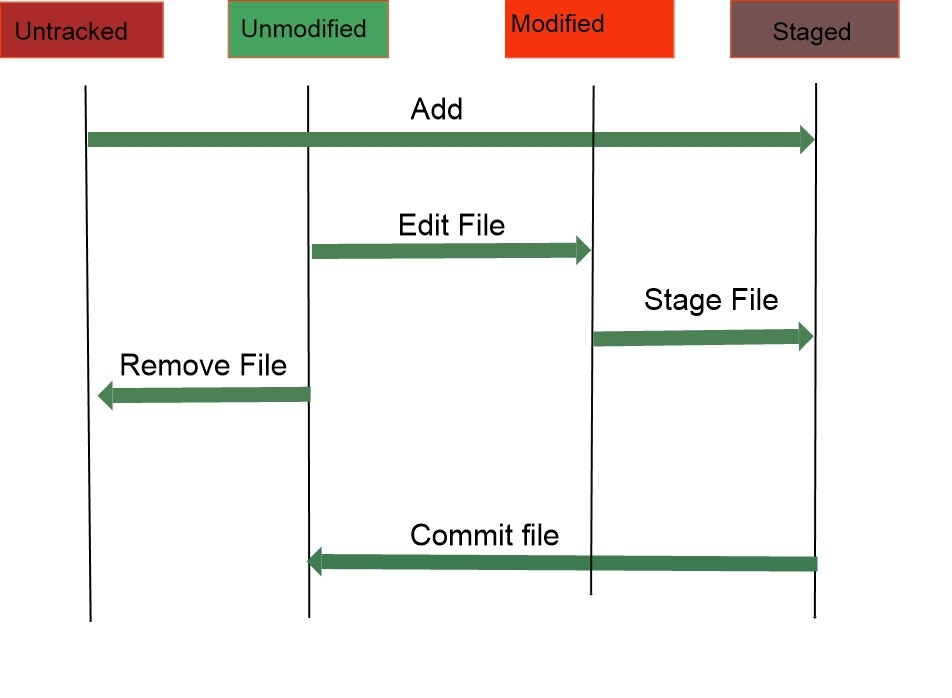
\includegraphics[width=8cm, height = 8cm]{GitHub2.jpg}
\caption{GitHub processing.}
\label{fig:pch}
\end{figure}

\end{enumerate}

When a repository is opened, Git copies files to the working directory\index{Git!working directory} from the database and these may be modified, then staged and then committed.

\subsection{GitHub}

GitHub allows you to store in the cloud and you can work locally using Git.  R packages can be developed using Git and Hadley Wickham's \texttt{devtools} package.  GitHub allows collaborators to work in a controlled way with a shared repo.

Typically, you work locally on your computer in an R project, using Git and then when you are ready to share your package with the world, you \texttt{push} the entire project to GitHub.  There, anybody can access it and install the package directly from GitHub using the command:

\texttt{devtools::install\_github("GitHubUserName/packageName")}.

R packages can be developed using Git and GitHub and Hadley Wickham's \texttt{devtools} package has the capacity to convert a GitHub repo directly into a fully fledged R package.

Git and GitHub useage is integrated into \texttt{Projects} in RStudio.

So let's do it! Firstly, we'll create a RStudio project, but we will get a couple of files ready first. Here's the word-finding script we looked at in Tutorial~\ref{T9}.


\begin{knitrout}
\definecolor{shadecolor}{rgb}{0.969, 0.969, 0.969}\color{fgcolor}\begin{kframe}
\begin{alltt}
   \hlcom{# read in the words from the file, into a vector of mode character}

   \hlstd{txt} \hlkwb{<-} \hlkwd{scan}\hlstd{(}\hlstr{"../Data/tf.txt"}\hlstd{,}\hlstr{""}\hlstd{)}
   \hlstd{tl} \hlkwb{<-} \hlkwd{length}\hlstd{(txt)}
   \hlkwd{cat}\hlstd{(}\hlstr{"The text file was read and there are "}\hlstd{, tl,} \hlstr{" words."}\hlstd{)}
   \hlstd{wl} \hlkwb{<-} \hlkwd{list}\hlstd{()}      \hlcom{# Create a list called wl with no elements}
   \hlkwa{for} \hlstd{(i} \hlkwa{in} \hlnum{1}\hlopt{:}\hlstd{tl) \{}
      \hlstd{wrd} \hlkwb{<-} \hlstd{txt[i]}  \hlcom{# i-th word in input file}
      \hlstd{wl[[wrd]]} \hlkwb{<-} \hlkwd{c}\hlstd{(wl[[wrd]],i)}
   \hlstd{\}}
\hlkwd{print}\hlstd{(wl)}
\end{alltt}
\end{kframe}
\end{knitrout}

Here it is in a functional form:

\begin{knitrout}
\definecolor{shadecolor}{rgb}{0.969, 0.969, 0.969}\color{fgcolor}\begin{kframe}
\begin{alltt}
\hlstd{findWords1} \hlkwb{<-} \hlkwa{function}\hlstd{(}\hlkwc{fn} \hlstd{=} \hlstr{"tf.txt"}\hlstd{) \{}
   \hlcom{# read in the words from the file, into a vector of mode character}
  \hlstd{pfn} \hlkwb{<-} \hlkwd{paste}\hlstd{(}\hlstr{"../Data/"}\hlstd{, fn,} \hlkwc{sep} \hlstd{=} \hlstr{""}\hlstd{)}
  \hlkwd{cat}\hlstd{(}\hlstr{"pfn:  "}\hlstd{,pfn)}
   \hlstd{txt} \hlkwb{<-} \hlkwd{scan}\hlstd{(pfn,}\hlstr{""}\hlstd{)}
   \hlstd{tl} \hlkwb{<-} \hlkwd{length}\hlstd{(txt)}
   \hlkwd{cat}\hlstd{(}\hlstr{"The text file was read and there are "}\hlstd{, tl,} \hlstr{" words."}\hlstd{)}
   \hlstd{wl} \hlkwb{<-} \hlkwd{list}\hlstd{()}      \hlcom{# Create a list called wl with no elements}
   \hlkwa{for} \hlstd{(i} \hlkwa{in} \hlnum{1}\hlopt{:}\hlstd{tl) \{}
      \hlstd{wrd} \hlkwb{<-} \hlstd{txt[i]}  \hlcom{# i-th word in input file}
      \hlstd{wl[[wrd]]} \hlkwb{<-} \hlkwd{c}\hlstd{(wl[[wrd]],i)}
   \hlstd{\}}
   \hlkwd{return}\hlstd{(wl)}
\hlstd{\}}
\end{alltt}
\end{kframe}
\end{knitrout}

Let's run it to see if it still works! (and remind ourselves of what it does.)

\begin{knitrout}
\definecolor{shadecolor}{rgb}{0.969, 0.969, 0.969}\color{fgcolor}\begin{kframe}
\begin{alltt}
\hlkwd{findWords1}\hlstd{(}\hlstr{"tf.txt"}\hlstd{)}
\end{alltt}
\end{kframe}
\end{knitrout}
All is well. Let's now get another of Matloff's word finders:


\begin{knitrout}
\definecolor{shadecolor}{rgb}{0.969, 0.969, 0.969}\color{fgcolor}\begin{kframe}
\begin{alltt}
\hlstd{findWords2} \hlkwb{<-} \hlkwa{function}\hlstd{(}\hlkwc{fn} \hlstd{=} \hlstr{"tf.txt"}\hlstd{) \{}
   \hlcom{# read in the words from the file, into a vector of mode character}
  \hlstd{pfn} \hlkwb{<-} \hlkwd{paste}\hlstd{(}\hlstr{"../Data/"}\hlstd{, fn,} \hlkwc{sep} \hlstd{=} \hlstr{""}\hlstd{)}
  \hlkwd{cat}\hlstd{(}\hlstr{"pfn:  "}\hlstd{,pfn)}
   \hlstd{txt} \hlkwb{<-} \hlkwd{scan}\hlstd{(pfn,}\hlstr{""}\hlstd{)}
   \hlstd{words} \hlkwb{<-} \hlkwd{split}\hlstd{(}\hlnum{1}\hlopt{:}\hlkwd{length}\hlstd{(txt), txt)}
   \hlkwd{return}\hlstd{(words)}
\hlstd{\}}
\end{alltt}
\end{kframe}
\end{knitrout}

Let's test this one, too.

\begin{knitrout}
\definecolor{shadecolor}{rgb}{0.969, 0.969, 0.969}\color{fgcolor}\begin{kframe}
\begin{alltt}
\hlkwd{findWords2}\hlstd{(}\hlstr{"tf.txt"}\hlstd{)}
\end{alltt}
\end{kframe}
\end{knitrout}
Great. Now we have two code files and a data file for our project. The two code files (\texttt{findWords1.R} and \texttt{findWords2.R}  are already in the Code folder in your R\_Course folder, and the data file \texttt{tf.txt} is in the Data folder.

Go to [File->New Project] - select 'New Directory', then select 'R Package', then:

\begin{enumerate}

\item{enter a package name of \underline{your choice - something unique!},}\label{gitName1}
\item{tick the box 'Create a git repository' and}
\item{tick 'Open in a New Session'.}
\item{Browse to choose a suitable sub-directory and}
\item{then add the two R code files.}
\item{click on Create Project.}

\end{enumerate}

Now we see a new RStudio window\index{Git!in RStudio} in which there is an extra Tab for Git in the pane in the top right corner and the File tab in the botttom right corner shows our code files. Before we go any further with this, let's take a quick look at the project folder - if you've forgotten where you put it, it will now be in the header of the Files Tab in the bottom right pane of RStudio's window.  Open Windows Explorer and find the project folder. This is the one you named in Step~\ref{gitName1} of the numbered process above and we will also refer to it as Git's \emph{Working Directory}.

If you can't see a file called \texttt{.gitignore}\index{Git!.gitignore}, in the Working Directory, go to the \emph{View} menu and tick the box, 'Hidden items'. Now, our interest will focus on the following folders and files, which have been automatically generated for our package development:

\begin{itemize}
\item{.gitignore - see below.}
\item{R - a folder containing the source code}
\item{DESCRIPTION - see below}
\item{NAMESPACE - see below}
\end{itemize}

This list should not be seen as exclusive, other important folders you might expect to see in packages include:

\begin{itemize}
\item{data}
\item{tests}
\item{vignette}
\item{demo}
\end{itemize}

.. they are all very important and improve the quality of your package....but we won't deal with these here. (See Hadley Wickham's book \cite{Wickham2015b} or website: \href{http://r-pkgs.had.co.nz/}{http://r-pkgs.had.co.nz}.)


Now, let's get back to those files in the Working Directory. They are standard in a Git working directory and have been set up by RStudio for us.

\subsection{The \texttt{.gitignore} file}
Git will comment on files in the working directory which have not been added.  Since some of our compiling and other processes will generate files which we don't want Git to deal with, we can name them in a file called \texttt{.gitignore}\index{Git!.gitignore}. RStudio sets this up for us with some standard intitial entries.

\subsection{The R folder in the Git Working directory}
Git can be used for any computer language or developing document.  RStudio gave us an R folder on the assumption that our source documents would be R code (or literate R Code). We will add some special comments to these files soon, in order to provide 'nice' documentation when \texttt{help(package= "packageName")} is used.

\subsubsection{Package documentation for the R file}
This is done using the \texttt{roxygen2} package.  Basically, all that is required from us is to have the library loaded and then  modify the function with special comments and a few key words. Here's the listing for a modified version of findWords2() with the documentation added. [Our package function requires the user to specify the path to the data file.]

%\lstloadlanguages{R}
\begin{lstlisting}
#' findwords2: elegant improvement on findwords1
#'
#' @param pfn - a text file
#'
#' @return A list of the words and their sequence number in the file
#' @export

findWords2 <- function(pfn = NULL) {
  # read in the words from the file, into a vector of mode character
  #Matloff p126 (Modified)
  cat("pfn:  ",pfn)
  txt <- scan(pfn,"")
  words <- split(1:length(txt), txt)
  return(words)
}

\end{lstlisting}

The \texttt{roxygen2} comments begin with the \# symbol, followed by a single quotation mark, '. this is followed by a \textbf{single space} and then a special \texttt{roxygen2} label beginning with the ampersand symbol, @.  It will help to take a look at the help page that this generates.  You need to install the package for this.  Here's how:

\begin{knitrout}
\definecolor{shadecolor}{rgb}{0.969, 0.969, 0.969}\color{fgcolor}\begin{kframe}
\begin{alltt}
\hlstd{devtools}\hlopt{::}\hlkwd{install_github}\hlstd{(}\hlstr{"bjw649/testBW1"}\hlstd{)}
\end{alltt}
\end{kframe}
\end{knitrout}
We'll get back to this later, but now we can have a look at what the effect of our strange comments are when the package \texttt{roxygen2} deals with them.

\begin{knitrout}
\definecolor{shadecolor}{rgb}{0.969, 0.969, 0.969}\color{fgcolor}\begin{kframe}
\begin{alltt}
\hlkwd{library}\hlstd{(testBW1)}
\hlkwd{help}\hlstd{(findWords2)}
\end{alltt}
\end{kframe}
\end{knitrout}

If we seek more general help for the package, with \texttt{help(package = "packageName")} the DESCRIPTION folder will be accessed.


\subsection{ The DESCRIPTION folder}\index{Packages!DESCRIPTION folder}
This is \emph{really} important, no matter what you intend doing with your package. If it is just for personal use,  two years' after you last used it, you'll need to look at the description to remember what it was all about!

\begin{lstlisting}

Package: testBW1
Type: Package
Title: Test Package Including Two Word-count Functions
Version: 0.1.0
Authors@R: person("Brian", "Williams", email = "bjw649@gmail.com",
           role = c("aut", "cre"))
Description: This is a test example incorporating two simple functions which do
    word counts.
License: GPL-3
LazyData: TRUE
RoxygenNote: 5.0.1

\end{lstlisting}

This uses a different format again, but it is fairly easy to see what is going on if you look at the help file at the same time:

\begin{knitrout}
\definecolor{shadecolor}{rgb}{0.969, 0.969, 0.969}\color{fgcolor}\begin{kframe}
\begin{alltt}
\hlkwd{help}\hlstd{(}\hlkwc{package}\hlstd{=}\hlstr{"testBW1"}\hlstd{)}
\end{alltt}
\end{kframe}
\end{knitrout}
If on the help page you click on its link to DESCRIPTION file, you will see more of the detail we have included.  For more information about how to format the DESCRIPTION folder take a look at the Hadley Wickham page: \href{http://r-pkgs.had.co.nz/description.html}{http://r-pkgs.had.co.nz/description.html}.


\subsection{The NAMESPACE folder}\index{Packages!NAMESPACE folder}
This is not important for a personal package, but important if you want to submit the package to CRAN or Bioconductor.  It is more complicated than we have time to discuss once again see the book \cite{Wickham2015b} and webpage \href{http://r-pkgs.had.co.nz/namespace.html}{http://r-pkgs.had.co.nz/namespace.html}.

\section{Creating the package}
In the first instance we can create the package directly from our project in RStudio.  With \texttt{devtools} installed its very simple.

\begin{enumerate}
\item{We need to ensure that we have opened the project in RStudio, that we have set the directory to the folder containing the .Rproj file and that \texttt{devtools} is loaded.}
\item{Once that's all in place and our files have all been prepared as described above, we go to the Build tab in the top right pane of RStudio and check to see whether everything has been committed.}
\item{If not we can click on the boxes to stage modified files and then click on commit to store all the changes in the Git database.}
\item{Next we click on the Build tab in the same pane and then on the 'Build and Reload' button beneath it.}
\item{All being well, our package is created (or updated) and the new package is loaded.}
\end{enumerate}

Time to test, but note that if you have the \texttt{testBW1} package loaded along with your own new package, you will need to use the :: notation to ensure that you are testing your own functions and not those in the \texttt{testBW1} package.

\section{Pushing our local repo to GitHub}\index{Git!push local repo to GitHub}

To push this package to our GitHub site we need to have set up a repo on GitHub with the same name as our package/project. It is straightforward.  If you do a fresh login to GitHub, you'll immediately be offered the option of creating a new repo. Do so making sure to use the same name as your RStudio project/package.

Follow the instructions.

Go to the repo and note its URL.

Then, back to RStudio, where You will see that the Git tab offers a 'Push' button. Before you push it, you'll need to tell Git where you want to push it to. SO...

\begin{enumerate}
\item{Check that you are still in the project directory.}
\item{Go to the Tools menu in RStudio and select Shell.}
\item{Enter the following Shell command: \texttt{git remote add origin NotedRepoURL} Where NotedRepoURL is the one you noted above! It will be something like: \texttt{https://GitHub.com/UserName/packageName}.}
\item{Exit from the shell.}
\end{enumerate}

Now you can press the Push button and push it! You'll need your GitHub Username and password to complete the push. You can go back to the GitHub project site and see all your project files and folders have been stored there (securely!).

\section{Creating our package from Github}\index{Packages!create in GitHub}
Remember that your free GitHub site is publicly accessible and so all your friends can install your great new package.  All they have to do is install and load  \texttt{devtools} and then enter the following command:

\begin{knitrout}
\definecolor{shadecolor}{rgb}{0.969, 0.969, 0.969}\color{fgcolor}\begin{kframe}
\begin{alltt}
\hlstd{devtools}\hlopt{::}\hlkwd{install_github}\hlstd{(}\hlstr{"YourGitHubUserName/YourRepoName"}\hlstd{)}
\end{alltt}
\end{kframe}
\end{knitrout}

There's much more to Git and GitHub - they are not that hard to use from RStudio and once you become accustomed to using them , you'll find they are a very useful means of backup and collaboration.

%\printbibliography



% ********  Template for children  ********

% 1. Save as appropriate chapterName (Lecture7, Tutorial10 etc)
% 2. Change title to above
% 3. Change opening chunk name (Temp0) to chapter title
% 4. Remove/replace chunk Temp1

% All chunk names to be preceded by Tn or Ln  (where n is chapter or tutorial number)
% All chunks set eval=evalChild






\chapter{Appendix - miscellaneous extra information}\label{Appendix}


\author{Brian Williams $<$\href{mailto:bjw649@gmail.com}%
{bjw649@gmail.com}$>$}



\section{Relative paths to data files - Lecture 1}\label{DataStructure}

Consider the structure we have in the R\_Course folder.  It corresponds to the structure shown in Figure~\ref{fig:pch}. 

Assume we are working with Lecture1.R in the myRCode folder and we have set the working directory to the myRcode folder.  

Then to find a data file called myData.csv in the Data folder, we can simply find Lecture1.R's parent (the R\_Course folder), and then go to the Data folder (which is also in the R\_Course folder) and find the data file there. 

The relative path (from Lecture1.R to a data file called myData.csv in the Data folder is then "../Data/myData.csv". The 'two-dots' notation takes us to the parent of the current working directory (R\_Course folder)

The absolute paths to the files \emph{could} be included in the code but DON'T DO IT!  It is virtually impossible to use the absolute form if the file is to be accessed by people using different computers, because everybody's absolute  path would be different, depending on where they unpacked their zip file with the Course materials.

If the data file is shared from the web - then a single URL works, but we don't want a classroom of people all accessing a large file at one time!



\begin{figure}[!ht]
\graphicspath{{./Images/}}
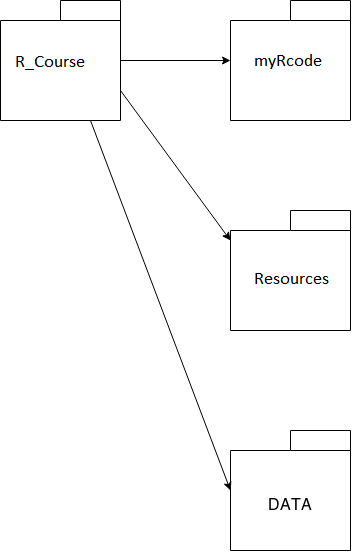
\includegraphics[width=6cm, height = 8cm]{dataFolder2.png}
\caption{Using a common data folder.}
\label{fig:pch}
\end{figure}




\section{Built-in mathematical functions}\index{Functions!built-in, mathematical}
R provides all of the standard mathematical functions that we are familiar with from spreadsheets, calculators etc. 
\begin{knitrout}
\definecolor{shadecolor}{rgb}{0.969, 0.969, 0.969}\color{fgcolor}\begin{kframe}
\begin{alltt}
\hlcom{## Standard mathematical functions in R.}

\hlnum{2} \hlopt{+} \hlnum{4} \hlopt{*} \hlnum{5}      \hlcom{# Note usual order of operations (multiply has precedence)}
\hlkwd{log} \hlstd{(}\hlnum{10}\hlstd{)}       \hlcom{# Natural logarithm with base e=2.7182}
\hlkwd{log10}\hlstd{(}\hlnum{1000}\hlstd{)}      \hlcom{# Common logarithm with base 10}
\hlnum{5}\hlopt{^}\hlnum{3.1}             \hlcom{# 5 raised to the  power 3.1}
\hlnum{5}\hlopt{/}\hlnum{8}             \hlcom{# Division}
\hlnum{8}\hlopt\hlnum{5}            \hlcom{# Remainder of division}
\hlkwd{sqrt} \hlstd{(}\hlnum{20.25}\hlstd{)}      \hlcom{# Square root}
\hlkwd{abs} \hlstd{(}\hlnum{3}\hlopt{-}\hlnum{7}\hlstd{)}     \hlcom{# Absolute value }
\hlstd{pi}                \hlcom{# 3.14}
\hlkwd{exp}\hlstd{(}\hlnum{2}\hlstd{)}         \hlcom{# Exponential function i.e raising 2.7182 to power 2.}
\hlkwd{round}\hlstd{(pi,}\hlnum{4}\hlstd{)}  \hlcom{# Round pi to 4 decimal places}
\hlkwd{floor}\hlstd{(}\hlnum{15.9}\hlstd{)}   \hlcom{# Forces rounding down}
\hlkwd{ceiling}\hlstd{(}\hlnum{15.1}\hlstd{)}  \hlcom{# Forces rounding up }
\hlkwd{cos}\hlstd{(pi}\hlopt{/}\hlnum{3}\hlstd{)}        \hlcom{# Cosine Function}
\hlkwd{sin}\hlstd{(pi}\hlopt{/}\hlnum{2}\hlstd{)}        \hlcom{# Sine Function}
\hlkwd{tan}\hlstd{(pi}\hlopt{/}\hlnum{4}\hlstd{)}       \hlcom{# Tangent Function}
\hlkwd{acos}\hlstd{(}\hlnum{0.5}\hlstd{)}\hlopt{/}\hlstd{pi}        \hlcom{# Inverse Cosine}
\hlkwd{asin}\hlstd{(}\hlnum{0.5}\hlstd{)}\hlopt{/}\hlstd{pi}\hlopt{*}\hlnum{180.}       \hlcom{# Inverse Sine}
\hlkwd{atan}\hlstd{(}\hlnum{0.5}\hlstd{)}\hlopt{/}\hlstd{pi}\hlopt{*}\hlnum{180.}      \hlcom{# Inverse Tangent}
\end{alltt}
\end{kframe}
\end{knitrout}


\section{Probability distributions}
R contains many functions for generating probability distribution data. The function names are organised consistently so that, for example, the density, distribution function, quantile function and random generation for the normal distribution are respectively \texttt{dnorm(), pnorm(), qnorm()} and \texttt{rnorm}.\index{Core functions!dnorm()} \index{Core functions!rnorm()}\index{Core functions!pnorm()}\index{Core functions!qnorm()}for the uniform distribution we would see similarly, \texttt{dunif(), punif(), qunif()} and \texttt{runif}. To see other available distributions in the Core \texttt{stats} package\index{Package!stats}:\index{Package!stats}

\begin{knitrout}
\definecolor{shadecolor}{rgb}{0.969, 0.969, 0.969}\color{fgcolor}\begin{kframe}
\begin{alltt}
\hlkwd{help}\hlstd{(Distributions)}
\end{alltt}
\end{kframe}
\end{knitrout}

Let's have a very quick look at how these functions are used.
Plot the densities:
\begin{knitrout}
\definecolor{shadecolor}{rgb}{0.969, 0.969, 0.969}\color{fgcolor}\begin{kframe}
\begin{alltt}
\hlstd{x} \hlkwb{<-} \hlkwd{seq}\hlstd{(}\hlkwc{from}\hlstd{=} \hlopt{-}\hlnum{3}\hlstd{,} \hlkwc{to} \hlstd{=} \hlnum{3}\hlstd{,} \hlkwc{by} \hlstd{=} \hlnum{0.1}\hlstd{)}
\hlstd{y} \hlkwb{<-} \hlkwd{dnorm}\hlstd{(x)}
\hlstd{x2} \hlkwb{<-} \hlkwd{seq}\hlstd{(}\hlopt{-}\hlnum{3}\hlstd{,}\hlnum{3}\hlstd{,}\hlnum{.2}\hlstd{)}
\hlstd{y2} \hlkwb{<-} \hlkwd{dunif}\hlstd{(x2,}\hlopt{-}\hlnum{3}\hlstd{,}\hlnum{3}\hlstd{)}
\hlkwd{plot}\hlstd{(x,y,} \hlkwc{type} \hlstd{=} \hlstr{"l"}\hlstd{,} \hlkwc{main} \hlstd{=} \hlstr{"Probability density functions"}\hlstd{)}
\hlkwd{points}\hlstd{(x2,y2,} \hlkwc{pch} \hlstd{=} \hlnum{16}\hlstd{)}
\end{alltt}
\end{kframe}
\end{knitrout}

Plot the cumulative distribution functions

\begin{knitrout}
\definecolor{shadecolor}{rgb}{0.969, 0.969, 0.969}\color{fgcolor}\begin{kframe}
\begin{alltt}
\hlstd{y} \hlkwb{<-} \hlkwd{pnorm}\hlstd{(x)}
\hlkwd{plot}\hlstd{(x,y,} \hlkwc{type} \hlstd{=} \hlstr{"l"}\hlstd{,} \hlkwc{main} \hlstd{=} \hlstr{"Cumulative distribution functions"}\hlstd{)}
\hlstd{x2} \hlkwb{<-} \hlkwd{seq}\hlstd{(}\hlopt{-}\hlnum{3}\hlstd{,}\hlnum{3}\hlstd{,}\hlnum{.2}\hlstd{)}
\hlstd{y2} \hlkwb{<-} \hlkwd{punif}\hlstd{(x2,}\hlopt{-}\hlnum{3}\hlstd{,}\hlnum{3}\hlstd{)}
\hlkwd{points}\hlstd{(x2,y2,} \hlkwc{pch} \hlstd{=} \hlnum{16}\hlstd{)}
\end{alltt}
\end{kframe}
\end{knitrout}

Plot the quantile functions

\begin{knitrout}
\definecolor{shadecolor}{rgb}{0.969, 0.969, 0.969}\color{fgcolor}\begin{kframe}
\begin{alltt}
\hlstd{x} \hlkwb{<-} \hlkwd{seq}\hlstd{(}\hlnum{0}\hlstd{,}\hlnum{0.99}\hlstd{,}\hlnum{0.02}\hlstd{)}
\hlstd{y} \hlkwb{<-} \hlkwd{qnorm}\hlstd{(x)}
\hlkwd{plot}\hlstd{(x,y,} \hlkwc{type} \hlstd{=} \hlstr{"l"}\hlstd{,} \hlkwc{main} \hlstd{=} \hlstr{"Quantile functions"}\hlstd{)}
\hlstd{y2} \hlkwb{<-} \hlkwd{qunif}\hlstd{(x)}
\hlkwd{points}\hlstd{(x,y2,} \hlkwc{pch} \hlstd{=} \hlnum{16}\hlstd{)}
\end{alltt}
\end{kframe}
\end{knitrout}

Plot the sampling functions

\begin{knitrout}
\definecolor{shadecolor}{rgb}{0.969, 0.969, 0.969}\color{fgcolor}\begin{kframe}
\begin{alltt}
\hlstd{x} \hlkwb{<-} \hlkwd{rnorm}\hlstd{(}\hlnum{100000}\hlstd{)}
\hlkwd{hist}\hlstd{(x,} \hlkwc{breaks} \hlstd{=} \hlnum{30}\hlstd{,} \hlkwc{main} \hlstd{=} \hlstr{"Histogram of 100000 samples using rnorm()"}\hlstd{)}
\hlstd{x1} \hlkwb{<-} \hlkwd{seq}\hlstd{(}\hlnum{0}\hlstd{,}\hlnum{1}\hlstd{,}\hlnum{1}\hlopt{/}\hlnum{10000}\hlstd{)}
\hlstd{x2} \hlkwb{<-} \hlkwd{runif}\hlstd{(}\hlnum{10001}\hlstd{)}
\hlkwd{plot}\hlstd{(x1,x2,} \hlkwc{main} \hlstd{=} \hlstr{"Scatterplot of 10001 samples from runif"}\hlstd{)}  \hlcom{# Is it really random?}
\end{alltt}
\end{kframe}
\end{knitrout}



\subsection*{Operators}\index{Operators}

In the segment of code above, we saw that two variables could have their values added by using the usual '+' symbol.  As you might expect, R offers a number of symbols to perform such basic functions.  Table~\ref{Operators}, below is the list of operators found in the \href{https://cran.r-project.org/doc/manuals/r-release/R-lang.html#Operators}{Language Reference Manual}.

\begin{table}[!ht]
\begin{tabular}{|r|l|}
\hline
- &	Minus, can be unary or binary\\
+ &	Plus, can be unary or binary\\
! & Unary not\\
\verb+~+ & Tilde, used for model formulae\\
? &	Help\\
: &	Sequence, binary (in model formulae: interaction)\\
\verb+*+ &	Multiplication, binary\\
/ &	Division, binary\\
\verb+^+ &	Exponentiation, binary\\
\verb+%x%+ &	Special binary operators, x is any valid name\\
\verb+%%+ &	Modulus, binary\\
\verb+%/%+ &	Integer divide, binary\\
\verb+%*%+ &	Matrix product, binary\\
\verb+%o%+ &	Outer product, binary\\
\verb+%x%+ &	Kronecker product, binary\\
\verb+%in%+ &	Matching operator for sets, binary \\
< &	Less than, binary\\
> &	Greater than, binary\\
== &	Equal to, binary\\
>= &	Greater than or equal to, binary\\
<= &	Less than or equal to, binary\\
\verb+&+ & And, binary, vectorized\\
\verb+&&+ &	And, binary, not vectorized\\
|	& Or, binary, vectorized\\
|| & 	Or, binary, not vectorized\\
<- & 	Left assignment, binary\\
-> & 	Right assignment, binary\\
\verb+$+ & List subset, binary\\
\hline

\end{tabular}
 \caption{Standard operators in R}
 \label{Operators}
\end{table}

You can access a table like this easily by typing '?Syntax' (without the quotation marks) in the Console pane. The table will appear in the Help Pane (bottom right)

\subsection*{Constants}\index{Constants}

There are 5 types of constants, namely: logical, integer, numeric, complex, string.

In addition there are 4 special constants (which were mentioned above in the 'reserved words'.) The special constants are:
\begin{itemize}
\item{\texttt{NULL} (an object without an assigned value),}\index{Constants!NULL}\index{NULL}
\item{\texttt{NA} (a variable or object with a 'missing' value),}\index{Constants!NA}\index{NA}
\item{\texttt{Inf} (a number whose absolute value is too large for numeric representation - typically resulting from a division by zero),}\index{Inf},\index{Constants!Inf}
\item{\texttt{NaN} ('not a number' - resulting from a division of zero by zero).}\index{Constants!NaN}\index{NaN}
\end{itemize}

Real numeric constants are represented in the usual way:

1.3e7, 1., 1.3, 0.6, .3, 6.3e-4, 16

All of these result in a numeric constant whose type is \texttt{double}.

To assign an numeric constant value of integer type, rather than a numeric, the letter 'L' is added at the end of the integer value. For example, 178L.

String constants\index{String!constants} (sequences of characters, such as a name 'Fred') are delimited either by a pair of single quotes (') or double quotes("). If you need to include one of the pair in the string, it should be preceded by a backslash(\textbackslash). Alternatively, a single quote can be embedded in a string delimited by double quotes and vice-versa. For example we can assign:


\begin{knitrout}
\definecolor{shadecolor}{rgb}{0.969, 0.969, 0.969}\color{fgcolor}\begin{kframe}
\begin{alltt}
\hlstd{stringA} \hlkwb{<-} \hlstr{"the string Henry's"}
\hlstd{stringA}
\hlstd{stringB} \hlkwb{<-} \hlstr{'the string George\textbackslash{}'s'}
\hlstd{stringB}
\end{alltt}
\end{kframe}
\end{knitrout}

There are a number of other special characters which need to be preceded by a backslash ("escaped").  You'll find these in the \href{https://cran.r-project.org/doc/manuals/r-release/R-lang.html#Literal-constants}{Language Reference Manual}.


\begin{itemize}
\item{\texttt{summary()}\index{Core functions!summary()} provides a useful summary of the variables in the data frame (as shown). It computes means, sd, max, min, quartiles of numeric data and for factors (categorical vairables) it provides counts of each category}
 we have already seen the \item{\texttt{str()} function which lists the structure of an object. NOTE that the \texttt{str()} command for space-saving purposes, lists  variables row-by-row, though the data frame actually has them stored as columns. This data frame has many variables which are factors. }
 \item{\texttt{head()}\index{Core functions!head()} shows the first 6 rows (records or cases) of a data frame.}
\end{itemize}






\section{Further reading}
The following are useful references for learning R. The first three are already a little dated, but still contain much useful intrductory information.

Zuur, Ieno et al.\cite{Zuur2009a} uses mostly simple ecological examples with small datasets. It has a strong focus on assembling and manipulating these datasets.

Adler's Nutshell book\cite{Adler2010} contains a wealth of information including parameters used with standard plots and an introduction to the Bioconductor package (which we will discuss later in the course). (There is a new edition which includes material on accessing and analysing web data.)

Dalgaard \cite{Dalgaard2008} contains more basic statistical material, but has a concise well-written introduction to R and a nice compendium of functions.

The books by Kabacoff \cite{Kabacoff2014} (I like this one) and Lander \cite{Lander2014} are more advanced and more recent and cover topics like ggplot2 and creating reports in Word directly from R.

Wickham's book \cite{Wickham2009} on ggplot2 is the standard reference for that material and now there is a second edition. The book by Chang \cite{Chang2012}, provides many more examples and may be an easier starting point.

Crawley's book (\cite{Crawley2012}is a 1000+ page blockbuster.  I have only read the first edition, which had much information, but some of the organization and indexing of subject matter was a little poor.

Wickham's latest books \cite{Wickham2015a, Wickham2015b} are more advanced.  The first cited gives much detail of the underlying properties of R objects and the second provides clear guidelines on how to produce your own R package. 

Munzert et al \cite{Munzert2015} provide a very accessible entry to big data analytics using R packages. Nolan and Temple Lang \cite{Nolan2014} take an in-depth look at R packages for accessing XML and other web technologies. Both these books provide a broad basic background for accessing data from the web, prior to its analysis. Entry-level analysis of 'big data' is now available in many texts, a number of which use R packages for the purpose. A few examples are: Lantz (2013) \cite{Lantz2013}, Forte (2015)\cite{Forte2015} and \cite{Silge2017}. More advanced material with R code can be found in James et al \cite{James2013} and Torgo (2011)\cite{Torgo2011}. And without R code, Bishop's book \cite{Bishop2006} is a very wide-ranging coverage of machine learning.

For reproducible research the book by Xie \cite{Xie2013} describes 'knitr', the software used to create documents containing code and Gandrud's book\cite{Gandrud2013} provides a nice wide-ranging discussion of the various other software and packages which aid production of documents containing reproducible research. A newer book by Xie  \cite{Xie2017} describes the use of the bookdown package which supports creation of technical documents and books.

If you are interested in Event History Analysis, Göran Broström\cite{Brostrom2012} here at Umeå University has written a book on that topic using R.  For related material on survival analysis, Mills' book \cite{Mills2011} comes well recommended (though I have not seen it myself).

Bivand's book\cite{Bivand2008} is the classic for spatial presentation and analysis in R (and there is a new edition), while Dorman\cite{Dorman2014} offers a gentler introduction.
H{\o}jsgaard et al's book\cite{Hojsgaard2012} is a thorough introduction to graphical models (including Bayesian networks) and Nagarajan et al\cite{Nagarajan2013} describe some of the newer methods. Gondro \cite{Gondro2015} introduces R packages used for genomic analysis.

The CRAN website http://www.r-project.org/ has a link to 'Manuals' where there is a free document called 'An introduction to R'. The website also has an extensive (144 in March, 2014) list of books on R. Browsing the web will also uncover many teaching aids and introductory courses.

Finally, and certainly not least are two recent books which have heavily influenced the presentation in these notes. Wickham and Grolemund's 'R for data science'\cite{Wickham2017}, focusses exclusively on rectangular data - dataframes - and since that is by far the form of data of most interest to public health scentists, it provides an excellent basis for using R without the steep learning curve.
Mailund's book \cite{Mailund2017} complements this book with somewhat more advanced material, but with a very similar philosophy.

\subsection{Exercises}
\begin{enumerate}

\item Use \texttt{sample()} to estimate the frequency of a 1 arising from 1 million throws of a dye. 
Use \texttt{runif()} in the range 0-6. What fraction of the data are in the range 0-1

\item Create a sample of 1000000 taken from a N(0,1) distribution.
Compute the fraction of your deviates that are less than 2. Compare with the \texttt{pnorm()} result.
\end{enumerate}


There are some more nice examples at \href{https://nsaunders.wordpress.com/2010/08/20/a-brief-introduction-to-apply-in-r/}{https://nsaunders.wordpress.com/2010/08/20/a-brief-introduction-to-apply-in-r/}

\section{Exercise}

Here is a little function (very slightly modified) from Kabacoff's book\cite{Kabacoff2015}.
Try selecting some numerical variables from the backPain data set and passing them into this function.
Can you think of other statistics you might want to add to the output? It is not hard to add them!

\begin{knitrout}
\definecolor{shadecolor}{rgb}{0.969, 0.969, 0.969}\color{fgcolor}\begin{kframe}
\begin{alltt}
\hlcom{# Slightly modified from Kabacoff's 'R in Action'}
 \hlstd{mystats} \hlkwb{<-} \hlkwa{function}\hlstd{(}\hlkwc{x}\hlstd{,} \hlkwc{na.omit}\hlstd{=}\hlnum{FALSE}\hlstd{)\{}

\hlkwa{if} \hlstd{(na.omit) x} \hlkwb{<-} \hlstd{x[}\hlopt{!}\hlkwd{is.na}\hlstd{(x)]}
\hlstd{m} \hlkwb{<-} \hlkwd{mean}\hlstd{(x)}
\hlstd{n} \hlkwb{<-} \hlkwd{length}\hlstd{(x)}
\hlstd{s} \hlkwb{<-} \hlkwd{sd}\hlstd{(x)}
\hlstd{r} \hlkwb{<-} \hlkwd{range}\hlstd{(x)}
\hlstd{IQR} \hlkwb{<-} \hlkwd{IQR}\hlstd{(x)}
\hlstd{skew} \hlkwb{<-} \hlkwd{sum}\hlstd{((x}\hlopt{-}\hlstd{m)}\hlopt{^}\hlnum{3}\hlopt{/}\hlstd{s}\hlopt{^}\hlnum{3}\hlstd{)}\hlopt{/}\hlstd{n}
\hlstd{kurt} \hlkwb{<-} \hlkwd{sum}\hlstd{((x}\hlopt{-}\hlstd{m)}\hlopt{^}\hlnum{4}\hlopt{/}\hlstd{s}\hlopt{^}\hlnum{4}\hlstd{)}\hlopt{/}\hlstd{n} \hlopt{-} \hlnum{3}
   \hlkwd{return}\hlstd{(}\hlkwd{c}\hlstd{(}\hlkwc{n}\hlstd{=n,} \hlkwc{mean}\hlstd{=m,} \hlkwc{stdev}\hlstd{=s,} \hlkwc{range}\hlstd{= r,} \hlkwc{IQR} \hlstd{= IQR,} \hlkwc{skew}\hlstd{=skew,}
            \hlkwc{kurtosis}\hlstd{= kurt ))}
 \hlstd{\}}
 \hlstd{myvars} \hlkwb{<-} \hlkwd{c}\hlstd{(}\hlstr{"mpg"}\hlstd{,} \hlstr{"hp"}\hlstd{,} \hlstr{"wt"}\hlstd{)}
 \hlkwd{sapply}\hlstd{(mtcars[myvars], mystats)}
\end{alltt}
\end{kframe}
\end{knitrout}



\clearpage
\phantomsection
\addcontentsline{toc}{chapter}{Bibliography}

\printbibliography

\printindex

\end{document}
